% CITA
%I don't care much about music. What I like is sounds.
% Dizzy Gillespie


\RequirePackage{fix-cm} % Technicalities

% -------------------------------------------------------------------------------------------------------------------------
%\documentclass[10pt,b5paper,twoside,showtrims,openright]{memoir}
%\documentclass[10pt,a4paper,twoside,showtrims,openright]{memoir}
\documentclass[11pt,a4paper,twoside,showtrims,openright]{memoir}
% -------------------------------------------------------------------------------------------------------------------------

\usepackage[utf8]{inputenc} % codificacio dels caracters
\usepackage[T1]{fontenc} % Nou esquema de codificacio (recomanat)
%\usepackage{ae,aecompl}
\usepackage[catalan,british,spanish]{babel} % localitzacio de l'estil
\usepackage[UKenglish]{isodate} % per les dates
\usepackage{url} % macro \url per introduir adreces
\usepackage{amssymb,amsmath} % macros per matematiques
\usepackage[pdftex]{graphicx}	% suport per figures
\usepackage{epsfig}
\usepackage{url}
\usepackage{lscape} % per poder posar figures i/o taules en horitzontal
\usepackage{color} % per poder fer servir colors
\usepackage[colorlinks,bookmarks,pdftex,hyperfigures,breaklinks,%backref=page,
  pdfpagemode=UseOutlines,
  pdftitle=Knowledge~Extraction~and~Representation~Learning~for~Music~Recommendation~and~Classification,
  pdfauthor=Sergio~Oramas~Martín,
  pdfsubject=PhD~Thesis,
  pdfkeywords=music~recommendation~knowledge~extraction~representation~learning~multimodal~deep~learning
]{hyperref} % produeix enllacos clicables
\usepackage[round,authoryear]{natbib} % per poder fer citacions Autor-any
%\usepackage{natbibspacing}
%\setlength{\bibspacing}{0.3\baselineskip}
% per les pagines a la bibliografia
% -> UN COMMENT A PARTIR D?AQUI
%\renewcommand*{\backref}[1]{}
%\renewcommand*{\backrefalt}[4]{%
%    \ifcase #1 (Not cited.)%
%    \or        (Cited on page~#2.)%
%    \else      (Cited on pages~#2.)%
%    \fi}

% Packages Sergio
\usepackage{xspace}
\usepackage{subcaption}
\usepackage{tikz-dependency}
\usepackage{csquotes}
\usepackage{bookmark}
\usepackage{textcomp}

\usepackage{fixltx2e} % Technicalities
\usepackage{latexsym}
\usepackage{rotating}
\usepackage{bm}
%\usepackage{bibentry}\nobibliography*
\usepackage{longtable}
%\usepackage{verbatim}
\newsubfloat{figure}
\usepackage{wrapfig}
% better tables
\usepackage[]{threeparttable}
\usepackage{booktabs}
\usepackage{arydshln}
\newcommand{\ra}[1]{\renewcommand{\arraystretch}{#1}}
\usepackage{array}
\newcolumntype{P}[1]{>{\raggedright\arraybackslash}p{#1}}
\newcolumntype{L}[1]{>{\centering\arraybackslash}m{#1}}
\newcolumntype{T}[1]{>{\raggedleft\arraybackslash}p{#1}}
% for footnotes in tables
\usepackage{footnote}
\usepackage{multirow}
\makesavenoteenv{tabular}
\makesavenoteenv{table}

\setlength{\cftpartnumwidth}{0.8cm}

\usepackage{ifthen} % per treure figures de apendix de la llista de figures, etc...

% poerque els footnotes no tornin a comencar a cada chapter
\usepackage{chngcntr}
\counterwithout{footnote}{chapter}

\maxsecnumdepth{subsection} % Per defecte la classe 'memoir' no numera les subseccions. Que les numeri:
\setsecnumdepth{subsection}
\maxtocdepth{subsection} % Tampoc no inclou les subseccions a l'index. Que les inclogui:
\settocdepth{subsection}

% Colors dels enllacos clickables (els que hi ha per defecte son molt kitsch)
\definecolor{NoColor}{rgb}{0,0,0}
\definecolor{LinkColor}{rgb}{0,0,0.25}
\definecolor{ExtLinkColor}{rgb}{0,0.3,0}
\hypersetup{citecolor=NoColor,linkcolor=NoColor,urlcolor=NoColor}

%% Format UPF, dues cares. Recordeu que les dimensions d'A4 i B5 son (210mm,297mm) i (176mm,250mm), respectivament.
\setstocksize{297mm}{210mm} % El suport original es A4
\settrimmedsize{250mm}{176mm}{*} % El suport final, despres de tallar, B5.
\setlength{\trimtop}{23mm} % Alcada de la franja superior a tallar.
\setlength{\trimtop}{24mm} % Alcada de la franja inferior a tallar.
\setlength{\trimedge}{17mm} % Amplada de la franja interior a tallar per cada costat.
%\setulmarginsandblock{*}{29mm}{1.1} % Marges verticals (3cm a dalt, 0.9*3cm a baix)
%\setlrmarginsandblock{30mm}{*}{0.75} % Marges laterals (3cm a la dreta, 0.75*3cm l'esquerra)
\setulmarginsandblock{23mm}{18mm}{*} % used to be {25mm}{16mm}
\setlrmarginsandblock{25mm}{*}{0.8}
\checkandfixthelayout
\trimLmarks % Marques de tall en forma de 'L'

% arreglar que floats al final de capitol no es centrin verticalment
%\makeatletter% Set distance from top of page to first float
%\setlength{\@fptop}{5pt}
%\makeatother

% perque no es posi espai blanc raro entre coses
%\raggedbottom
\flushbottom

% espai despres de floats
\setlength{\textfloatsep}{0.5cm}


% Estil de quan poso tags al text tags
\newcommand{\atag}[1]{\small{\texttt{#1}}\normalsize}

% Estil dels capitols (consulteu estils disponibles a http://www.imf.au.dk/system/latex/artikler/MemoirChapStyles/MemoirChapStyles.pdf)
%\chapterstyle{veelo}
%\chapterstyle{ell}
%\chapterstyle{bianchi}
%\makechapterstyle{myveelo}{
%  \setlength{\afterchapskip}{40pt}
%  \renewcommand*{\chapterheadstart}{\vspace*{40pt}}
%  \renewcommand*{\afterchapternum}{\par\nobreak\vskip 25pt}
%  \renewcommand*{\chapnamefont}{\normalfont\LARGE\flushright}
%  \renewcommand*{\chapnumfont}{\normalfont\HUGE}
%  \renewcommand*{\chaptitlefont}{\normalfont\HUGE\bfseries\flushright}
%  \renewcommand*{\printchaptername}{\chapnamefont CHAPTER} %\renewcommand*{\printchaptername}{\chapnamefont\MakeUppercase{\@chapapp}}
%  \renewcommand*{\chapternamenum}{}
%  \setlength{\beforechapskip}{18mm}
%  \setlength{\midchapskip}{\paperwidth}
%  \addtolength{\midchapskip}{-\textwidth}
%  \addtolength{\midchapskip}{-\spinemargin}
%  \renewcommand*{\printchapternum}{
%    \makebox[0pt][l]{
%      \hspace{.8em}
%      \resizebox{!}{1cm}{\chapnumfont \thechapter} %\resizebox{!}{\numberheight}{\chapnumfont \thechapter}
%      \hspace{.8em}
%      \rule{\midchapskip}{\beforechapskip}
%    }
%  }
%  \makeoddfoot{plain}{}{}{\thepage}
%}

\makechapterstyle{myveelo}{
  \renewcommand*{\chapterheadstart}{\vspace*{0.7cm}}
  \renewcommand*{\chapnamefont}{\normalfont\Large}
  \renewcommand*{\chapnumfont}{\normalfont\HUGE}
  \renewcommand*{\chaptitlefont}{\vspace*{-2.1cm}\normalfont\HUGE\bfseries\flushright}
  \renewcommand*{\printchaptername}{\flushright \chapnamefont CHAPTER\ \ \ \ \ \ \ \ }
  \setlength{\beforechapskip}{12mm}
  \setlength{\midchapskip}{\paperwidth}
  \addtolength{\midchapskip}{-\textwidth}
  \addtolength{\midchapskip}{-\spinemargin}
  \setlength{\afterchapskip}{2cm}
  \renewcommand*{\printchapternum}{
    \makebox[0pt][l]{
      \hspace{-1cm}
      \resizebox{!}{1cm}{\chapnumfont \thechapter}
      \hspace{0.4cm}
      \rule{\midchapskip}{\beforechapskip}
    }
  }
  \makeoddfoot{plain}{}{}{\thepage}
}

%\usepackage{calc}\usepackage{tikz}
%\makechapterstyle{mycombined}{
%  \setlength{\beforechapskip}{1cm}
%  \setlength{\midchapskip}{-80pt}
%  \setlength{\afterchapskip}{2cm}
%  \renewcommand*{\printchaptername}{}
%  \renewcommand*{\chapnumfont}{\normalfont\bfseries\fontsize{60}{0}\selectfont}
%  \renewcommand*{\printchapternum}{
%    %\flushright\chapnumfont\thechapter
%    \flushright 
%    %\normalfont\large\bfseries Chapter
%    \begin{tikzpicture}
%      \draw[fill,color=black] (0,0) rectangle (2cm,2cm);
%      \draw[color=white] (1cm,1cm) node { \chapnumfont\thechapter };
%    \end{tikzpicture}
%    \marginpar{}
%  }
%  \renewcommand*{\chaptitlefont}{\normalfont\HUGE\bfseries}
%  \renewcommand*{\printchaptertitle}[1]{%
%    \raggedright\chaptitlefont\parbox[t]{\textwidth-3cm}{\raggedright##1}}
%}

%\chapterstyle{mycombined}
\chapterstyle{myveelo}

% Labels when enumerating
%\renewcommand{\labelenumi}{\alph{enumi})}
%\renewcommand{\labelenumii}{\alph{enumii})}

% ---- Some configs...

\usepackage[font=small,labelfont=bf]{caption}

%\renewcommand{\rmdefault}{put}
%\renewcommand{\sfdefault}{phv}
\newcommand{\superscript}[1]{\ensuremath{^{\textrm{#1}}}}
\newcommand{\subscript}[1]{\ensuremath{_{\textrm{#1}}}}
\newcommand{\quotat}[2]{
  \begin{flushright}
    \textit{``#1'',\\
    \vspace*{0.3cm}
    #2.\\
    \vspace*{0.3cm}
    }
  \end{flushright}
}
%\newcommand{\comentari}[1]{\textcolor{red}{\textbf{[#1]}}}
\DeclareMathOperator*{\argmax}{arg\,max}
\DeclareMathOperator*{\argmin}{arg\,min}
\DeclareMathOperator*{\argsort}{\text{argsort}}

% Space between paragraphs and lines
\setlength{\parskip}{1.4mm} % space between paragraphs
%\setlength{\parskip}{1mm plus1mm minus1mm}

%\linespread{1.35}
\linespread{1}

% Bullet points index esquema
%\newcommand{\point}{\vspace{0.25cm}$\bullet$\hspace{0.25cm}}
\newcounter{points}
\definecolor{orange}{rgb}{1,0.5,0}
\newcommand*\point{%
  \stepcounter{points}%
  \vspace{0.25cm}
  \textcolor{orange}{$\bullet^{\thepoints}$}
  }

% pel tema git

%\usepackage{totcount}
%\regtotcounter{points}
%\usepackage{eso-pic}% http://ctan.org/pkg/eso-pic
%\input{gitHeadInfo}
%\newcommand{\gitInfo}{Commit info: \gitShortHash\gitDirty, \gitDate}
%\AddToShipoutPictureBG{% Add picture to background of every page
%  \AtPageLowerLeft{%
%    \raisebox{1.2\baselineskip}{\makebox[\paperwidth]{\begin{minipage}{21cm}\centering
%      %\textcolor{orange}{\gitInfo \hspace{0.15cm}(\total{points} points)}
%      \textcolor{orange}{\gitInfo}
%    \end{minipage}}}%
%  }
%}

% per definir mides de figures
\newcommand{\figSizeMax}{1.0\columnwidth}
\newcommand{\figSizeLarge}{0.8\columnwidth}
\newcommand{\figSizeMidLarge}{0.7\columnwidth}
\newcommand{\figSizeMid}{0.6\columnwidth}
\newcommand{\figSizeMidSmall}{0.5\columnwidth}

% Variables matematiques i altres
\usepackage{color}
\definecolor{darkgreen}{rgb}{0,0.5,0}
\newcommand{\TODO}[1]{{\color{red}{[{TODO:} #1}]}}
\newcommand{\COMMENT}[1]{{\color{darkgreen}{[#1}]}}
\newcommand{\XXX}[3]{{\color{blue}{{[#1$\rightarrow$#2:} #3{]}}}}
% Uncomment next line to hide all comments
%\renewcommand{\XXX}[3]{}
%\renewcommand{\TODO}[1]{}
%\renewcommand{\COMMENT}[1]{}

% Necessari per una de les equacions (perquè es vegi bé)
\def\mathLarge#1{\mbox{\LARGE $#1$}}


%quote al final
\renewenvironment{quotation}
  {\begin{trivlist} \setlength\leftskip{2cm} \setlength\rightskip{0pt}
   \item\relax}
  {\end{trivlist}}


%OJO PONER DE NUEVO
%%i, j, k, m, n, u, v, r -> indexs

%----- !!! coses rares:
%- u -> user i també index en algun cas
%- r -> resource i també posició d'un candidate tag a la llista de candidates
%- \alpha -> user for statistical significance threshold and percentage parameter in percentage strategy
%- N, n used for days vector in impact analysis
%- R -> used as reference window indicator and as recall
%- \varrho used for spearman rank coefficient and number of repeated candidate tags
%-----

% General tag recommendation
\newcommand{\users}{\mathbf{U}}
\newcommand{\user}{u}
\newcommand{\tags}{\mathbf{T}}
\renewcommand{\tag}{t} % Watch out, overwritting \tag command
\newcommand{\tagb}{t}
\newcommand{\resources}{\mathbf{R}}
\newcommand{\resource}{r}
\newcommand{\nRecommendedTagsInEvaluation}{\kappa} % algorithm parameter
\newcommand{\inputTags}{\tags_{\text{I}}}
\newcommand{\inputTag}{\tags_{\text{I}_i}}
\newcommand{\candidateTags}{\tags_{\text{C}}}
\newcommand{\candidateTagsPerInputTag}{\candidateTags^i}%{\tags^i_{\text{C}}}
\newcommand{\candidateTagsPerInputTagOne}{\candidateTags^1}
\newcommand{\candidateTagsPerInputTagTwo}{\candidateTags^2}
\newcommand{\recommendedTags}{\tags_{\text{R}}}
\newcommand{\aggregatedCandidateTags}{\tags_{\text{A}}}
\newcommand{\folksonomy}{\mathcal{F}}
\newcommand{\nCandidateTagsPerInputTag}{\theta} % algorithm parameter
\newcommand{\similarityMatrix}{\mathcal{S}}
\newcommand{\similarityMatrixElement}{s}
\newcommand{\graph}{\mathcal{G}}
\newcommand{\vertices}{\mathbf{V}}
\newcommand{\edges}{\mathbf{E}} % tag application
\newcommand{\tagApplication}{\edges} % tag application
\newcommand{\associationMatrix}{\mathcal{D}}
\newcommand{\associationMatrixElement}{d}
\newcommand{\associationMatrixMultiplication}{\mathcal{DD}}
\newcommand{\associationMatrixRow}{\mathbf{D}}
\newcommand{\bipartiteGraphTagsResources}{\mathcal{TR}} %\tags\resources}}
\newcommand{\bipartiteGraphTagsUsers}{\mathcal{TU}} %\tags\resources}}
\newcommand{\bipartiteGraphUsersResources}{\mathcal{UR}} %\tags\resources}}
\newcommand{\scoreCandidateTag}{\phi}
\newcommand{\candidateTag}{\tags^i_{\text{C}_j}}
\newcommand{\positionOfCandidateTagInList}{n}
\newcommand{\scoreThreshold}{\varepsilon} % algorithm parameter
\newcommand{\percentageOfPercentageStrategy}{\alpha} % algorithm parameter
\newcommand{\probabilityDensityFunction}{\text{PDF}}
\newcommand{\percentageOfKernelPercentageStrategy}{\beta}  % algorithm parameter
\newcommand{\andersonDarlingTest}{\text{AD}}
\newcommand{\histogram}{\text{HIST}}
\newcommand{\deletedTags}{\tags_{\text{D}}}
\newcommand{\precision}{P}
\newcommand{\recall}{R}
\newcommand{\fmeasure}{F}
\newcommand{\contentFeature}{f}
\newcommand{\nRepeatedCandidateTags}{\varrho} % algorithm parameter
\newcommand{\differenceNRecTagsAndNDelTags}{\Delta_{\tags}}
\newcommand{\pvalue}{p}
\newcommand{\gaussianMean}{\mu}
\newcommand{\gaussianStDev}{\sigma}
\newcommand{\tagFrequencyThreshold}{\omega}  % algorithm parameter

% Class-basesd recommendation
\newcommand{\audioClip}{\resource}%{a}
\newcommand{\nAudioClasses}{H}
\newcommand{\audioClasses}{\mathbf{C}}
\newcommand{\audioClass}{\audioClasses_{h}}%{c}
\newcommand{\similarityMatrixOfClass}{\mathcal{S}_{\audioClass}}%{\mathcal{S}_\text{C}}
\newcommand{\similarityMatrixOfClassH}{\similarityMatrixOfClass}%{\mathcal{S}_{\text{C}_h}}
\newcommand{\associationMatrixOfClass}{\mathcal{D}_{\audioClass}}%{\mathcal{D}_\text{C}}
\newcommand{\associationMatrixOfClassH}{\associationMatrixOfClass}%{\mathcal{D}_{\text{C}_h}}
\newcommand{\tagsUsedToAnnotateAudioClip}{\tags_{\text{P}}}
\newcommand{\numberOfTagRecommendationsInSession}{M}
\newcommand{\recommendationsInSessionIndex}{m}
\newcommand{\nthRecommendedTagsInSession}{\tags_{\text{R}}^{\resource, \recommendationsInSessionIndex}}
\newcommand{\nAcceptedTags}{\Omega}  % Metric
\newcommand{\statisticalSignificanceThreshold}{\alpha}
\newcommand{\spearmanCorrelationCoefficient}{\varrho}
\newcommand{\nAudioClipsEvaluatedInComplementaryEvaluation}{N}
\newcommand{\audioClipEvaluatedInComplementaryEvaluation}{n}

% Impact of tag recommendation
\newcommand{\timePeriod}{t}
\newcommand{\daysVector}{\mathbf{D}}
\newcommand{\window}{W}
\newcommand{\referenceWindowIndicator}{R}
\newcommand{\referenceWindowsVector}{\mathbf{\window}}%^\referenceWindowIndicator}
\newcommand{\windowOfInterest}{\window_I}
\newcommand{\metricVocabularyConvergence}{\Theta}  % Metric
\newcommand{\setOfNewTagsInDay}{\tags_{\text{NEW}}^{n}}
\newcommand{\setOfTagApplicationsInADay}{\tagApplication^{n}}
\newcommand{\setOfTagApplicationsInADayWithMisspellings}{\tagApplication_{\text{MISS}}^{n}}
\newcommand{\metricAverageVocabularySize}{\Upsilon}  % Metric
\newcommand{\setOfUsersPerformingTagApplicationInDay}{\users^{n}}
\newcommand{\setOfTapplicationsDistinctTagsPerUserAndDay}{\tagApplication^{\user,n}}
\newcommand{\usersNetwork}{\mathcal{U}} % \users
\newcommand{\edgeWeight}{w}
\newcommand{\setOfDistincTagsPerUserAndPeriod}{\tags^{i,k}}
\newcommand{\setOfDistincTagsPerUserAndPeriodJ}{\tags^{j,k}}
\newcommand{\metricUserVocabularySharing}{\Psi_{\text{u}}}  % Metric
\newcommand{\nNodes}{L}
\newcommand{\soundsNetwork}{\mathcal{R}} % \users
\newcommand{\tagsAssignedToSoundI}{\tags^{i}}
\newcommand{\tagsAssignedToSoundJ}{\tags^{j}}
\newcommand{\metricSoundVocabularySharing}{\Psi_{\text{r}}}  % Metric
\newcommand{\metricAverageTaglineLength}{\Gamma}  % Metric
\newcommand{\tagApplicationsPerResourceR}{\tagApplication^\resource}
\newcommand{\soundsUploadedInDay}{\resources^n}
\newcommand{\tagFrequency}{\upsilon}
\newcommand{\tagApplicatonsPerTagT}{\tagApplication^{\tagb,k}}
\newcommand{\qualityJudgement}{q}
\newcommand{\metricQualitativeAnnotationQuality}{Q}  % Metric
\newcommand{\unionOfQualityJudgements}{\mathbf{Q}}  %{\varkappa} 
\newcommand{\metricAverageTagApplicationTime}{\Phi_{\text{e}}}   % Metric
\newcommand{\annotationSession}{a}
\newcommand{\annotationSessions}{\mathbf{A}}
\newcommand{\durationOfAnnotationSessionAux}{\lambda}
\newcommand{\durationOfAnnotationSession}{\durationOfAnnotationSessionAux_\annotationSession}
\newcommand{\tagApplicationsOfAnnotationSession}{\tagApplication^\annotationSession}
\newcommand{\metricPercentageOfCorrectlyPredictedTags}{\nAcceptedTags}%{\breve\Omega}   % Metric
\newcommand{\tagsOfSoundR}{\tags^\resource}
\newcommand{\setOfTagsSuggestedToSoundR}{\tagsOfSoundR_{\text{S}}}
\newcommand{\subjectiveEvaluationSetX}{\mathbf{X}}
\newcommand{\subjectiveEvaluationSetY}{\mathbf{Y}}
\newcommand{\metricMispellings}{M} % Metric
\newcommand{\nodeStrength}{\vartheta}



% Ontology tag recommendation
\newcommand{\ontology}{\mathcal{O}}
\newcommand{\tagCategoriesAux}{Z}
\newcommand{\tagCategories}{\mathbf{\tagCategoriesAux}}
\newcommand{\tagCategory}{z}%{\tagCategories_{l}}%{z}
\newcommand{\recommendedTagCategories}{\tagCategories_\text{R}}
\newcommand{\populationForTagCategory}{\tags_{\text{\tagCategoriesAux}}}
\newcommand{\populationForTagCategoryL}{\tags^{\tagCategory}_{\text{\tagCategoriesAux}}}
\newcommand{\postPopulationForTagCategoryL}{\tags^{\tagCategory}_{\text{\tagCategoriesAux}^\prime}}
\newcommand{\metricAverageTimePerAudioClip}{\Phi_{\text{r}}}
\newcommand{\metricPercentageOfAttributeTags}{\Pi}
\newcommand{\metricAnnotationComprehensiveness}{\Lambda}
\newcommand{\metricCoherenceInAnnotations}{I} 
\newcommand{\setOfAttributeTags}{\tags_{\text{T}}} 
\newcommand{\groundTruthForResourceR}{\mathbf{G}^\resource} 
\newcommand{\recommendedTagsPerTagCategory}{\recommendedTags^\tagCategory}%{\recommendedTags | \tagCategory}








% ************ Lines for draft mode ************
% \usepackage[top=3cm,bottom=3cm,left=3cm,right=3cm,bindingoffset=0.8cm,includeheadfoot,paper=a4paper]{geometry}
% \linespread{1.6}
% **********************************************


\hyphenation{Universitat Pompeu Fabra}


%------------------------------------------------------------------------------------------------
% -----------------------------------------------------------------------------------------------
%------------------------------------------------------------------------------------------------
%------------------------------------------------------------------------------------------------

\begin{document}
\parindent0ex
\selectlanguage{british}
\setlength\emergencystretch{\hsize}

% ------------------------------------------------------------

\newpage
\thispagestyle{empty}
\begin{titlingpage}
\begin{flushright}

  \begin{figure}[t]
    \begin{flushright}
      %
\includegraphics[width=4.5cm]{ch00/pics/logo_upf.jpg}
      
\includegraphics[width=4.5cm]{ch00_pics/upf-logo-bo}
    \end{flushright}
  \end{figure}

  \vspace*{2.2cm} 

  %\begin{center}
  %\line(1,0){372}

  %{\huge \textbf{Identification of Versions of the \\ Same Musical Composition by \\ \vspace*{0.23cm} Processing Audio Descriptions}}
  %{\Large \textbf{IDENTIFICATION OF VERSIONS \\ \vspace*{0.1cm} OF THE SAME MUSICAL COMPOSITION \\ \vspace*{0.25cm} BY PROCESSING AUDIO DESCRIPTIONS}}
  %{\huge \textbf{Tag Recommendation for Online \\Sound Sharing Based on Folksonomy Analysis}}
  %{\huge \textbf{Tag Recommendation using \\ Folksonomy Information for \\ \vspace*{0.25cm}Online Sound Sharing Platforms}}
  %{\LARGE \textbf{\textsc{Identification of Versions of \\ \vspace*{0.05cm} the Same Musical Composition \\ \vspace*{0.25cm} by Processing Audio Descriptions}}}
  {\huge \textbf{Knowledge Extraction and \\ \vspace*{0.15cm} Representation Learning for \\ \vspace*{0.10cm} Music Recommendation \\ \vspace*{0.45cm} and Classification}}

  \vspace*{2cm}

  %{\textbf{Joan Serr\`a Juli\`a}}
  {\Large \textbf{Sergio Oramas Martín}}
  %{\Large Joan Serr\`a Juli\`a}
  %{Joan Serr\`a Juli\`a}

  %\line(1,0){372}
  %\end{center}
   
  \vspace*{\fill} 
  TESI DOCTORAL UPF / 2017

\end{flushright}
  
  \vspace*{1.5cm}

  Director de la tesi:

  \vspace*{-0.25cm}

  \line(1,0){372}
  
  \vspace*{0.25cm}

  Dr.~Xavier Serra Casals

  Dept.~of Information and Communication Technologies

  Universitat Pompeu Fabra, Barcelona, Spain
  
%\end{flushright}
\end{titlingpage}
\selectlanguage{british}

% ------------------------------------------------------------

\frontmatter
%\newpage
\cleartorecto
\thispagestyle{empty}

{\footnotesize Copyright~\textcopyright~Sergio Oramas Martin, 2017.}
\\{\footnotesize Licensed under \href{http://creativecommons.org/licenses/by-nc-sa/3.0/}{Creative Commons Attribution-NonCommercial-ShareAlike 3.0 Unported}.}

\href{http://creativecommons.org/licenses/by-nc-sa/3.0/}{
\includegraphics[width=3cm]{ch00_pics/creative-commons2.png}}


\vspace*{5cm}

%\begingroup
%\leftskip2em
%\rightskip\leftskip

Dissertation submitted to the Deptartment of Information and Communication Technologies of Universitat Pompeu Fabra in partial fulfillment of the requirements for the degree of

\vspace*{0.5cm}

\centerline{DOCTOR PER LA UNIVERSITAT POMPEU FABRA}

\vspace*{0.6cm}


%\par
%\endgroup

\vspace*{\fill}

\line(1,0){372}\\
\footnotesize
Music Technology Group (\url{http://mtg.upf.edu}), Dept.~of Information and Communication Technologies (\url{http://www.upf.edu/dtic}), Universitat Pompeu Fabra (\url{http://www.upf.edu}), Barcelona, Spain.
\normalsize

% ------------------------------------------------------------

\cleartorecto
\thispagestyle{empty}


\noindent By My Self and licensed under

\noindent
\href{http://creativecommons.org/licenses/by-nc-nd/3.0/}{Creative Commons Attribution-NonCommercial-NoDerivs 3.0 Unported}

\noindent
\href{http://creativecommons.org/licenses/by-nc-nd/3.0/}{
\includegraphics{ch00/pics/creative-commons.png}}

\vfill

\noindent You are free to Share -- to copy, distribute and transmit the work
Under the following conditions:

\begin{itemize}
\item \textbf{Attribution} -- You must attribute the work in the manner
  specified by the author or licensor (but not in any way that
  suggests that they endorse you or your use of the work).
\item 
  \textbf{Noncommercial} -- You may not use this work for commercial purposes.
\item 
  \textbf{No Derivative Works} -- You may not alter, transform, or build upon
  this work.
\end{itemize}

\noindent With the understanding that:

\begin{description}
\item[Waiver] -- Any of the above conditions can be waived if you
  get permission from the copyright holder.  
\item[Public Domain] -- Where
  the work or any of its elements is in the public domain under
  applicable law, that status is in no way affected by the license.
\item[Other Rights] -- In no way are any of the following rights affected
  by the license: 
  \begin{itemize}
  \item Your fair dealing or fair use rights, or other applicable
    copyright exceptions and limitations;
  \item The author's moral rights;
  \item Rights other persons may have either in the work itself or in how
    the work is used, such as publicity or privacy rights.
  \end{itemize}
\item[Notice] -- For any reuse or distribution, you must make clear to
  others the license terms of this work. The best way to do this is
  with a link to this web page.
\end{description}



%%% Local Variables: 
%%% mode: latex
%%% TeX-master: "thesis"
%%% End: 



% ------------------------------------------------------------

\cleartorecto

\newcommand\advisor[2]{
	\vspace{1.3cm}
	\begin{center}
		\rule{6cm}{0.8pt}\\
		\textbf{#1}\\
		(Thesis Supervisor)\\
		#2
	\end{center}
}
\newcommand\member[2]{
	\vspace{1.3cm}
	\begin{center}
		\rule{6cm}{0.8pt}\\
		\textbf{#1}\\
		(Thesis Committee Member) \\
		#2
	\end{center}
} 

%\begin{itemize}
%\item[] Chairman
%\item[] Member
%\item[] Member
%\item[] Member
%\item[] Secretary
%\end{itemize}
\vspace{1cm}
\noindent The doctoral defense was held on ......................... at the Universitat Pompeu Fabra and scored as ...........................................................\par
\vspace{2cm}
\advisor{\supervisor}{Universitat Pompeu Fabra (UPF), Barcelona, Spain}
\vspace*{0.3cm}
%\begin{center}
%\large{\textbf{Thesis committee}}
%\end{center}

\member{Dr. Markus Schedl}{Johannes Kepler University, Linz, Austria}
\member{Dr. Emilia G{\'o}mez}{Universitat Pompeu Fabra (UPF), Barcelona, Spain}
\member{Dr. Brian Whitman}{Spotify, Boston, USA}

% ------------------------------------------------------------

\cleartorecto
\thispagestyle{empty}
\selectlanguage{catalan}
\vspace*{3cm}
\begin{flushright}
\textit{a Olivia y Chiara, la luz en el camino...}
\end{flushright}
\selectlanguage{british}

% ------------------------------------------------------------

\cleartorecto
\chapter*{Acknowledgements}
First of all, I would like to thank my supervisor, Dr. Xavier Serra, for giving me the opportunity to work in this fantastic environment, the Music Technology Group, and for his wise advises. Also, I want to give special thanks to Paco Gomez for teaching me how to be a researcher. This thesis does not have a specific co-supervisor, but along this journey I have met three great researchers and better persons who have helped me through my PhD and without whom this work would have not been possible, Mohamed Sordo, Vito Claudio Ostuni, and Oriol Nieto. 
Special thanks also to Frederic Font with whom I have shared through all these years office, research, music, and friendship.
A very important element of this thesis has been my collaboration with the TALN group. Everything started sharing pizza and water and now we have a lot papers together and thousands of ideas. It was great collaborating and partying with Luis Espinosa-Anke and Francesco Barbieri. Also special thanks to Horacio Saggion for his wise advises, and Tommaso Di Noia, Aonghus Lawlor and Michael O'Mahony for hosting me during my research stays at Politecnico de Bari and University College of Dublin. 
A special mention to Ichiro Fujinaga and Susan Weiss, who strongly believed in my research line. Also to my COFLA mates Emilia Gómez, Joaquin Mora and José Miguel Díaz-Báñez, thanks for considering me a researcher from the first day.
To my Pandora managers Andreas Ehmann, Oscar Celma, and Fabien Gouyon, who trusted me and gave me the opportunity to apply my research in the real world.

I also want to thank other amazing MTG people who shared with me knowledge and laughs throughout these years. In no specific order, thanks to the SIC-refugio team
Sebastian Mealla, Álvaro Sarasúa, Panos Papiotis. To Rafael Caro, my musicologist mate. To Oriol Romaní and Juanjo Bosh for so much fun. To Alastair Porter and Dmitry Bogdanov for their experience and friendship. To Andrés Ferraro who shared my vision and helped me in the development of my ideas. To Gopala Koduri and our conversations about semantics. To Jordi Pons for initiating me in the deep learning cult. To my new roommates Eduardo Fonseca, Xavier Favory, and former roommates Gerard, Dara, Hector, Giuseppe, and Albin. To even more great people I met in the MTG, Cárthach, Ángel, Dani, Marius, Alfonso, Sergio, Zacharias, Olga, Perfe, Rong and Georgi. To former members, Sankalp, Sertan, Sercan, Ajay, Justin, Nadine and Martí. To Joan and Miguel from the TALN. To Humberto from UCD. To my Pandora mates Massimo, Theo, Chun and Andreu. Sorry if I forgot to mention anyone.
Also thanks to Aurelio, Lydia, Sonia, Cristina, Magda, Jana and Alba for helping me with the administrative work.
Special thanks to Obra Social "La Caixa" and their fellowship program, to believe in me and support this research.

Last but not least, this work would have been never been possible without the support of my wife Chiara, who followed me to Barcelona and helps me to persue my dreams. Also to my lovely Olivia, I started my PhD and my paternity at the same time, and I am pretty sure these have been the happiest years of my life. Finally, many thanks to my parents, brothers and sisters, who helped me so much along my whole life, I am here thanks to them.

\vspace*{\fill}

\line(1,0){372}\\
\footnotesize
This thesis has been carried out at the Music Technology Group of Universitat Pompeu Fabra (UPF) in Barcelona, Spain, from October~2013 to September~2017, at the Politecnico di Bari, Italy, from September~2014 to October~2014, at the Insight Centre for Data Analytics of University College of Dublin (UCD), Ireland, from May~2015 to July~2015, and at Pandora Media Inc., USA, from June~2016 to September2016. This work has been supported by Obra Social "La Caixa" under their graduate fellowship program, and by the Spanish Ministry of Economy and Competitiveness under the Maria de Maeztu Units of Excellence Programme (MDM-2015-0502). The research stay at UCD has been also funded by the Keystone COST Action IC1302 under grant number SFI/12/RC/2289. Parts of the work presented in this thesis were partly supported by the European Research Council under the European Union's Seventh Framework Program, as part of the CompMusic project (ERC grant agreement 267583), and by the COFLA2 research project (Proyectos de Excelencia de la Junta de Andalucia, FEDER P12-TIC-1362).
\normalsize

% ------------------------------------------------------------

\cleartorecto
%\thispagestyle{empty}
\chapter{Abstract}
%\addcontentsline{toc}{chapter}{Abstract}
Music content creation, publication and dissemination has changed dramatically in the last few decades. Huge amounts of information about music are being published daily in online repositories such as web pages, forums, wikis, and social media. However, most of this content is still unusable by machines due to the fact that it is mostly created by humans and for humans. Furthermore, online music services currently offer ever-growing collections with tens of millions of music tracks. This vast availability has posed two serious challenges. First, how can a musical item be properly annotated and classified within a large collection? Second, how can a user explore or discover preferred music from all of the available content? In this thesis, we address these two questions by focusing on the semantic enrichment of descriptions associated to musical items (e.g., artists biographies, album reviews, metadata), and the exploitation of the heterogeneous data in large music collections (e.g., text, audio, images). To this end, we first focus on the problem of linking music-related texts with online knowledge repositories via entity linking, and on the automated construction of music knowledge bases via relation extraction. Then, we investigate how extracted knowledge may impact recommender systems, classification approaches, and musicological studies. We show how modeling semantic information helps to outperform text-based approaches in artist similarity and music genre classification, and achieves significant improvements with respect to state of the art collaborative algorithms in music recommendation, while promoting long tail recommendations. Next, we focus on learning new data representations from multimodal content using deep learning architectures. Following this approach, we address the problem of cold-start music recommendation by combining audio and text. We show how the semantic enrichment of texts and the combination of learned data representations improve the quality of recommendations. Moreover, we tackle the problem of multi-label music genre classification from audio, text, and images. Experiments show that learning and combining data representations yields superior results. As an outcome of this thesis, we have collected and released six different datasets and two knowledge bases. Our findings can be directly applied to design new algorithms for tasks such as music recommendation, and more specifically the recommendation of music from novel and unknown artists, which can potentially have an impact in the music industry. Although our research is motivated by particularities of the music domain, we believe that the proposed approaches can be easily generalized to other domains.


% ---------------------------------------------------------------------- 

\cleartorecto
\selectlanguage{spanish}
\chapter*{Resumen}
La creación, publicación y diseminación de contenido musical ha cambiado radicalmente en las últimas décadas. Por un lado, grandes cantidades de información son publicadas diariamente en páginas web, fórums, wikis y redes sociales. Sin embargo, la mayor parte de estos contenidos son aún incomprensibles computacionalmente, ya que son creados por y para humanos. Por otro lado, los servicios de música online ofrecen inagotables catálogos con millones de canciones. Esta disponibilidad presenta dos desafíos. Primero, ¿cómo clasificar adecuadamente un ítem musical en una gran colección? Segundo, ¿cómo puede un usuario explorar o descubrir música de su agrado entre todo el contenido disponible? En esta tesis, abordamos estas cuestiones centrándonos en el enriquecimiento semántico de descripciones de ítems musicales (biografías de artistas, reseñas musicales, metadatos, etc.), y en el aprovechamiento de datos heterogéneos presentes en grandes colecciones de música (textos, audios e imágenes). Para ello, primero nos centramos en el problema de enlazar textos musicales con bases de conocimiento online y en la construcción automatizada de bases de conocimiento musical. Luego investigamos cómo el conocimiento extraído puede impactar en sistemas de recomendación y clasificación, además de en estudios musicológicos. Mostramos cómo el modelado de información semántica contribuye a mejorar los resultados con respecto a métodos basados solo en texto, tanto en similitud de artistas como en clasificación de géneros musicales, y a conseguir mejoras significativas en recomendación de música con respecto a algoritmos de referencia, mientras a su vez se promueven recomendaciones de ítems menos populares. A continuación, investigamos el aprendizaje de nuevas representaciones de datos a partir de contenidos multimodales utilizando redes neuronales, y lo aplicamos a los problemas de recomendar música nueva y clasificar géneros musicales con múltiples etiquetas, mostrando que el enriquecimiento semántico y la combinación de representaciones aprendidas produce mejores resultados. Uno de los frutos de esta tesis es la publicación de seis datasets y dos bases de conocimiento. Además, nuestros descubrimientos pueden ser directamente aplicados al diseño de nuevos algoritmos de recomendación de música, y más concretamente, de artistas nuevos y desconocidos, lo cual tiene potencial impacto en la industria musical. Aunque nuestra investigación está motivada por las particularidades del dominio de la música, creemos que las metodologías propuestas pueden ser fácilmente generalizables a otros dominios.

% ---------------------------------------------------------------------- 

\cleartorecto
\selectlanguage{catalan}
\chapter*{Resum}
La creació, publicació i disseminació de contingut musical ha canviat radicalment en les últimes dècades. D'una banda, grans quantitats d'informació són publicades diàriament a pàgines web, fòrums, wikis i xarxes socials. No obstant això, la major part d'aquests continguts són encara incomprensibles computacionalment, ja que són creats per i per a humans. D'altra banda, els serveis de música en línia ofereixen inesgotables catàlegs amb milions de cançons. Aquesta àmplia disponibilitat presenta dos desafiaments. Com anotar i classificar adequadament un item musical en una gran col·lecció? Com pot un usuari explorar o descobrir música del seu grat entre tot el contingut disponible? En aquesta tesi, abordem aquestes qüestions centrant-nos en l'enriquiment semàntic de descripcions d'ítems musicals (biografies d'artistes, ressenyes musicals, metadades, etc.), i en l'exploració de dades heterogenis en grans col·leccions de música (textos, àudios i imatges) . Per això, en primer lloc ens centrem en el problema d'enllaçar textos musicals amb bases de coneixement en línia, i en la construcció automatitzada de bases de coneixement musical. Després vam investigar com el coneixement extret pot impactar en sistemes de recomanació i classificació, a més de en estudis musicològics. Mostrem com el modelatge d'informació semàntica contribueix a millorar els resultats pel que fa a mètodes basats en text, tant en similitud d'artistes com en classificació de gèneres musicals, ia aconseguir millores significatives en recomanació de música pel que fa a algoritmes de referència, mentre al seu vegada es promouen recomanacions d'items menys populars. A continuació, vam investigar l'aprenentatge de noves representacions de les dades a partir de diverses modalitats de contingut usant xarxes neuronals. Seguint aquesta metodologia, emprenem el problema de recomanar nova música combinant text i àudio. Mostrem com l'enriquiment semàntic dels textos i la fusió tardana de representacions apreses millora la qualitat de les recomanacions. A més, abordem el problema de classificació de gèneres musicals amb múltiples etiquetes utilitzant text, àudio i imatges. Els experiments mostren que l'aprenentatge i la combinació de representacions de dades produeix millors resultats. Un dels fruits d'aquesta tesi és la publicació de sis datasets i dues bases de coneixement. A més, els nostres descobriments poden ser directament aplicats al disseny de nous algoritmes de recomanació de música, i més concretament, d'artistes nous i desconeguts, cosa que té potencial impacte en la indústria. Encara que la nostra investigació està motivada per les particularitats del domini de la música, creiem que les metodologies proposades poden ser fàcilment generalitzables a altres dominis.
\selectlanguage{british}

% ---------------------------------------------------------------------- 

%\cleartorecto
%\thispagestyle{empty}
%\chapter*{Preface}
%preface

% ---------------------------------------------------------------------- 



%OJO PONER DE NUEVO
\cleartorecto\tableofcontents % presenta la taula de continguts
\renewcommand*\listfigurename{List of figures}
\cleartorecto\listoffigures % presenta la llista de figures
\renewcommand*\listtablename{List of tables}
\cleartorecto\listoftables % presenta la llista de taules
%Esto NO!!!
%\cleartorecto\chapter[List of mathematical symbols]{List of mathematical symbols}

%\section*{Abbreviations}

%\TODO{Include abbreviations of common terms if needed.}

%\begin{longtable}{p{2cm}p{10.4cm}}
%\hline
%\hline
%Abbreviation        & Description \\
%\hline
%\endfirsthead

%\hline
%Abbreviation        & Description \\
%\hline
%\endhead

%\hline
%\hline
%\endlastfoot

%\hline
%\endfoot

%ABBR & Abbreviation \\
%\end{longtable}


\section*{General}
%\vspace{0.3cm}
\begin{tabular}{p{1.6cm}p{3.8cm}P{6.7cm}}
\toprule
\textbf{Example}    & \textbf{Symbol type}        & \textbf{Description} \\
\midrule
$a,b,\gamma$    & Lowercase letters  & Indices, variables, vector, set and matrix elements. \\
$A,B,\Gamma$    & Uppercase letters  & Constants, functions and evaluation metrics. \\
$\mathbf{A},\mathbf{B},\mathbf{C}$ & Bold uppercase letters & Vectors and sets. \\
$\mathcal{A},\mathcal{B},\mathcal{C}$ & Calligraphy letters & Graphs, matrices and other complex data structures. \\
\bottomrule
\end{tabular}
\vspace{0.3cm}

\section*{Specific}
\vspace{-0.3cm}
\begin{longtable}{p{1.4cm}p{11.1cm}}
\toprule
\textbf{Symbol}              & \textbf{Description} \\
\midrule
\endfirsthead

\textbf{Symbol}              & \textbf{Description} \\
\midrule
\endhead

\bottomrule
\endlastfoot

\bottomrule
\endfoot
% Latin
   $\annotationSessions$                            & Set of annotation sessions
\\ $\annotationSession$                             & Element of $\annotationSessions$ (a particular annotation session)
\\ $\audioClasses$                                  & Set of audio classes
%\\ $\audioClass$                                    & Element of $\audioClasses$ (a particular audio class, also noted as $\audioClasses_h$)
\\ $\associationMatrix$                             & Association matrix
%\\ $\associationMatrixOfClass$                      & Association matrix of a particular audio class
\\ $\associationMatrixElement$                      & Element of $\associationMatrix$
\\ $\tagApplication$                                & Vector of tag applications (edges of the folksonomy hypergraph)
\\ $\fmeasure$                                      & F-measure evaluation metric
\\ $\folksonomy$                                    & Folksonomy
\\ $\metricCoherenceInAnnotations$					& (In)coherence in annotations evaluation metric
\\ $\metricMispellings$								& Percentage of misspelled tag applications evaluation metric
%\\ $\contentFeature$								& Content-based feature
\\ $\ontology$										& Ontology
\\ $\precision$                                     & Precision evaluation metric
\\ $\pvalue$                                        & $p$-value in statistical tests
\\ $\metricQualitativeAnnotationQuality$            & Subjective annotation quality evaluation metric
\\ $\unionOfQualityJudgements$                      & Union of all qualitative judgements of sound annotations
\\ $\qualityJudgement$                              & Qualitative judgement for the annotation of a sound
\\ $\soundsNetwork$                                 & Sound-sound graph
\\ $\recall$                                        & Recall evaluation metric
\\ $\resources$                                     & Set of resources (typically of sounds)
\\ $\resource$                                      & A particular resource (typically a sound)
\\ $\similarityMatrix$                              & Tag-tag similarity matrix
%\\ $\similarityMatrixOfClass$						& Tag-tag similarity matrix of a particular audio class
\\ $\similarityMatrixElement$                       & Element of $\similarityMatrix$
\\ $\tags$                                          & Set of tags
\\ $\aggregatedCandidateTags$                       & Set of aggregated candidate tags
\\ $\candidateTags$                                 & Set of candidate tags
\\ $\deletedTags$                                   & Set of deleted tags
\\ $\inputTags$                                     & Set of input tags
%\\ $\tagsUsedToAnnotateAudioClip$                   & Set of tags used to annotate a sound in user-based evaluation
\\ $\recommendedTags$                               & Set of recommended tags
\\ $\tagsOfSoundR$                                  & Set of tags assigned to a resource $\resource$ (tagline of the resource)
\\ $\setOfAttributeTags$							& Set of attribute-tags
\\ $\populationForTagCategory$						& Set of tags populated under a tag category
\\ $\tagb$                                          & A particular tag
\\ $\bipartiteGraphTagsResources$                   & Bipartite graph relating tags and resources
%\\ $\bipartiteGraphTagsUsers$                       & Bipartite graph relating tags and users
%\\ $\bipartiteGraphUsersResources$                  & Bipartite graph relating users and resources
\\ $\usersNetwork$                                  & User-user graph
\\ $\users$                                         & Set of users 
\\ $\user$                                          & A particular user
\\ $\windowOfInterest$                              & Analysis window of interest
\\ $\referenceWindowsVector$                        & Vector of reference analysis windows
\\ $\edgeWeight$                                    & Edge weight for user-user and sound-sound graphs
\\ $\tagCategories$									& Set of tag categories
\\ $\recommendedTagCategories$						& Set of recommended tag categories
\\ $\tagCategory$									& Element of $\tagCategories$ (a particular tag category)
% Greek
\\ $\percentageOfPercentageStrategy$                & Percentage parameter of Percentage Strategy
%\\ $\statisticalSignificanceThreshold$              & Statistical significance threshold
\\ $\percentageOfKernelPercentageStrategy$          & Percentage parameter of Kernel Percentage Strategy
\\ $\metricAverageTaglineLength$                    & Average tagline length evaluation metric
\\ $\scoreThreshold$                                & Score threshold for candidate tags
\\ $\metricVocabularyConvergence$                   & Average percentage of new tags evaluation metric
\\ $\nCandidateTagsPerInputTag$                     & Number of candidate tags per input tag
\\ $\nRecommendedTagsInEvaluation$                  & Fixed number of recommended tags
\\ $\metricAnnotationComprehensiveness$				& Annotation comprehensiveness evaluation metric
\\ $\durationOfAnnotationSessionAux$                & Duration of an annotation session 
\\ $\metricUserVocabularySharing$                   & User vocabulary sharing evaluation metric
\\ $\metricSoundVocabularySharing$                  & Sound vocabulary sharing evaluation metric
\\ $\metricAverageTagApplicationTime$               & Average tag application time evaluation metric
\\ $\metricAverageTimePerAudioClip$					& Average time per sound evaluation metric
\\ $\nRepeatedCandidateTags$                        & Number of repeated tags in Repeated aggregation and selection strategy
%\\ $\spearmanCorrelationCoefficient$                & Spearman's rank correlation coefficient
\\ $\metricAverageVocabularySize$                   & Average  user vocabulary size evaluation metric
\\ $\tagFrequency$                                  & Tag frequency of occurrence
\\ $\scoreCandidateTag$                             & Score of a candidate tag
\\ $\metricPercentageOfAttributeTags$				& Average percentage of attribute-tags evaluation metric
\\ $\nAcceptedTags$                                 & Average number of correctly predicted tags evaluation metric
%\\ $\metricPercentageOfCorrectlyPredictedTags$      & Average number of correctly predicted tags evaluation metric\TODO{same as before...?}
\\ $\tagFrequencyThreshold$                         & Tag frequency threhsold
\end{longtable}

\vfill


\mainmatter
\cleartorecto%!TEX root = ../thesis_a4.tex

\chapter{Introduction}
\label{sec:intro}

\section{Motivation}
\label{sec:intro:motivation}

Today, we are witnessing an unprecedented information explosion thanks to the dramatic technological advancement brought by the Information Age. This technological (r)evolution has set the foundations for the release and publication of huge amounts of data onto online repositories such as web pages, forums, wikis and social media. Art and culture have benefited dramatically from this context, which allows potentially anyone with an available Internet connection to access, produce, publish, comment or interact with any form of media. 

In this context, music content creation, publication and dissemination has changed dramatically. Online music services, such as Pandora, Spotify or Apple Music, benefit from this situation and currently offer ever-growing catalogs with dozens of millions of music tracks, which are in turn just one click away from hundreds of millions of users. This vast availability of music has posed two serious challenges: (1) how can a musical item be properly annotated and classified within a large collection? Since manually managing these large libraries is not feasible due to size constraints, automatic methods for the annotation and classification of large-scale music collections have been an active area of research in recent years \cite{Schedl2014}. (2) how can a user explore or discover preferred music from all the available content? Traditionally, users have relied on their friends, their favorite music radio host, a music expert in their local retail store, etc. to obtain recommendations on artists or albums they might like. Although this traditional approach is still valid and used by many people, its ability to cover the vast amount of available music nowadays is seriously hindered. Therefore, automatic approaches to music recommendation have become necessary \cite{celma2008new}.

Large music collections combine information from multiple data modalities, such as audio, images, text or videos. In addition, music collections can be enriched with user generated content published online on a daily basis. However, most of this content is still unusable by machines due to the fact that it is mostly created by humans and for humans, and hence it only exists in human readable form. In this context, Natural Language Processing plays a key role, as one of its main lines of research is precisely to transform unstructured information in machine readable data \cite{cowie1996information}, allowing discovery of new facts and trends hidden in, for example, Music libraries, blogs, web pages, journals or social networks.

The way multimodal data from large music collections is represented and combined in computational models poses numerous challenges. Artificial intelligence methods, such as machine learning, heavily rely on the choice of data representation. Therefore, finding representations that maximize the different explanatory factors of variation behind the data is a fundamental task. Traditional approaches rely on handcrafted features to represent the variability of the data, whereas more recently, and thanks the raise of deep learning techniques, representation-learning approaches have demonstrated their superiority in multiple domains \cite{bengio2013representation}.

In this thesis, we focus on the problem of how to enrich and exploit multimodal data present in large music collections from two different stand points. (1) Leveraging semantic information present in online knowledge repositories and unstructured text sources. (2) Learning new data representations from heterogeneous data using deep learning architectures and further combining these representations in multimodal networks. Both ideas are in turn applied to the aforementioned problems of classification and recommendation of musical items.


\section{Processing Language in Music Information Research}
\label{sec:intro:nlp}

Music Information Retrieval/Research (MIR) is a multidisciplinary field of research concerned with the extraction, analysis, and usage of information about any kind of music entity (e.g. song, artist, album) on any representation level (e.g. audio signal, symbolic MIDI, metadata) \cite{schedl2008}. As stated in \cite{Schedl2013}, factors that influence human music perception can be categorized into music content, music context, user context and user properties. Music context relates to all musical aspects that are not encoded in the audio signal, such as song lyrics, artist's biography, album cover artwork or music video clips, whereas music content is defined as human perceptual aspects that can be extracted from the audio signal. Following this distinction, research methodologies within the MIR community that deals with data modalities different from audio are often called context-based approaches. 
Although we agree with this classification criteria, in concordance with the nomenclature used within the Recommender Systems community \cite{Ostuni2013}, in this dissertation either audio signal, text (e.g. metadata, artist's biographies, song lyrics), images (e.g. album cover artwork, artist's photographies), and video (e.g. music video clips) are simply considered as different modalities of content information.

According to \cite{humphrey2012}, MIR approaches are typically based on a two-stage architecture of feature extraction and semantic interpretation, e.g., classification, regression, clustering, similarity ranking, etc. 
Traditionally, MIR has been mainly focused on the use of features extracted from audio, underestimating other data modalities. However, in recent years several studies have shown the benefits of using \textit{context-based} and multimodal approaches \cite{Schedl2014}. 

Audio features are often classified into low, mid and high-level representations \cite{bello2015}. Low-level representations (e.g. spectral flux, cepstrum, MFCCs) are measured directly on the audio signal. Mid-level representations (e.g. chords, onsets) represent musical attributes extracted from the audio combining machine learning and musical knowledge. High-level representations (e.g. mood, form, genre) are related to human interpretations of the data, and are typically built on top of low and mid-level representations. The extraction and exploitation of features from these three representation levels have been widely studied. 

Following this feature hierarchy, when dealing with textual data, we can also differentiate between low, mid and high-level representations (see Figure~\ref{}). Low-level representations (e.g. word frequencies, word co-occurrences, n-grams) are measured directly on text. Mid-level representations (e.g. part-of-speech tags, named entities) combine linguistic knowledge and statistical analysis of text corpora. High-level representations (e.g. syntactic dependencies, semantic relations) involves a semantic understanding of text. In the context of MIR, most of the literature is focused on low-level representations, few in mid-level, and almost none in high-level. Little attention has been paid in the semantic of words, nor in the context they are being used. Thus, the epistemic potential of text has not been exploited yet.

In the first and second parts of this thesis, we focus on text-based approaches from two standpoints. On the one hand, we work on new methodologies for the extraction of high level semantic representations from unstructured texts. On the other hand, we put the emphasis on the development of approaches that exploits these semantic representations in MIR tasks, such as music recommendation and classification. In addition, we study how semantic information may impact musicological studies.

\section{Representation Learning in Music Information Research}
\label{sec:intro:learning}

As stated before, MIR approaches are commonly based on a two-stage architecture of feature extraction and semantic interpretation. In this context, data representations are generally obtained following a traditional feature extraction process, which involves a combination of music domain-knowledge, psychoacoustics, and audio engineering \cite{humphrey2012}. 
Feature engineering compensate the inability of traditional machine learning algorithms to extract the discriminative information of the data. However, it involves a labor-intensive human effort, and also all the different explanatory factors of variation behind the data are not represented \cite{bengio2013representation}. 
Huge efforts have been put in the last two decades in the definition and extraction of audio features, which has given rise to comprehensive software libraries that assemble many of these feature extraction techniques \cite{bogdanov2013essentia, Mcfee2015}. 

Representation learning (or feature learning) is a technique that allows a learning system to automatically discover the variation behind the data directly from raw data. As identified in \cite{humphrey2012}, MIR approaches can benefit from the use of these learning approaches using deep neural networks. This methodology has two main advantages. First, blurring the boundaries between the two-stage architecture, which implies fully-automated optimization of both stages at once. Second, it results in general-purpose architectures that can be applied to different MIR problems and data modalities. In the last years, several works have been published where end-to-end learning approaches using deep learning architectures have been applied to MIR tasks such as music recommendation \cite{Oord2013} and music classification \cite{Choi2016}, among others.

In the third part of this dissertation, we focus on representation learning approaches using deep neural networks. We apply this methodology to different data modalities (audio, text and images) and their combination, and in the context of music recommendation and classification tasks.


\section{Annotation and Classification of Music Collections}
\label{sec:intro:annotation}

The advent of large music collections has posed the challenge of how to access the information - in terms of retrieval, browsing, and recommendation -. One way to ease the access of large music collections is to keep annotations of all music resources \cite{sordo2012semantic}. Annotations can be added either manually or automatically. Manual annotation of huge music collections is too costly due to high human effort required. Therefore, the implementation of automatic annotations processes has become mandatory. 

We distinguish two ways of automatically enhance annotations: (i) gathering annotations from external sources, and (ii) learning annotations from the collection's data. To address (i), information can be obtained from online knowledge repositories (e.g. Wikipedia, MusicBrainz), or extracted from collections of unstructured documents. This imposes the challenge of how to properly map collection's items with external entities. To address (ii), machine learning techniques can be applied over the collection's data. When annotations are learned from audio this task is often called auto-tagging. However, annotations can be learned from different data modalities, such as album cover artworks, tags, editorial metadata, video clips, etc.

Among the different categories of annotations used in music collections, the most prototypical are: music genres, instruments, and moods. 
Music genre labels are useful categories to organize and classify songs, albums and artists into broader groups that share similar musical characteristics. Music genres have been widely used for music classification, from physical music stores to streaming services. Automatic music genre classification thus is a widely explored topic \citep{sturm2012survey}.
However, almost all related work is concentrated in the classification of music items into broad genres (e.g., Pop, Rock), assigning a single label per item. This is problematic since there may be hundreds of more specific music genres \cite{pachet2000taxonomy}, and these may not be necessarily mutually exclusive (i.e., a song could be Pop, and at the same time have elements from Deep House and a Reggae grove). 

In this thesis, we focus on the problem of enriching annotations in music collections from the two above defined standpoints, i.e. gathering and learning. We study how semantic technologies may be useful to improve the annotations of musical items. In addition, we tackle the problem of single-label and multi-label music genre classification from different data modalities (i.e. audio, text and images) and their combination.


\section{Music Recommendation}
\label{sec:intro:recommendation}

Information overload in modern Web applications challenges users in their decision-making tasks. Recommender systems have emerged in the last years as fundamental tools in assisting users to find, in a personalized manner, what is relevant for them in overflowing knowledge spaces. 

Music Recommendation is a relatively young but continuously growing research topic, in both MIR and Recommender Systems communities~\cite{oscarBook}. Several research approaches and commercial systems have been proposed in the last decade. However, many of them are adaptations from other domains \cite{oscarBook}. 
Music has its own specificities with respect to other domains. For instance, a user may consume a musical item several times, or very different items according to the user context (e.g. working, dinning, exercising). Therefore, music recommendation is a challenging and still unsolved problem.

Although music online services make available almost all existing music, only a small percentage of these catalogs is actually consumed by the vast majority of users. Music consumption follows what is called a long tail distribution \cite{oscarBook} (see Figure~\ref{}). Therefore, one of the main challenges in music recommendation is how to make this long tail of musical items profitable. Moreover, as music creation is continuously growing, new artists and releases appear every day. Hence, another important challenge in recommender systems is how to deal with these new items, which is often called the cold-start problem.

The web is full of documents, knowledge repositories and user generated content with relevant information about music and musicians. This information may have the potential to impact in the performance of music recommender systems. In addition, up to now, audio content has been barely exploited in commercial recommender systems. However, thanks to the advent of novel deep learning approaches \cite{Oord2013}, audio content is becoming a key factor in order to provide accurate long tail recommendations.

Most research in Music Recommendation has been dedicated to developing algorithms that provide \textit{good} and \textit{useful} recommendations~\cite{oscarBook}, neglecting the importance of the novelty and diversity of recommendations \cite{adomavicius2012improving,Bellogin2010}. In addition, very few approaches are able to provide explanations of the recommendations to the users~\cite{Passant2008, Passant2010}. According to~\cite{celma2008new}, giving explanations of the recommendations provides transparency to the recommendation process and increases the confidence of the user in the system.

In this thesis we dig into the Music Recommendation problem from three different perspectives. First, we investigate how information extracted from large collections of documents \textit{talking} about music may be useful to provide explanations of recommendations to users. Second, we tackle the problem of recommending long tail items by leveraging semantic information from knowledge repositories and combining that with users feedback data. Finally, we address the problem of cold-start music recommendations by combining different data modalities using deep neural networks.


\section{Objectives and outline of the thesis}
\label{sec:intro:objectives}

In the previous sections we have explained the motivations and context of our thesis. According to that, the main goal of this dissertation is to contribute to advancing the state of the art in music recommendation and classification by leveraging knowledge repositories and unstructured text sources, and learning novel data representations from multimodal data. Although this thesis is focused on the music domain, the work we present can be easily adapted to other multimedia domains. Figure\ref{} shows a conceptual organization of some of the chapters of this thesis according to the different approaches, tasks, and learning process.

This thesis is structured as follows: Chapter~\ref{sec:SOA} presents some background knowledge and related work on Knowledge Extraction and MIR. Hereafter, the work in this dissertation is divided in three Parts: In Part~\ref{part:knowledge-extraction} we explore different techniques and approaches to extract semantic information from unstructured text sources \textit{talking} about music. Within this Part, Chapter~\ref{sec:linking} illustrates the problem of linking musical texts and knowledge repositories. In Chapter~\ref{sec:kb} we address the automatic generation of Music Knowledge Bases from unstructured text sources. This Chapter encloses with an experiment on explanations of music recommendations based on an extracted Knowledge Base. In Chapter~\ref{sec:musicology}, three experiments study the potential impact of knowledge extraction techniques in musicological studies.
Then, in Part~\ref{part:knowledge-based}, the semantic representations described in Part~\ref{part:knowledge-extraction} are exploited in Music Classification, Similarity and Recommendation problems. Chapter~\ref{sec:similarity} presents the application of a semantic-based approach to music similarity and classification problems, whereas Chapter~\ref{sec:graph-rec} address the problem of long tail recommendations by enriching annotations with semantic information.
Then, in Part~\ref{part:multimodal-deep} an approach to learn data representations from different data modalities using deep neural networks is applied to the Music Recommendation and Classification problems. In Chapter~\ref{sec:cold-rec} we address the problem of cold-start music recommendations using audio and text. Finally, in Chapter~\ref{sec:multimodal-class} we apply a similar approach to music genre classification, and two experiments are presented: a single-label classification problem over audio and images, and a multi-label classification problem over audio, text and images.
At the end of each chapter, we include a focused discussion about the relevant results and conclusions. We conclude this thesis in Chapter~\ref{sec:conclusion} with a summary of our work, our main conclusions, and a discussion about open issues and future perspectives.





\cleartorecto%!TEX root = ../thesis_a4.tex

\chapter{Background}
\label{sec:SOA}

\section{Introduction}
\label{sec:SOA:Introduction}

The literature review presented in this chapter is divided in two parts.
(i) we summarise existing work on several areas of Natural Language Processing, with special focus on its application to the music domain. 
We define what a Knowledge Base (KB) is and the different existing types. Moreover, we deepen into the available KBs that contain music information.
Then, we explain what Entity Linking is and briefly describe some state-of-the-art systems. Additionally, we outline different existing approaches for Relation Extraction. 
(ii) we dig into the available literature on Music Information Retrieval (MIR). More specifically, we first review the state-of-the-art of text-based approaches. Then, we focus on three specific tasks: music genre classification, artist similarity, and music recommendation.
%. First, we recapitulate existing work about music genre classification, with a special focus on text-based approaches.
%Second, we illustrate existing text-based apporaches for artist similarity.
%Finally, we outline the different apporaches that have been proposed about semantic-based recommender systems and cold-start music recommendation.


\section{Natural Language Processing}
\label{sec:SOA:nlu}

Natural Language Processing (NLP) is a field of study that focuses on the interactions between human language and computers. One of the main subtopics of NLP is Natural Language Understanding (NLU), which deals with machine reading comprehension.
Knowledge Representation and Reasoning is a key enabler of Intelligent Systems \cite{Suchaneketal2007}, and plays an important role in Natural Language Understanding (NLU) \cite{BaralandDeGiacomo2015}.
In this dissertation, we focus on an important aspect of NLU, which is \textit{how to make sense} of the data that is generated and published online on a daily basis. This data is mostly produced in human-readable format, which makes it unsuitable for automatic processing. Considering that deep understanding of natural language by machines seems to be very far off \cite{CambriaandWhite2014}, there is great interest in formalizing unstructured data, and Knowledge Bases (\textsc{KBs}) are a paradigmatic example of large-scale content processed to make it machine readable.

Information Extraction (IE) is the task of automatically extracting structured information from unstructured or semi-structured text sources. It is a widely studied technique within the NLP research community \cite{cowie1996information}.
A major step towards understanding language is the extraction of meaningful terms (entities) from text as well as relationships between those entities. This statement involves two different tasks. The former is to determine the identity and category of entity mentions present in text. This task is called Named Entity Recognition (NER). However, when this task involves a latter step of disambiguation of entities against a KB it is called Named Entity Disambiguation (NED) or Entity Linking (EL). The second task is to identify and annotate relevant semantic relations between entities in text. This task is called Relation Extraction.

The work described in this thesis strongly focuses on the exploitation of linguistic and semantic properties of text collections. For this reason, we deem relevant to cover related work in the following areas: (1) \textsc{KB} construction and curation; (2) Music \textsc{KBs}; (3) Entity Linking, and (4) Relation Extraction.


\subsection{Knowledge Base Construction}
\label{sec:SOA:nlu:kbs}

We may define a \textsc{KB} as a repository of knowledge organized in a predefined taxonomic or ontologic structure, potentially compatible with other \textsc{KBs}, thus contributing to the Linked Open Data initiative\footnote{\url{http://linkeddata.org/}}. These \textsc{KBs} may be designed to represent unconstrained knowledge, or a single domain of interest. This representation is formalized either manually, automatically, or with a combination of both.

We understand language by making sense of the connections between words, concepts, phrases and thoughts \citep{Havasietal2007}. \textsc{KBs} constitute a resource for encapsulating this knowledge. Previous efforts on \textsc{KB} construction may be characterized as: (1) Handcrafted \textsc{KBs}; (2) Integrative projects (automatic in design, but reliant on manually validated data); and (3) Fully automatic, also in the \textsc{RE} process.

Among the first group, the best known is probably \textsc{WordNet} \citep{Miller1995}, a lexical database which groups concepts in ``synonym sets'', and encodes predefined relations among them such as \textit{hyponymy/hypernymy}, \textit{meronymy}, \textit{holonymy}, or \textit{instantiation}. Manually constructed \textsc{KBs}, however, are mostly developed in specific domains, where the degree of ambiguity is lower and there is more availability of trained knowledge engineers.

Next, integrative projects are probably the most productive, as they are the most ambitious attempts in terms of content coverage and community involvement, not only users, but also contributors. Examples of these include \textsc{Yago} \citep{Suchaneketal2007}, an automatically created \textsc{KB} derived from integrating \textsc{Wikipedia} and \textsc{WordNet}; \textsc{DBpedia} \citep{Lehmanetal2014}, a collaboratively maintained project aimed at exploiting information present in \textsc{Wikipedia}, both structured and in free text; \textsc{Freebase} \citep{Bollacketal2008}, also a collaborative effort mainly based on extracting structured knowledge from \textsc{Wikipedia}; or \textsc{BabelNet} \citep{NavigliPonzetto2012}, a semantic network which started as a seamless integration of \textsc{Wikipedia} and WordNet, and today constitutes the largest multilingual repository of words and senses.

With regard to the third group we refer to approaches where knowledge is obtained automatically. 
%Usually, these are framed within the \textit{Open Information Extraction} (OIE) paradigm \citep{Bankoetal2007}, which can be (roughly) summarized as (1) reading the web, (2) learning facts, (3) scoring them; and (4) structuring them according to predefined semantic criteria. 
Endeavours in this area include \textsc{TextRunner} \citep{Bankoetal2007}, widely regarded as the first \textit{Open Information Extraction} (OIE) system; \textsc{ReVerb} \citep{Fader2011}, particularly designed to reduce noise while keeping a wide coverage, thanks in part to a set of syntactic and lexical constraints; \textsc{NELL} \citep{Carlson2010}, which incorporates semantic knowledge in the form of a handcrafted taxonomy of entities and relations; \textsc{PATTY} \citep{Nakasholeetal2012} and \textsc{WiseNet} \citep{MoroandNavigli2012,MoroandNavigli2013}, in which a shared vision to integrate semantics is applied both at the entity and relation level; \textsc{DefIE} \citep{DelliBovietal2015b}, a recent development in OIE tested on the whole set of \textsc{BabelNet} glosses; and \textsc{KB-Unify} \citep{DelliBovietal2015}, not an actual IE implementation, but rather a unification framework for IE systems.

%Another key aspect of automatic \textsc{KB} generation, in addition to semantics, is \textit{how relations between entities are captured}. From rule-based linguistically motivated approaches to machine learning methods, the general trend seems to extract as many facts as possible, with as much accuracy as possible, and keeping the degree of supervision low.

%Previous work exploited combinations of surface and part-of-speech patterns \citep{Bankoetal2007} or regular expressions \citep{Fader2011}, as well as rules based on shallow parsing \citep{MoroandNavigli2012}. Furthermore, there are a number of contributions exploiting syntactic information in the form of syntactic dependencies, a linguistic formalism \citep{Tesniere1959} that represents sentences as trees where each relation is bi-lexical and non phrasal, and where in general, syntactically important words (subject, verb, or direct object) appear higher in the tree. Syntactic dependencies have been extensively used in \textsc{RE}, e.g. in supervised machine learning settings for computational lexicography \citep{EspinosaandSaggion2014}. They have played a role also in Entity Linking (EL), e.g. enabling syntactic tree traversal between entities \citep{BunescuandMooney2005}, providing smallest spanning subtrees subsuming two entities \citep{CulottaSorensen2004}, or as part of a rule-based OIE system \citep{Gamallo2012}.

\subsection{Music Knowledge Bases}\label{sec:SOA:nlu:mkbs}

\textsc{MusicBrainz} and \textsc{Discogs} are two paramount examples of manually curated \textsc{MKBs}. They are not strictly KBs, but open music encyclopedias of music metadata, which are built collaboratively and are openly available. \textsc{MusicBrainz}, in addition, has been published as Linked Data by the \textsc{LinkedBrainz} project\footnote{\url{http://linkedbrainz.org/}}.

As for generic \textsc{KBs} based on \textsc{Wikipedia}, such as the ones described earlier, these include a remarkable amount of music data, such as artist, album and song biographies, definitions of musical concepts and genres, or articles about music institutions and venues. However, their coverage is biased towards the best known artists, and towards products from Western culture. Finally, let us refer to the notable case of \textsc{Grove Music Online}\footnote{\url{http://www.oxfordmusiconline.com}}, a music encyclopedia containing over 60k articles written by music scholars. However, it has the drawback of not being freely open, as it runs by subscription.
Other than the aforementioned curated repositories, to the best of our knowledge, there is not a single automatically learned open \textsc{MKB}. A first step in this direction is taken in this disertation.
%was taken in \citep{Sordo2015,Oramas2014}, applying \textsc{RE} techniques to big datasets of music related texts extracted from the web. Moreover, in \citep{Oramas2015b}, a Flamenco \textsc{MKB} is created by combining data from curated \textsc{KBs} and information extracted from blogs and websites.

Despite their scarcity, KBs with music information are becoming increasingly popular in MIR applications, such as artist similarity and music recommendation \citep{Celma2008,Leal2012,Ostuni2013}.
MKBs have also been exploited as sources of explanations in music recommender systems. %According to~\citep{CelmaandHerrera2008}, giving explanations of the recommendations provides transparency to the recommendation process and increases the confidence of the user in the system. 
For instance, in \citep{Passant2010}, explanations of recommendations are created by exploiting \textsc{DBpedia}'s structured information.%, whilst in \citep{Sordo2015}, explanations are based on an automatically learned \textsc{MKB}. 


\subsection{Entity Linking}
\label{sec:SOA:nlu:entity_linking}

The advent of large knowledge repositories and collaborative resources has contributed to the emergence of Entity Linking (EL), i.e. the task of discoveing mentions of entities in text and link them to a suitable knowledge repository \citep{Moroetal2014}. 
It encompasses similar subtasks such as Named Entity Disambiguation \citep{BunescuandPasca2006}, which is precisely linking mentions of entities to a KB, or Wikification \citep{MihalceaandCsomai2007}, specifically using Wikipedia as KB.
There have been a great development of EL systems for unconstrained domains. Among these systems we focus on three of them in this thesis:

\noindent \textbf{DBpedia Spotlight} \citep{Mendes2011} is a system for automatically annotating text documents with DBpedia URIs, finding and disambiguating natural language mentions of DBpedia resources. DBpedia Spotlight is shared as open source and deployed as a Web service freely available for public use\footnote{https://github.com/dbpedia-spotlight/dbpedia-spotlight/}.
%DBpedia Spotlight gives as a result the DBpedia uri, start and end char positions, the value of the rdf:type property, and a confidence score.\\

\vspace{-0.2cm}
\noindent \textbf{TagMe} \citep{Ferragina2012} is an EL system that matches terms with Wikipedia link texts and disambiguates them using the Wikipedia in-link graph. Then, it performs a pruning process by looking at the entity context. TagMe is available as a web service~\footnote{https://tagme.d4science.org/tagme/}.
%Tagme output provides the start and end char position, the Wikipedia page id, the Wikipedia categories and a confidence score. \\

\vspace{-0.2cm}
\noindent \textbf{Babelfy} \citep{Moroetal2014b} is an EL and Word Sense Disambiguation (WSD) system based on non-strict identification of candidate meanings (i.e. not necessarily exact string matching), together with a graph based algorithm that traverses the BabelNet graph and selects the most appropriate semantic interpretation for each candidate~\footnote{http://babelfy.org/}.
%Babelfy output provides the BabelNet synset and the word index. If the synset references to a Wikipedia page, it returns the Wikipedia url, the DBpedia uri and the Wikipedia categories. If it points to WordNet, it yields the nçame of the equivalent WordNet synset.

In the context of Open Data, the need for benchmarking datasets and evaluation frameworks for EL is clear. However, while general purpose datasets and benchmarks exist \citep{Usbeck2015}, dealing with highly specific domains (e.g. chemistry) or ever-evolving areas (e.g. video games or music) poses a greater challenge due to linguistic idiosyncrasies or under-representation in general purpose Knowledge Bases. This is true in the music domain as well, where available data is scarce \citep{Gruhl2009}.
Among the few works on EL for the music domain, let us refer to \citep{Gruhl2009}, who describe an approach for detecting musical entities from MusicBrainz in informal text. In addition, \citep{Zhang2009} describe a system for musical EL in the Chinese language based on Hidden Markov Models. %Finally, \citep{Oramas2015} describe an EL system for recognizing musical entities in a relation extraction pipeline.

%There is a number of evaluation benchmarks for EL. \citep{Cornolti2013} put forward a benchmarking framework for comparing EL systems, leveraging Wikipedia, and a hierarchy of EL problems together with a set of novel measures. \citep{Rizzo2014} and \citep{Gangemi2013} provide evaluation reports on the performance of different state-of-the-art NER and EL systems. Finally \citep{Usbeck2015} present GERBIL, an evaluation framework for semantic EL based on \citep{Cornolti2013}.
%It is an open-source and extensible framework that allows evaluating tools against different datasets.


\subsection{Relation Extraction}
\label{sec:SOA:nlu:relation_extraction}

%TODO-LUIS: go through this section one more time [a little bit about relation extraction (plus maybe NER, dependency parsing) (check the review paper by Nguyen Bach and Sameer Badaskar, ``A Review of Relation Extraction'' \citep{Bach2007})]

%Vast amount of unstructured text on the web. One way to ... is to structure the text by annotating in such a way that it can be use/manipulated by algorithms/machines?

A large portion of the knowledge contained in the web is stored in unstructured natural language text. In order to acquire and formalize this heterogeneous knowledge, methods that automatically process this information are in demand. Extracting semantic relations between entities is an important step towards this formalization \citep{Wang2008}. Relation Extraction is an established task in Natural Language Processing~\citep{Bach2007}. It has been defined as the process of identifying and annotating relevant semantic relations between entities in text \citep{JiangZhai2007}. 

Relation Extraction (RE) approaches are often classified according to the level of supervision involved.
%Relation Extraction systems are often classified into Traditional and Open Relation Extraction.
%In traditional Relation Extraction (RE), the vocabulary of extracted relations is defined a priori, i.e. in a domain ontology or an extraction template.
Supervised learning is a core-component of a vast number of RE systems, as they offer high precision and recall. However, the need of hand labeled training sets makes these methods not scalable to the thousands of relations found on the Web \citep{Hoffmann2011}.
%semi-supervised and bootstrapping approaches have gained popularity \citep{Bach2007}.
More promising approaches, called semi-supervised approaches, bootstrapping approaches, or distant supervision approaches do not need big hand labeled corpus, and
%do not need a complete hand labeled training corpus. These approaches
often rely on existent knowledge bases to heuristically label a text corpus (e.g.,~\citep{Carlson2010,Hoffmann2011})
%, and use it to learn a probabilistic model ( (such as~\citep{Hoffmann2011}) ) . A similar approach is used by the NELL system \citep{Carlson2010}, but instead of learning a probabilistic model, it is based on a bootstrapping approach.
%Multi-instance learning approaches are combined with distant supervision to combat the problem of ambiguously-labeled training data for the identification of overlapping relations \citep{Hoffmann2011, Xu2013}.
%This is because supervised training of accurate relation extractors is costly, requiring a high number of annotated examples.
%, or it is learned from hand tagged training examples.
%In contrast with traditional Relation Extraction,

%Unsupervised approaches do not need any annotated corpus. In \citep{Eichler2008} verb relations involving a subject and an object are extracted, using simplified dependency trees in sentences with at least two named entities. These approaches can process very large amounts of data, however, the resulting relations are hard to map to ontologies \citep{Augenstein2014}.
Open Information Extraction methods do not require an annotated corpus nor a pre-specified vocabulary, as they aim to discover all possible relations in the text \citep{Banko2007}.
However, these unsupervised methods have to deal with uninformative and incoherent extractions. In \citep{Fader2011} part-of-speech based regular expressions are introduced to reduce the number of these incoherent extractions. Less restrictive pattern templates based on dependency paths are learned in \citep{Mausam2012} to increase the number of possible extracted relations.
%Extracting semantic relations between entities is an important step towards this formalization \citep{Wang2008}. Relation Extraction is an established task in Natural Language Processing~\citep{Bach2007}. It has been defined as the process of identifying and annotating relevant semantic relations between entities in text \citep{JiangZhai2007}. It typically consists of two steps. First, entities are identified in the text. The identification can be achieved by using a well known NLP technique called Named Entity Recognition. Named Entity Recognition (NER) is the process of identifying proper nouns in running text, such as persons, locations or organizations \citep{Bach2007}. This problem has been studied extensively and the most commonly proposed solutions use linguistic grammar based techniques or machine learning approaches~\citep{Nadeau2007}. The latter step in Relation Extraction involves the indentification of a semantic relation between two named entities. Supervised approaches either rely heavily on features obtained from careful linguistic analysis, like Part-of-Speech tagging or syntactic parsing, or exploit a structured representation of natural language (e.g. sequences or trees) \citep{JiangZhai2007}. Although supervised learning is a core-component of a vast number of RE systems, semi-supervised and bootstrapping approaches have gained popularity \citep{Bach2007}. This is because supervised training of accurate relation extractors is costly, requiring a high number of annotated examples.
%Semi-supervised methods, on the other hand, only need a small number of labeled examples, which in some cases can cause a drop in accuracy \citep{Carlson2010}.
%In Traditional Relation Extraction, the vocabulary of extracted relations is defined a priori, i.e. in a domain ontology or an extraction template, or it is learned from hand tagged training examples. On the other hand, Open Relation Extraction methods do not require a pre-specified vocabulary, as they aim to discover all possible relations in the text \citep{Banko2007}. However, these methods have to deal with uninformative and incoherent extractions. In ReVerb \citep{Fader2011} part-of-speech based regular expressions are introduced to reduce the number of these incoherent extractions. Less restrictive pattern templates based on dependency paths are learned in OLLIE \citep{Mausam2012} to increase the number of possible extracted relations.

%The aim of this paper is to show that when the analyzed unstructured text sources are domain specific (in this case music) and reviewed by a group of domain experts, unsupervised approaches using simple rules can map extracted relations with an existing knowledge base with a high precision.

% There are some approaches about how to extract those relations, but generally they formulate the task as a binary classification problem.

%The above examples refer to Traditional Relation Extraction, where relations to be extracted should be manually defined a priori from text. On the other hand, Open Relation Extraction methods do not require to manually define the relations to be extracted, however, they use to have lower recall. Both methods can be also combined, extracting relations patterns automatically and using those extracted pattern as input of Traditional Relation Extraction systems \citep{Mohamed2011}.

%One of these structured representations can be obtained from Dependency Parsing, which provides a tree-like syntactic structure of a sentence based on the linguistic theory of
%Another way of obtaining relations between entities in the text is by using a technique called Dependency Parsing.
%In our work we use an NLP technique called Dependency Parsing in the relation extraction process. 
Dependency Parsing is an NLP technique that provides a tree-like syntactic structure of a sentence based on the linguistic theory of Dependency Grammar \citep{Tesniere1959}. One of the outstanding features of Dependency Grammar is that it represents binary relations between words \citep{BallesterosNivre2013}.%, where there is a unique edge joining a node and its parent node (see Fig. \ref{fig:sampletree} for the full parsing of an example sentence).
Dependency relations have been successfully incorporated to RE systems. For example, \citep{BunescuandMooney2005} describe and evaluate a RE system based on shortest paths among named entities. \citep{CulottaSorensen2004} focus on the smallest dependency subtree in the sentence that captures the entities involved in a relation, and \citep{Gamallo2012} propose a rule-based dependency-parsing Open IE system. Moreover, in \citep{Nakasholeetal2012,MoroandNavigli2012,DelliBovietal2015b} syntactyc and semantic information is exploited to reduce inconsistent relations, by means of the combination of Dependency Parsing and Entity Linking techniques.


\section{Music Information Retrieval}
\label{sec:SOA:mir}

As stated in Section~\ref{sec:intro:nlp}, Music Information Retrieval (MIR) is a multidisciplinary field of research that is concerned with the extraction, analysis, and usage of information about music. %Traditionally, MIR has been more focused on the use of audio content, underestimating other sources of information. However, in recent years several studies have showed the benefits of using other modalities, as well as their combination in multimodal approaches \cite{Schedl2014}. 
Although MIR approaches have traditionally been focused on audio content, there have been a growing interest in text-based and multimodal approaches along the history of MIR. However, most of these text-based approaches are focused on low and mid-level text representations, ignoring the full epistemic potential expressed in texts. In addition, most of audio-based approaches have traditionally relied on handcrafted features, underexploring factors of variation behind the data.
In this dissertation we focus on knowledge-based and multimodal feature learning approaches about three MIR tasks: music genre classification, artist similarity, and music recommendation.

\subsection{Natural Language Processing in MIR}

Early work in NLP in the context of MIR is related to the extraction of music artist information from artist-related web pages, using search engines to gather those pages and then parsing their DOM trees \cite{Cohen2000}. Other studies \cite{Ellis2002,Whitman2002} use weighted term profiles based on specific term sets for recommendation and classification tasks. 
%Early work also on multimodal approaches \cite{} combines 
Co-occurrence of artist names in web pages content and page count based on results provided by search engines have been used for artist similarity and recommendation tasks \cite{Schedl2005}. Song lyrics \cite{} and tweets \cite{Schedl2013a} are other commonly used text sources in MIR. %The number of publications related to this topic have been increasing along the years \cite{}. 
Two comprenhensive reviews on \textit{context-based} approaches can be found in \cite{Knees2013, Schedl2014}.

There have been also some initial atempts to work with mid and high-level text representations in the context of MIR. In \cite{Sordo2012} a methodology for extracting semantic information from music-related forums is proposed, inferring semantic relations from the co-occurrence of musical concepts in forum posts. 
In \cite{Sordo2013} a set of semantic facets is automatically obtained and anchored upon the structure of Wikipedia, and tags from the folkosonomy of Last.fm are then categorized with respect to the obtained facets. 
In \cite{Knees2011} a methodology to automatically extract semantic information and relations about musical entities from arbitrary textual sources is proposed. In \cite{TataandDiEugenio2010} a method to extract information about indidual songs from album reviews is proposed, combining syntactic, semantic and sentiment analysis. Finally, the C@amerata task \cite{sutcliffe2016c, sutcliffe2015}, part of the MeidaEval evaluation campaigns from 2013 to 2017, is focused on music Question \& Answering (Q\&A) systems. In this task the input is a natural language phrase, together with a music score in MusicXML, and the required output should be one or more matching passages in the score.

Semantic representations have been studiend in the context of MIR, but instead of extracted from text, they have been retrieved from knowledge repositories within the Semantic Web. ...

There have been also some interesting works trying to understand the semantics behind the audio signal using natural language text. In this sense, \cite{Whitman2004} combines text analysis with acoustic descriptors in order to automatically generate music reviews from the audio signal. \cite{Kolozali2013} shows a method for the automatic creation of an ontology of musical instruments using formal concept analysis over audio features. 

\subsection{Music Classification}
\label{sec:SOA:mir:classfication}

\subsubsection{Music Genre Classification}

Music genre labels are useful categories to organize and classify songs, albums and artists into broader groups that share similar musical characteristics. They have been widely used for music classification, from physical music stores to streaming services. Automatic music genre classification thus is a widely explored topic \citep{sturm2012survey}.

Most published music genre classification approaches rely on audio sources \citep{sturm2012survey,bogdanov2016cross}. 
Traditional techniques typically use handcrafted audio features, such as Mel Frequency Cepstral Coefficients (MFCCs) \citep{logan2000mel}, as input of a machine learning classifier (e.g., SVM, k-NN) \citep{Tzanetakis2002,seyerlehner2010using}.
More recent deep learning approaches take advantage of visual representations of the audio signal in form of spectrograms.
These visual representations of audio are used as input to Convolutional Neural Networks (CNNs) \citep{dieleman2011audio,dieleman2014end,pons2016experimenting,Choi2016,choi2016convolutional}, following approaches similar to those used for image classification.

Text-based approaches have also been explored for this task. For instance, one of the earliest attempts on genre classification of music reviews is described in \citep{Hu2005}, where experiments on multiclass genre classification and star rating prediction are described. Similarly, \citep{Hu2006} extend these experiments with a novel approach for predicting usages of music via agglomerative clustering, and conclude that bigram features are more informative than unigram features. 
Moreover, part-of-speech (POS) tags along pattern mining techniques are applied in \citep{Downie2006} to extract descriptive patterns for distinguishing negative from positive reviews. Additional textual evidence is leveraged in \citep{Choi2014}, who consider lyrics as well as texts referring to the meaning of the song, and used for training a kNN classifier for predicting song subjects (e.g. war, sex or drugs).

%In \citep{Mullen2004}, a dataset of music reviews is used for album rating prediction by exploiting features derived from sentiment analysis. First, music-related topics are extracted (e.g. artist or music work), and this topic information is further used as features for classification. One of the most thorough works on music reviews is described in \citep{Tata2010}. It applies Natural Language Processing (NLP) techniques such as named entity recognition, text segmentation and sentiment analysis to music reviews for generating texts explaining good aspects of songs in recommender systems. In the line of review generation, \citep{Ellis2004} combine text analysis with acoustic descriptors in order to generate new reviews from the audio signal. Finally, semantic music information is used in \citep{Zheng2011} to improve topic-wise classification (album, artist, melody, lyrics, etc.) of music reviews using Support Vector Machines. This last approach differs from ours in that it enriches feature vectors by taking advantage of \textit{ad-hoc} music dictionaries, while in our case we take advantage of Semantic Web resources.
There are a limited number of papers dealing with image-based genre classification \citep{libeks2011you}.
Regariding multimodal approaches found in the literature, most of them combine audio and song lyrics as text \citep{laurier2008multimodal,neumayer2007integration}. Moreover, other modalities such as audio and video have been explored \citep{schindler2015audio}. 

Almost all related work about Music Genre Classification is concentrated in multi-class classification of music items into broad genres (e.g., Pop, Rock), assigning a single label per item. This is problematic since there may be hundreds of more specific music genres \citep{pachet2000taxonomy}, and these may not be necessarily mutually exclusive (i.e., a song could be Pop, and at the same time have elements from Deep House and a Reggae grove). 
Multi-label classification is a widely studied problem \citep{tsoumakas2006multi,jain2016extreme}. 
Although there are not many approaches for multi-label classification of music genres \citep{Sanden2011,wang2009tag}, there is a long tradition in MIR for tag classification, which is a multi-label problem \citep{Choi2016,wang2009tag}.


\subsection{Artist Similarity}
\label{sec:SOA:mir:similarity}

Although artist similarity may be seen as a subtask of music recommendation where no user information is involved, we decided to address its literature review separately, given that it has become a proper task in the context of MIR.
Music artist similarity has been studied from the score level, the acoustic level, and the cultural level \citep{Ellis2002}. In this disertation, we focus on the latter approach, and more specifically in text-based approaches. Literature on document similarity, and more specifically on the application of text-based approaches for artist similarity is discussed next.

The task of identifying similar text instances, either at sentence or document level, has applications in many areas of Artificial Intelligence and Natural Language Processing \citep{LiuandWang2014}. In general, document similarity can be computed according to the following approaches: surface-level representation like keywords or n-grams \citep{ChimandDeng2008}; corpus representation using counts \citep{Rorvig1999}, e.g. word-level correlation, jaccard or cosine models; Latent factor models, such as Latent Semantic Analysis \citep{Deerwesteretal1990}; or methods exploiting external knowledge bases like ontologies or encyclopedias \citep{Huetal2009}.

The use of text-based approaches for artist and music similarity was first applied in \citep{Cohen2000}, by computing co-occurrences of artist names in web page texts and building term vector representations. By contrast, in \citep{Schedl2005} term weights are extracted from search engine's result counts. In \citep{Whitman2002} n-grams, part-of-speech tagging and noun phrases are used to build a term profile for artists, weighted by employing tf-idf. Term profiles are then compared and the sum of common terms weights gives the similarity measure. %In a similar approach \citep{Knees2004}, only unigrams are used and cosine similarity is applied to compute the resemblance between term profiles.
More approaches using term weight vectors have been developed over different text sources, such as music reviews \citep{Hu2005}, blog posts \citep{Celma2006}, or microblogs \citep{Schedl2013}.
In \citep{Logan2003} Latent Semantic Analysis is used to measure artist similarity from song lyrics. Domain specific ontologies have also been applied to the problem of music recommendation and similarity, such as in \citep{Celma2008}. In \citep{Leal2012}, paths on an ontological graph extracted from DBpedia are exploited for recommending music web pages. %However, to the best of our knowledge, there are scant approaches in the music domain that exploit implicit semantics and enhance term profiles with external knowledge bases.


\subsection{Recommender Systems}
\label{sec:SOA:mir:recommendation}

%Information overload in modern Web applications challenges users in their decision-making tasks. 
%Recommender systems have emerged in the last years as fundamental tools in assisting users to find, in a personalized manner, what is relevant for them in overflowing knowledge spaces. 
Within the recommender systems arena, there are two main approaches for computing recommendations: collaborative filtering (CF) and contend-based ones.
The most popular is collaborative filtering which provides recommendations to a user by considering the preferences of other users with similar tastes. 
Matrix factorization techniques are currently CF state-of-the-art \citep{Koren2009}. 
As CF methods rely only on users feedback information, they may suffer from the so-called cold-start problem \citep{Saveski2014}. That is, when new items are introduced in the system, they can not be initially recommended as there is no feedback information related to them.
Content-based
%\footnote{Note that in this thisis with \textit{content-based} we are referring to systems that exploit any type of item features, not only audio features.} 
systems recommend items sharing similar features to those a user has preferred in past. 
Both approaches can be combined to build hybrid systems \cite{Burke2002}. 
When available, the usage of side information about items has proven to boost the performances of pure collaborative-filtering techniques \cite{Ning12}. %Furthermore, many works in the past \cite{mobasher2004,Cantador08amultilayer,Semeraro2009,Anand2007} have raised the problem of introducing semantics in content item representations, usually using ontologies, to mitigate the issues of pure keyword- and attribute-based representations.

%Recommender systems can be broadly classified into collaborative filtering (CF), content-based, and hybrid methods. Collaborative filtering methods \citep{Koren2009} use the item-user feedback matrix and predictions are based on the similarity of user or items profiles. Content-based methods \citep{Mooney1999} rely only on item features, and recommendations are based on similarity between such features. Finally, hybrid methods \citep{Burke2002} try to combine both item content and item-user feedback.


\subsubsection{Semantic-based Approaches}
\label{sec:SOA:mir:recommendation:semantic}

Ontology-based and semantics-aware recommendation systems have been proposed in many works in the past. 
%The usage of ontologies to improve recommendation systems has been proposed in many works in the past. 
In \citep{Middleton_2009} an ontological recommender system is presented that makes use of semantic user profiles to compute collaborative recommendations with the effect of mitigating cold-start and improving overall recommendation accuracy. 
In \citep{mobasher2004} the authors present a \textit{semantically enhanced collaborative filtering} approach, where structured semantic knowledge about items is used in conjunction with user-item ratings to create a combined similarity measure for item comparisons. 
In \citep{Ziegler2004} taxonomic information is used to represents the user's interest in categories of products. Consequently, user similarity is determined by common interests in categories and not by common interests in items. 
In \citep{Anand2007} the authors present an approach that infers user preferences from rating data using an item ontology. The system collaboratively generates recommendations using the ontology and infers preferences during similarity computation. 
Another hybrid ontological recommendation system is proposed in \citep{Cantador08amultilayer} where user preferences and item features are described by semantic concepts to obtain users' clusters corresponding to implicit \textit{Communities of Interest}.
In all of these works, the experiments prove an accuracy improvement over traditional memory-based collaborative approaches especially in presence of sparse datasets. 

In the last few years with the availability of Linked Open Data (LOD) datasets, a new class of recommender systems has emerged which can be named as LOD-based recommender systems. 
One of the first approaches that exploits Linked Open Data for building recommender systems is \citep{HeitmannH10}. 
In \citep{Fernandez-Tobias2011} the authors present a knowledge-based framework leveraging DBpedia for computing cross-domain recommendations. 
In \citep{DMOR12,DMORZ12} a model-based approach and a memory-based one to compute content-based recommendations are presented leveraging LOD datasets. Another LOD content-based method is presented in \citep{ODMD14a} which defines a neighborhood-based graph kernel for matching graph-based item representations. 
Two hybrid approaches have been presented lately. In \citep{Ostuni2013} the authors show how to compute top-N recommendations from implicit feedback using linked data sources and in \citep{Khrouf2013} the authors propose an event recommendation system based on linked data and user diversity. 
%In \citep{Rowe1} the authors propose a semantic-aware extension of the SVD++ model, named SemanticSVD++, which incorporates semantic categories of items into the model. The model is able also to consider the evolution over time of user's preferences. 
Finally, another interesting direction about the usage of LOD for content-based RSs is explored in \citep{MustoSLG14} where the authors present Contextual eVSM, a content-based context-aware recommendation framework that adopts a semantic representation based on distributional models and entity linking techniques. In particular entity linking is used to detect entities in free text and map them to LOD.


\subsubsection{Music Recommendation}
\label{sec:SOA:mir:recommendation:music}

An extensive description of the music recommendation problem and a comprenhensive summarization of the initial attempts to tackle it is presented in \citep{Celma2010}. An overview about techiques for music recommendation and similarity based on music contextual data is given in \citep{Knees2013}. 
In \citep{KaminskasR12} the authors provide a description of various tools and techniques that can be used for addressing the research
challenges posed by context-aware music retrieval and recommendation. 
A survey about techniques for the generation of music playlists is given in \citep{Bonnin2014}. In particular, the authors provide a review of the literature on automated playlist generation and a categorization of the existing approaches. 
A context-aware music recommender system which infers contextual information based on the most recent sequence of songs liked by the user is presented in \citep{HaririMB12}.
More recently, a playlist generation algorithm with the goal of maximizing coherence and personalization of the playlist has been presented in \citep{Jannach2015}. Finally, in \citep{AghdamHMB15} a technique for adapting recommendations to contextual changes based on hierarchical hidden Markov models is presented.

%Social tags have been extensively used as a source of content features to recommend music \citep{Knees2013}. However, these tags are usually collectively annotated, which often introduce an artist popularity bias \citep{Turnbull2008}.
%Artist biographies and press releases, on the other hand, do not necessarily require a collaborative effort, as they may be produced by artists themselves. 
%However, they have seldom been exploited for music recommendation.
%Part of the work on this disertation focuses on the exploitation of artist biographies.

%Audio signals have also been widely used as a source of content features. Content-based approaches have shown useful when user feedback information is scarce, as in cold-start scenarios. Traditional audio-based approaches rely on handcrafted features obtained from audio signals \citep{Bogdanov2013}. However, as in many other disciplines and MIR tasks, the application of deep learning approaches has suppossed a boost in the performance of music recommendation systems \citep{Oord2013}. 

Multimodal approaches for content-based Music Recommendation typically combines audio and textual data, which most commonly consists of web documents, lyrics and social tags \citep{liem2011need}. In \citep{Bogdanov2011}, for instance, it is evaluated how much metadata is necessary to use in order to improve the quality of audio-based recommendations. In \citep{Eck:NIPS2007}, tags are first learned from audio separately and then combined with the audio in a recommendation system. 
However, to the best of our knowledge, there is not a multimodal system that make use of deep learning approaches for music recommendation nor music classification.


\cleartorecto%!TEX root = ../thesis_a4.tex
\part{Knowledge Extraction}
\label{part:knowledge-extraction}

\chapter{Linking Music Related Texts to Knowledge Repositories}
\label{sec:linking}


\section{Introduction}
\label{sec:linking:intro}

In this chapter we focus on the problem of linking texts about music, such as artist biographies or music reviews, to knowledge repositories, such as Wikipedia, DBpedia or MusicBrainz. 
The language used to describe music and its context is specially ideosincratic, and Natural Language Processing (NLP) tools and techniques may not be specifically tuned to it. A first step towards the creation of domain specific NLP tools is the creation of large scale corpus of annotated documents.
However, there is a lack of these music specific datasets for tasks such as named entity recognition or entity linking. Aiming at bridging this gap, we propose \textsc{ELMD}, an automatically constructed corpus where named entities are classified as any of four predefined \textit{musical categories}, namely \textit{Song}, \textit{Album}, \textit{Artist}, and \textit{Record Label}. It was created by leveraging the hyperlinks present in a set of artist biographies gathered from \texttt{Last.fm}\footnote{http://www.last.fm}. Then, we further enrich \textsc{ELMD} by performing entity linking and automatically annotating a large portion of the entities with their DBpedia URI. \textsc{ELVIS} (Entity Linking Voting and Integration System), a voting-based algorithm for entity linking is applied, which considers, for each entity mention in text, the degree of agreement across three state-of-the-art entity linking systems. 
Manual evaluation shows that entity linking Precision is at least 94\% in the resulting dataset.
%The source data used in this chapter comes from the music website and social network Last.fm\footnote{http://www.last.fm}. %To the best of our knowledge, this is the first attempt to provide an annotated large-scale corpus of linked entities in the music domain.
Then, a process to propagate the annotations in \textsc{ELMD} is presented, and annotations are further enriched with MusicBrainz URLs.
Finally, a subset of 200 documents is manually annotated with named entities and MusicBrainz URLs to provide a comprenhensive gold standard dataset. 

%This latter dataset have been uses in the context of the 3rd Open Knowledge Extraction Challenge \cite{TODO}.

%\textsc{ELMD} is built by leveraging hyperlinks appearing in artist biographies collaboratively written by the Last.fm community, together with the integration of three state-of-the art Entity Linking systems. In this way, we produce a highly precise mapping between a Last.fm URL and its corresponding \textsc{DBpedia} URI. 

%The final resource amounts to 47,254 sentences, in which 92,930 entities are categorized into the aforementioned \textit{musical categories}, and 64\% of them are disambiguated and linked to DBpedia. We achieve a Precision score of 97\% in the most restrictive setting, in which our approach manages to annotate more than 31,000 entities.

In the remainder of this chapter, we first introduce \textsc{ELVIS}, our entity linking integration and agreement approach (Section~\ref{sec:linking:elvis}). Then, we describe the text corpus we compiled from the \texttt{Last.fm} website and how it is combined with ELVIS (Section~\ref{sec:linking:lastfm}). In the next step, the obtained dataset is evaluated (Section~\ref{sec:linking:eval}). Then, a further process of automatic expansion of \textsc{ELMD} is describled (Section~\ref{sec:linking:extending}). Finally, the manual annotation of a subset of \textsc{ELMD} is presented (Section~\ref{sec:linking:gold}), and some conclusions are drawn (Section~\ref{sec:linking:conclusions}). %Finally, we describe the resulting output of our system: The \textsc{ELMD} dataset. 
%A summary of our approach is provided in Figure \ref{fig:linking:workflow}.


\section{Music Entity Linking}
\label{sec:linking:el}

%When we refer to the Music Domain in a Natural Language Processing (NLP) context we refer to Music product reviews such as albums or songs, artist biographies or even song lyrics. While these are valuable resources in NLP for tasks like Sentiment Analysis, Music Information Retrieval (MIR), however, has barely exploited the information and knowledge that can be extracted from textual data. This opens up a vibrant area of research where MIR tasks may benefit dramatically from mining textual data. 

Named entity recognition is the task to identify mentions to entities belonging to a set of predefined categories \citep{ZhouandJian2002}. Traditionally, the most widely covered types of entities are \textsc{Person}, \textsc{Location} and \textsc{Organization}, as well as numeric expressions or time-spans. While named entity recognition is a widely studied topic, and has been at the core of well-known shared tasks and conferences \citep{Nadeau2007} such as MUC, ACE or CoNLL, the advent of large knowledge repositories and collaborative resources has contributed to the emergence of another discipline: entity linking, i.e. to discover mentions of entities in text and link them to a suitable knowledge repository \citep{Moroetal2014}.

In many circumstances, it may be useful to obtain annotations for Music entity mentions in text, either simply as Music types (e.g. tagging `Yellow Submarine' as \texttt{Song}) or performing entity linking, e.g. tagging `Yellow Submarine' as \texttt{dbpedia.org/page/Yellow\_Submarine\_(song)}. However, this is not a trivial task as mentions to Music entities show language and register idiosyncrasies \citep{TataandDiEugenio2010,Gruhl2009}, and therefore a certain degree of tailoring is required in order to account for them. Let us consider, for instance, multiword Music entities, which usually are those who pose greatest challenges for EL. As \cite{TataandDiEugenio2010} point out, they are difficult to discover because they may not be restricted to a single Noun Phrase or may be abbreviated (by means of acronyms, dropping entire words or even full rephrasing). Additionally, a specific trait of Music texts is the fact that one song may have many covers by many different artists and, according to our evaluation, it may be difficult even for a human to identify what \textit{version} of the song the writer is referring to. Furthermore, availability of entity linking testbeds in general \citep{Usbeck2015}, and in the Music domain in particular \citep{Gruhl2009}, is scarce, making it very difficult to evaluate novel systems and approaches. Hence, it is difficult to know how well a certain method, which may work well for generic texts, will perform on Music data.

%The advent of large Knowledge Repositories or Knowledge Bases (KBs) and collaborative resources has contributed to the emergence of entity linking (EL), 
%%%i.e. the task of discovering mentions of entities in text and link them to a suitable KB \citep{Moroetal2014}. 
%In the context of Open Data, there is an increasing need for benchmarking and evaluation corpora. However, while general purpose datasets exist , dealing with highly specific domains (e.g. chemistry) or ever-evolving areas (e.g. videogames or music) poses a greater challenge for entity linking due to linguistic idiosyncrasies or under-representation in general purpose KBs. The latter is precisely the case of the music domain , where available evaluation data for entity linking is scarce.

Despite the current context of scarcity of both entity linking systems and evaluation benchmarks in the Music domain, there are some exceptional cases in which these issues were addressed, such as: (1) Detecting Music entities (e.g. songs or bands) on informal text \citep{Gruhl2009}; (2) Applying Hidden Markov Models for discovering Music entity mentions in Chinese corpora \citep{Zhang2009}.%; or (3) Recognizing musical entities in the context of a relation extraction pipeline \cite{Oramas2015}. 

A large number of entity linking systems which are not bound to any domain or discipline have emerged in the last years. However, we have observed that the number of identification errors in musical entities produced by these systems is still high. We argue that this problem of precision may be tackled by leveraging a combination of several of these generic entity linking off-the-shelf systems. Simply put, we hypothesize that if two or more generic systems annotate with the same URI an entity mention, the probability of this annotation to be correct increases. To the best of our knowledge, very little effort has been put in exploiting this \textit{agreement} feature. One of the reasons may be that, as of now, most entity linking systems \textit{speak their own language}, partially due to the fact that each of them points back to different KBs, and hence their output is heterogeneous and cannot be directly compared, let alone combine. This has motivated research towards unification frameworks for evaluation of EL. For instance, \cite{Cornolti2013} put forward a benchmarking framework for comparing entity linking systems. Moreover, \cite{Rizzo2014} describe a system aimed at combining the output of the different named entity recognition systems. Finally \cite{Usbeck2015} present \textsc{GERBIL}, an evaluation framework for semantic entity linking based on \cite{Cornolti2013}. %This is an open-source and extensible framework that allows evaluating tools against different datasets.



\section{ELVIS}
\label{sec:linking:elvis}

In this section we describe \textsc{ELVIS}, the generic integration framework for entity linking, which is leveraged for the construction of \textsc{ELMD}. First, we describe our entity linking research problem and provide an intuition on how this may be surmounted via an agreement scheme. Then, we provide details on the main modules integrating \textsc{ELVIS}, highlighting the possible cases of agreement and disagreement over the entity linking systems that are integrated in our framework.

\subsection{Argumentum ad Populum in Entity Linking}
\label{sec:linking:agreement}

Our method relies on the \textit{argumentum ad populum} intuition, i.e. if two or more different entity linking systems perform the same prediction in linking a named entity mention to its entry in a reference KB, the more likely this prediction is to be correct. We put this intuition into practice by combining the output of three well-known systems, namely DBpedia Spotlight~\citep{Mendes2011} , Tagme~\citep{Ferragina2012} and Babelfy~\citep{Moroetal2014b}, whose agreement (or disagreement) when disambiguating an in-text entity mention is taken as an agreement-driven \textit{confidence score}. These specific tools were chosen for being considered state-of-the-art entity linking systems and for being well known in the NLP community. However, \textsc{ELVIS} can easily incorporate any additional system. We also selected these tools because entities identified by all of them can be easily referenced to DBpedia URIs. 
While these tools have proven highly competitive on their own, in this chapter we explore the gain in performance obtained by combining them together, and apply global agreement-driven decisions on the \texttt{Last.fm} corpus.
%Moreover, although there are other knowledge bases (e.g. MusicBrainz) with substantially more musical entities than DBpedia, to the best of our knowledge, there is no entity linking tool that works with these domain specific knowledge bases. 


\subsection{`Translating' Entity Linking Formats}
\label{sec:linking:unification}

In order to have each entity linking system \textit{speak the same language} for measuring agreement in their predictions, output homogenization is required. This is not a trivial task, as each entity linking approach may be based on a different reference KB, the offsets may be computed differently, and so on. For instance, DBpedia Spotlight links entity mentions via DBpedia URIs, whereas Tagme provides Wikipedia page IDs, and Babelfy disambiguates against BabelNet \citep{NavigliPonzetto2012} and its corresponding BabelNet synsets. 
%Thus, we aim at exploiting the simple but powerful intuition that the more an arbitrary number of entity linking systems agree in their decision when disambiguating a named entity, the more likely this decision is to be correct. We therefore propose an agreement-based approach and apply it to the raw \texttt{Last.fm} corpus.
%Since our agreement-based approach requires a homogenization of the outputs, 
We attempt to surmount this heterogeneity as follows: First, we retrieve DBpedia URIs of every named entity. There are some considerations to be taken into account, however: (1) Character encoding differs from system to system, which we address by converting the character encoding of the retrieved URI to \textsc{UTF-8}; (2) Several URIs may refer to the same DBpedia resource. We solve this specific issue thanks to the transitive redirections provided by DBpedia. If a URI has a transitive redirection, it is replaced by the redirected URI. (3) Note that, in the case of Tagme, only Wikipedia page IDs are provided, which we can straightforwardly exploit to map entity mentions to their DBpedia equivalent. Finally, and after surmounting compatibility issues among systems, we retrieve DBpedia types (\texttt{rdf:type} property) and Wikipedia categories (\texttt{dcterms:subject} property) for all entities. This \textit{type} information is further used in the creation of \textsc{ELMD}.
%The source code of this entity linking unification framework is released as open source.

%and quotation -> "character encoding AND QUOTATION(?)"

%\subsection{entity linking Agreement}
%\label{sec:agreement}

After successfully providing a process which harmonizes the output of entity linking systems, it is possible to compute the degree of agreement among them, which will become our system's confidence score. We define the following set of \textit{agreement heuristics} to set such score for each linking prediction (an overview of the workflow of \textsc{ELVIS} is provided in Figure \ref{fig:linking:workflow}).

\begin{itemize}
    \item \textbf{Full Agreement $(++)$} When all systems detect an entity with the same URI and offset.
    \item \textbf{Partial Agreement $(+)$} When more than one but less than all systems detect an entity with the same URI and offset. Outliers (i.e. systems performing a different prediction) may detect a different entity or may not detect anything.
    \item \textbf{Singleton Decision $(-)$} When only one system detects an entity for a given text offset.
    \item \textbf{Disagreement $(--)$} When more than one system performs a linking over the same text offset, but all of their predictions are different.
\end{itemize}

%If all the three systems detect an entity with the same URI and offset, our system's confidence is 3, whereas confidence is set to 2 when only two of them agree (the remaining system may not detect anything or detect a different entity). However, if only one system detects an entity in a given text snippet, our confidence score is 1 (we refer to these entities as \textit{singletons}). Finally, we classify as \textit{disagreement} those cases where more than one system detects something in a given snippet but there is no agreement. 
%%%The output of the agreement step follows the same data structure as the output of the unification step, but adding to every entity the confidence score and the name of the tool or tools involved in the agreement. In case of disagreement, the different URIs and DBpedia types from every tool are provided.


\begin{figure}[h!]
  \centering
	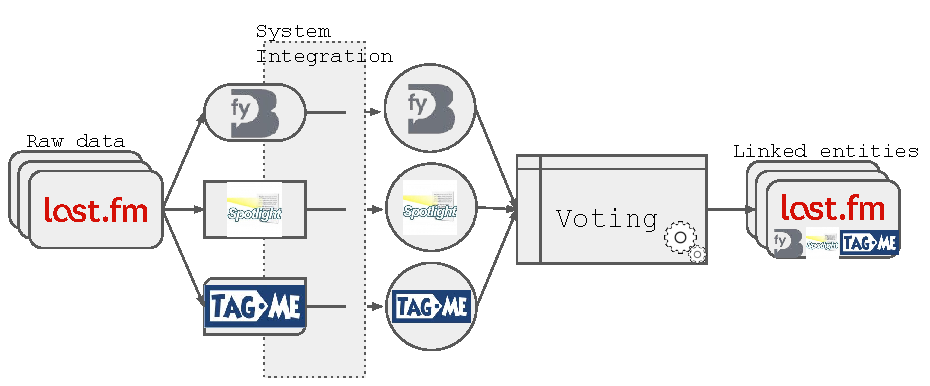
\includegraphics[height=3.25cm,width=8cm]{ch03_linking_pics/workflow.pdf}
  \caption{ELVIS Workflow}
  \label{fig:linking:workflow}
\end{figure}


\section{From \texttt{Last.fm} to \textsc{ELMD}}
\label{sec:linking:lastfm}

In what follows, we describe the original data gathered from \texttt{Last.fm}, and the process to apply the integration framework described in Section \ref{sec:linking:elvis}, in order to construct a highly precise benchmarking dataset for entity linking in the Music domain.


In \texttt{Last.fm}, users may add relevant biographical details to any artist's main page in the form of a \textit{wiki}. These edits are regularly moderated. Furthermore, artist biographies are often enriched with hyperlinks to other \texttt{Last.fm} Artist, Album, Song and Record Label pages, similarly as with Wikipedia hyperlinks. Our purpose is to leverage this meta-information to automatically construct a dataset of Music-specific annotated named entities.% and for evalauting the soundness of \textsc{ELVIS}.\\

We crawled artist biographies from \texttt{Last.fm} in March 2015, and gathered 13,000 artist biographies, which comprise 47,254 sentences with at least one hyperlink, amounting to a total of 92,930 links. These may be broken down as follows: (1) 64,873 hyperlinks referencing Artist pages; (2) 16,302 to Albums; (3) 8,275 to Song pages; and finally (4) 3,480 hyperlinks referencing Record Labels. This \textit{type} information is extracted thanks to the structure of each link's URL, as it includes in its path the category of the annotated entity. Consider, for example, the following sentence:

\begin{adjustwidth}{2.5em}{20pt}
\begin{center}
After their debut The Intelligence got signed to \textit{In the Red Records}.\\
\end{center}
\end{adjustwidth}


Here, we may infer that the entity \textit{In the Red Records} is a Record Label, thanks to its \texttt{Last.fm} URL: {\footnotesize{\texttt{http://www.last.fm/{\normalsize\textbf{label}}/In+the+Red+Records}}}. This information is extracted from the whole \texttt{Last.fm} corpus for those entities falling in one of the four \textit{musical categories} previously defined.

%%%\begin{figure}[h!]
%%%  \centering
%%%	\includegraphics[height=3.5cm]{elmd_creator.png}
%%%  \caption{Dataset creation.}
%%% \label{fig:linking:dataset_creator}
%%%\end{figure}

%After this extraction process, a first version of the dataset is built with the identified and categorized named entities.



\subsection{Data Enrichment}
\label{sec:linking:enrichment}

For the creation of the ELMD dataset, the crowdsourced annotations extracted from \texttt{Last.fm} biographies are combined with decisions made by \textsc{ELVIS} and its voting framework.\\%(see Figure~\ref{fig:linking:dataset_creator}).

Every entity mention annotated in the \texttt{Last.fm} corpus is a candidate to be included in \textsc{ELMD}. The challenge is to assign to each entity its correct DBpedia URI. We approach this problem by leveraging (1) The DBpedia URI assigned by \textsc{ELVIS}, (2) The \textit{agreement score} for that prediction, as well as (3) The \textit{type} information derived from the entity's \texttt{Last.fm} URL. Our intuition is that the higher the \textit{agreement score}, the more likely the prediction is to be correct. Likewise, we also hypothesize that if a linking decision made by \textsc{ELVIS} coincides in \textit{type} with the original \texttt{Last.fm} annotation, it is more likely to be correct. Since there is no direct mapping between \texttt{Last.fm} and DBpedia types, we manually set the type equivalences shown in Table \ref{tbl:linking:equivalence}.\\

Regarding the \textit{agreement score}, it corresponds to the number of systems that agreed in a decision (see \textbf{Score} column in Table \ref{tbl:linking:examples}). Note that an \textit{agreement score} of 1 may be caused either by cases in which only one system detected an entity mention, or when there is disagreement among systems, but one and only one of them coincides in \textit{type} with the original \texttt{Last.fm} annotation (last row in Table \ref{tbl:linking:examples}).

As for \textit{type equivalence}, this is a binary value (\textit{type-equivalent} or \textit{type-discrepant}) based on coinciding types between \texttt{Last.fm} URLs and \textsc{ELVIS} decisions.
%Note that agreement across systems within \textsc{ELVIS} is not considered (for instance, systems in \textsc{ELVIS} coincide in the example given in the third row of Table \ref{tbl:linking:examples}, but its \textit{type value} is set to \texttt{discrepant} since it does not match with the entity's \texttt{Last.fm} type).

%Additionally, when an entity is considered as disagreement by the agreement framework, but there is type equivalence with  one of the three entity linking systems, we change its confidence score from 0 to 1, and consider it also as a \textit{singleton} (there is an example of this special case in last row of Table~\ref{tbl:linking:examples}).\\

%To measure the usefulness of the type information, we divide the evaluation in two settings namely: (1) \textit{Type equivalence}, when the predicted and target entities share an equivalent type; and (2) \textit{Type nonequivalence}, when this is not the case. Note that for \textit{type nonequivalence} we consider both cases in which \texttt{Last.fm} and DBpedia types do not coincide, or when type information is absent in the DBpedia resource. 

%added to the ELMD dataset along with two features, namely its corresponding offset and \textit{type} information. Then, \textsc{ELVIS} is used to provide a linking between these entities and DBpedia as follows: For each detected entity, if the offset of the \texttt{Last.fm} annotation and an \textsc{ELVIS} prediction coincide, we leverage the \textit{confidence score} provided by the agreement among systems integrating \textsc{ELVIS} together with the entity type (see Table \ref{tbl:linking:equivalence}).% and use it as a confidence booster. %Therefore, there are two parameters that are used in the decision process, the confidence score and the type equivalence flag.


%provides a high precision linking between these entities and DBpedia. For each annotated entity, we obtain two important pieces of information: (1) \textsc{ELVIS} confidence score, which is obtained after applying the aforementioned \textit{agreement heuristics}; and (2) \textit{type} information, obtained from the original \texttt{Last.fm} data. 


%if there is an entity in the agreement output with the same offset, we analyze its confidence score and type information to decide whether to take its URI or not.
%We compare the type information gathered from DBpedia with the music categories inferred from the original \texttt{Last.fm} data 

%If our system considers both type information as equivalent, the 

%Additionally, in the type agreement setting, we consider as \textit{singleton} instead of disagreement, decisions cases in which 
%more than one system detects something in a text snippet, and they predict different entities, but 
%only one system predicts the correct type of the entity, giving to this entities a confidence score of 1.

%We acknowledge that, while this additional information may be helpful for enriching the \texttt{Last.fm} corpus, it does not reflect a realistic scenario in which we would perform entity linking on unseen data. 


%In addition to system agreements, we apply a music-specific heuristic exploiting music categories inferred from the original \texttt{Last.fm} data. Specifically, we use the \textit{music type} information provided through the rdf:type property of DBpedia resources as an agreement booster. This means that if the agreed URI contains a type that equivalent to the category of the candidate entity (see Table \ref{tbl:linking:equivalence}), we consider this as a case of \textit{type agreement}. For every level of system agreement, we differentiate the cases where there is type agreement from the other cases. In addition, when there is disagreement between systems, but only one of them detects an entity with type agreement, our confidence score is 1, like for singletons.

\begin{table}
\small
\centering
\def\arraystretch{1.2}
	\begin{tabular}{|l|l|}
\hline
\textbf{Last.fm type} & \textbf{DBpedia type} \\
\hline
Song & DBpedia:Song, DBpedia:Single, Yago:Song \\
Album & \parbox[t]{5cm}{DBpedia:Album, Yago:Album,\\ Schema:MusicAlbum} \\
Artist & \parbox[t]{5cm}{DBpedia:MusicalArtist, \\DBpedia:Band, Schema:MusicGroup, Yago:Musician, Yago:Creator, DBpedia:Artist} \\
Record Label & DBpedia:RecordLabel \\
\hline
	\end{tabular}
	\caption{Type equivalence}
	\label{tbl:linking:equivalence}
\end{table}

\begin{table*}[!t]
\scriptsize
\def\arraystretch{1.2}
\centering
	\begin{tabular}{| p{2cm} | c | L{1.8cm} | L{1.8cm} | L{1.5cm} | c | L{1cm} |}
\hline
\textbf{Context} & \textbf{Type} & \textbf{Tagme} & \textbf{Babelfy} & \textbf{Spotlight} & \textbf{Score} & \textbf{Type Eq.} \\
\hline
and the academic minimalism of \textbf{Steve Reich} & Artist &  Steve\_Reich (type:artist) & Steve\_Reich (type:artist) & Steve\_Reich (type:artist) & 3 & yes \\
\hline
The new album \textbf{Hypocrisy} followed shortly thereafter & Album & --- & Hypocrisy (type:band) & Hypocrisy (type:band) & 2 & no \\
\hline
The third album \textbf{Lucifer Songs}, opened new and unexpected doors & Album & --- & Lucifer\_Songs (type:album) & --- & 1 & yes \\
\hline
The band's debut album, \textbf{Cookies}, was released on 14 May 2007 & Album & HTTP\_cookie {\footnotesize{(type:unk)}} & Cookies (type:album) & --- & 1 & \parbox[t]{1cm}{\centering yes\\ (only\\ Babelfy)} \\
\hline
	\end{tabular}
	\caption{Agreement examples}
	\label{tbl:linking:examples}
\end{table*}

%\subsection{Unification Framework for Entity Linking}

%\subsection{Agreement-based Entity Linking Confidence}

\begin{figure}[!t]
  \centering
	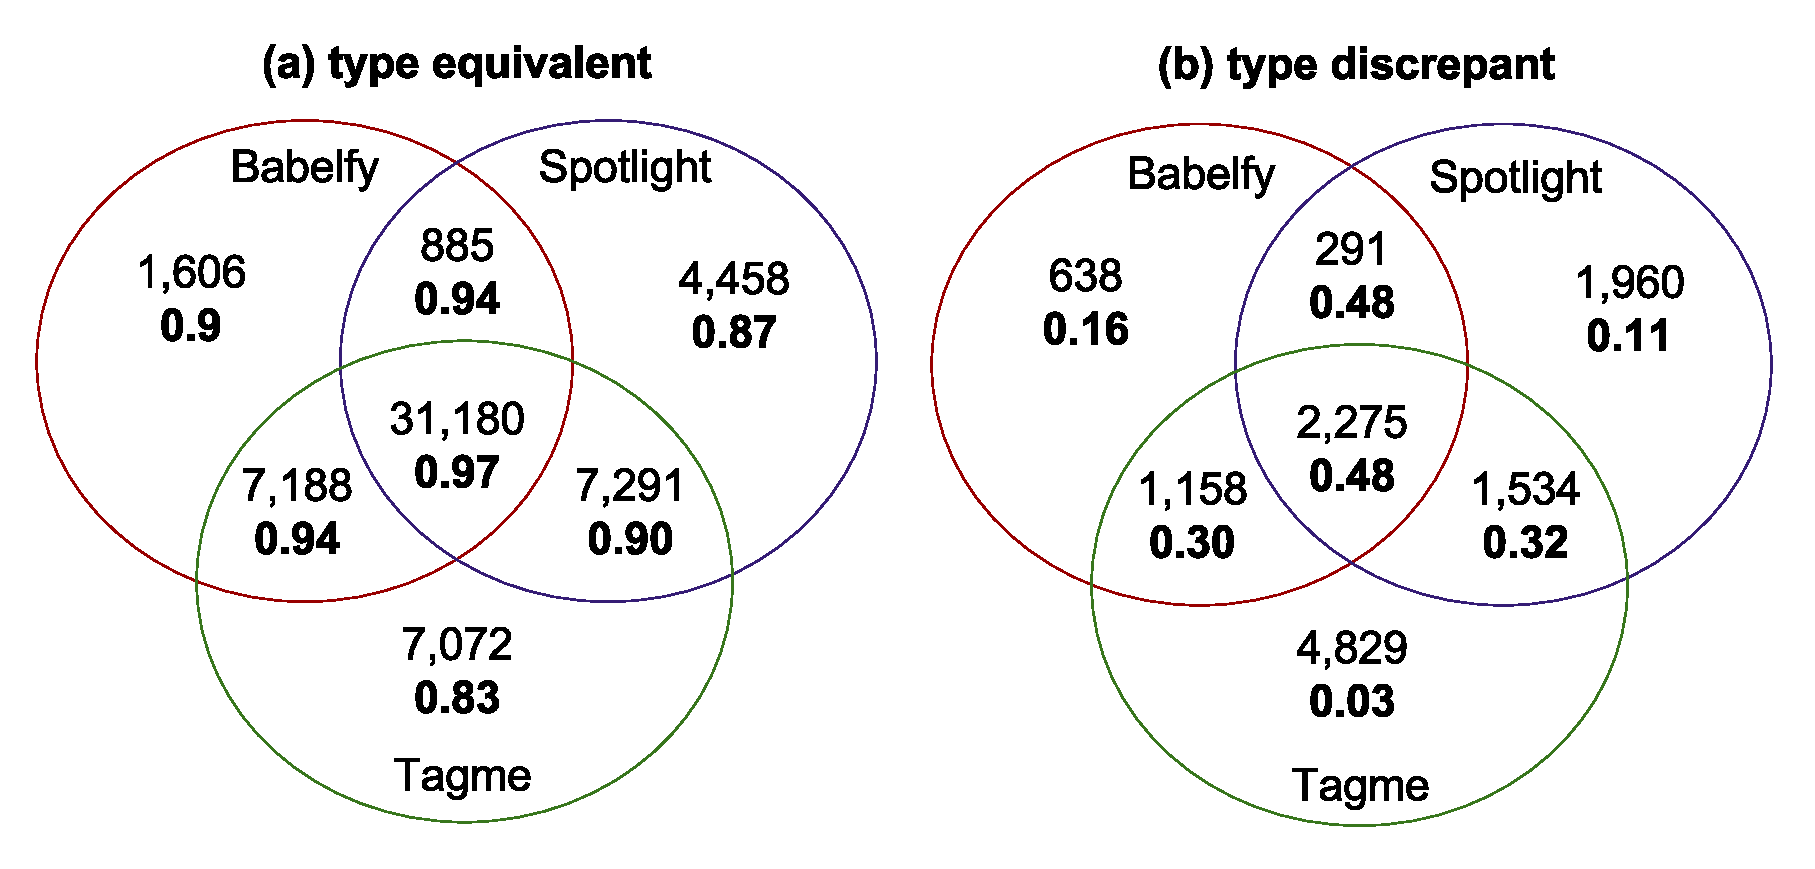
\includegraphics[width=\textwidth]{ch03_linking_pics/evaluation_both.eps}
  \caption{Number of entities and precision of the manual evaluation.  Note the major differences in Precision between \textit{type-equivalent} and \textit{type-discrepant} systems.}
  \label{fig:linking:agreement_typed}
\end{figure}

\begin{table}[ht!]
\centering
\def\arraystretch{1.2}
	\begin{tabular}{| c | c | c | c | c |}
\cline{2-4}
\multicolumn{1}{ c |  }{} & \textbf{Agreement} & \textbf{Precision} & \textbf{No. Entities} \\
\hline
\multirow{3}{*}{type-equivalent} & $=3$ & 0.97 & 31,180\\
&$\geq2$ & 0.96 & 46,544 \\
&$\geq1$ & 0.94 & 59,680 \\
\hline
%\multirow{3}{*}{type equivalence + type nonequivalence} & $=3$ & 0.94 & 33,455\\
\multirow{3}{*}{all} & $=3$ & 0.94 & 33,455\\
&$\geq2$ & 0.90 & 51,802\\
&$\geq1$ & 0.81 & 72.365\\
\hline
	\end{tabular}
	\caption[Precision and coverage]{Precision and number of entities with this value of precision. \textit{Type-equivalent} implies entities from the type-equivalent configuration only, whilst \textit{All} implies all entities regardless their type information.}
	\label{tbl:linking:results}
\end{table}

\section{Evaluation}
\label{sec:linking:eval}

Considering the different possibilities of agreement across the three systems integrating \textsc{ELVIS}, there are in total 7 possible configurations: 1 with \textbf{full agreement} (score$=3$); 3 with \textbf{partial agreement} (score $=2$); and 3 \textbf{singleton} configurations (score$=1$). Moreover, considering also the two possible values of \textit{type equivalence}, namely \texttt{equivalent} and \texttt{discrepant}, we have a total number of 14 configurations. Figure \ref{fig:linking:agreement_typed} provides a visual overview of these configurations, where we show both Precision scores for each configuration (in bold) in addition to the number of entities disambiguated with \textsc{ELVIS} in each case.

%Considering the two possible values of \textit{type agreement}, namely \texttt{equivalent} and \texttt{discrepant}, and the different possibilities of agreement across the systems integrating \textsc{ELVIS}, there are in total 14 possible configurations. These may be broken down into 7 configurations with \textit{type equivalence} and 7 configurations with \textit{type discrepancy}. These 7 configurations according to Entity Linking agreement: 1 \textbf{full agreement} configuration (score$=3$); 3 \textbf{partial agreement} configurations (score $=2$); and 3 \textbf{singleton} configurations  (score$=1$). Figure \ref{fig:linking:agreement_typed} provides a visual overview of these configurations, where we show both Precision scores for each configuration (in bold) in addition to the number of entities disambiguated with \textsc{ELVIS} in each case.\\

\begin{table*}[ht!]
\scriptsize
\small
\centering
\def\arraystretch{1.2}
	\begin{tabular}{|l|r|r|r|l|}
\hline
\textbf{Category} & \textbf{Annotations} & \textbf{Entities} & \textbf{Avg-words} & \textbf{Most frequent} \\
\hline
Song & 3,302 & 2,823 & 2.81 & Shine (6) \\
Album & 7,872 & 6,897 & 2.69 & Like Drawing Blood (6) \\
Artist & 46,337 & 17,535 & 1.88 & The Beatles (160) \\
Label & 2,169 & 815 & 1.94 & Sub Pop (33) \\
\hline
	\end{tabular}
	\caption{Statistics of the linked entities in ELMD. We report, for each \textit{musical category}, the total number of annotations linked to DBpedia, number of unique entities, average number of words per entity mention, and most frequently annotated entity (along with its frequency).}
	\label{tbl:linking:statistics}
\end{table*}

%(1 with \textbf{full agreement} 3, 3 with \textbf{partial agreement}, and 3 with confidence 1) with \textit{type equivalence}, and 7 with \textit{type nonequivalence}. These 14 combinations are illustrated in Figure~\ref{fig:linking:agreement_typed}. 

We evaluated 100 randomly selected entity samples (25 for each of the four Music categories we consider) from each one of the 14 possible configurations, and asked an eva\-luator with computational linguistics background to manually assess the correctness of the 1,400 predictions. From scores obtained from manual evaluation, we estimated Precision for the whole \textsc{ELMD} dataset with different ranges of \textit{agreement score} as well as two options \textit{type}-wise (see Table~\ref{tbl:linking:results}). The precision value for all the entities is computed proportionally according to the number of entities and the precision obtained in the manual evaluation for the \textit{type-equivalent} and \textit{type-discrepant} settings, hence these can be seen as Micro Average Precision numbers.

We observe that the \textit{type-equivalent} configuration yields much better Precision with only a slight tradeoff in terms of coverage. Therefore, we decided to select for the final \textsc{ELMD} dataset only those URIs stemming from a \textit{type-equivalent} setting where \textit{agreement score} is equal or greater to 1. This ensures a Precision of at least 0,94 in terms of entity linking. Moreover, a manual survey of false positives in the highest scoring setting (\textit{agreement score}$=3$ and \textit{type-equivalent}) showed that these are cases in which even a human annotator may not find it trivial to correctly find the correct entity to those entity mentions. One of these cases are those in which \textsc{ELVIS} is presented with and entity mention that on surface may refer to either an Artist or an Album named after the artist or band itself. An actual case of false positive in our evaluation dataset is the following sentence:
\begin{adjustwidth}{2.5em}{20pt}
\begin{center}
Her debut album , \textit{Kim Wilde}, (released on RAK records) came out in July 1981 and stayed in the U.K. album charts for 14 weeks, peaking at number 3 and getting much acclaim.
\end{center}
\end{adjustwidth}

Here, the entity \textit{Kim Wilde} should be disambiguated as the Album with the same name as the artist, but \textsc{ELVIS} incorrectly assigned the Artist's DBpedia URI: {\footnotesize{\texttt{dbpedia.org/resource/Kim\_Wilde}}}. In \textsc{ELMD} there are 50 cases where the same surface text is correctly linked to an Artist entity in some sentences, and to a Song entity in others. Similar ambiguous cases involving Artist and Album (148) and Song and Album (95) are correctly resolved by our system. These particularly challenging cases may be interesting for training Music specific entity linking algorithms.

Another interesting source of false positives comes between musical entities and equally named entities (not necessarily related to Music). In cases in which the latter are more popular in a reference KB, e.g. their associated node in the graph may have higher connectivity, may become prioritized by disambiguation entity linking algorithms that consider graph connectivity as a feature. Consider the following sentence:

\begin{adjustwidth}{2.5em}{20pt}
\begin{center}
He is becoming more and more in demand for his remixing skills; working for the likes of Justin Timberlake and Armand van Helden, and labels including \textit{Ministry Of Sound}, Defected and Intec, to name a just a few.
\end{center}
\end{adjustwidth}

Here, the entity \textit{Ministry of Sound} refers to a Record Label, a spin-off of the well-known club, which is the entity that was incorrectly assigned: {\footnotesize{\texttt{dbpedia.org/resource/Ministry\_of\_Sound}}}. 
Cases like this would require, first, to ensure that the different entities derived from \textit{Ministry of Sound} (such as the Record Label or a clothing brand of the same name) exist in a reference KB, and second, to exploit contextual information so that a correct decision is made.
A similar situation happens when song or album names may be confused with very common words or expressions (e.g. `Easy', `Stupid', `Sad song', `If', `Be there'). \textsc{ELMD} is rich in challenging cases like these.

%It would be very difficult, even for human annotators to obtain higher Precision. %[EJEMPLO DE CASO CONCRETO]

%We randomly selected a sample of 100 entities from each one of the 14 sets of entities defined in Figures~\ref{fig:linking:agreement_typed} and~\ref{fig:linking:agreement_nontyped}. In Figure~\ref{fig:linking:agreement_typed} are represented the entities with type agreement, whereas in Figure~\ref{fig:linking:agreement_nontyped} are represented the ones where the condition of agreement was not satisfied, whether because there is disagreement between the \texttt{Last.fm} type and the DBpedia type, or because there is not enough type information in the DBpedia resource. Thus, a total number of 1,400 entities were picked up, and the linking was manually evaluated by a linguist with annotation experience. From the precision levels obtained in the manual evaluation, we estimated the precision and recall of the different combinations of agreement for the whole dataset (see Table~\ref{tbl:linking:results}).

%Describe how evaluation data was generated

%Give numbers and discuss them (maybe include the figure by Sergio)

%Hihglight the fact that errors of type-A3 are actually impossible to detect even for a human.

\begin{figure}[h!]
  \centering
	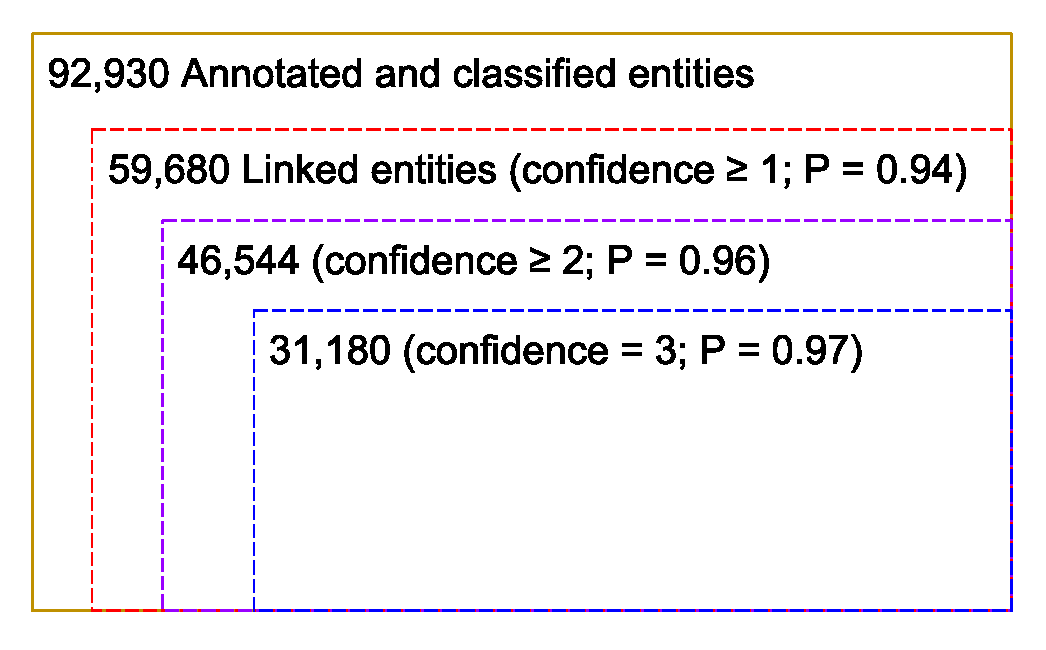
\includegraphics[width=8cm]{ch03_linking_pics/ELMD_Overview.eps}
  \caption{ELMD Overview. Number of entities, confidence score and precision values in different subsets of the dataset.}
  \label{fig:linking:elmd}
\end{figure}

\section{Extending ELMD}
\label{sec:linking:extending}

The number of links present in the \texttt{Last.fm} biographies is small compared to the size of the biographies. For instance, a link may have been added only once in a specific biography, even though the same entity is mentioned several times along the text. 
In addition, music information represented in DBpedia is not complete, as many existing artists, albums, and songs does not have a Wikipedia page. As a consequence of that, there are many annotated links in the biographies to \texttt{Last.fm} pages that does not have a corresponding DBpedia resource.
Therefore, to extend the coverage and the number of annotations of the \textsc{ELMD} dataset we applied the following processes. First, we take advantage of the fact that a large portion of \texttt{Last.fm} annotations have a direct mapping to MusicBrainz, and this information can be retrieved through the \texttt{Last.fm} API. Thus, in addition to the already available DBpedia links, MusicBrainz URLs are added to the annotations, when this information is available. Furthermore, existing annotations in every document are propagated, assuming they appear in a one-sense-per-discourse fashion \citep{gale1992one}. For example, if the text span \textit{The Beatles} is marked as an annotation in the first sentence of a document, and it appears again in the second sentence, but there is no annotation associated, an annotation is added. Finally, we look for mentions of the entity that constitutes the main theme of the biography, and annotate all its mentions within the biography, assuming unambiguity. The number of annotations and distinct entities after the extension process are reported in Table~\ref{tbl:linking:elmd2}. Note that MB has a coverage of 93.6\% over all the annotations, and 91.1\% over all distinct entities (see Table~\ref{tbl:linking:elmd2_percentage}).

\begin{table}[]
%\def\arraystretch{1.25}
\centering
\begin{tabular}{| l| r |r |}
\hline
& \textbf{Annotations} & \textbf{Entities} \\ \hline
All    & 144,593      & 63,902    \\ \hline
Artist & 112,524      & 39,131    \\ \hline
Album  & 18,701       & 15,064    \\ \hline
Song  & 9,203        & 7,832     \\ \hline
Label  & 4,165        & 1,875    
\\ \hline
\end{tabular}
\caption{Statistics of the extended ELMD corpus. \texttt{Annotations} refers to all distinct mentions or apparitions of an entity of its corresponding type, whereas the \texttt{Entities} column refers to the number of distinct entities of each type.}
\label{tbl:linking:elmd2}
\end{table}

\begin{table}[]
%\def\arraystretch{1.25}
\centering
\begin{tabular}{| l| r |r |}
\hline
& \textbf{Annotations} & \textbf{Entities} \\ \hline
DBpedia    & 58.6\%      & 49.1\%    \\ \hline
MusicBrainz & 93.6\%      & 91.1\%    \\ \hline
Both  & 57.2\%       & 47\%    \\ \hline
None & 5\%	& 9.2\% \\ \hline
\\ \hline
\end{tabular}
\caption{Percentage of linked entities in the extended ELMD corpus.}
\label{tbl:linking:elmd2_percentage}
\end{table}


\section{Gold Standard Dataset}
\label{sec:linking:gold}

We envision a wide range of potential applications for \textsc{ELMD}, such as acting as a training set for a named entity recognition or entity linking system, or as an evaluation benchmark. However, it suffers from two major problems that differentiate it from a gold standard dataset which undergous a full manual validation pass. First, although there is an important number of annotated entities, there are still many musical entities mentioned in \textsc{ELMD} texts that are not linked to any KB, nor even annotated. Second, as the dataset has been automatically generated, it is prune to errors, as we show in the evaluation in Section \ref{sec:linking:eval}. To tackle these issues, a subset of 200 documents from \textsc{ELMD} was manually annotated by a human expert. We asked the annotator to mark in each document all mentions of entities of the following types: \textit{Artist}, \textit{Album} and \textit{Song}. Record Label entities were discarded due to the low number of annotations present in the documents. In addition, the annotator manually searched for each entity in the MusicBrainz database. If it was present, the MusicBrainz URL was added to the annotation. The final number of annotations is shown in Table~\ref{tbl:linking:ELMDGold}.
This gold standard dataset has been used in the Task 3 of the third edition of the Open Knowledge Extraction Challenge, co-located with the Extended Semantic Web Conference (ESWC 2017) \citep{}.

\begin{table}[]
%\def\arraystretch{1.25}
\centering
\begin{tabular}{| l| r |r |}
\hline
& \textbf{Annotations} & \textbf{Entities} \\ \hline
All    & 5,184      & 2,803    \\ \hline
Artist & 3,828      & 1,926    \\ \hline
Album  & 860       & 693    \\ \hline
Song  & 496        & 184     \\ \hline
\end{tabular}
\caption{Statistics of the ELMDGold corpus. \texttt{Annotations} refers to all distinct mentions or apparitions of an entity of its corresponding type, whereas the \texttt{Entities} column refers to the number of distinct entities of each type.}
\label{tbl:linking:ELMDGold}
\end{table}


\section{Conclusion}
\label{sec:linking:conclusions}

In this chapter we have described several contributions related to the problem of recognizing and linking musical entities in naturally occurring text. First, for the task of entity linking, we have presented an integration framework called \textsc{ELVIS} which, based on a voting procedure which leverages decisions made by an arbitrary number of off-the-shelf entity linking systems, provides high confident entity disambiguations. Currently, \textsc{ELVIS} incorporates three state-of-the-art systems, namely DBpedia Spotlight, Tagme and Babelfy, and can be easily extended with additional systems. %The \textit{ELVIS} code is available at {\footnotesize{https://github.com/sergiooramas/elvis}}. 
Then, we have leveraged the potential of \textsc{ELVIS} for the creation of a novel benchmarking dataset for entity linking in the Music domain, called \textsc{ELMD}. This corpus comes from a collection of \texttt{Last.fm} artist biographies, and contains 47,254 sentences with 92,930 annotated and classified entity mentions. %(64,873 Artists, 16,302 Albums, 8,275 Songs and 3,480 Record Labels). 
%In addition, by setting up a higher confidence threshold it is possible to obtain a subset of \textsc{ELMD} that prioritize higher Precision by sacrificing Recall (see Figure~\ref{fig:linking:elmd}). 
From this set of entity mentions, 59,680 are linked to DBpedia (see Table~\ref{tbl:linking:statistics}), with a precision of at least 0,94 (see Figure~\ref{fig:linking:elmd}).
Moreover, we have extended the number of annotated entities in ELMD via several heuristics. Furthermore, in addition to the DBpedia linking, we successfully linked 93\% of the annotations to MusicBrainz by leveraging the \texttt{Last.fm} API.
Finally, we have manually annotated and linked to MusicBrainz a gold standard subset of 200 documents from ELMD, for its use within an entity linking challenge.
%\textit{ELVIS}\footnote{https://github.com/sergiooramas/elvis} source code and the different versions of \textsc{ELMD}\footnote{http://mtg.upf.edu/download/datasets/elmd} have been released.

\cleartorecto%!TEX root = ../thesis_a4.tex

\chapter[Automated Construction of Music Knowledge Bases][Automated Construction of MKBs]{Automated Construction of Music Knowledge Bases}
\label{sec:kb}

\section{Introduction}\label{sec:kb:introduction}

In this chapter, we present and evaluate an Information Extraction pipeline aimed at the construction of a Music Knowledge Base (MKB) entirely from scratch in an automated and unsupervised manner.
We combine a state-of-the-art Entity Linking tool and a linguistically motivated rule-based algorithm to extract semantic relations between entity pairs. 
Our method is able to generate a fully disambiguated MKB with entity mappings against DBpedia and MusicBrainz. All relations have a relation pattern derived from a Relation Extraction (Relation Extraction) procedure backed up by an algorithm that performs the following steps: (1) Morpho-syntactic rule-based \textit{filtering}; (2) Syntactic dependency-based \textit{clustering}; and (3) Relation \textit{weighting} based on statistical evidence. 

We validated our methodology on a large collection of documents in the music domain, obtained from \textit{songfacts.com}, a website that collects ``tidbits'' (short stories) about songs.
We carried out an intrinsic evaluation on each component of the algorithm, as well as an extrinsic evaluation which consists of a experiment on interpretation of music recommendations, where our automatically extracted MKB is used to provide explanations to song recommendations in \textit{natural language}.
Our experimental results indicate that our system is able to extract \textit{high quality} relations (Precision $>= 0.8$) as well as \textit{novel knowledge}. We unveil thousands of relations absent in both large-scale generic KBs, as well as in music specific resources. Moreover, the recommendation explanation experiment shows that explanations based on the newly extracted KB have a positive impact in user experience.

%We release the extracted MKB at several confidence levels, together with the evaluation data used in the experiments described in this chapter. The code for the complete Relation Extraction pipeline is also released as open source software under MIT license.

%The main contributions of this chapter are summarized as follows:
%\begin{itemize}
%    \item{We address for the fist time the problem of automatic construction of MKBs from plain text.}
%    \item{We put forward a novel approach for clustering relations, based on patterns derived from syntactic dependencies.}
%    \item{We present a new confidence measure over all extracted relations and demonstrate its discriminative power.}
%    \item{We showcase the utility of our method by creating a high quality MKB with \textit{novel knowledge}.}
%    \item{We demonstrate the usefulness of our automatically constructed MKB for providing explanations in natural language in the context of music recommendation.}
%\end{itemize}

%The work described in this chapter is a joint effort by the author of this thesis, and Luis Espinosa-Anke, both researchers in the UPF Department of Information Technologies. This collaboration is framed within the Maria de Maeztu strategic program, specifically in the Music Meets NLP project.

The rest of this chapter is organized as follows. In Section~\ref{sec:kb:method} we describe step by step the proposed methodology for relation extraction. Then, in Section~\ref{sec:kb:exp} we illustrate the gathered dataset and the outcome of the relation extraction process. The results of our evaluation are reported in Section~\ref{sec:kb:experiments}, and the chapter ends with a discussion about our findings.

\section{Method}
\label{sec:kb:method}

We propose a comprehensive pipeline that extracts a full-fledged MKB taking as input raw text collections. The experiments we report in this chapter are the result of applying our method to a dataset of plain text extracted from the Songfacts\footnote{\url{http://www.songfacts.com}} website (see Section~\ref{sec:kb:exp:dataset}). This is a well suited resource both for KB construction and as a testebed for Relation Extraction due to its specificity. Essentially, Songfacts documents, while not being as rigid as encyclopedic text or newswire text, remain well-formed, sentences make sense, and there is no need for \textit{ad-hoc} preprocessing (as it is required in social networks, e.g. Twitter). Our method, however, can be ported with little effort to music-related corpora of different registers.

\subsection{Notation}

Our method focuses on the extraction of semantic relations between pairs of linked entities (e.g. \textit{Born in the USA}$_{dbr}$, \textit{Bruce Springsteen}$_{dbr}$\footnote{We use the \textit{dbr} subscript to refer to disambiguated entities linked to DBpedia resources.}), which are in turn associated to specific entity types (e.g. \textit{Album}, \textit{MusicalArtist}). In our KB, a relation $r$ is defined by the tuple $\langle \textbf{\textit{e}}{_\textbf{\textit{d}}},
\textbf{\textit{e}}{_\textbf{\textit{r}}},
\boldsymbol\upsilon{_\textbf{\textit{d}}},
\boldsymbol\upsilon{_\textbf{\textit{r}}},
\textbf{\textit{p}}, \textbf{\textit{c}}\rangle$, where \textbf{\textit{d}} and \textbf{\textit{r}} refer to domain and range positions, $\textbf{\textit{e}}{_\textbf{\textit{d}}}$ and $\textbf{\textit{e}}{_\textbf{\textit{r}}}$ to the entities involved in the relation, $\boldsymbol\upsilon{_\textbf{\textit{d}}}$ and
$\boldsymbol\upsilon{_\textbf{\textit{r}}}$ to their associated entity types, \textbf{\textit{p}} to a relation pattern, and \textbf{\textit{c}} to a cluster pattern.  
A relation pattern is a relation label that may be used in one or several relations (e.g \textit{was recorded by frontman}, \textit{was recorded by singer/songwriter}). Relation patterns with similar semantic and syntactic characteristics may be grouped into cluster patterns (e.g. \textit{was recorded by}). 
$\mathcal{R}$ denotes the set of all extracted relations included in the KB.
For each $r \in \mathcal{R}$, triples of different nature can be constructed by arbitrarily combining elements in $r$.

\begin{itemize}
    \item $t_\textbf{\textit{p}}: \langle \textbf{\textit{e}}{_\textbf{\textit{d}}},\textbf{\textit{p}},\textbf{\textit{e}}{_\textbf{\textit{r}}} \rangle$ , e.g. \{\textit{Born in the USA}$_{dbr}$ - \textit{was recorded by frontman} - \textit{Bruce Springsteen}$_{dbr}$\}.
    \item $t_\textbf{\textit{c}}: \langle \textbf{\textit{e}}{_\textbf{\textit{d}}},\textbf{\textit{c}},\textbf{\textit{e}}{_\textbf{\textit{r}}} \rangle$ , e.g. \{\textit{Born in the USA}$_{dbr}$ - \textit{was recorded by} - \textit{Bruce Springsteen}$_{dbr}$\}.
    \item $\tau_\textbf{\textit{p}}: \langle \boldsymbol\upsilon{_\textbf{\textit{d}}},\textbf{\textit{p}},\boldsymbol\upsilon{_\textbf{\textit{r}}} \rangle$ , e.g. \{\textit{Album} - \textit{was recorded by frontman} - \textit{MusicalArtist}\}.
    \item $\tau_\textbf{\textit{c}}: \langle \boldsymbol\upsilon{_\textbf{\textit{d}}},\textbf{\textit{c}},\boldsymbol\upsilon{_\textbf{\textit{r}}} \rangle$ , e.g. \{\textit{Album} - \textit{was recorded by} - \textit{MusicalArtist}\}.
\end{itemize}

Finally, different subsets of $\mathcal{R}$ may be constructed by selectively filtering all $r \in \mathcal{R}$.  

\begin{itemize}
    \item $\mathcal{R}_{p} = \{r_1^p, ... r_n^p\}$ All relations with a specific relation pattern $p$.
    \item $\mathcal{R}_{c} = \{r_1^c, ... r_n^c\}$ All relations with a specific cluster pattern $c$.
    \item $\mathcal{R}_{\boldsymbol\tau{_\textbf{\textit{p}}}} = \{r_1^{\tau{_p}}, ... r_n^{\tau{_p}}\}$ All relations with a specific relation pattern, and domain and range entity types.
    \item $\mathcal{R}_{\boldsymbol\tau{_\textbf{\textit{c}}}} = \{r_1^{\tau{_c}}, ... r_n^{\tau{_c}}\}$ All relations with a specific cluster pattern, and domain and range entity types.
\end{itemize}

In what follows, we describe a method for acquiring new entities, types and relations, and combining them in a meaningful way for KB construction.


\subsection{Morphosyntactic Preprocessing}\label{sec:kb:method:preprocessing}

Our morphosyntactic preprocessing module takes as input a collection of text documents in the music domain. First, sentence splitting and tokenization is carried out thanks to the \textit{Stanford NLP tokenizer}\footnote{\url{http://nlp.stanford.edu/software/tokenizer.shtml}}. 
Next, a dependency parse tree is obtained via the MATE Parser, described in \cite{Bohnet2010}. We justify the use of the latter because of the richness of its tagset, as well as performance in terms of accuracy and speed, which were appropriate for the task at hand.

In a dependency tree, each node includes information, at least and depending of the model and the language, about surface and lemmatized forms, along with its part-of-speech. Each edge in the tree is labeled with a dependency relation such as \textit{subject} or \textit{noun modifier} (an example is shown in Figure ~\ref{fig:kb:sampletree}).


\begin{figure}[!htb]
\centering
\begin{dependency}
\begin{deptext}[column sep=.0cm]
NN \& NN \& VBD \& VBN \& IN \& NNP \& NNP \\
\textbf{Sweet} \& \textbf{Freedom} \& was \& written \& by \& \textbf{Rod} \& \textbf{Temperton} \\
\end{deptext}

\deproot[edge height=10ex]{3}{root}

\depedge[edge style={ultra thick, dotted}]{3}{2}{SBJ}
\depedge[edge style={ultra thick, dotted}]{3}{4}{VC}
\depedge[edge style={ultra thick, dotted}]{2}{1}{NAME}

\depedge[edge style={ultra thick, dotted}]{4}{5}{LGS}
\depedge[edge style={ultra thick, dotted}]{5}{7}{PMOD}
\depedge[edge style={ultra thick, dotted}]{7}{6}{NMOD}

\end{dependency}
\vspace*{-5mm}
\caption{Example sentence with dependency parsing tree.}
\label{fig:kb:sampletree}
\end{figure}


\subsection{Semantic Processing: Entity Linking}
\label{sec:kb:method:entitylinking}

Entity Linking acts as a semantic bridge between plain text and a reference knowledge inventory. %While there are a number of popular Entity Linking systems which are not bound to any domain or discipline, 
As explained in Chapter~\ref{sec:linking}, there is no benchmark of Entity Linking systems in the music domain, so we do not know \textit{a priori} how well the different systems behave in music corpora. Musical entities may raise a plethora of challenges, derived mostly from ambiguity and polysemy. For example, an album may have the same name as the band who recorded it (e.g. \textit{Weezer} the band and their first album). Moreover, an artist, a song or an album may have words or expressions much more common in another domain or area of knowledge (e.g. \textit{Berlin, The Who}). Thus, the choice of the best Entity Linking algorithm or off-the-shelf tool(s) is crucial, as potential errors may propagate throughout the different modules and hinder considerably the quality of the resulting KB.

Among the available Entity Linking systems we considered, namely TagMe \citep{Ferraginaetal2010}, Babelfy \citep{Moroetal2014} and DBpedia Spotlight \citep{Mendes2011}, we opted for the latter, as it has shown to be the least prone to errors in our corpus (further details are provided in Section~\ref{sec:kb:experiments:qualityentitylinking}).

\subsubsection{Adding Co-references}

In the music domain, prototypical factoid documents such as artist biographies, album reviews, or song tidbits, normally refer to one specific entity. Based on this observation, we may exploit co-referential pronouns and \textit{resource-specific co-references}, replacing them by the name of the reported entity.
A similar approach is used in \cite{Voskarides2015}, where the frequency of pronouns ``he'' and ``she'' is computed in every document (Wikipedia articles in this specific case) to determine the entity's gender, and then, these pronouns are replaced by the entity title. %Similarly, in \cite{Oramas2014}, a gender identifier web service is used to determine the gender of subjects in artist biographies as part of a Relation Extraction pipeline.

We have observed an exploitable \textit{resource-specific co-reference} in music reviews, where terms like ``this album'' or ``the song'' can be replaced by the document's title. In the dataset used for the experiments (see Section~\ref{sec:kb:exp:dataset}), the expressions ``this song'' and ``the song'' are replaced with the name of the song as it appears in the document, and disambiguated with the URI of the entity they unequivocally refer to.

Co-reference resolution is a difficult and crucial task in NLP, affecting tasks such as Information Extraction \citep{Soon2001} or document summarization \citep{saggion2004multi}. It is also sensitive to the domain in which it appears (see, for instance, the case of the patents domain \citep{Bouayad2014}). We acknolwedge the difficulty of this task. However, while addressing this problem in its entirety is out of the scope of this chapter, the described strategy allows us to increase coverage of entity mentions while maintaining a high precision.



\subsubsection{Type Filtering}
\label{sec:kb:typefiltering}

In DBpedia, most resources are associated with one or more types via the \texttt{rdf:type} property. In addition, among the different types present in DBpedia (coming from the DBpedia ontology, Yago types, or \texttt{schema.org}), the DBpedia ontology provides a relatively small and tidy taxonomy of 685 classes based on Wikipedia infoboxes. Other KBs such as Yago or Freebase have their own ontological structure, which is in general broader and noisier. MusicBrainz, in contrast, has a very narrow set of entity types. 

This type information can be exploited in order to narrow down the set of allowed types for a given candidate and its potential annotations. In this way, we ensure that all entities will be, at least, related to the music domain. Restricting the search space to types such as Artist or Song reduces considerably the number of errors derived from cross-domain ambiguity. For instance, the Entity Linking system detects a substantial amount of entities whose DBpedia type is \textit{FictionalCharacter}, which are in most of the cases misleading song titles or band names with fictional characters of the same name. This situation is observed also with other types of entities such as \textit{Athlete}, \textit{Species} or \textit{Disease}.

Depending on the envisioned application of the KB resulting from our pipeline, the predefined set of entity types may vary. In our case we restricted them to Musical Artists, Other Artists, Songs, Albums, Genres, Films and Record Labels. In Table~\ref{tbl:kb:type_mapping} we present the mapping between the DBpedia ontology, MusicBrainz entity types and our selected set of types.

\begin{table}[]
\scriptsize
\centering
	\begin{tabular}{ l l l }
	\hline
\textbf{Our MKB} & \textbf{DBpedia ontology} & \textbf{MusicBrainz} \\
	\hline
\multirow{4}{*}{MusicalArtist} & Person/Artist/MusicalArtist & \multirow{4}{*}{Artist}\\ 
& Organization/Band & \\ 
& Writer/MusicComposer & \\ 
& Writer/SongWriter & \\
	\hline
\multirow{2}{*}{OtherArtist} & Person/Artist ($\neg$ MusicalArtist) & \multirow{2}{*}{---} \\
& Person/Writer($\neg$ MusicComposer \& $\neg$ SongWriter) & \\
    \hline
Album & Work/MusicalWork/Album & Release \\
    \hline
\multirow{2}{*}{Song} & Work/MusicalWork/Song & Recording \\
& Work/MusicalWork/Single & Work \\
    \hline
Genre & TopicalConcept/Genre & --- \\
    \hline
Film & Work/Film & --- \\
    \hline
RecordLabel & Agent/Organization/Company/RecordLabel & Label \\
    \hline
	\end{tabular}
	\caption{Type mapping.}
	\label{tbl:kb:type_mapping}
\end{table}
%

\subsection{Syntactic Semantic Integration}
\label{sec:kb:method:syntsemint}

The information obtained from the syntactic and semantic processes is combined into a graph representation of the sentence. For each music entity identified during the semantic processing step (Section~\ref{sec:kb:method:entitylinking}), all nodes in the dependency tree with a correspondence with an entity mention are collapsed into one single node: \textit{Sweet} and \textit{Freedom} into \textit{Seet Freedom (Album)}, and \textit{Rod} and \textit{Temperton} into \textit{Rod Temperton (Artist)}. Figure ~\ref{fig:kb:sampletree_combined} shows the resulting syntactic-semantic representation of a sentence.

\begin{figure}[!htb]
\centering
\begin{dependency}
\begin{deptext}[column sep=.0cm]
\textbf{Album} \& VBD \& VBN \& IN \& \textbf{Person} \\
\textbf{Sweet Freedom} \& was \& written \& by \& \textbf{Rod Temperton} \\
\end{deptext}

\deproot[edge height=10ex]{4}{root}

\depedge[edge style={ultra thick, dotted}]{2}{1}{SBJ}
\depedge[edge style={ultra thick, dotted}]{2}{3}{VC}
\depedge[edge style={ultra thick, dotted}]{3}{4}{LGS}
\depedge[edge style={ultra thick, dotted}]{4}{5}{PMOD}

\end{dependency}
\vspace*{-5mm}
\caption{Semantic integration on syntactic dependencies.}
\label{fig:kb:sampletree_combined}
\end{figure}


\subsection{Relation Extraction and Filtering}
\label{sec:kb:method:re-filtering}

Our approach to Relation Extraction is lightweight, unsupervised and rule-based. Having syntactic and semantic information available, potential relations between entities may be discovered by traversing the dependency tree.
Two entities in such tree are considered to be related if there is a path between them that does not contain any other entity in between, and does not contain parentheses. If there is more than one path, we consider only the shortest path as the most representative path of the relation.

Our method encodes a relation pattern between two entities as all words in the shortest path between them. In the example provided in Figure ~\ref{fig:kb:sampletree_combined}, the shortest path between \emph{Sweet Freedom} and \emph{Rod Temperton} contains the words \textit{was}, \textit{written} and \textit{by}.

While Relation Extraction via shortest path in syntactic trees is common practice in the literature \citep{DelliBovietal2015b,MoroandNavigli2012,Nakasholeetal2012}, not all shortest paths are valid, and incorrect relations may be extracted from overly long and syntactically complex sentences. We aim at surmounting these problems by defining three filtering heuristics over surface forms (\textit{lemma-paths}), part-of-speach patterns (\textit{pos-paths}), and labels of syntactic dependencies (\textit{dependency-paths}).

First, we filter out all relations with reporting verbs (e.g. ``say'', ``tell'' or ``express'') in the lemma-path (see the full list of banned lemmas in Table~\ref{tbl:kb:rules}). The intuition being that sentences with these verbs are by definition syntactically complex, and semantic relations in them may not be encoded via shortest paths. We illustrate this with the following sample sentence, where the relation extracted with syntactic tree traversal by means of shortest path would be incorrect:

\begin{itemize}
\item[] \textbf{Sentence:} \texttt{Nile Rodgers} \textit{told} NME that the first album he bought was Impressions by \texttt{John Coltrane}.
\item[] \textbf{Relation}: \texttt{nile\_rodgers} told that was impressions by \texttt{john\_coltrane}
\end{itemize}

Second, we only selected relations where the syntactic function that connects in the dependency-path the fist entity with the first word of the relation pattern is a subject (which may be preceded by a nominal modifier or an apposition), a direct or indirect object, a predicative complement or a verb chain (see the full list of allowed patterns in Table~\ref{tbl:kb:rules}). When this condition holds, the relation is considered \textit{valid}. If the above condition does not hold, an extra validation step is applied over the pos-path in order to capture relations without verbs, which seem to be idiosyncratic of the music domain, e.g. $\langle e_d, \mbox{\texttt{frontman of}}, e_r \rangle$, $\langle e_d, \mbox{\texttt{drummer}}, e_r \rangle$, or $\langle e_d, \mbox{\texttt{guitarist and singer}}, e_r \rangle$ (see the full list of allowed pos patterns in Table~\ref{tbl:kb:rules}).

\begin{table}[]
\scriptsize
\centering
    \begin{tabular}{ c l p{5cm} }
    \hline
    Filtering Heuristics & Description & Patterns \\
    \hline
    lemma-paths & banned lemmas & say, tell, speak, explain, express, mention, inform, thank, ask, admit\\
    \hline
    dependency-paths & allowed start patterns & PRD, VC, SBJ, NMOD SBJ, OBJ, APPO SBJ \\
    \hline
    pos-paths & special allowed patterns & NN, NN NN, NNS, NN CC NN, NN IN, IN NN \\
    \hline
    \end{tabular}
    \caption{Complete set of patterns used in the filtering heuristics}
    \label{tbl:kb:rules}
\end{table}

\subsection{Dependency-Based Loose Clustering}
\label{sec:kb:method:clustering}

In this section we describe a simple but powerful clustering algorithm aimed at reducing the number of relation patterns in the KB. %noise in our relation patterns inventory.% inventory $\mathcal{P}$.

Let us consider the following three relation patterns: (1) \textit{was written by blunt producer}, (2) \textit{was written by singer/producer}, and (3) \textit{was written by manager and guitarist}. Intuitively, these three relation patterns seem to be semantically similar, and if all of them were expressed as \textit{was written by}, the original meaning would not be lost, and the set of relations would become more compact.

This observation, which we found to occur quite frequently, motivated the inclusion of a \textit{dependency-based loose clustering} module. First, we perform a second run of dependency parsing over all relation patterns extracted by our system, aiming at discovering their root node. We apply this second run because the root of the original sentence does not need to correspond with the relation pattern's root. Then, our algorithm considers all possible paths from the root to every leaf node of the relation pattern dependency tree, and selects the path that complies with a predefined syntactic constraint (e.g. a sequence of verbs plus adverb or preposition, or adverb plus nominal and preposition modifiers) based on regular expressions of syntactic labels. The sequence of tokens that matches this regular expression constitutes the cluster pattern. The complete set of defined regular expressions is reported in Table~\ref{tbl:kb:expressions}. %included in the released source code.

\begin{table}[]
\scriptsize
\centering
    \begin{tabular}{ l}
    \hline
    Regular Expressions \\
    \hline
    \^(VC)+\textbackslash s*(DEP|LGS|LOC|TMP) \\
    \^(VC)+\textbackslash s+(ADV)\\s*(PMOD|NMOD|AMOD)* \\
    \^(DEP|LGS|LOC|TMP) \\
    \^(APPO)\textbackslash s+(LGS) \\
    \^(SBJ)\textbackslash s*(PMOD|NMOD|AMOD|ADV) \\
    \^(OBJ)\textbackslash s*(PMOD|NMOD|DEP) \\
    \^(ADV) \\
    \^(NMOD|PRT|PMOD) \\
    \hline
    \end{tabular}
    \caption{Complete set of regular expressions for dependency paths in cluster patterns.}
    \label{tbl:kb:expressions}
\end{table}

As an illustrative case, consider the extracted relation pattern \textit{is track was released on label} from the sentence \textit{\texttt{Sing Out The Song} is the 7th track on Wishbone Four which was released in the UK May 1973 on the \texttt{MCA} label}. After re-parsing the relation pattern, we obtain the parse tree shown in Figure \ref{fig:kb:parsedpattern} and a cluster pattern over those nodes in the dependency tree that satisfy one of the regular expressions crafted in the aforementioned syntactic constraint. Finally, the obtained relation is \textit{\texttt{Sing\_out\_the\_song} was released on label \texttt{MCA}}.

\begin{figure}[!htb]
\centering
\begin{dependency}
\begin{deptext}[column sep=.5cm]
is \& track \& was \& released \& on \& label \\
\end{deptext}

\deproot[edge height=10ex]{3}{root}

\depedge[edge style={}]{3}{2}{SBJ}
\depedge[edge style={ultra thick}]{3}{4}{VC}
\depedge[edge style={}]{2}{1}{NMOD}

\depedge[edge style={ultra thick}]{4}{5}{ADV}
\depedge[edge style={ultra thick}]{5}{6}{PMOD}

\end{dependency}
\vspace*{-5mm}
\caption{Example of a parsed relation pattern $p \in \mathcal{P}$ and a valid cluster pattern (bold).}
\label{fig:kb:parsedpattern}
\end{figure}


Filtering out spurious information in OIE following similar approaches has proven effective while not being computationally expensive \citep{Fader2011}.

Ours is a \textit{loose clustering} method because it does not enforce a pattern to fully match all rules, but rather allows partial matching. This module provides an enrichment of all $r \in \mathcal{R}$ such that $r = \langle e_d, e_r, \upsilon_d, \upsilon_r, p, c\rangle$, where $c$ is the cluster pattern derived from the relation pattern $p$. A relation cluster is the set of all relations with the same cluster pattern, and is denoted as $\mathcal{R}_c$. 


\subsection{Scoring}
\label{sec:kb:method:scoring}

So far, our approach has identified entity mentions in text and has linked them in meaningful relations, filtering out those that did not comply with predefined linguistic rules. We incorporate one additional factor $score(r)$ that takes into account statistical evidence computed over $\mathcal{R}$. It has three main components, which we flesh out as follows.

We hypothesize that the relevance of a cluster may be inferred by the number and proportion of triples it encodes, and whether these are evenly distributed. 
Our metric encompasses a combination of three different components. First, we focus on the \textit{degree of specificity} of the relation cluster, as previous work has demonstrated that this can contribute to Information Extraction pipelines \citep{DelliBovietal2015}. Second, we analyze \textit{intrinsic features} of the relation pattern, such as frequency, length and fluency. Finally, we incorporate a \textit{smoothing factor}, namely the proportion of the related typed cluster pattern in the cluster.

\begin{table}[]
\scriptsize
	\begin{tabular}{ | l | l | l | }
	\hline
\textbf{Cluster pattern $c$} & \textbf{Typed cluster pattern $ \tau_\textbf{\textit{c}}$} & \textbf{Relation triples $t_\textbf{\textit{p}}$} \\
\hline
\multirow{10}{*}{\textit{was written by}} & \multirow{3}{*}{S \textit{was written by} MA} & s1 \textit{was writen by artist} ma1 \\
\cline{3-3}
 &  & s2 \textit{was written by composer} ma2 \\
\cline{3-3}
 &  & s3 \textit{was written by singer} ma2 \\
\cline{3-3}
&  & s4 \textit{was writen by} ma1 \\
 \cline{3-3}
&  & s5 \textit{was written by frontman} ma3 \\
\cline{2-3}
& \multirow{3}{*}{A \textit{was written by} MA} & a1 \textit{was written by frontman} ma3 \\
 \cline{3-3}
&  & a2 \textit{was written by guitarist} ma1 \\
\cline{3-3}
&  & a3 \textit{was written by artist} ma2 \\
\cline{3-3}
&  & a4 \textit{was written by frontman} ma5 \\
    \hline
	\end{tabular}
	\caption[Example of a relation cluster.]{Example of a relation cluster $\mathcal{R}_c$, where $c = \mbox{\textit{was written by}}$. \textit{S} refers to Song, \textit{MA} to MusicalArtist and \textit{A} to Album types, whilst \textit{sX} refers to Song, \textit{maX} to MusicalArtist and \textit{aX} to Album entities.}
	\label{tbl:kb:example_grouping}
\end{table}

A cluster $\mathcal{R}_c$ may be decomposed into a set of typed cluster patterns $\tau_c$ (see Table ~\ref{tbl:kb:example_grouping}). The intuition behind the specificity measure of a cluster is that clusters with one prominent $\tau_c$ are more specific, i.e. they are largely used for encoding one specific type of relations. One example of this would be \textit{performed with}, which enforces a relation to include MusicalArtists on both the domain and range sides. Thus, we define $\mathcal{L}_c$ as the list of cardinalities (number of triples) of every typed cluster pattern $\tau_c \in \mathcal{R}_c$, being $\mathcal{L}_c = \{|\mathcal{R}_{\tau_c^1}|,...,|\mathcal{R}_{\tau_c^n}|\}$. We define the specificity measure as the variance of $\mathcal{L}$, expressed as $s(\mathcal{R}_c) = var(\mathcal{L}_c)$.

Furthermore, we consider a \textit{relation's fluency} metric, which is aimed at capturing its comprehensibility. Simply put, the more the sentence's original word order is preserved in the relation pattern, the more understandable it should be. This metric is introduced due to the fact that word order is lost after modelling text under a dependency grammar framework, and so we design a \textit{penalty measure} over the number of jumps needed to reconstruct the original ordered word sequence. Let $k$ be the number of tokens in the relation pattern, $w_i$ the $ith$ word in the pattern, and $h(w_i)$ a function that returns the correspondent word index in the original sentence, we put forward a fluency measure $f$ defined as:

\begin{equation}
f(p) = \frac{\sum_{i=1}^{k} \alpha | h(w_i) - h(w_{i-1}) |}{k}
\end{equation}

where $\alpha=2$ if $h(w_{i-1}) > h(w_i)$ and $\alpha=1$ otherwise. Note that higher values of $f$ means low fluency. For instance, for the relation pattern \textit{is hit for} the score would be much higher than a mixed-up order relation pattern such as \textit{joined because added were and hit}, which would have a very high $f$.  

Finally, the global confidence measure for each relation $r \in R$ is expressed as follows:

\begin{equation}
score(r) = \left({s(\mathcal{R}_c) + \frac{|\mathcal{R}_p|}{|p|+2^{f(p)}}}\right) \times {\frac{|\mathcal{R}_{\tau_c}|}{|\mathcal{R}_c|}}
\end{equation}

As an illustrative example of the measure, the score of a relation with the typed cluster pattern $\langle$Song, \textit{was released on}, RecordLabel$\rangle$, will have a much higher score than a relation whose typed cluster pattern is $\langle$Album, \textit{was released on}, MusicalArtist$\rangle$. This latter pattern is incorrect, probably due to a disambiguation error in the Entity Linking step. Relations like this show the type of errors which our proposed confidence score is expected to consider for pruning.



\section{Experimental Setup}\label{sec:kb:exp}

In this section, we describe our experimental setting. We refer first to the source raw corpus, and second to the resulting KBs as output of different branches of our approach.


\subsection{Source dataset}\label{sec:kb:exp:dataset}

Songfacts\footnote{\url{http://www.songfacts.com}} is an online database that collects, stores and provides facts, stories and trivia about songs. These are collaboratively written by registered users, and reviewed by the website staff. It contains information about more than 30,000 songs from nearly 6,000 artists. This information may refer to what the song is about, who wrote it, who produced it, who collaborated with whom or who directed the video. These texts are rich sources of information not only for well-known music facts, but also for music-specific trivia, as in the following sample sentence (about David Bowie's \textit{Space Oddity}): ``Bowie wrote this song after seeing the 1968 Stanley Kubrick movie 2001: A Space Odyssey".

We crawled the Songfacts website in mid-January 2014. Then, for each song article, we performed a mapping between the song and its MusicBrainz recording ID, using the MusicBrainz Search API. We successfully mapped 27,655 songs.

The described methdology was run over the 27,655 documents in the Songfacts corpus, which amounts to 306,398 sentences. After the Semantic Processing step, we obtained 202,767 linked entities (8,880 for \textit{Albums}, 3,136 \textit{Record Labels}, 74,908 \textit{Songs}, 107,253 \textit{Musical Artists}, 1,760 \textit{Genre} labels, 3,467 for \textit{Other Artist}, and 3,363 for \textit{Film}). There were 48,122 sentences with at least two entities, and it is on this subset where we apply our Relation Extraction pipeline.


\subsection{Extracted Knowledge Bases}
\label{sec:kb:exp:learnedkbs}

Our aim is to assess to what extent each of the modules integrating our approach contributes to the quality of the resulting KB. After executing the whole pipeline, we generate two \textit{extracted} KBs (\textsc{KBSF}-ft and \textsc{KBSF}-th), two \textit{baseline} KBs (\textsc{KBSF}-co and \textsc{KBSF}-raw), and a \textit{competitor} KB (\textsc{KBSF}-rv). 

The \textit{extracted} KBs are the result of applying the Relation Extraction method to the Songfacts dataset under different conditions. \textsc{KBSF}-ft is derived from applying the Relation Extraction pipeline entirely, and \textsc{KBSF}-th comes from a selection of all triples in \textsc{KBSF}-ft with a confidence score above a certain threshold. To determine the best threshold to prune \textsc{KBSF}-ft, we aimed at maximizing the number of triples and at the same time minimizing the number of relation patterns. Our intuition is that less patterns means a tidier KB. Therefore, we computed the percentage of triples and relation patterns from \textsc{KBSF}-ft that remain in a pruned KB, whose triples have a score greater than a certain threshold $\theta$. We computed these percentages for every $\theta$ value ranging from 0 to 1 in bins of 0.01 (see Figure \ref{fig:kb:th}). Our goal was to discover the $\theta$ value which maximizes the distance between the amount of triples and the amount of relation patterns in a pruned KB. After confirming a maximized difference with $\theta=0.05$, we created \textsc{KBSF}-th, whose triples have a score greater than or equal to 0.05. In this pruned KB, we have 36.56\% of \textsc{KBSF}-ft triples, with only 12.52\% of its relation patterns.

\begin{figure}[!htp]
\centerline{\framebox{
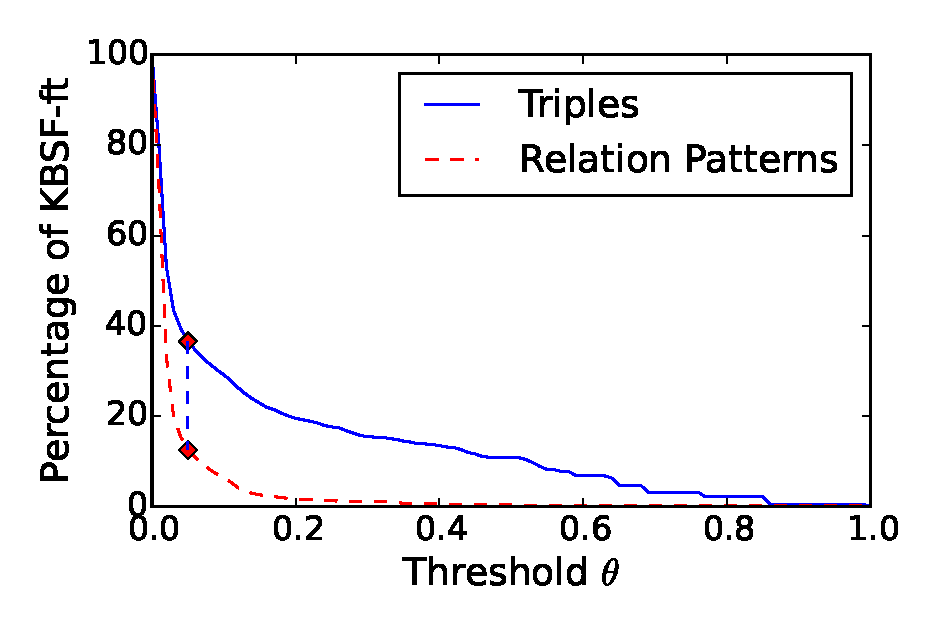
\includegraphics[width=8cm]{ch04_kbconstruction_pics/threshold.eps}}}
\caption[Percentage of triples and relation patterns from \textsc{KBSF}-ft.]{Percentage of triples and relation patterns from \textsc{KBSF}-ft that remain after pruning at different values of $\theta$. Maximum distance at $\theta=0.05$.}
\label{fig:kb:th}
\end{figure}

In addition, we created two baseline KBs for evaluation purposes. \textsc{KBSF}-co is a baseline which consists of simple entity co-occurrence. More specifically, if two entities are mentioned in the same sentence, an unlabelled triple that anchors them is added to the KB. In addition, \textsc{KBSF}-raw was created following the Relation Extraction pipeline, but without applying the filtering process described in Section~\ref{sec:kb:method:re-filtering}. Finally, \textsc{KBSF}-rv constitutes the competitor KB, and is built as follows: After running \textsc{ReVerb} \citep{Fader2011}, a state-of-the-art Relation Extraction system, over the Songfacts dataset, we search coinciding relations, at both domain and range positions, that include entity mentions identified in our disambiguation step. These relations are included in KBSF-rv. Statistics about the five KBs are reported in Table \ref{tab:kbs}.

\begin{table*}[ht!]
\scriptsize
\centering
	\begin{tabular}{ | c | c | c | c | c | }
	\hline
	\textbf{KB} & \textbf{Entities} & \textbf{Triples} & \textbf{Relation Patterns} & \textbf{Cluster Patterns} \\
	\hline
	\textsc{KBSF}-ft & 20,744 & 32,055 & 20,438 & 14,481 \\
	\textsc{KBSF}-th & 10,977 & 11,720 & 2,484 & 828 \\
	\hline
	\textsc{KBSF}-co & 30,671 & 113,561 & --- & --- \\
	\textsc{KBSF}-raw & 29,280 & 71,517 & 47,089 & 32,712 \\
	\hline
	\textsc{KBSF}-rv & 9,255 & 7,532 & 2,830 & --- \\
	\hline
	\end{tabular}
	\caption{Statistics of all the extracted KBs}
	\label{tab:kbs}
\end{table*}


\section{Experiments}
\label{sec:kb:experiments}

\subsection{Quality of Entity Linking}
\label{sec:kb:experiments:qualityentitylinking}

%We mentioned in Section~\ref{sec:kb:method:entitylinking} the lacking of both music-specific Entity Linking tools as well as benchmarking datasets. For this reason, 
In this section, we performed a set of experiments to select the best-suited Entity Linking tool for our task, among some of the best known and reputed. Specifically, we perform evaluation experiments on DBpedia Spotlight, TagMe and Babelfy. 

%Let us briefly describe each of them: 

%\begin{itemize}
%    \item \textbf{Babelfy} \cite{Moroetal2014} A graph-based system for Entity Linking and Word Sense Disambiguation. It operates on the back of BabelNet, which serves as a reference sense inventory.
%    \item \textbf{Tagme} \cite{Ferraginaetal2010} An Entity Linking automatic annotator which matches terms with Wikipedia hyperlink texts and disambiguates them using both the in-link graph and the page datasets. It incorporates a context-aware pruning step.
%    \item \textbf{DBpedia Spotlight} \cite{Mendes2011} Automatically identifies entity mentions in free text, linking each match with its corresponding DBpedia URI.
%\end{itemize}

As stated in Chapter~\ref{sec:linking}, most Entity Linking systems \textit{speak their own language}. Since their output is heterogeneous in format, performing a comparison between them is not straightforward. In order to evaluate the aforementioned Entity Linking systems, we used \textsc{ELVIS} (see Section~\ref{sec:linking:elvis}), an Entity Linking integration tool which provides a common output for different Entity Linking system.

In addition, we created a dataset of annotated musical entities based on our corpus of documents, and applied both quantitative and qualitative evaluations in order to verify which system performs better with musical entities, and is more suitable for our task.



\subsubsection{Evaluation Data}

We created an \textit{ad-hoc} ground truth dataset to evaluate the different Entity Linking systems in an excerpt of the corpus where they will be later applied, the Songfacts dataset (Section~\ref{sec:kb:exp:dataset}). In this corpus, each document univocously refers to one single song. In addition, we have information about artist and song names at our disposal. We used this information to obtain the MusicBrainz ID for songs and artists. In MusicBrainz, artist and song items sometimes have information about their equivalent Wikipedia page. We leveraged this information, when available, to obtain their corresponding DBpedia URIs. Finally, we obtained a mapping with DBpedia of 7,691 songs and 3,670 artists. From the DBpedia data about each song, we gathered their corresponding album name and URI, if available, obtaining information of about 2,092 albums. Then, for every document, we looked for exact string matches of the reported song, and its related album and artist names. Every detected entity is thus annotated with its DBpedia URI. At the end of this process, the newly created evaluation dataset contains 6,052 documents where 17,583 sentences are annotated with the following entities: 5,981 Song, 12,137 Artist and 1,722 Album entities. As mentioned in Section~\ref{sec:kb:method:entitylinking}, there are typical cases of ambiguity in musical entities where songs, artists and albums can potentially share the same name. Therefore, we manually corrected the entities detected in 212 documents where this kind of ambiguity was present.


\subsubsection{Entity Linking Evaluation}

\begin{table}[]
\scriptsize
\centering
	\begin{tabular}{ c c c c c c c c c c }
	\hline
& \multicolumn{2}{c}{Album} & \multicolumn{2}{c}{Artist} & \multicolumn{2}{c}{Song} & \multicolumn{3}{c}{Macro Average}  \\
\hline
	& Prec & Rec & Prec & Rec & Prec & Rec & Prec & Rec & F-measure \\
	\hline
Babelfy & 0.93 & 0.28 & 0.98 & 0.55 & 0.96 & 0.31 & 0.96 & 0.38 & 0.54 \\
Tagme & 0.75 & 0.69 & 0.97 & 0.77 & 0.65 & 0.71 & 0.79 & 0.72 & \textbf{0.76} \\
Spotlight & 0.80 & 0.52 & 0.94 & 0.83 & 0.59 & 0.42 & 0.78 & 0.59 & 0.67 \\
\hline
	\end{tabular}
	\caption{Precision and recall of the entity linking systems considered.}
	\label{tbl:kb:res_categories}
\end{table}

\begin{figure}[!htp]
\centerline{\framebox{
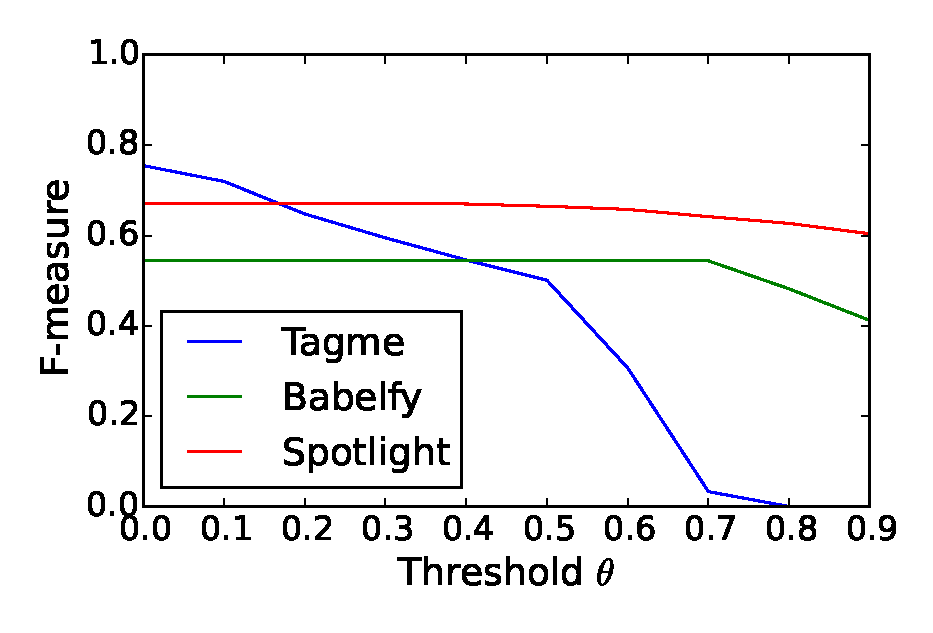
\includegraphics[width=8cm]{ch04_kbconstruction_pics/threshold_el.eps}}}
\caption[F-measure of the entity linking systems at different thresholds.]{F-measure of the entity linking systems at different confidence thresholds.}
\label{fig:kb:confidence_el}
\end{figure}

The three Entity Linking systems under review provide their own confidence measure. Hence, we evaluated their output filtering out the entities with a confidence measure below to a certain threshold $\theta$. We run the evaluation for different values of $\theta$, ranging from 0 to 0.9 in bins of 0.1. After evaluating on the ground truth dataset, the best results in terms of F-measure were obtained by all the systems at $\theta = 0$ (see Figure ~\ref{fig:kb:confidence_el}), which means that there is no need to apply any filtering process based on the Entity Linking system own confidence score. Detailed results on the run of every system at $\theta = 0$ are shown in Table~\ref{tbl:kb:res_categories}. We used macro-average Precision and Recall measures, i.e. we averaged their values from the three sets of entities.

We may conclude from these results that Babelfy is the system with highest Precision on musical entities. However, its recall is lower than the other systems under consideration, and specifically with respect to Tagme, which in turn, shows much lower precision. DBpedia Spotlight, on the other hand, achieves a similar precision score as Tagme, but with a slightly lower recall. 

This evaluation experiment is only focused on measuring the precision in the annotation of entities present in the ground truth dataset. However, since all possible entities in a document may be not annotated, we also report on specific types of false positives which emerged during a qualitative inspection of classification results. For example, a frequent error that is not being evaluated concerns cases in which a text span not annotated in the ground truth is identified incorrectly as an entity by any system. Therefore, to complement the evaluation, we listed the most frequently identified entities by each system (see Table~\ref{tbl:kb:top_entities}). As we can see, Babelfy and Tagme are misidentifying common words as entities very frequently, whereas DBpedia Spotlight is not doing so. 
These errors may propagate to the rest of the Relation Extraction pipeline, penalizing the accuracy of the final KB.
Although a filtering process could be applied to filter out misidentified entities by computing their tf-idf score in each document, we opted for using DBpedia Spotlight, as it has shown pretty good performance, its output does not require any further processing, and it is released as open source, which means that there are no limitations on the number of queries.

\begin{table*}[ht!]
%\tiny
\scriptsize
\centering
	\begin{tabular}{  c c c c }
	\hline
System & Song & Album & Artist \\
	\hline
\multirow{5}{*}{Babelfy} & \textbf{Carey} & \textbf{Debut} & John\_Lennon \\
& \textbf{Stephen} & \textbf{Song\_For} & Eminem \\
& \textbf{Rap\_Song} & \textbf{Sort\_Of} & Paul\_McCartney \\
& \textbf{Singing\_This\_Song} & \textbf{First\_Song} & Bob\_Dylan \\
& \textbf{A\_Day\_in\_the\_Lif}e & \textbf{Debut\_Album} & Drake \\
	\hline
\multirow{5}{*}{Tagme} & \textbf{The\_Word} & \textbf{Up!} & John\_Lennon \\
& \textbf{The\_End} & \textbf{When\_We\_On} & \textbf{The\_Notorious\_B.I.G.} \\
& \textbf{If} & \textbf{U}p & \textbf{Do} \\
& \textbf{Once} & \textbf{Together} & Paul\_McCartney \\
& \textbf{For\_You} & \textbf{By\_the\_Way} & \textbf{Neil\_Young} \\
	\hline
\multirow{5}{*}{Spotlight} & Sexy\_Sadie &  The\_Wall & Madonna \\
& Helter\_Skelter & Let\_It\_Be & Eminem \\
& Cleveland\_Rocks & Born\_This\_Way & Rihanna \\
& Stairway\_to\_Heaven & Thriller & John\_Lennon \\
& Minnie\_the\_Moocher & Robyn & Britney\_Spears \\
	\hline
	\end{tabular}
	\caption[Top-5 most frequent entities by type and tool.]{Top-5 most frequent entities by type and tool. Disambiguation errors appear in bold. }
	\label{tbl:kb:top_entities}
\end{table*}


\subsection{Quality of Relations}
\label{sec:kb:experiments:qualityofrelations}

\begin{figure}[t]
   \centering
    \begin{subfigure}[b]{0.49\textwidth}
        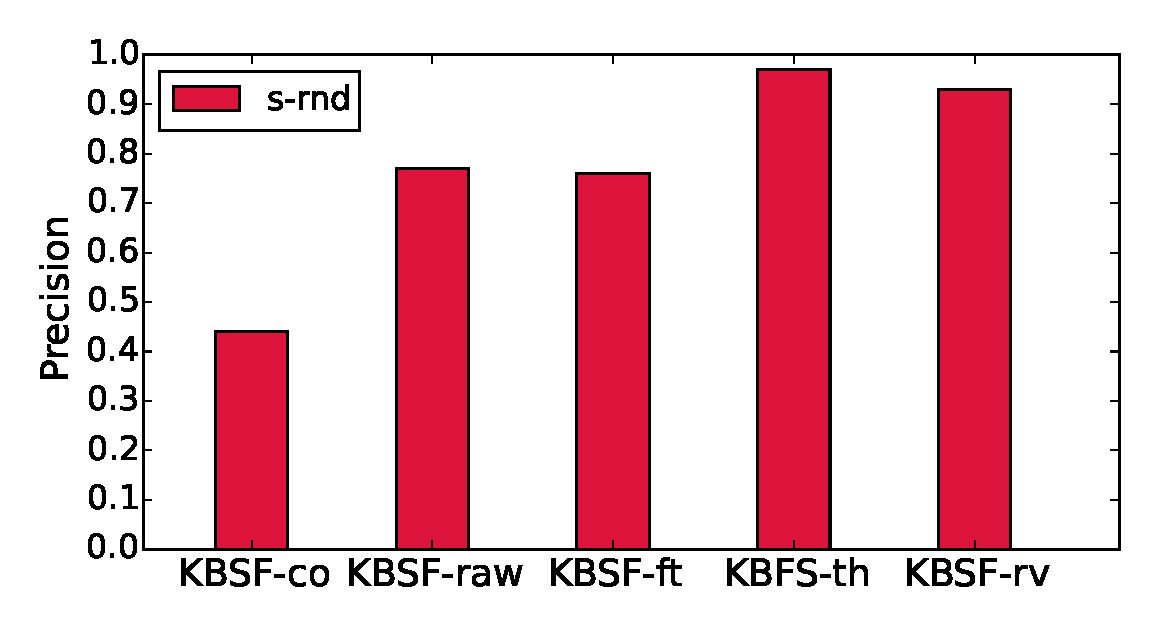
\includegraphics[width=\textwidth]{ch04_kbconstruction_pics/s-rnd100.eps}
        \caption{In sentence}
        \label{fig:kb:p_sentence}
    \end{subfigure}
    \begin{subfigure}[b]{0.49\textwidth}
        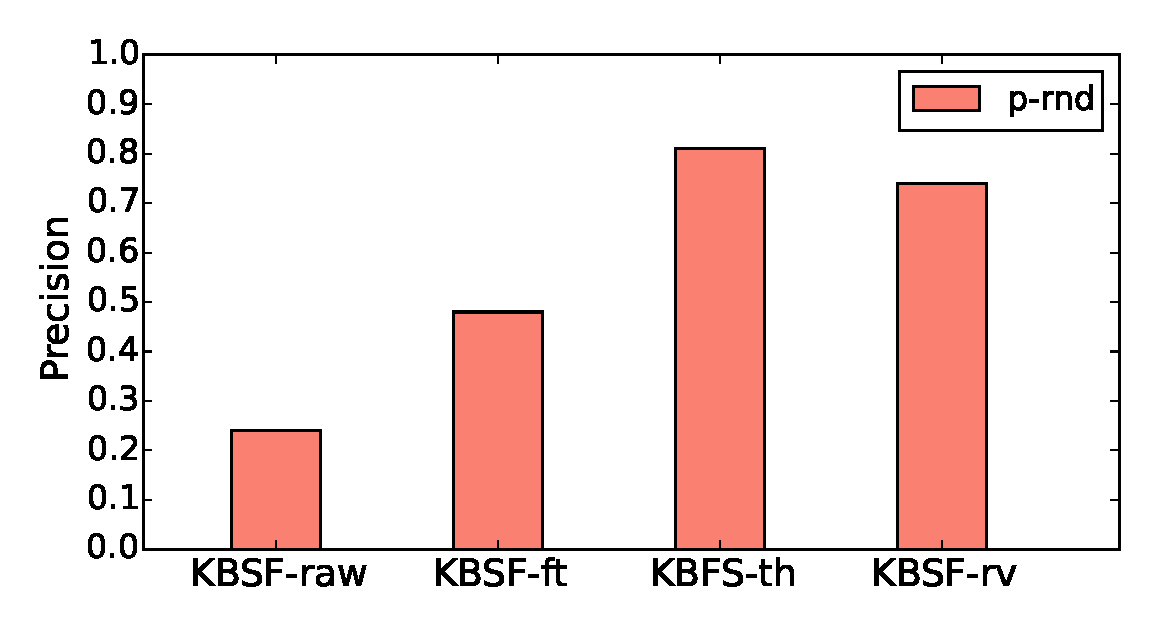
\includegraphics[width=\textwidth]{ch04_kbconstruction_pics/p-rnd100.eps}
        \caption{Relation patterns}
        \label{fig:kb:p_patterns}
    \end{subfigure}
    \begin{subfigure}[b]{0.49\textwidth}
        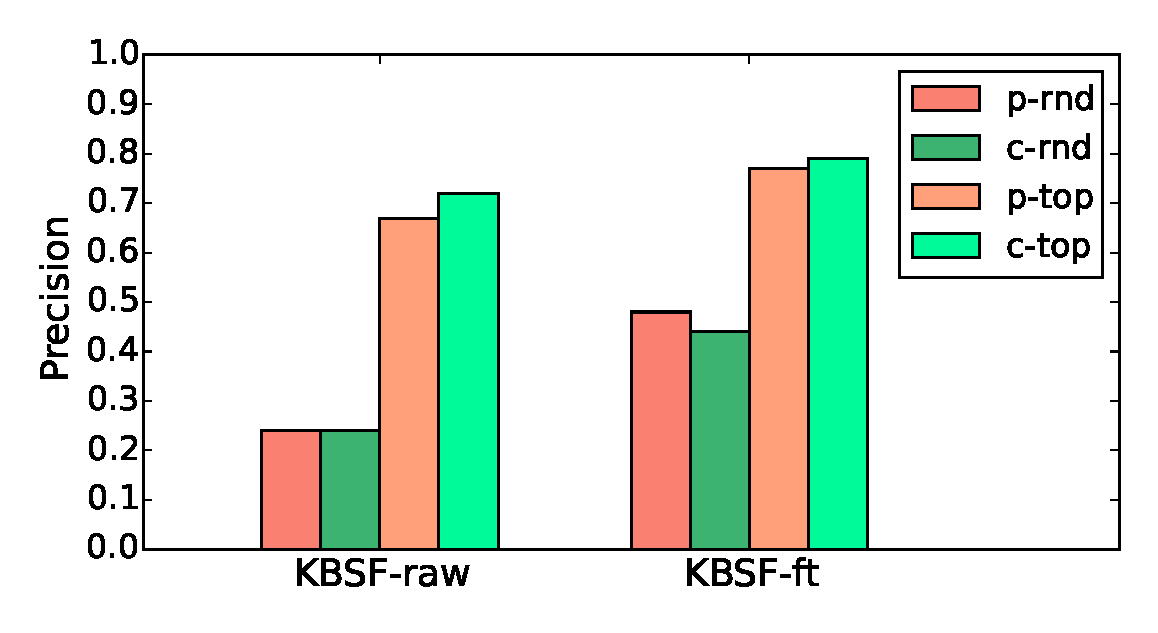
\includegraphics[width=\textwidth]{ch04_kbconstruction_pics/eval_p_c.eps}
        \caption{Patterns and clusters}
        \label{fig:kb:p_clusters}
    \end{subfigure}
    \caption[Precision of relations.]{Precision of relations at sentence (\textit{s}), relation pattern (\textit{p}) and cluster pattern (\textit{c}) levels in top (\textit{top}) and random (\textit{rnd}) samples of relations}\label{fig:kb:eval_relations}
\end{figure}

Relation Extraction evaluation is not trivial, as semantic relations between entities may vary in terms of correctness over time. Also, correct relations may be linguistically flawed, i.e. not fluent. Previous approaches assessed automatically extracted relations in terms of correctness according to human judgment \citep{Fader2011,Mausam2012}. Additionally, a finer grained analysis is carried out in \cite{Bankoetal2007}, adding a prior step in which relations are judged as being \textit{concrete} or \textit{abstract}.

In this chapter, we made use of extensive human input and asked two experts in Computational Linguistics to evaluate the \textit{top 100} scoring relations as yielded by our weighting policy (Section \ref{sec:kb:method:scoring}), as well as a random sample of 100 relations. This was done for all the KBs produced by our pipeline and for \textsc{KBSF}-rv. Cohen's kappa coefficient ranged from 0.60 to 0.81, which is generally considered as \textit{substantial} agreement.


In Figures \ref{fig:kb:p_sentence} and \ref{fig:kb:p_patterns}, where we compare random samples from each KB, we observe a gradual improvement of the quality of relations as the different modules of our implementation are incorporated. The difference between these figures is that in the former, a relation is deemed correct if it has extracted a relation \textit{expressed in the original sentence}, whereas the latter figure reports numbers on whether the extracted relation pattern was correct, i.e. if it \textit{meant} the same as it was intended in the source sentence. We may infer from the difference of precision between \textsc{KBSF-co} and \textsc{KBSF-raw} in Figure~\ref{fig:kb:p_sentence} that co-occurrence between entities does not guarantee an explicit relation, whereas the presence of a path between two entities over a sentence dependency tree, without any other entity mention in between, generally suggests a monsemous and unambiguous relation.

It is remarkable how well \textsc{ReVerb} performs (Figure \ref{fig:kb:p_patterns}), only being surpassed by the KB resulting from the complete implementation described in this chapter. We note that the good results of the \textsc{ReVerb} extractor are also due to the semantic processing of our system, which is forcing \textsc{ReVerb} to select good candidates as relation arguments. Recall that the difference between \textsc{KBSF}-ft and \textsc{KBSC}-th is the inclusion of the \textit{scoring} module, and the increase in Precision confirms that incorporating \textit{statistical evidence contributes to better relations}.

This is further confirmed in the results showcased in Figure \ref{fig:kb:p_clusters}, where we provide a comparison between top 100 relations according to our ranking policy against a random sample. Note that \textit{in all KBs, highly scoring relations are more often marked as correct}, which constitutes additional support for the contribution of the scoring module. Together with the quality of the relation pattern, this figure shows the quality of the cluster pattern associated with the evaluated relations. We observe that cluster patterns inferred in our clustering module have similar quality than relation patterns in the random sample, and slightly better in the top 100 sample. This result implies that the scoring module is rewarding good clusters.

\subsection{Coverage of the Extracted Knowledge Base}
\label{sec:kb:experiments:coverage}

With this experiment, we aim to compare the coverage of music relations in our final KB with respect to other resources with human intervention, such as DBpedia, MusicBrainz, and with automatically created resources. For the latter, we considered \textsc{DefIE} \citep{DelliBovietal2015b} as our closest competitor due to several methodological similarities (dependency parsing, Entity Linking and Relation Extraction over shortest paths). 

We selected all triples in \textsc{KBSF}-th whose domain and range entities could be mapped to both DBpedia and MusicBrainz. %As our extracted KB has only MusicBrainz ID of entities of types MusicalArtist and Song, the set of triples to evaluate is restricted to relations between them. 
In addition, since entities in \textsc{DefIE} are disambiguated against BabelNet ids, we mapped all DBpedia uris to their corresponding BabelNet id. After mapping the entities, we obtained a subset of 3,633 triples. From here, we selected all possible pairs of domain-range entities present in these triples, and retrieved from the other KBs all triples involving the same pairs, and counted them.
The procedure to do so on DBpedia was via SPARQL queries.
From the retrieved triples after querying, we discarded those with predicate \textit{wikiPageWikiLink}, as this predicate means an unlabeled relation. By contrast, the mapping with MusicBrainz was not trivial. MusicBrainz is not a KB of triples, but a relational database. Entities are stored in tables, and relations between entities are represented in a set of tables of relations, having one table for each possible relation. %The entities in the studied set of triples were only of type MusicalArtist and Song. However, 
In addition, an entity of type Song in \textsc{KBSF}-th can be related to either a Recording or a Work entity in MusicBrainz (see Section~\ref{sec:kb:method:typefiltering}). Therefore, for the analysis of relations involving a Song entity, we obtained the equivalent Recording and Work MusicBrainz entities, and looked up relations where any of them where present.

Mapping results are shown in Table~\ref{tbl:kb:coverage}. Let us highlight the fact that most semantic relations encoded in \textsc{KBSF}-th are novel, as they were not found in any of the other resources we compared against. In the overlapping cases, most of the times the relation labels were semantically equivalent, and often the relation label of \textsc{KBSF}-th triples was more specific than the ones retrieved from other KBs (e.g. \textit{frontman} vs. \textit{member of})

\begin{table}[]
%\scriptsize
\centering
	\begin{tabular}{ c c c c c }
	\hline
	& KBSF-th & MusicBrainz & DBpedia & DefIE \\
	\hline
	Relation instances & 3,633 & 1,535 & 1,240 & 456 \\
%	Relation patterns & 746 & 24 & 32 &  \\
	\hline
	\end{tabular}
	\caption[Number of triples with labeled relations in the different KBs.]{Number of triples with labeled relations in the different KBs for the same set of domain-range entity pairs.}
	\label{tbl:kb:coverage}
\end{table}


\subsection{Interpretation of Music Recommendations}
\label{sec:kb:experiments:recommendation}

The main aim of this experiment is to evaluate the suitability of \textsc{KBSF}-th to explain relations between songs, and study their impact on user's experience in music recommendation. 
Since our aim is not to measure the performance of a recommender system, we implemented a baseline recommender approach. Recommendations are based on the concept of song similarity, which exploits the graph-based structure of our KB. Maximal common subgraph score is computed between the item neighborhood graphs of every song. This methodology for entity similarity is fully described in Section~\ref{sec:similarity:method:sim:mcs} of Chapter~\ref{sec:similarity}. Once the similarity scores are computed, similar songs are ranked.


We designed the experiment as an online survey, where the participant is first asked to select 5 songs from different artists of his/her choice. From each selected song, the system randomly selects 3 recommendations among the list of its top-10 most similar songs. One of them is shown together with an explanation in natural language (the source text), another with an explanation based on relation patterns, and finally the third one appears without explanation.
Participants can listen to all songs with an embedded player. After listening to the recommendation and reading the explanation attached to it, participants were asked to rate each recommendation from 1 to 5 (1 being worst), and to mention whether they were familiar or not with the recommended songs (see Figure~\ref{fig:kb:recommender}).


The experiment involved 35 participants, 28 males and 7 females, ranging from 26 to 38 years old and with different musical background and listening habits. Most of the participants said that they had previous experience with recommendation systems. 
A total of 525 answers (corresponding to individual song recommendations) were collected. In 38\% of the cases, the user was familiar with the recommended songs.

The average rating of recommendations with natural language explanations is slightly higher (3.20$\pm$1.29) than recommendations without explanations (3.08$\pm$1.35), or with explanations based on relation labels (3.04$\pm$1.34). In addition, for musically educated individuals, recommendations of unfamiliar songs, whether accompanied with or without explanations, have similar average rating (2.87 and 2.95 respectively). However, for untrained users, recommendations with explanations have a remarkable higher average rating (2.93) than without them (2.36). Thus, we can infer that the introduction of explanations in recommender systems improves the user experience of musically untrained subjects when discovering songs.

We also asked the subjects to select among a set of adjectives those that better described the recommendation experience. The general trend was to rate positively the experiment. Most users rated the experience as \textit{enjoyable} (40\%), followed by \textit{useful} (31\%) and enriching (29\%). Negativity was much lower in general, with \textit{confusing} being the most voted (17\%), followed by \textit{complicated} and \textit{too geeky} (8\% in both cases). This suggests that the introduction of explanations generated from our MKB in the recommendations was in general a satisfactory experience to users.


\begin{figure}[!htp]
\centerline{
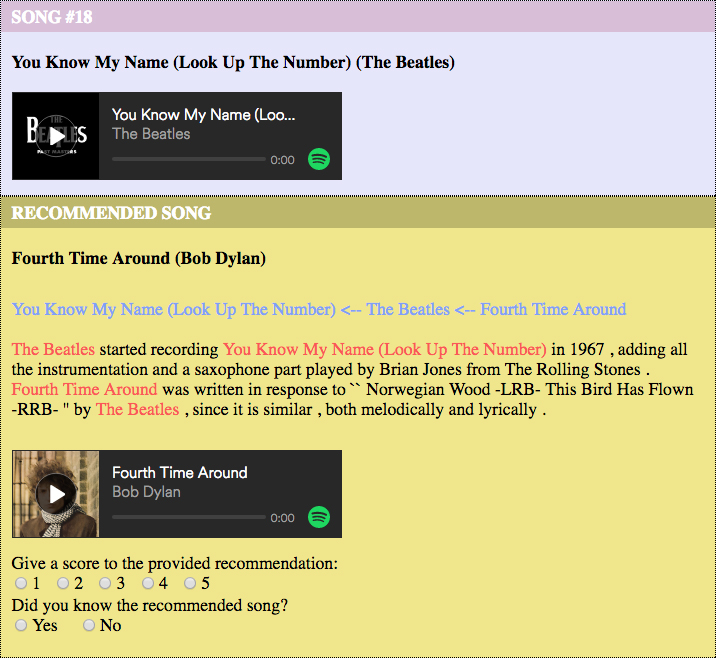
\includegraphics[width=0.8\textwidth]{ch04_kbconstruction_pics/recommender.jpg}}
\caption{User interface for the music recommendation experiment.}
\label{fig:kb:recommender}
\end{figure}


\section{Conclusion}\label{sec:kb:conclusions}

We have presented an NLP pipeline that extracts a Knowledge Base in the music domain taking raw text collections as input. It combines methods easily applicable to a general purpose application with domain-specific heuristics which are designed to exploit particularities of the domain.

The result of applying our approach over a dataset of stories about songs is a new Music Knowledge Base, which encodes semantic relations among musical entities. Our method relies on the syntactic structure (defined via dependency parsing) of sentences and the use and adaptation of music-specific heuristics for both Entity Linking and Relation Extraction. In addition, we include modules for semantic clustering and pattern scoring, aimed at the efficient removal of noisy relations. Our modular evaluation shows that our Relation Extraction module is able to capture a highly precise and compact set of weighted triples, and demonstrates the positive impact of the novel scoring metric we introduced. Moreover, we have shown that a high percentage of the knowledge encoded in our MKB is not present in other KBs, both general and domain-specific. Finally, regarding extrinsic evaluation, the experiment on recommendation interpretation confirms that explanations based on the extracted KB are positively regarded by the users.

%In the following chapter, we propose a method 

%We have identified several promising avenues for future work. For instance, we would like to extend our experiments to other music datasets of varied registers (e.g. social networks, magazines, encyclopedias), in order to fully understand the core differences between this domain and standard language. This should give an approximate idea of whether we need specific tools in certain specific NLP tasks. For instance, it seems reasonable to envision a music Entity Linking tool that is able to cope better with certain particularities of the domain.
%In addition, the development of new methodologies in Music Information Retrieval that exploit MKBs is still an open area of research.

\cleartorecto%!TEX root = ../thesis_a4.tex

\chapter{Applications in Musicology}
\label{sec:musicology}

\section{Introduction}
\label{sec:musicology:introduction}

A vast amount of musical knowledge has been gathered for centuries by musicologists and music enthusiasts. Most of this knowledge is implicitly expressed in artist biographies, reviews, facsimile editions, etc. %Music Digital Libraries make this information available and searchable. 
%In addition, with the democratisation of Internet access, large amounts of music information generated by users is stored in online sources. 
This context results in the existence of large repositories of unstructured knowledge, which have great potential for musicological studies.
%Keyword-based search is generally provided either in the context of a Digital Library or a Web browser. However, implicit knowledge present in text is not fully understood by machines, so complex queries cannot be answered. 
For instance, aggregating musical and musicological information after processing large collections of naturally occurring text can provide search engines with much richer and fine-grained information about musicians, their life and work, and even their relation with other musical entities.

In this chapter we propose to explore two use cases where we reconcile, on one hand, intelligent text processing techniques, and on the other, musical knowledge acquired both from structured and unstructured resources. In the first use case, we create a culture-specific knowledge base, in particular, a knowledge base of flamenco music. The methodology applied to its creation combines content aggregation from different data sources and knowledge extraction. Then, a methodology for the creation of a knowledge graph from a set of unstructured text documents using entity linking is proposed and tested for computing artist relevance ranking. Evaluation shows a high level of agreement between a flamenco expert and our system.
In the second use case, we provide a diachronic study of music criticism via a quantitative analysis of the polarity associated to music album reviews gathered from \texttt{Amazon}\footnote{\url{http://www.amazon.com}}. Our analysis hints at a potential correlation between key cultural and geopolitical events and the language and evolving sentiments found in music reviews. In addition, trends observed in the data reveals to be useful to study the evolution of music genres.

%In this chapter we address the challenge of making sense of large amounts of unstructured texts in the context of musicological studies from two different perspectives. 
%(1) we propose a methodology for the creation of a culture-specific knowledge base; in particular, a knowledge base of flamenco music. The proposed methodology combines content aggregation from different data sources and a knowledge extraction process. Then, a methodology for the creation of a Knowledge Graph is proposed and tested for computing artist relevance ranking. Evaluation shows a high level of agreement between a flamenco expert and our system. %First, an important amount of information is gathered from different data sources, which are subsequently combined by applying pair-wise entity resolution. Next, new knowledge is extracted from unstructured harvested texts and employed to populate the knowledge base. For this purpose, an entity linking system has been expressly developed. 
%(2) 
%We present an analysis of the evolution of Music Digital Libraries from a technological perspective. In addition, a methodology to exploit implicit knowledge present in this kind of libraries is proposed and applied over a set of artist biographies gathered from the New Grove Dictionary. 
%(2) we provide a diachronic study of music criticism via a quantitative analysis of the polarity associated to music album reviews gathered from Amazon. Our analysis hints at a potential correlation between key cultural and geopolitical events and the language and evolving sentiments found in music reviews. In addition, trends observed in the data reveals to be useful to study the evolution of music genres.

The rest of the chapter is organized as follows. First, in Section~\ref{sec:musicology:flamenco-kb}, we describe the process of creation of a culture-specific knowledge base. We begin introducing the problem and the context of application. Then, we describe the obtained knowledge base and the processes of knowledge curation and extraction applied. Finally, we employ the knowledge base to compute artist relevance ranking and present some insights that can be drawn from computing statistics over the dataset. In Section~\ref{sec:musicology:evolution}, we describe how sentiment associated with music reviews changes over time. We start by describing the dataset of music reviews used and the process of aspect-based sentiment analysis applied. Then, two experiments are performed, one aggregating sentiment scores by review publication year, and other by album publication year. Finally, we conclude the chapter with a discussion about our findings (Section~\ref{sec:musicology:conclusions}). 


\section{Building culture-specific knowledge bases: the flamenco case}
\label{sec:musicology:flamenco-kb}

%Music context information is now playing a key role in MIR research. Multimodal approaches, semantic approaches, and text-IR approaches have shown important achievements in typical MIR problems, such as music recommendation and discovery, genre classification, or music similarity \citep{Schedl2014}. Therefore, collecting and storing music context information may be extremely useful for the MIR research community. 

Although some existing repositories of music information are quite complete and accurate, there is still a vast amount of music information out there, which is generally scattered across different sources on the Web. Hence, harvesting and combining that information is a crucial step in the creation of practical and meaningful music knowledge bases. In addition, the creation of culture-specific knowledge bases may be highly valuable for research and dissemination purposes, and can be particularly impactful in non-western traditions \citep{Serra2014compmusic}. 
%However, to the best of our knowledege, not many initiatives have been focused on this direction.

In this section, we propose a methodology for the creation of a culture-specific knowledge base; in particular, a knowledge base of flamenco music. The proposed methodology combines content curation and knowledge extraction processes. First, a large amount of information is gathered from different data sources, which are subsequently combined by applying pair-wise entity resolution. Next, new knowledge is extracted from unstructured texts and employed to populate the knowledge base. To this end, an \textit{ad hoc} entity linking system has been developed. Finally, the content of the knowledge base is used to compute artist relevance and results are evaluated according to flamenco experts criteria. %The content of the knowledge base is freely available and downloadable as data dumps in RDF and JSON formats.

%The remainder of the section is organized as follows. In Section~\ref{sec:musicology:flamenco}, an introduction to flamenco music is presented. In Section~\ref{sec:musicology:related_work}  some relevant prior work is briefly surveyed. Section~\ref{sec:musicology:flabase} describes the structure of the knowledge base. Next, in Section~\ref{sec:musicology:kb_curation} the process of content curation is explained. Section~\ref{sec:musicology:kb_extraction} shows the methodology applied for knowledge extraction. In Section~\ref{sec:musicology:statistics} artist relevance is computed and some statistics about the content are laid out. Finally, Section~\ref{sec:musicology:conclusion} concludes the paper and points out for future lines of work.

\subsection{Flamenco music}
\label{sec:musicology:flamenco}

Several musical traditions contributed to the genesis of flamenco music as we know it today. Among them, the influences of the Jews, Arabs, and Spanish folk music are recognizable, but indubitably  the imprint of Andalusian Gypsies' culture is deeply ingrained in flamenco music. 
Flamenco occurs in a wide range of settings, including festive \textit{juergas} (private parties), \textit{tablaos} (flamenco venues), concerts, and big productions in theaters. In all these settings we find the main components of flamenco music: \textit{cante} or singing, \textit{toque} or guitar playing, and \textit{baile} or dance. According to \cite{gamboa-05}, flamenco music grew out of the singing tradition, as a melting process of all the traditions mentioned above, and therefore the role of the singer soon became dominant and fundamental. \textit{Toque}  is subordinated to \textit{cante}, especially in more traditional settings, whereas \textit{baile} enjoys more independence from voice. 

In the flamenco jargon styles are called \textit{palos}. Criteria adopted to define flamenco \textit{palos} are rhythmic patterns, chord progressions, lyrics and its poetic structure, and geographical origin. In flamenco geographical variation is important to classify \textit{cantes} as often they are associated to a particular region where they were originated or where they are performed with gusto. 
Rhythm or \textit{comp\'as} is a unique feature of flamenco.
Rhythmic patterns based on 12-beat cycles are mainly used. Those patterns can be classed as follows: binary patterns, such as \textit{tangos} or \textit{tientos}; ternary patterns, which are the most common ones, such as \textit{fandangos} or \textit{buler\'ias}; mixed patterns, where ternary and binary patterns alternate, such as \textit{guajira}; free-form, where there is no a clear underlying rhythm, such as \textit{ton\'as}.
For further information on fundamental aspects of flamenco music, see the book of Fern\'andez~\citep{fer-04}. For a comprehensive study of styles, musical forms and history of flamenco the reader is referred to the books of Blas Vega and R\'ios Ruiz~\citep{bvrr-88}, Navarro and Ropero~\citep{nr-95}, and Gamboa~\citep{gamboa-05} and the references therein.


\subsection{FlaBase}
\label{sec:musicology:flabase}

FlaBase (Flamenco Knowledge Base) is the acronym of a new knowledge base of flamenco music. Its ultimate aim is to gather all available online editorial, biographical and musicological information related to flamenco music. Its content is the result of the curation and extraction processes explained in Sections \ref{sec:musicology:kb_curation} and \ref{sec:musicology:kb_extraction}. %FlaBase is stored in RDF and JSON formats, and it is freely available for download\footnote{\url{http://mtg.upf.edu/download/datasets/flabase}}. Its RDF version follows the Linked Open Data principles, and it might be queried by setting up a SPARQL endpoint. A JSON version is also available, thus facilitating the use of the content by all the community of researchers and developers. 
FlaBase contains information about 1,174 artists, 76 \textit{palos} (flamenco genres), 2,913 albums, 14,078 tracks, and 771 Andalusian locations.

%Every entity in FlaBase is viewed as a resource, and every resource is classified by the FlaBase ontology.To define the properties of different classes of resources an initial ontology have been defined. In what follows, the ontology schema is shown and some statistics of the content available in Flabase are summarized.

\subsubsection{Ontology definition}
\label{sec:musicology:ontology}

The FlaBase data structure is defined following an ontology schema. One of the advantages of using an ontology is that it can be easily modified. Thus, our design is a first building block that can be enhanced and redefined in the future. The initial ontology is structured around five main classes: MusicArtist, Album, Track, Palo and Place, and three domain specific classes: \textit{cantaor} (flamenco singer), guitarist (flamenco guitar player), and \textit{bailaor} (flamenco dancer). These three classes were defined because they are the most frequent types of artists in the data. Other instrument players may be instantiated directly from the MusicArtist class. 
%A diagram with the main classes and some properties of the ontology is shown in Figure~\ref{fig:musicology:ontology}.
%We are aware of other music standard schemas such as the Music Ontology \footnote{\url{http://musicontology.com/}}, however, we opted to define our own ontology in order to let the schema as simple as possible. By the way, class and property equivalence has been defined through the OWL\footnote{\url{http://www.w3.org/TR/owl2-overview/}} properties owl:equivalentClass and owl: equivalentProperty between our classes and properties and those from the Music Ontology (e.g. MusicArtist, Track, Genre).
We have tried to reuse as much vocabulary as we could. We re-utilized most of the classes and some properties from the Music Ontology\footnote{\url{http://musicontology.com}}, a standard model for publishing music-related data. We selected the classes according to the ones used by the LinkedBrainz project\footnote{\url{https://wiki.musicbrainz.org/LinkedBrainz}}, which maps concepts from MusicBrainz to Music Ontology.

\iffalse
\begin{figure}
	\centering
	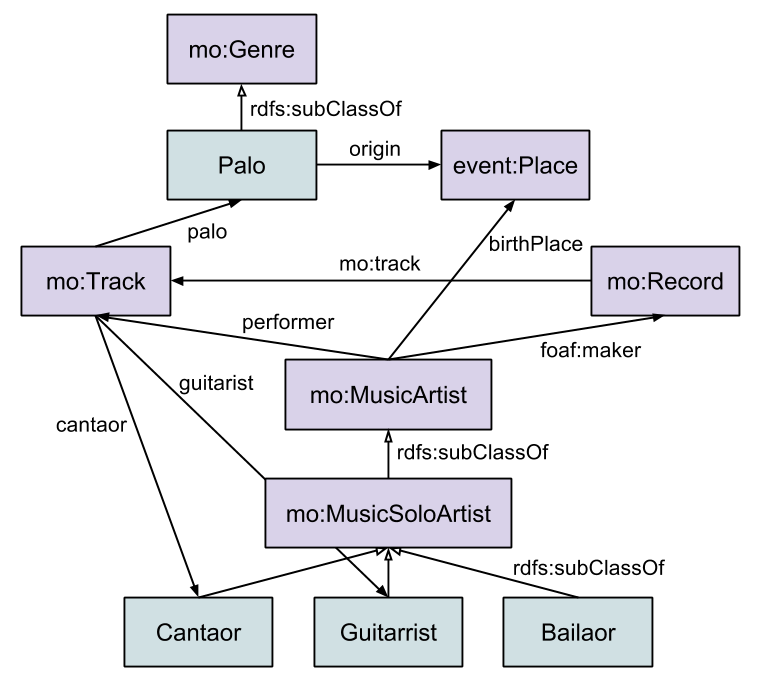
\includegraphics[width=0.40\textwidth]{ch05_musicology_pics/flabase_ontology2.png}
	\caption{Ontology schema \label{fig:musicology:ontology}}
\end{figure}
\fi


\subsection{Content curation}
\label{sec:musicology:kb_curation}

The first step towards building a domain-specific knowledge base is to gather all possible content from available data sources. This implies at least two problems, namely, the selection of sources, and the matching between entities from different sources (entity resolution). In what follows we enumerate the involved data sources and describe the methodology applied for entity resolution.

\subsubsection{Data acquisition}
\label{sec:musicology:datasoruces}

Our aim is to gather an important amount of information about musical entities, including textual descriptions and available metadata. A schema of the selected data sources is shown in Figure~\ref{fig:musicology:datasources}. We started by looking at Wikipedia.%, the free and multilingual Internet encyclopedia. It is the Internet's largest and most popular general reference work. 
Each Wikipedia article may have a set of associated categories. Categories are intended to group together pages on similar subjects and are structured in a taxonomical way. To find Wikipedia articles related to flamenco music, we first looked for flamenco categories. The taxonomy of categories can be explored by querying DBpedia. %, a knowledge base with structured content extracted from Wikipedia. 
In particular, we employed the SPARQL endpoint of the Spanish DBpedia\footnote{\url{http://es.dbpedia.org}}. We queried for categories related to the flamenco category in the taxonomy. At the end, we obtained 17 different categories (e.g., \textit{cantaores de flamenco, guitarristas de flamenco}).

\begin{figure}
	\centering
	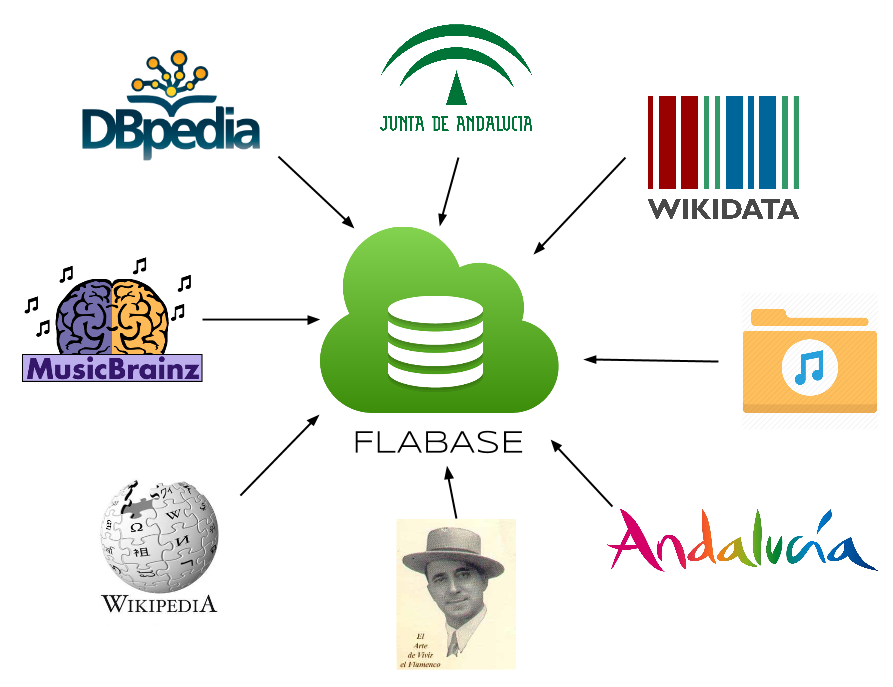
\includegraphics[width=0.45\textwidth]{ch05_musicology_pics/datasources.png}
	\caption{Selected data sources \label{fig:musicology:datasources}}
\end{figure}

%DBpedia resources are related to categories through the property dcterms:subject. Thus, b
By querying again DBpedia, we gathered all DBpedia resources related to one of these categories. We obtained a total number of 438 resources in Spanish, of which 281 were also in English. Each DBpedia resource is associated with a Wikipedia article. Text and HTML code were then extracted from Wikipedia articles in English and Spanish by using the WikiMedia API. 
%From DBpedia, we also gathered some biographical structured information of each resource, when it was available. 
Next, we classified the extracted articles according to our ontology (Section~\ref{sec:musicology:ontology}). For this purpose, we exploited classification information provided by DBpedia (DBpedia types and Wikipedia categories). At the end, from all gathered resources, we only kept those related to artists and \textit{palos}, totalling  291 artists and 56 \textit{palos}.

As the amount of information present in Wikipedia related to flamenco music is somewhat scarce, we decided to expand our knowledge base with information from two different websites. First, \textit{Andalucia.org}, the touristic web from the Andalusia Government\footnote{\url{http://andalucia.org}}. It contains 422 artist biographies in English and Spanish, and the description of 76 \textit{palos} also in both languages. Second, a website called \textit{El arte de vivir el flamenco}\footnote{\url{http://www.elartedevivirelflamenco.com/}}, which includes 749 artist biographies among \textit{cantaores}, \textit{bailaores} and guitarists. Both webs were crawled and their content stored in our knowledge base. %As it is explained in Section~\ref{sec:musicology:entity_resolution}, artists from the three datasources were mapped, obtaining a final set of 1,176 different artists.

%MusicBrainz is one of the biggest and more reliable open music databases, which provides an unambiguous form of music identification. Therefore, we turned to it 
We used MusicBrainz to fill our knowledge base with information about flamenco album releases and recordings. Artists present in FlaBase were intended to be mapped with MusicBrainz artists. For every match, all content related to releases and recordings was gathered. After doing so, we obtained a total number of 814 releases and 9,942 recordings. 
%AcousticBrainz\footnote{\url{http://acousticbrainz.org}} is a project that aims to crowd source acoustic information for all music tracks identified in MusicBrainz. We queried the AcousticBrainz API for the acoustic descriptors of MusicBrainz recordings. We found acoustic information of 620 of the stored recordings.%, and kept it in our knowledge base.

The information gathered from MusicBrainz is a little part of the actual flamenco discography. Therefore, to complement it we used a flamenco recordings database gathered by Rafael Infante and available at CICA website\footnote{\url{http://flun.cica.es/index.php/grabaciones}} (Computing and Scientific Center of Andalusia). This database has information about releases from the early time of recordings until present time, counting 2,099 releases and 4,136 songs. For every song entry, a \textit{cantaor} name is provided, and most of the times also guitarist and \textit{palo}, which is an important piece of information to define flamenco recordings.

Finally, we supplied our knowledge base with information related to Andalusian towns and provinces. We gathered this information from the official database SIMA\footnote{\url{http://www.juntadeandalucia.es/institutodeestadisticaycartografia/sima}} (Multi-territorial System of Information of Andalusia).%, of the Official Institute of Statistics and Cartography of Andalusia. 


\subsubsection{Entity resolution}
\label{sec:musicology:entity_resolution}

Entity resolution is the problem of extracting, matching and resolving entity mentions in structured and unstructured data \citep{Getoor2012}. There are several approaches to tackle the entity resolution problem. For the scope of this research, we selected a pair-wise classification approach based on string similarity between entity labels.

The first issue after gathering the data is to decide whether two entities from different sources are referring to the same one. Therefore, given two sets of entities $A$ and $B$, the objective is to define an injective and non-surjective mapping function $f$ between $A$ and $B$ that decides whether an entity $a \in A$ is the same as an entity $b \in B$. To do that, a string similarity metric $sim(a,b)$ based on the Ratcliff-Obershelp algorithm \citep{Ratcliff1988} has been defined. It measures the similarity between two entity labels and outputs a value between 0 and 1. We consider that $a$ and $b$ are the same entity if their similarity is bigger than a parameter $\theta$. If there are two entities $b, c \in B$ that satisfy that $sim(a,b) \geq \theta$ and $sim(a,c) \geq \theta$, we consider only the mapping with the highest score. To determine the value of $\theta$, we tested the method with several $\theta$ values over an annotated dataset of entity pairs. To create this dataset, the 291 artists gathered from Wikipedia were manually mapped to the 422 artists gathered from Andalucia.org, obtaining a total amount of 120 pair matches. As it is shown in Figure~\ref{fig:musicology:fmeasure} the best F-measure (0,97) was obtained with $\theta=0.9$. Finally, we applied the described method with $\theta=0.9$ to all gathered entities from the three data sources. Thanks to the entity resolution process, we reduced the initial set of 1,462 artists and 132 \textit{palos} to a set of 1,174 artists and 76 \textit{palos}.

\begin{figure}
	\centering
	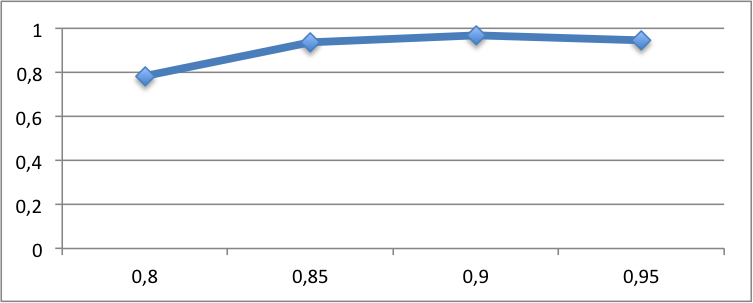
\includegraphics[width=0.40\textwidth]{ch05_musicology_pics/similarity_f.png}
	\caption{F-measure for different values of $\theta$ \label{fig:musicology:fmeasure}}
\end{figure}

Once we had our artist entities resolved, we began to gather their related discographic information. First, we tried to find out the MusicBrainz ID of the gathered artists. Depending on the information about the entity, two different process were applied. First, every Wikipedia page has a correspondent entity defined in Wikidata\footnote{\url{https://www.wikidata.org}}. Wikidata is a free linked database which acts as a structured data storage of Wikipedia. There are several properties in Wikidata that may link Wikidata items with MusicBrainz items. %Thus, the equivalent Wikidata resource of a Wikipedia artist page may have a link to its corresponding MusicBrainz artist ID. 
We looked for these relations and mapped all possible entities. For those artists without a direct link to MusicBrainz, we queried the MusicBrainz API by using the artists names, and then applied our entity resolution method to the obtained results.

Finally, to integrate the discography database of CICA into our knowledge base, we applied the entity resolution method to the fields \textit{cantaor}, guitarist and \textit{palo} of each recording entry in the database. From the set of 202 \textit{cantaores} and 157 guitarists names present in the recording entries of the database, a total number of 78 \textit{cantaores} and 44 guitarists were mapped to our knowledge base. The number of mapped artists was low due to differences between the way of labeling an artist. An artist name may be written using one or two surnames, or using a nickname. In the case of \textit{palos}, there were 162 different \textit{palos} in the database, 54 of which were mapped with the 76 of our knowledge base. These 54 \textit{palos} correspond to an 80\% of \textit{palo} assignments present in the recording entries.


\subsection{Knowledge extraction}
\label{sec:musicology:kb_extraction}

While the resulting knowlege base does already encode relevant culture and music-specific information, a notable portion of the data collected during the knowledge base creation process currently remains unexploited due to its unstructured nature. In fact, the huge epistemic potential of free text in this version of the knowledge base has not still been harnessed. Consequently, to enhance the amount of structured data in FlaBase, a process of knowledge extraction has been carried out. This implicit knowledge may vary from biographical data, such as place and date of birth, to more complex semantic relations involving different entities. Three tasks play a key role in the process of knowledge extraction from non-structured text: named entity recognition (NER), entity linking (EL), and relation extraction \citep{Usbeck2014}. In this section, we focus on the two first tasks. In what follows, our \textit{ad hoc} system for entity recognition and disambiguation is described and evaluated. Lastly, an information extraction process is applied to populate the knowledge base.

\subsubsection{Named entity recognition and disambiguation}\label{sec:musicology:entity_linking}

In order to extract knowledge from a text, the first step is to semantically annotate it identifying all entity mentions. %Named entity recognition is a task that seeks and classify words in text into pre-defined categories (e.g., person, organization, or place). Named entity disambiguation, also called entity linking, aims to determine what is actually a named entity present in a text. It generally does so by identifying it in a knowledge base of reference. 
Entity linking can be addressed directly from the text, or applied to the output of a NER system. We propose a method that employs a combination of both approaches, depending on the category of the entity. For NER, we used the Stanford NER system \citep{Finkel2005}, implemented in the library Stanford Core NLP\footnote{\url{http://nlp.stanford.edu/software/corenlp.shtml}} and trained on Spanish texts. For EL we applied two different approaches. First, we looked for exact string matches between FlaBase entity labels and word n-grams extracted from the text. Second, we searched for exact string matches between FlaBase entity labels and named entities identified of the NER system. We tried several combinations of both approaches until we obtained the most satisfactory one.

%We selected all biography texts in Spanish from artists present in our knowledge base. 
For the scope of this research, we focused on Spanish texts, as flamenco texts are mostly written in Spanish. Although there are many entity linking tools available, state-of-the-art systems are well-tuned for English texts, but may not perform as well in languages other than English, and even less with music related texts (see Section~\ref{sec:linking:el}). In addition, we wanted to have a system that uses our own knowledge base. Therefore, we developed our own system, which is able to detect and disambiguate three categories of entities: person, \textit{palo} and location. Three different approaches were defined by combining NER and EL in different ways. First, directly applying EL to text. Second, disambiguating location and person entities from the NER output, and \textit{palo} directly from text. Third, only disambiguating location entities from the NER output, and location and \textit{palo} directly from text.

To determine which approach performs better, three artist biographies coming from three different data sources were manually annotated, having a total number of 49 annotated entities. We followed an evaluation methodology similar to the one used in KBP2014 Entity Linking Task\footnote{\url{http://nlp.cs.rpi.edu/kbp/2014/}}. Results on the different approaches are shown in Table~\ref{tbl:musicology:res1}. We observe that applying NER to entities of the person category before EL worsens performance significantly, as recall suddenly decreases by half. After manually analyzing false negatives, we observed that this is caused because many artist names have definite articles between name and surname (e.g., \textit{de, del}), and this is not recognized by the NER system. In addition, many artists have a nickname that is not interpreted as a person entity by the NER system. The best approach is the third (EL + NER to LOC), which is slightly better than the first (only EL) in terms of precision. This is due to the fact that many artists have a town name as a surname or as part of his nickname. Therefore, applying EL directly to text is misclassifying person entities as location entities. Thus, by adding a previous step of NER to location entities we have increased overall performance, as it can be seen on the F-measure values.

\begin{table}
	\centering
%\begin{adjustbox}{max width=8cm}
	  \begin{tabular}{ | l | c | c | c | }
    \hline
    Approach & Precision & Recall & F-measure \\ \hline
    \hline
    1) EL & 0.829 & \textbf{0.694} & 0.756 \\ 
    2) EL + NER to PERS \& LOC & 0.739 & 0.347 & 0.472 \\
    3) EL + NER to LOC & \textbf{0.892} & 0.674 & \textbf{0.767} \\
    \hline
  \end{tabular}
%  \end{adjustbox}
	\caption{Precision, Recall and F-measure of NER+EL}
	
	\label{tbl:musicology:res1}
\end{table}

\subsubsection{Knowledge base population}
\label{sec:musicology:ie}

Biographical texts coming from different data sources have been stored in FlaBase. These texts are full of relevant information about FlaBase entities, but in an unstructured way. Thus, a process of information extraction is necessary to transform the unstructured information into structured knowledge. For the scope of this research, we focused on extracting two specific pieces of information: birth year and birth place, as they can be relevant for anthropological studies. We observed that this information is often in the first sentences of the artist biographies, and always near the word \textit{naci\'{o}} (Spanish translation of ``was born"). Therefore, to extract this information, we looked for this word in the first 250 characters of every biographical text. If it is found, we apply our entity linking method to this piece of text. If a location entity is found near the word "naci\'{o}", we assume that this entity is the place of birth of the biography subject. In addition, by using regular expressions, we look for the presence of a year expression in the neighborhood. If it is found, we assume it as the year of birth. If more than one year is found, we select the one with the smaller value. 

To evaluate our approach, we tested the extraction of birth places in all texts coming from the web Andalucia.org (442 artists). %We chose this subset because Andalucia.org also provides specific information about artist origin that had been previously crawled and stored in FlaBase. However, we observed that in many occasions the artist origin provided by the data source was wrong. Therefore, we decided to 
We manually annotated the province of provenance of these 442 artists for building ground truth data. After the application of the extraction process on the annotated test set, we obtained a precision value of 0,922 and a recall of 0,648. Therefore, we may argue that our method is extracting biographic information with high precision and quite reasonable recall. 
%In addition, the information extracted by our system is indeed more accurate than the actual information provided by the data source. 
We finally applied the extraction process to all artist entities with biographical texts coming from any of the two flamenco crawled websites. Thus, %from a total number of 1,123 artists coming from these data sources (95\% of the artists in the knowledge base), 
743 birth places and 879 birth years were extracted. 

\subsection{Looking at the data}
\label{sec:musicology:data-analysis}

\subsubsection{Artist relevance}
\label{sec:musicology:relevance}

We assume that an entity mention inside an artist biography signals a semantic relation between the entity that constitutes the main theme of the biography (subject entity) and the mentioned entity. Based on this assumption, we build a semantic graph by applying the following steps. First, each artist of the knowledge base is added to the graph as a node. Second, entity linking is applied to artist's biographical texts. For every linked entity identified in the biography, a new node is created in the graph (only if it was not previously created). Next, an edge is added, connecting the subject entity with the linked entity found in its biography. This way, a directed graph connecting the entities of FlaBase is finally obtained. Entities identified in a text can be seen as hyperlinks. Thus, algorithms to measure the relevance of nodes in a network of hyperlinks can be applied to our semantic graph \citep{Bellomi2005}. In order to measure artist relevance, we applied PageRank \citep{Brin1998} and HITS \citep{Kleinberg1999} algorithms to the obtained graph. 
%PageRank outputs a measure of relevance for each node, and HITS gives two different results: \textit{authority} and \textit{hubness}. We only take into consideration \textit{authority} from HITS algorithm, because it is proven to be the most effective of both values as a relevancy metric \citep{Bellomi2005}.

Using this approach, we built an ordered list with the top-10 entities of the different artist categories (\textit{cantaor}, guitarist and \textit{bailaor}) for the two algorithms. For evaluation purposes, we asked a reputed flamenco expert to build a list of top-10 artists for each category according to his knowledge and the available bibliography. The concept of artist relevance is somehow subjective and there is no unified or consensual criteria for flamenco experts about who the most relevant artists are. Despite that, there is a high level of agreement among them on certain artists that should be on such a hypothetical list. Thus, the expert provided us with this list of hypothetical top-10 artists by category and we considered it as ground truth. We define precision as the number of identified artists in the resulting list that are also present in the ground truth list divided by the length of the list. We evaluated the output of the two algorithms by calculating precision over the entire list (top-10), and over the first five elements (top-5) (see Table~\ref{tbl:musicology:experts_results}). We can observe that Page\-Rank results (see Table~\ref{tbl:musicology:pagerank}) show the greatest agreement with the flamenco expert. 
High values of precision, especially for the top-5 list, indicates that the content gathered in FlaBase is highly complete and accurate (see Table~\ref{tbl:musicology:experts_results}), and the proposed methodology adequate to compute relevance of artists. 

\inputencoding{latin1}
\begin{table}[!ht]
    \centering
%\begin{adjustbox}{max width=8cm}
    \begin{tabular}{|c|c|c|}
    \hline
    \textit{Cantaor} & Guitarist & \textit{Bailaor} \\
    \hline
Antonio Mairena & Paco de Luc\'{i}a & Antonio Ruiz Soler \\
Manolo Caracol & Ram\'{o}n Montoya & Rosario \\
La Ni\~{n}a de los Peines & Ni\~{n}o Ricardo & Antonio Gades \\
Antonio Chac\'{o}n & Manolo Sanl\'{u}car & Mario Maya \\
Camar\'{o}n de la Isla & Sabicas & Carmen Amaya \\
%Manuel Torre & Tomatito & Pilar López \\
%José Mercé & Vicente Amigo & La Argentinita \\
%Enrique Morente & Gerardo Núñez & Lola Flores \\
%Pepe Marchena & Paco Cepero & Pastora Imperio \\
%Manuel Vallejo & Pepe Habichuela & José Antonio \\
    \hline
    \end{tabular}
%   \end{adjustbox}
    \caption{PageRank Top-5 artists by category}    
    \label{tbl:musicology:pagerank}
\end{table}
\inputencoding{utf8}

%Among the different categories, the list of \textit{cantaores} exhibit the best agreement with the ground truth. This is probably due to the fact that there is more information about this particular category in FlaBase (47\% of \textit{cantaores}, 29\% of guitarists, and 22\% of \textit{bailaores)}. 
%As it is shown in Figure~\ref{fig:musicology:graph-type}, the amount of cantaores is substantially higher than the other two categories.


\begin{table}[!ht]
    \centering
%\begin{adjustbox}{max width=8cm}
    \begin{tabular}{|c|c|c|}
    \hline
    & Top-5 & Top-10 \\
    \hline
    PageRank & 0.933 & 0.633 \\
    HITS Authority & 0.6 & 0.4 \\
    \hline
    \end{tabular}
%   \end{adjustbox}
    \caption{Precision values}    
    \label{tbl:musicology:experts_results}
\end{table}

\subsubsection{Statistics}
\label{sec:musicology:statistics}

For the sake of completeness, we computed the distribution of different items present in FlaBase. 
% after the processes of curation and extraction.  
Data shown in Figure~\ref{fig:musicology:graph-palo} was produced after the knowledge acquisition process, while data shown in Figures \ref{fig:musicology:graph-province} and \ref{fig:musicology:graph-decade} was obtained thanks to the knowledge extraction process. In Figure~\ref{fig:musicology:graph-palo} it is shown that the most representative \textit{palos} in flamenco music are represented in our knowledge base, with a higher predominance of fandangos. We can observe in Figure~\ref{fig:musicology:graph-province} that most flamenco artists are from the Andalusian provinces of Seville and Cadiz. 
Finally, in Figure~\ref{fig:musicology:graph-decade} we observe a higher number of artists in the data were born from the 30's to the 80's of the 20th century.

%\begin{figure}
%    \centering
%    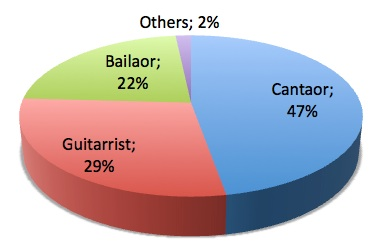
\includegraphics[width=6cm]{figs/Artists-by-type.jpg}
%    \caption{Artists by type 
%    \label{fig:musicology:graph-type}}
%\end{figure}

\begin{figure}[ht!]
    \centering
    \begin{subfigure}{.45\textwidth}
        \centering
        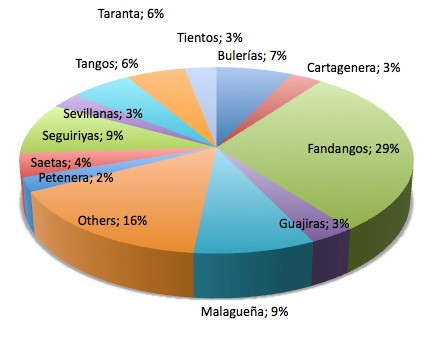
\includegraphics[width=.9\linewidth]{ch05_musicology_pics/Songs-by-palo.jpg}
    	\caption{Songs by \textit{palo}}
        \label{fig:musicology:graph-palo}
    \end{subfigure}
    \begin{subfigure}{.50\textwidth}
        \centering
        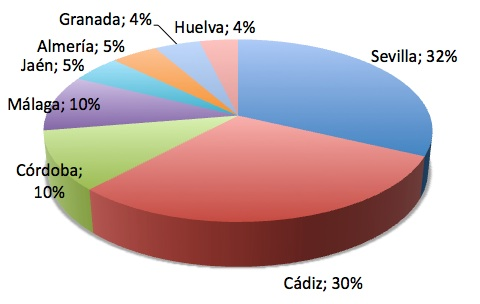
\includegraphics[width=.9\linewidth]{ch05_musicology_pics/Artists-by-province.jpg}
		\caption{Artists by province of birth}
		\label{fig:musicology:graph-province}
    \end{subfigure}
\end{figure}


\begin{figure}[!ht]
	\centering
	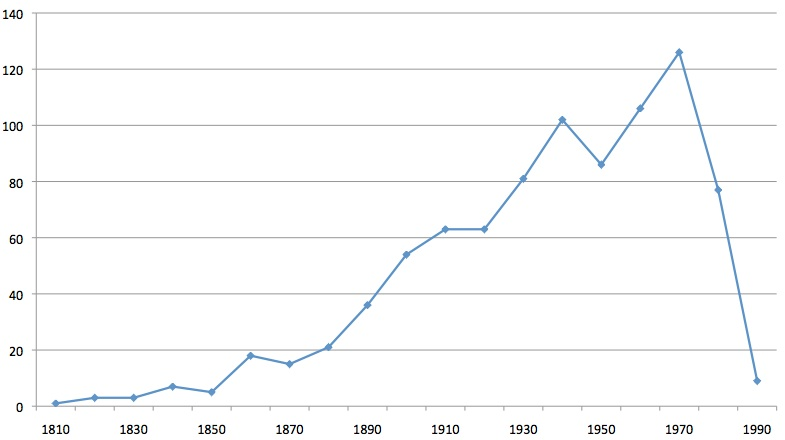
\includegraphics[width=8cm]{ch05_musicology_pics/Artists-by-decade-of-birth.jpg}
	\caption{Artists by decade of birth 
	\label{fig:musicology:graph-decade}}
\end{figure}


\section{Diachronic study of music criticism}
\label{sec:musicology:evolution}

In this Section, we put forward an integration procedure for enriching a large corpus of Amazon customer reviews \citep{McAuley2015a,McAuley2015}, with metadata obtained from MusicBrainz\footnote{\url{http://musicbrainz.org/}}. %AcousticBrainz (AB) is a database of music and audio descriptors, computed from audio recordings via state-of-the-art Music Information Retrieval algorithms \citep{Porter2015}.
In addition, we further extend the \textit{semantics} of the textual content with the application of an aspect-based sentiment analysis framework \citep{DongSOS13} which provides specific sentiment scores for different aspects present in the text, e.g. album cover, guitar, voice or lyrics.

This enriched dataset, henceforth referred to as Multimodal Album Reviews Dataset (MARD), includes affective features and music metadata. % such as album release date.
We benefit from this substantial amount of information at our disposal for performing a diachronic analysis of music criticism. Specifically, we combine the metadata retrieved for each review with their associated sentiment information, and generate visualizations to help us investigate any potential trends in diachronic music appreciation and criticism. Based on this evidence, and since music evokes emotions through mechanisms that are not unique to music \citep{Juslin2008}, we may go as far as using musical information as means for a better understanding of global affairs. Previous studies argue that national confidence may be expressed in any form of art, including music \citep{Moisi2010}, and in fact, there is strong evidence suggesting that our emotional reactions to music have important and far-reaching implications for our beliefs, goals and actions, as members of social and cultural groups \citep{Alcorta2008}. Our analysis hints at a potential correlation between the language used in music reviews and major geopolitical events or economic fluctuations. Finally, we argue that applying sentiment analysis to music corpora may be useful for diachronic musicological studies.


\subsection{Dataset}
\label{sec:musicology:mard}

The collected dataset contains texts and accompanying metadata originally obtained from a much larger dataset of Amazon customer reviews \citep{McAuley2015a,McAuley2015}. The original dataset provides millions of review texts together with additional information such as overall rating (between 0 to 5), date of publication, or creator id. Each review is associated to a product and, for each product, additional metadata is also provided, namely Amazon product id, list of similar products, price, sell rank and genre categories. From this initial dataset, we selected the subset of products categorized as \textit{CDs \& Vinyls}, which also fulfill the following criteria. First, considering that the Amazon taxonomy of music genres contains 27 labels in the first hierarchy level, and about 500 in total, we obtain a music-relevant subset and select 16 of the 27 which really define a music style and discard for instance region categories (e.g. World Music) and other categories non specifically related to a music style (e.g. Soundtrack, Miscellaneous, Special Interest), function-oriented categories (Karaoke, Holiday \& Wedding) or categories whose albums might also be found under other categories (e.g. Opera \& Classical Vocal, Broadway \& Vocalists). We compiled albums belonging only to one of the 16 selected categories, i.e. no multi-label. Note that the original dataset contains not only reviews about CDs and Vinyls, but also about music DVDs and VHSs. Since these are not strictly speaking music audio products, we filter out those products also classified as "Movies \& TV". Finally, since products classified as Classical and Pop are substantially more frequent in the original dataset, we compensate this unbalance by limiting the number of albums of any genre to 10,000. After this preprocessing, MARD amounts to a total of 65,566 albums and 263,525 customer reviews. A breakdown of the number of albums per genre is provided in Table~\ref{tbl:musicology:dataset}.

%This dataset is formed by texts and metadata coming from Amazon costumers reviews from the "CDs \& Vinyls" section. It is a subset of a large dataset of costumer reviews gathered in \cite{McAuley2015a,Mauch150081}. Review texts come with some extra information , i.e. overall rating, date of publication and creator id. Every review is related to a music album. For every album there is also some attached information, i.e. title, Amazon product id, list of similar products, price, sell rank and genre categories. From the initial dataset, we selected those products that fulfill the following criteria. The Amazon taxonomy of genres has 27 genres in the first hierarchy level, and more than 500 in total. From the 27 categories, we selected 16 define a music style, and not a region (e.g. Asian music) or another classification criteria (e.g. Soundtrack). We selected albums that are classified into only one of 16 selected categories. The original dataset has not only reviews about CDs and Vinyls, but also music DVDs and VHSs. Hence, to focus only on audio products, we filter out products that were also categorized as "Movies \& TV" or were ranked in the Video sales ranking. In the original dataset, there is a higher predominance of products classified as Classical and Pop. To compensate that, we limited the number of albums of these genres to 10,000 in the final dataset. After the filtering process we kept a total of 65,566 albums and 263,525 customer reviews, which comprises the core of our dataset. The amount of albums by genre is shown in Table~\ref{tbl:musicology:dataset}.

\begin{table}[h]
\scriptsize
\centering
\begin{tabular}{|l|r|r|r|}
\hline
\textbf{Genre} & \textbf{Amazon} & \textbf{MusicBrainz} \\%& \textbf{AcousticBrainz} \\
\hline
Alternative Rock & 2,674 & 1,696 \\%& 564 \\
Reggae & 509 & 260 \\%& 79 \\
Classical & 10,000 & 2,197 \\%& 587 \\
R\&B & 2,114 & 2,950 \\%& 982 \\
Country & 2,771 & 1,032 \\%& 424 \\
Jazz & 6,890 & 2,990 \\%& 863 \\
Metal & 1,785 & 1,294 \\%& 500 \\
Pop & 10,000 & 4,422 \\%& 1701 \\
New Age & 2,656 & 638 \\%& 155 \\
Dance \& Electronic & 5,106 & 899 \\%& 367 \\
Rap \& Hip-Hop & 1,679 & 768 \\%& 207 \\
Latin Music & 7,924 & 3,237 \\%& 425 \\
Rock & 7,315 & 4,100 \\%& 1482 \\
Gospel & 900 & 274 \\%& 33 \\
Blues & 1,158 & 448 \\%& 135 \\
Folk & 2,085 & 848 \\%& 179 \\
\hline
\textbf{Total} & 66,566 & 28,053 \\%& 8,683 \\
\hline
\end{tabular}
\caption{Number of albums by genre with information from the different sources in MARD}
\label{tbl:musicology:dataset}
\end{table}

Having performed genre filtering, we enrich MARD by extracting artist names and record labels from the Amazon product page. We pivot over this information to query the MusicBrainz search API to gather additional metadata such as release id, first release date, song titles and song ids. Mapping with MusicBrainz is performed using the same methodology described in Section~\ref{sec:musicology:entity_resolution}, following a pair-wise entity resolution approach based on string similarity with a threshold value of $\theta=0.85$. We successfully mapped 28,053 albums to MusicBrainz. %Then, we retrieved songs' audio descriptors from AB. From the 28,053 albums mapped to MusicBrainz, a total of 8,683 albums are further linked to their corresponding AB entry, which encompasses 65,786 songs. The final dataset is freely available for download\footnote{http://mtg.upf.edu/download/datasets/mard}.


%Note that this is the number of songs present in AB at the time of the dataset creation, however, AB is continuously growing and more albums from the total mapped to MB might be also found in the future in AB. 

%A summary of the properties of our dataset and the interplay of the three resources is shown in Figure \ref{fig:musicology:dataset}, using the album ``The Adventures of Rick Slick'' (Rick Slick) as an example.

%\begin{figure}[!h]
%  \centering
%	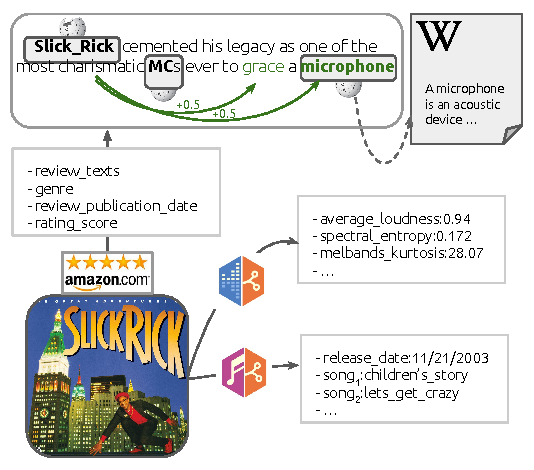
\includegraphics[width=8cm,height=7.25cm]{figs/dataset}
%  \caption{Summary of enrichment for every album review in our dataset, containing ontological (MB) and acoustic (AB) information as well as textual semantics.}
%  \label{fig:musicology:dataset}
%\end{figure}

%Once this genre-wise filtering was performed, we enrich the original ADR with artist name and record label. retrieved some extra information from Amazon that was not included in the original dataset, i.e. artist name and record label. Using the artist name and the album title we queried the MusicBrainz search API to try to gather more metadata about the albums, i.e. release group MBID (MusicBrainz ID), first release date, song titles and song MBID. For the mapping with MusicBrainz we followed a methodology similar to the one described in \cite{Flabase}. From the filtered set of albums, we obtained a mapping with MusicBrainz of 28,053 albums. Having the  MBIDs of the album songs, we can retrieve their audio descriptors present in AcousticBrainz. AcousticBrainz is a database of music descriptors computed from audio recordings using a number of state-of-the-art Music Information Retrieval algorithms. From the albums mapped to MusicBrainz, we found 8,683 albums for which their song descriptors were stored in AcousticBrainz. Audio descriptors of a total number of 65,786 songs were retrieved from AcousticBrainz.


\subsection{Sentiment analysis}
\label{sec:musicology:sentiment}

\begin{figure}
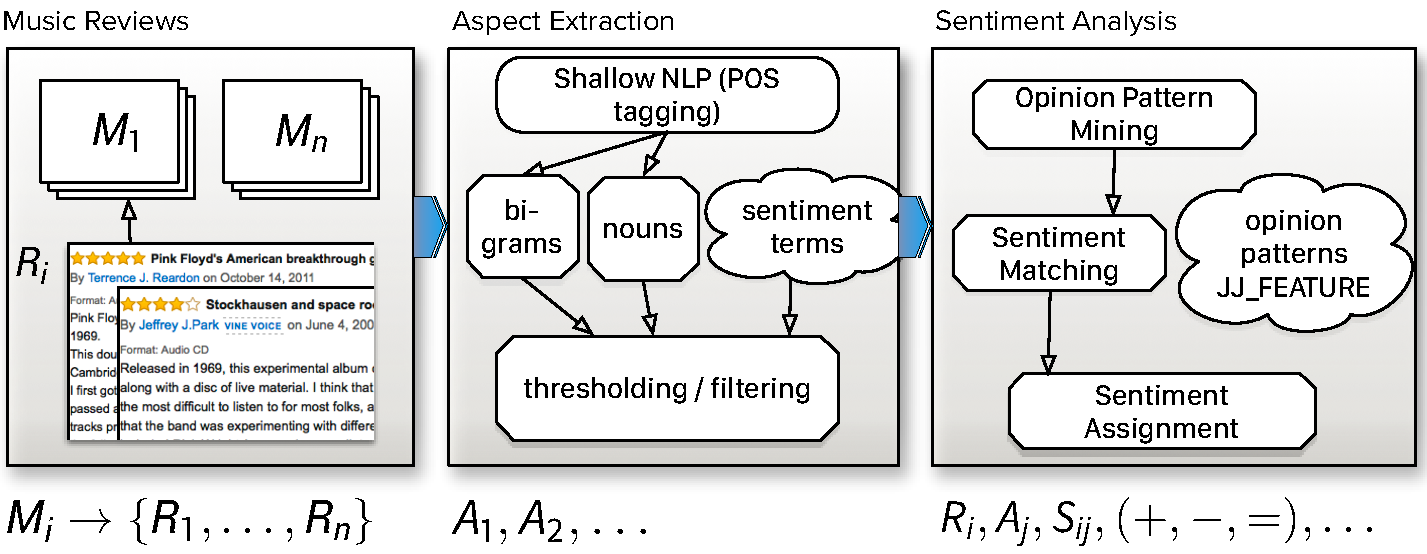
\includegraphics[width=\columnwidth]{ch05_musicology_pics/omf}
\caption{Overview of the opinion mining and sentiment analysis framework.}
\label{fig:musicology:OMF}
\end{figure}

Following the work of \cite{DongSOS13,DongOS14} we use a combination of shallow NLP, opinion mining, and sentiment analysis to extract opinionated features from reviews. For reviews $R_{i}$ of each album, we mine bi-grams and single-noun aspects (or review features), see \cite{Hu2004}; e.g. bi-grams which conform to a noun followed by a noun (e.g. \emph{chorus arrangement}) or an adjective followed by a noun (e.g. \emph{original sound}) are considered, excluding bi-grams whose adjective is a sentiment word (e.g. \emph{excellent}, \emph{terrible}). Separately, single-noun aspects are validated by eliminating nouns that are rarely associated with sentiment words in reviews, since such nouns are unlikely to refer to item aspects. We refer to each of these extracted aspects $A_{j}$ as review aspects.

For a review aspect $A_{j}$ we determine if there are any sentiment words in the sentence containing $A_{j}$. If not, $A_{j}$ is marked neutral, otherwise we identify the sentiment word $w_{min}$ with the minimum word-distance to $A_j$. Next we determine the part-of-speach tags for $w_{min}$, $A_i$ and any words that occur between $w_{min}$ and $A_i$. 
%This POS sequence is an opinion pattern. We compute the frequency of all opinion patterns in all reviews; a pattern is valid if it occurs more than average. For valid patterns, we assign sentiment score between -1 and 1 to $A_j$ based on the sentiment of $w_{min}$ and subject to whether the corresponding sentence contains any negation terms within $4$ words of $w_{min}$. 
We assign a sentiment score between -1 and 1 to $A_j$ based on the sentiment of $w_{min}$, subject to whether the corresponding sentence contains any negation terms within $4$ words of $w_{min}$. If there are no negation terms, then the sentiment assigned to $A_j$ is that of the sentiment word in the sentiment lexicon; otherwise this sentiment is reversed. Our sentiment lexicon is derived from SentiWordNet \citep{esuli2006sentiwordnet} and is not specifically tuned for music reviews.
%If an opinion pattern is not valid then we assign a neutral sentiment to each of its occurrences within the review set; see \cite{Moghaddam2010} for a more detailed description. 
An overview of the process is shown in Figure~\ref{fig:musicology:OMF}. The end result of sentiment analysis is that we determine a sentiment label $S_{ij}$ for each aspect $A_j$ in review $R_i$. A sample annotated review is shown in Figure~\ref{fig:musicology:annotatedreview}.
Finally, the sentiment score of a review $R_i$ is calculated as the average of the sentiment score of every aspect $A_j$ in $R_i$.

\begin{figure}[h]
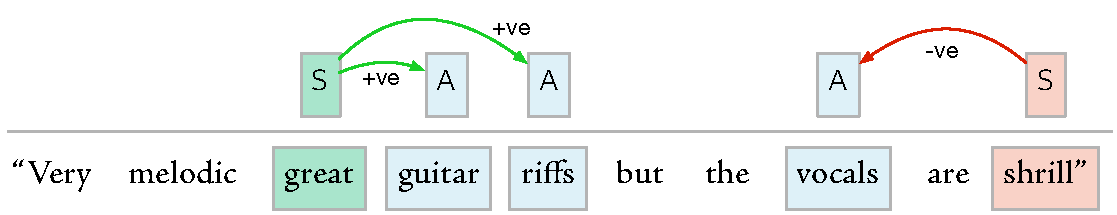
\includegraphics[width=\columnwidth]{ch05_musicology_pics/annotation_sample2}
\caption{A sentence from a sample review annotated with opinion and aspect pairs.}
\label{fig:musicology:annotatedreview}
\end{figure}

\subsection{Experiments}
\label{sec:musicology:experiments}

We carried out a study of the evolution of music criticism from two different temporal standpoints. Specifically, we consider when the review was written and, in addition, when the album was first published. We define the sentiment score of a review as the average score of all aspects in the review. Since we have sentiment information available for each review, we first computed an average sentiment score for each year of review publication (between 2000 and 2014). In this way, we may detect any significant fluctuation in the evolution of affective language during the 21st century. Then, we also calculated an average sentiment score by year of album publication. This information is complemented with the averages of the Amazon rating scores.

In what follows, we show visualizations for sentiment scores and correlation with ratings given by Amazon users, according to these two different temporal dimensions. Although arriving to musicological conclusions is out of the scope of this paper, we provide \textit{food for thought} and present the readers with hypotheses that may explain some of the facts revealed by these data-driven trends.

\begin{figure*}[ht!]
    \centering
    \begin{subfigure}{.32\textwidth}
        \centering
        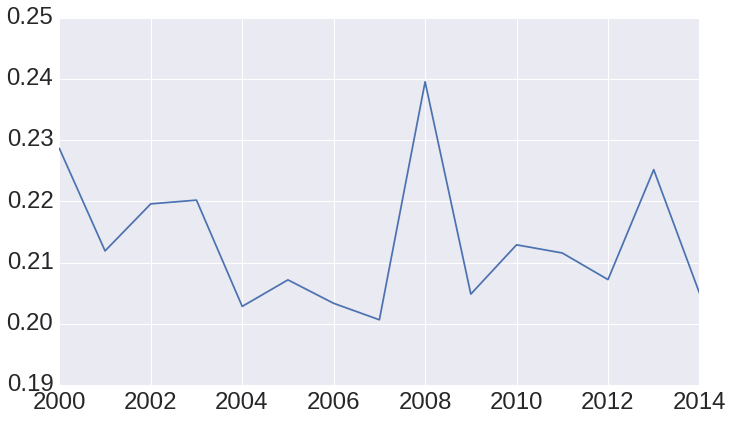
\includegraphics[width=.9\linewidth]{ch05_musicology_pics/all_average.png}
        \caption{Sentiment}
        \label{fig:musicology:avgSentReview}
    \end{subfigure}
    \begin{subfigure}{.32\textwidth}
        \centering
        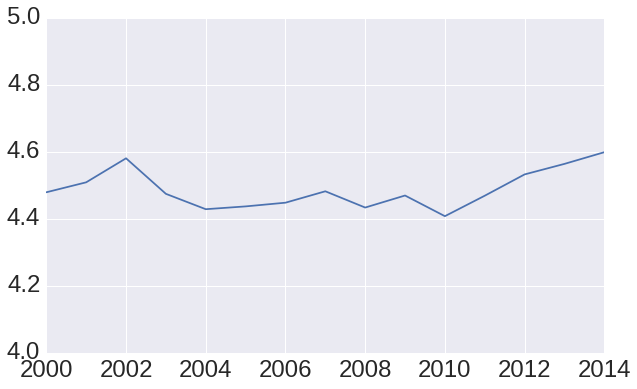
\includegraphics[width=.9\linewidth]{ch05_musicology_pics/avg_score.png}
        \caption{Rating}
        \label{fig:musicology:avgRatingReview}
    \end{subfigure}
    \begin{subfigure}{.32\textwidth}
        \centering
        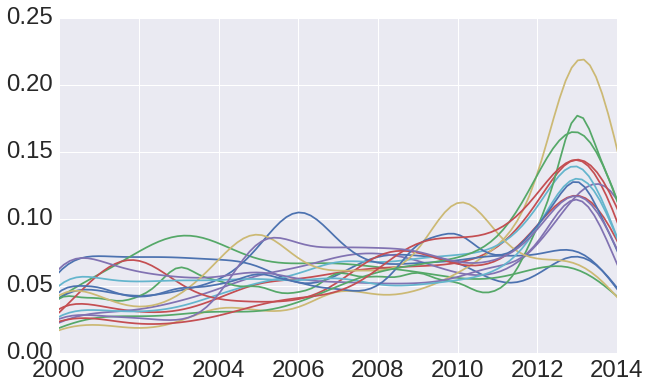
\includegraphics[width=.9\columnwidth]{ch05_musicology_pics/kde.png}
        \caption{Kernel density est.}
        \label{fig:musicology:kde}
    \end{subfigure}
    \begin{subfigure}{.32\textwidth}
        \centering
        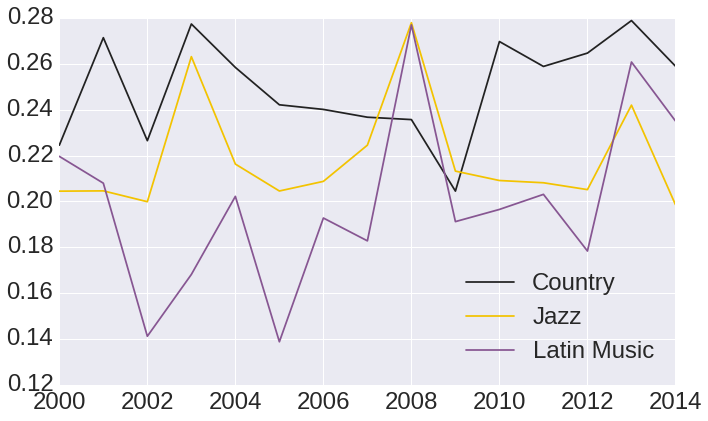
\includegraphics[width=.9\linewidth]{ch05_musicology_pics/genres_average.png}
        \caption{Sentiment by genre}
        \label{fig:musicology:avgSentReviewGenres}
    \end{subfigure}
    \begin{subfigure}{.32\textwidth}
        \centering
        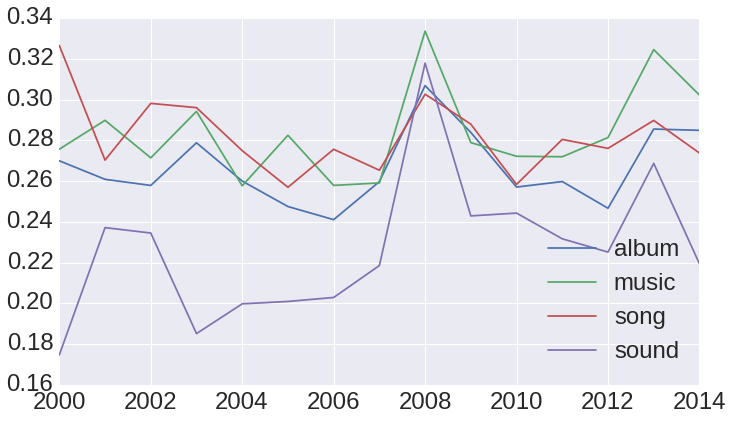
\includegraphics[width=.9\linewidth]{ch05_musicology_pics/main_aspects.png}
        \caption{Sentiment by aspect}
        \label{fig:musicology:avgSentReviewAspects}
    \end{subfigure}
    \begin{subfigure}{.32\textwidth}
        \centering
        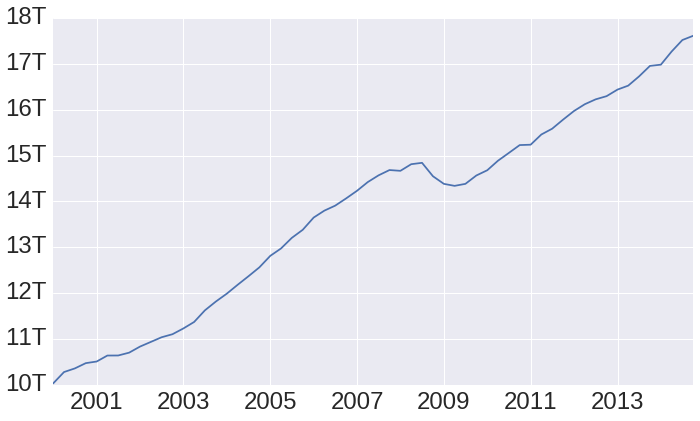
\includegraphics[width=.8\linewidth]{ch05_musicology_pics/gdp2.png}
        \caption{USA GDP trend}
        \label{fig:musicology:gdp}
    \end{subfigure}
 
   \begin{subfigure}{.32\textwidth}
        \centering
        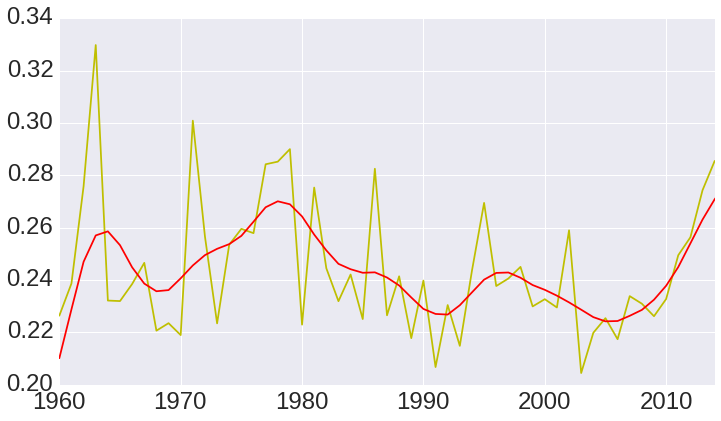
\includegraphics[width=.9\textwidth]{ch05_musicology_pics/sentiment_release_trend.png}
        \caption{Sentiment}
        \label{fig:musicology:avgSentimentRelease}
    \end{subfigure}
    \begin{subfigure}{.32\textwidth}
        \centering
        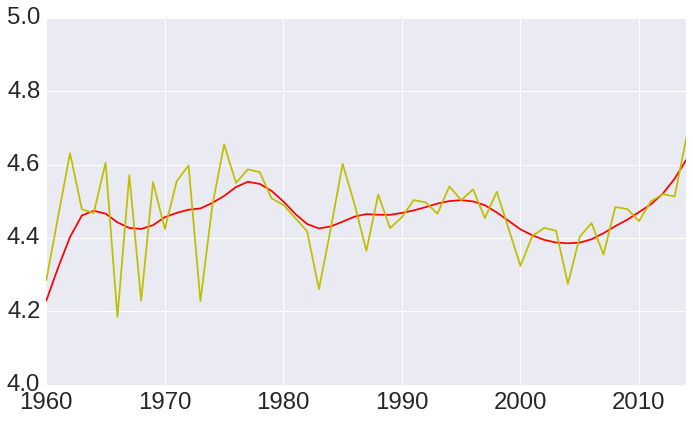
\includegraphics[width=.9\textwidth]{ch05_musicology_pics/rating_release_trend.png}
        \caption{Rating}
        \label{fig:musicology:avgRatingRelease}
    \end{subfigure}
    \begin{subfigure}{.32\textwidth}
        \centering
        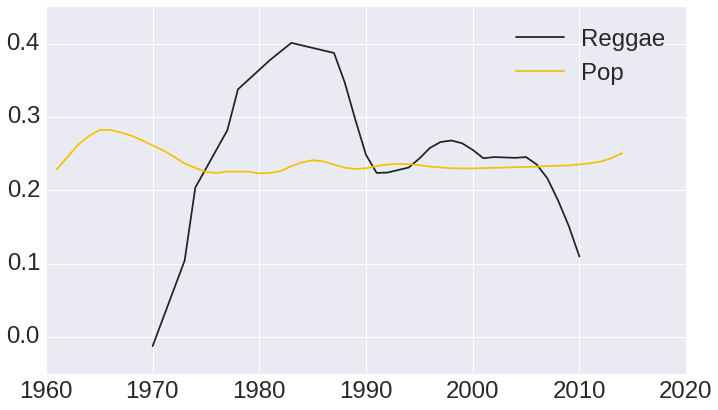
\includegraphics[width=.9\columnwidth]{ch05_musicology_pics/genres_release_trend.png}
        \caption{Sentiment by genre}
        \label{fig:musicology:avgSentimentGenresRelease}
    \end{subfigure}
    %\caption{Sentiment and rating averages by review publication year (a and b); GDP trend in USA from 2000 to 2014 (c), and sentiment and rating averages by album publication year (d, e and f)}
    \caption{Sentiment and rating averages by review publication year (a, b d and e); Kernel density estimation of the distribution of reviews by year (c); GDP trend in USA from 2000 to 2014 (f), and sentiment and rating averages by album publication year (g, h and i)}
\end{figure*}

\subsubsection{Evolution by review publication year}
\label{sec:musicology:evolution-review}

We applied sentiment and rating average calculations to the whole MARD dataset, grouping album reviews by year of publication of the review. Figure \ref{fig:musicology:avgSentReview} shows the average of the sentiment scores of all the reviews published in a specific year, whilst Figure~\ref{fig:musicology:avgRatingReview} shows average review ratings per year. At first sight, we do not observe any correlation between the trends illustrated in the figures. However, the sentiment curve (Figure~\ref{fig:musicology:avgSentReview}) shows a remarkable peak in 2008, a slightly lower one in 2013, and a low between 2003 and 2007, and also between 2009 and 2012. Figure~\ref{fig:musicology:kde} shows the kernel density estimation of the distribution of reviews by year of the 16 genres. The shape of these curves suggest that the 2008 peak in the sentiment score is not related to the number of reviews published that year. The peak persists if we construct the graphs with the average sentiment associated with the most repeated aspects in text (Figure \ref{fig:musicology:avgSentReviewAspects}). 
It is not trivial to give a proper explanation of this variations on the average sentiment. We speculate that these curve fluctuations may suggest some influence of economical or geopolitical circumstances in the language used in the reviews, such as the 2008 election of Barack Obama as president of the US. As stated by the political scientist Dominique Mo\"{i}si in \cite{Moisi2010}:

\begin{displayquote}\small{
In November 2008, at least for a time, hope prevailed over fear. The wall of racial prejudice fell as surely as the wall of oppression had fallen in Berlin twenty years earlier [...] Yet the emotional dimension of this election and the sense of pride it created in many Americans must not be underestimated.}
\end{displayquote}

If we calculate the sentiment evolution curve for the different genres (see Figure~\ref{fig:musicology:avgSentReviewGenres}), we observe that 2008 constitutes an all-time-high for almost all genres. It is remarkable that genres traditionally related to more diverse communities such as Jazz and Latin Music experience such an increase, whilst other genres such as Country do not.

Another factor that might be related to the positiveness in use of language is the economical situation. After several years of continuous economic growth, in 2007 a global economic crisis started\footnote{\url{https://research.stlouisfed.org}}, whose consequences were visible in the society after 2008 (see Figure~\ref{fig:musicology:gdp}). In any case, further study of the different implied variables is necessary to reinforce any of these hypotheses.

%Assuming that a vast majority of reviewers are North American (we do not have this information available), as the dataset was originally gathered from Amazon US, these trends may be explained with the 2008 election of president Barack Obama as president of the US. As stated by Dominique Mo\"{i}si in \cite{Moisi2010}:
%We assume that a vast majority of reviewers should be from the United States, as the dataset was originally gathered from the American version of the Amazon website.  
%Starting from this assumption, an important event happened in 2008 which affected not only United States citizens but the entire world, the election of Barak Obama as the President of the United Sates. As stated by Dominique Moïsi in \cite{Moisi2010}:



%Another factor that might be related to the positiveness in use of language is the economical situation. After several years of continuous economic growth, in 2007 a global economic crisis started, originated by the subprime mortgage crisis, whose consequences were more visible in the society from 2009 to 2013\footnote{\url{https://research.stlouisfed.org}}, as shown in Figure~\ref{fig:musicology:gdp}. %Following this hypothesis, the abrupt decrease of positiveness right after 2008 and its recovery by 2013 might be related to this. 
%In any case, further study of the different implied variables is necessary to reinforce any of these hypotheses.
    

%\begin{figure}
%    \centering
%    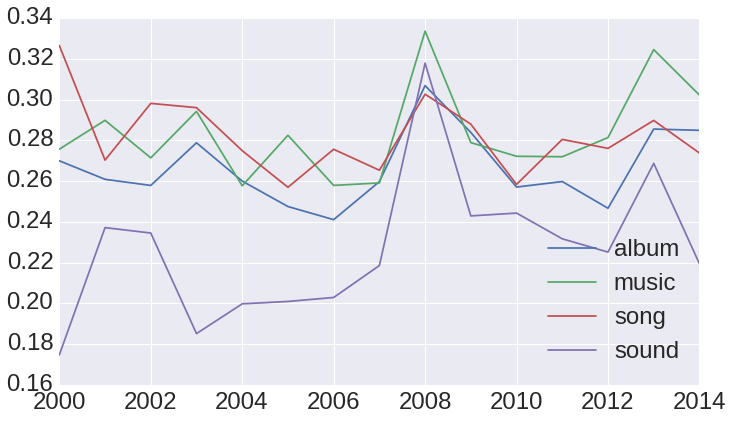
\includegraphics[width=.6\columnwidth]{ch05_musicology_pics/main_aspects.png}
%    \caption{Average sentiment of main aspects across genres by review year}
%    \label{fig:musicology:avgSentimentGenresReview}
%\end{figure}


\subsubsection{Evolution by album publication year}
\label{sec:musicology:evolution-album}

In this case, we study the evolution of the polarity of language by grouping reviews according to the album publication date. This date was gathered from MusicBrainz, meaning that this study is conducted on the ~42,1\% of the MARD that was successfully mapped. We compared again the evolution of the average sentiment polarity (Figure~\ref{fig:musicology:avgSentimentRelease}) with the evolution of the average rating (Figure~\ref{fig:musicology:avgRatingRelease}). Contrary to the results observed by review publication year, here we observe a strong correlation between ratings and sentiment polarity. To corroborate that, we computed first a smoothed version of the average graphs, by applying 1-D convolution (see line in red in Figures~\ref{fig:musicology:avgSentimentRelease} and \ref{fig:musicology:avgRatingRelease}). Then we computed Pearson's correlation between smoothed curves, obtaining a correlation $r = 0.75$, and a p-value $p \ll 0.001$. This means that in fact there is a strong correlation between the polarity identified by the sentiment analysis framework in the review texts, and the rating scores provided by the users. This correlation reinforces the conclusions that may be drawn from the sentiment analysis data. %, and reinforces the idea of averaging local sentiment scores as a measure of polarity in a review. %These sentiment scores might be used as an important feature for a rating prediction task.

To further dig into the utility of this polarity measure for studying genre evolution, we also computed the smoothed curve of the average sentiment by genre, and illustrate it with two idiosyncratic genres, namely \textit{Pop} and \textit{Reggae} (see  Figure~\ref{fig:musicology:avgSentimentGenresRelease}). We observe in the case of \textit{Reggae} that there is a time period where reviews have a substantial use of a more positive language between the second half of the 70s and the first half of the 80s, an epoch which is often called the golden age of \textit{Reggae} \citep{alleyne2012encyclopedia}. This might be related to the publication of Bob Marley albums, one of the most influential artists in this genre, and the worldwide spread popularity of reggae music. In the case of \textit{Pop}, we observe a more constant sentiment average. However, in the 60s and the beginning of 70s there are higher values, probably consequence by the release of albums by The Beatles. These results show that the use of sentiment analysis on music reviews over certain timelines may be useful to study genre evolution and identify influential events.


\section{Conclusions}
\label{sec:musicology:conclusions}

In this Chapter we have shown two different use cases in the context of making sense of large amounts of music related documents from a musicological perspective. (1) A culture-specific music knowledge base has been created, applying a process of automatic knowledge curation, which combines information coming from different data sources. In addition, the knowledge base has been enriched with content extracted directly from unstructured texts by using a custom entity linking system. A methodology to build knowledge graphs is described and tested for computing artist relevance ranking. Evaluation shows high correlation between the obtained ranking of artists and the opinion of a flamenco expert. 
%(2) an analysis on the evolution of Music Digital Libraries based on recent technology advancements have been reported. We pointed out that Music Digital Libraries are still in an early stage of development compared to latest developments on Web search. In addition, we proposed a methodology to exploit knowledge implicit in Digital Library documents, which has been applied on a corpus of artist biographies gathered from the New Grove Dictionary. 
(2) A diachronic study of the sentiment polarity expressed in customer reviews from two different standpoints has been presented. First, an analysis by year of review publication suggests that geopolitical events or macro-economical circumstances may influence the way people speak about music. Second, an analysis by year of album publication shows how sentiment analysis can be useful to study the evolution of music genres. Moreover, according to the observed trend curves, we can state that we are now in one of the happiest periods of the recent history of music. 

In conclusion, the main contribution of the work presented in this chapter is a demonstration of the utility of applying systematic linguistic processing on texts about music. Although further work is necessary to elaborate on the hypotheses or claims that may be derived from purely data-driven analyses, the proposed methodologies have shown their suitability in the quest of knowledge discovery from large amounts of documents, which may be highly useful for musicologists and humanities researchers in general.

\cleartorecto%!TEX root = ../thesis_a4.tex

\part{Knowledge-based Approaches}
\label{part:knowledge-based}

\chapter{Entity Linking for Artist Similarity and Genre Classification}
\label{sec:similarity}

\section{Introduction}\label{sec:similarity:introduction} %Todos

This chapter describes several methods for the semantic enrichment of music documents using Entity Linking and their application in the context of two widely studied MIR tasks, artist similarity and music genre classification. 
First, a method for computing semantic similarity at document-level is presented. The cornerstone of this work is the intuition that semantifying and formalizing relations between entities in documents (both at in-document and cross-document levels) can represent the relatedness of two documents. Specifically, in the task of artist similarity, this derives in a measure to quantify the degree of relatedness between two artists by looking at their biographies. The evaluation results indicate that semantic based apporaches clearly outperform a baseline based on shallow word co-occurrence metrics.
%Our experiments start with a preprocessing step which involve Entity Linking over artist biographical texts.
%Then, a knowledge representation is derived from the detected entities in the form of a semantic graph or a mapping to a vector-space model.
%Finally, different similarity measures are applied to a benchmarking dataset. The evaluation results indicate that some approaches presented in this chapter clearly outperform a baseline based on shallow word co-occurrence metrics.
%Source code and datasets are available online\footnote{\url{http://mtg.upf.edu/downloads/datasets/semantic-similarity}}.
%Second, we explore the contribution of such features to the Music Genre classification task, consisting in, given a song or album review, predict the genre it belongs to.
Second, we perform experiments on music genre classification, exploring a variety of feature types, including semantic features obtained through entity linking, sentimental features  and acoustic features. These experiments show that modeling semantic information contributes to outperforming strong bag-of-words baselines. 

The remainder of this chapter is structured as follows: Section \ref{sec:similarity:similarity} describes a methodology for computing artist similarity from artist biographies using semantic information. Within this section, different types of knowledge representations and similarity measures are described. Then, the settings in which experiments were carried out together with the evaluation metrics used are presented. Finally, evaluation results are presented and the performance of our method discussed. Section \ref{sec:similarity:classification} describes a methodology for computing music genre classification using album reviews. In this section, the dataset of music reviews used is first described. Then, the different types of features are illustrated. An experiment on genre classification is performed and results are discussed.
Finally Section \ref{sec:similarity:conclusion} summarizes the main topics covered in this chapter.

\section{Artist Similarity}
\label{sec:similarity:similarity}

We propose a method proposed for leveraging semantic information in artist biographies. The method can be divided in three main steps, as depicted in Fig~\ref{fig:similarity:methodology}.
The first step performs entity linking. In this case we used Babelfy \cite{Moroetal2014b} through ELVIS (see Section~\ref{sec:linking:elvis}) to identify and link entity mentions in the biographies. Babelfy provides BabelNet URIs, and ELVIS enrich the information of every identified entity with DBpedia URIs, DBpedia Ontology types, and Wikipedia categories.
We opted to use Babelfy for consistency purposes, as in a later step we exploit \textit{SensEmbed}~\cite{Iacobaccietal2015}, a vector space representation of concepts based on BabelNet \cite{Navigli2010}. Moreover, the use of a single tool across approaches guarantees that the evaluation will only reflect the appropriateness of each one of them, and in case of error propagation all the approaches will be affected the same.
The second step derives a semantically motivated knowledge representation from the named entity mentions. This can be achieved by exploiting natural language text as anchor between entities, or by incorporating semantic information from an external knowledge base. In the latter case, a document is represented either as a semantic graph or as a set of vectors projected on a vector space, which allows the use of well known vector similarity metrics.
Finally, the third step computes semantic similarity between documents (artist biographies in our case). This step can take into consideration semantic similarity among entity mentions in document pairs, or only the structure and content of the semantic graph.

%The following sections provide a more detailed description of each one of these steps, along with all the approaches we have considered in each step.
%A schema of the workflow we propose is shown in.

\begin{figure}[!htp]
\centerline{\framebox{
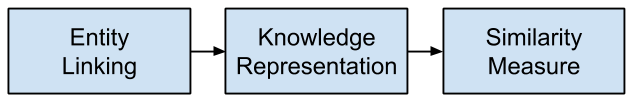
\includegraphics[width=0.75\columnwidth]{ch06_similarity_pics/methodology.png}}}
\caption{Workflow of the proposed method.}
\label{fig:similarity:methodology}
\end{figure}

%\subsection{Entity Linking} %Luis
%
%Entity linking is the task to associate, for a given candidate textual fragment, the most suitable entry in a reference Knowledge Base (KB) \cite{Moroetal2014b}. It encompasses similar subtasks such as Named Entity Disambiguation \cite{BunescuandPasca2006}, which is precisely linking mentions to entities to a KB, or Wikification \cite{MihalceaandCsomai2007}, specifically using Wikipedia as KB.

%We considered several state-of-the-art entity linking tools, including Babelfy \cite{Moroetal2014b}, TagMe \cite{Ferraginaetal2010}, Agdistis \cite{Usbecketal2014} and DBPedia Spotlight \cite{Mendes2011}. However we opted to use the first one for consistency purposes, as in a later step we exploit \textit{SensEmbed}~\cite{Iacobaccietal2015}, a vector space representation of concepts based on BabelNet \cite{Navigli2010}. Moreover, the use of a single tool across approaches guarantees that the evaluation will only reflect the appropriateness of each one of them, and in case of error propagation all the approaches will be affected the same.

%Babelfy \cite{Moroetal2014b} is a state-of-the-art system for entity linking and word sense disambiguation based on non-strict identification of candidate meanings (i.e. not necessarily exact string matching), together with a graph based algorithm that traverses the BabelNet graph and selects the most appropriate semantic interpretation for each candidate.

\subsection{Knowledge Representation}\label{sec:similarity:knowledge_representations}

\subsubsection{Relations Graph}\label{sec:similarity:rel_graph} %Moha

%Relation extraction has been defined as the process of identifying and annotating relevant semantic relations between entities in text \cite{JiangZhai2007}. 
In order to exploit the semantic relations between entities present in artist biographies, we applied the method defined in Chapter~\ref{sec:kb} for relation extraction in the music domain. The method basically consists of three steps. First, entities are identified in the text by applying entity linking. Second, relations between pairs of entities occurring in the same sentence are identified and filtered by analyzing the structure of the sentence, which is obtained by running a syntactic parser based on the formalism of dependency grammar~\cite{Bohnet2010}. Finally, the identified entities and relations are modeled as a knowledge graph.
%connects pairs of entities via labeled relations.
%This kind of extracted knowledge graphs may be useful for music recommendation \cite{Sordo2015}, as recommendations can be conveyed to users by means of natural language. 
We apply this methodology to the problem of artist similarity, by creating a graph that connects the entities detected in every artist biography. We call this approach RG (relations graph). Figure~\ref{fig:similarity:relation} shows the expected output of this process for a single sentence.
%Thus, two artists may be related through different paths of entities, and with different path lengths.

\begin{figure}[!htp]
\centerline{
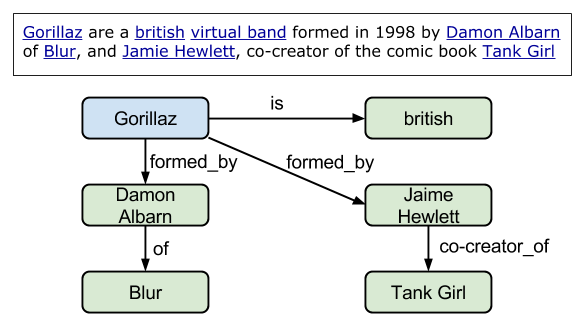
\includegraphics[width=0.95\columnwidth]{ch06_similarity_pics/RelationGraph.png}}
\caption{Relation graph of a single sentence}
\label{fig:similarity:relation}
\end{figure}


\subsubsection{Semantically enriched graph}\label{sec:similarity:semantic_enriched_graph} %Sergio

A second approach is proposed using the same set of linked entities. However, instead of exploiting natural language text, we use semantic information from the referenced knowledge base to enrich the semantics of the linked entities. We follow a semantic enrichment process similar to the one described in Section~\ref{sec:musicology:relevance}. We use semantic information coming from DBpedia\footnote{\url{http://dbpedia.org}}. DBpedia resources are generally classified using the DBpedia Ontology, which is a shallow, cross-domain ontology based on the most common infoboxes of Wikipedia. DBpedia resources are categorized using this ontology among others (e.g. Yago, schema.org) through the \texttt{rdfs:type} property. In addition, each Wikipedia page may be associated with a set of Wikipedia categories, which link chapters under a common topic. DBpedia resources are related to Wikipedia categories through the property \texttt{dcterms:subject}.

We take advantage of these two properties to build our semantically enriched graph.
We consider three types of nodes for this graph: 1) artist entities obtained by matching the artist names to their corresponding DBPedia entry; 2) named entities detected by the entity linking step; and 3) Wikipedia categories associated to all the previous entities.
Edges are then added between artist entities and the named entities detected in their biographies, and between entities and their corresponding Wikipedia categories.
For the construction of the graph, we can select all the detected named entities, or we can filter them out according to the information related to their \texttt{rdfs:type} property. A set of six types was selected, including \textit{Artist}, \textit{Band}, \textit{Work}, \textit{Album}, \textit{MusicGenre}, and \textit{Person}, which we consider more appropriate to semantically define a musical artist.

From the previous description, we define five variants of this approach. The first variant, which we call AEC (Artists-Entities-Categories), considers all 3 types of nodes along with their relations (as depicted in Figure~\ref{fig:similarity:enriched}). The second variant, named AE (Artists-Entities) ignores the categories of the entities. The third and fourth variant, named AEC-FT and AE-FT, are similar to the first and second variant, respectively, except that the named entities are filtered using the above mentioned list of 6 entity types. Finally, the fifth variant, EC, ignores the artist entities of node type 1.

\begin{figure}[!htp]
\centerline{
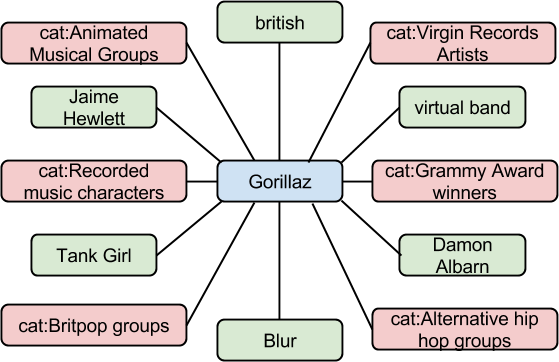
\includegraphics[width=0.95\columnwidth]{ch06_similarity_pics/EnrichedGraph1.png}}
\caption{Semantically enriched subgraph of the same sentence from Figure~\ref{fig:similarity:relation}, variant AEC with h=1}
\label{fig:similarity:enriched}
\end{figure}

%First, artist entities are added to the graph as nodes. For every artist, all entities detected in its biography are added to the graph as nodes, and connected through an edge to the artist entity. For every added entity, its associated Wikipedia categories are retrieved and added to the graph as nodes. Every entity is attached to its associated categories though and edge. Thus, a graph of artists, linked entities and semantic categories is finally generated.
%
%A second version of the graph is proposed. Instead of adding all detected entities, we filter them out according to the information related to their \texttt{rdfs:type} property. A set of six types was selected, including \textit{artist}, \textit{band}, \textit{work}, \textit{album}, \textit{musicgenre}, and \textit{person}. These types address to the entities that we consider more appropriate to semantically define a musical artist. Hence, a filtered version of the graph is built by selecting entities only of the specified types, and their corresponding categories.
%
%For evaluation purposes, we created two more versions of the graph. Both versions follow the same graph creation process, but ignoring the last step of adding categories. Though, the graphs includes only artist entities and detected entities. One version includes all detected entities, and the other only entities of the specified types.

\subsubsection{Sense embeddings}\label{sec:similarity:sense_embeddings}

The semantic representation used in this approach is based on SensEmbed \cite{Iacobaccietal2015}. SensEmbed is a vector space semantic representation of words similar to word2vec \cite{Mikolovetal2013},
%with the aggregated value than instead of plain text words,
where each vector represents a BabelNet synset and its lexicalization. Let $A$ be the set of artist biographies in our dataset. Each artist biography $a \in A$ is converted to a set of disambiguated concepts $\text{Bfy}_{a}$ after running Babelfy over it.

\subsection{Similarity approaches}

\subsubsection{SimRank} %Moha

SimRank is a similarity measure based on an simple graph-theoretic model \cite{jeh2002simrank}. The intuition is that two nodes are similar if they are referenced by similar nodes. In particular we use the definition of bipartite SimRank \cite{jeh2002simrank}. We build a bipartite graph with named entities and their corresponding Wikipedia categories (the EC variant from Section~\ref{sec:similarity:semantic_enriched_graph}). The similarity between two named entities (say $p$ and $q$) is computed with the following recursive equation:

\begin{equation}
s(p,q) = \frac{C}{|O(p)||O(q)|} \sum_{i=1}^{|O(p)|} \sum_{j=1}^{|O(q)|} s(O_i(p), O_j(q))
\end{equation}

where $O$ denotes the out-neighboring nodes of a given node and $C$ is a constant between 0 and 1. For $p = q$, $s(p,q)$ is automatically set up to $1$.
Once the similarity between all pairs of entities is obtained, we proceed to calculate the similarity between pairs of artists (say $a$ and $b$) by aggregating the similarities between the named entities identified in their biographies, as shown in the following formula:

\begin{equation}
\footnotesize
sim(a,b) = Q(a,b) \frac{1}{N} \sum_{e_a \in a} \sum_{e_b \in b} s(e_a, e_b)\quad \text{if}\ s(e_a, e_b) \geq 0.1
\end{equation}

where $s$ denotes the SimRank of entities $e_a$ and $e_b$ and $N$ is the number of ($e_a$, $e_b$) pairs with $s(e_a, e_b) \geq 0.1$. This is done to filter out less similar pairs.
%We only consider pairs of entities with $s(e_a, e_b) \geq 0.1$. This is done to filter out less similar pairs.
%
Finally, $Q(a,b)$ is a normalizing factor that accounts for the pairs of artists with more similar entity pairs than others.
%, and it is computed as follows:

%\begin{equation}
%Q(a,b) = \frac{N(a,b)^{\alpha-1}}{max\_N(a)^{\alpha}}
%\end{equation}
%
%where $N(a,b)$ is the number of ($e_a$, $e_b$) pairs with $s(e_a, e_b) \geq 0.1$, and $max\_N(a)$ is the largest value of $N$ for artist $a$.
%$\alpha$ is a parameter between 0 and 1. We empirically set $\alpha = 0.6$.


\subsubsection{Maximal common subgraph}\label{sec:similarity:method:sim:mcs} %Sergio

Maximal common subgraph (MCS) is a common distance measure on graphs. It is based on the maximal common subgraph of two graphs. MCS is a symmetric distance metric, thus $d(A,B)=d(B,A)$. It takes structure as well as content into account. According to \cite{Bunke1998}, the distance between two non empty graphs $G_{1}$ and $G_{2}$ is defined as

\begin{equation}
d(G_{1},G_{2}) = 1 - \cfrac{| mcs(G_{1},G_{2}) |}{max(|G_{1}|,|G_{2}|)}
\end{equation}

It can also be seen as a similarity measure $s$, assuming that $s=1-d$, as applied in \cite{Lux2005}. To compute this similarity measure we need to have a graph for each artist. This can be achieved by finding subgraphs in the graph approaches defined in Section~\ref{sec:similarity:knowledge_representations}. A subgraph will include an artist entity node and its neighboring nodes.
Furthermore, we apply the notion of h-hop item neighborhood graph defined in \cite{ODMD14a} to a semantic graph. Let $G=(E,P)$ be an undirected graph where $E$ represent the nodes (entities), and $P$ the set of edges with $P \subseteq E \times E$. For an artist item $a$ in $G$, its h-hop neighborhood subgraph $G^{h}(a)=(E^{h}(a),P^{h}(a))$ is the subgraph of $G$ formed by the set of entities that are reachable from $a$ in at most h hops, according to the shortest path. %An example of a 2-hop item neighborhood graph of an artist is shown in ~Fig.
Following this approach, we obtain an h-hop item neighborhood graph for each artist node of the semantic graph. Then, maximal common subgraph is computed between each pair of h-hop item neighborhood graphs. For each artist, the list of all similar artists ordered from the most similar to the less one is finally obtained.

\subsubsection{Cumulative cosine similarity} %Luis

%The semantic representation used in this approach is based on SensEmbed \cite{Iacobaccietal2015}, a vector space semantic representation of words similar to word2vec \cite{Mikolovetal2013}, with the aggregated value than instead of plain text words, each vector represents a BabelNet synset and its lexicalization. Specifically, the following steps are performed: (1) Let $A$ be the set of artist biographies in our dataset, in which each artist biography $a \in A$ is converted to a set of disambiguated concepts $\text{Bfy}_{a}$ after running Babelfy over it. (2)
For each pair of concepts $c \in \text{Bfy}_{a}$ and $c^{\prime} \in \text{Bfy}^{\prime}_{a}$ (as defined in Section \ref{sec:similarity:sense_embeddings}), we are interested in obtaining the similarity of their closest senses. This is achieved by first deriving the set of associated vectors $V_c$ and $V_{c^{\prime}}^{\prime}$ for each pair of concepts $c,\,c^{\prime}$, and then optimizing

\begin{equation}
\operatorname{max}_{v_c \in V_c , v_{c^{\prime}}^{\prime} \in V_{c^{\prime}}^{\prime}}
\left( \frac{v_c \times v_{c^{\prime}}^{\prime}}{\left\vert\left\vert{v_c}\right\vert\right\vert \left\vert\left\vert{v_{c^{\prime}}^{\prime}}\right\vert\right\vert } \right)
\end{equation}

i.e. computing cosine similarity between all possible senses (each sense represented as a vector) in an all-against-all fashion and keeping the highest scoring similarity score for each pair. Finally, the semantic similarity between two artist biographies is simply the average among all the cosine similarities between each concept pair.

\subsection{Experimental Setup}
\label{sec:similarity:experimentalsetup}

To evaluate the accuracy of the proposed approaches we designed an experimental evaluation over two datasets. The first dataset contains 2,336 artists and it is evaluated using the list of similar artists provided by the Last.fm API as a ground truth. The second dataset contains 188 artists, and it is evaluated against user similarity judgements from the MIREX Audio Music Similarity and Retrieval task.
%More information, as well as data, can be accessed online at http://music-ir.org/mirex/wiki/MIREX\_HOME} Audio and Music Similarity evaluation dataset.
Apart from the defined approaches, a pure text-based approach for document similarity is added to act as a reference for the obtained results.

%\subsection{Datasets}

\subsubsection{Last.fm dataset}\label{sec:similarity:lastfm_dataset}

A dataset of 2,336 artist biographies was gathered from Last.fm. The artists in this dataset share a set of restrictions.
Their biography has at least 500 characters and is written in English.
All of the artists have a correspondent Wikipedia page, and we have been able to mapped it automatically, obtaining the DBpedia URI of every artist.
For every artist, we queried the getSimilar method of the Last.fm API and obtained an ordered list of similar artists. Every artist in the dataset fulfills the requirement of having at least 10 similar artists within the dataset.
We used these lists of similar artists as the ground truth for our evaluation.
%As the list contains at least 10 similar artists within the dataset, we can evaluate top-10 similarity.

\subsubsection{MIREX dataset} %Moha

To build this dataset, the gathered artists from Last.fm
%(without the application of the last restriction mentioned in Section~\ref{sec:similarity:lastfm_dataset})
were mapped to the MIREX Audio Music Similarity task dataset. The AMS dataset (7,000 songs from 602 unique artists) contains human judgments of song similarity. According to~\cite{Schedl2013}, the similarity between two artists can be roughly estimated as the average similarity between their songs. We used the same approach in~\cite{Schedl2013}, that is, two artists were considered similar if the average similarity score between their songs was at least 25 (on a fine scale between 0 and 100).

%to use this dataset for artist similarity evaluation.
After the mapping, we obtained an overlap of 268 artists.
%We used this dataset of 268 artists to compute similarity using the different approaches.
As we want to evaluate Top-10 similarity, every artist in the ground truth dataset should have information of at least 10 similar artists. However, not every artist in the MIREX evaluation dataset fulfills this requirement. Therefore, after removing the artists with less than 10 similars, we obtained a final dataset of 188 artists, and used it for the evaluation.

\subsubsection{Baseline}
In order to assess the goodness of our approaches, we need to define a baseline approach with which to compare to. The baseline used in this chapter is a classic vector-based model approach used in many Information Retrieval systems. A text document is represented as a vector of word frequencies (after removing English stopwords and words with less than 2 characters), and a matrix is formed by aggregating all the vectors. The word frequencies in the matrix are then re-weighted using TF-IDF, and finally latent semantic analysis (LSA) \cite{Deerwesteretal1990} is used to produce a vector of concepts for each document. The similarity between two documents can be obtained by using a cosine similarity over their corresponding vectors.

\begin{table}[ht!]
\small
\centering
	\begin{tabular}{  lllll }
 	\toprule
& \multicolumn{2}{c}{Precision@N} & \multicolumn{2}{c}{nDCG@N} \\
\cmidrule(lr){2-3}
\cmidrule(lr){4-5}
	Approach variants & N=5 & N=10 & N=5 & N=10 \\
	\midrule
LSA & 0.100 & 0.169 & 0.496 & 0.526 \\
RG MCS 1-hop & 0.059 & 0.087 & 0.465 & 0.476 \\
RG MCS 2-hop & 0.056 & 0.101 & 0.433 & 0.468 \\
AE MCS & 0.106 & 0.178 & 0.503  & 0.517 \\
AE-FT MCS & 0.123 & 0.183 & 0.552 & 0.562 \\
AEC MCS 1-hop & 0.120 & 0.209 & 0.573 & 0.562 \\
AEC MCS 2-hop & 0.086 & 0.160 & 0.550 & 0.539 \\
AEC-FT MCS 1-hop & \textbf{0.140} & \textbf{0.218} & \textbf{0.588} & \textbf{0.578} \\
AEC-FT MCS 2-hop & 0.100 & 0.160 & 0.527 & 0.534 \\
EC SimRank & 0.097& 0.171 &  0.509 & 0.534 \\
SE Cosine & 0.095 & 0.163 & 0.454 & 0.484 \\
\bottomrule	
	\end{tabular}
	\caption{Precision and normalized discounted cumulative gain for Top-N artist similarity using the MIREX dataset (N=\{5, 10\})}	
	\label{tbl:similarity:res_mirex}
\end{table}

\begin{table}
\small
\centering
	\begin{tabular}{ lllll }
 	\toprule
	& \multicolumn{2}{c}{Precision@N} & \multicolumn{2}{c}{nDCG@N} \\
\cmidrule(lr){2-3}
 \cmidrule(lr){4-5}
	Approach variants & N=5 & N=10 & N=5 & N=10 \\
	\midrule
LSA & 0.090 & 0.088 & 0.233 & 0.269 \\
RG MCS 1-hop & 0.055 & 0.083 & 0.126 & 0.149 \\
AE MCS & 0.124 & 0.200 & 0.184 & 0.216 \\
AE-FT MCS & 0.136 & 0.201 & 0.224 & 0.260 \\
AEC MCS 1-hop & 0.152 & 0.224 & 0.277 & 0.297 \\
AEC-FT MCS 1-hop & \textbf{0.160} & \textbf{0.242} & \textbf{0.288} & \textbf{0.317} \\
\bottomrule
	\end{tabular}
	\caption{Precision and normalized discounted cumulative gain for Top-N artist similarity using the Last.fm dataset (N=\{5, 10\})}	
	\label{tbl:similarity:res_lastfm}
\end{table}

\subsubsection{Evaluated approaches}\label{sec:similarity:eval_approaches} %Sergio

From all possible combinations of knowledge representations, similarity measures and parameters, we selected a set of 10 different approach variants. The prefixes AEC, RG and AE refer to the graph representations (see Sections \ref{sec:similarity:rel_graph} and \ref{sec:similarity:semantic_enriched_graph}). %AEC refers to the artist entity categories graph, RG to the graph of relations extracted from text, and AE to a graph with artist entities and named entities.
SE refers to the sense embeddings approach, and LSA to the latent semantic analysis baseline approach. When these prefixes are followed by FT, it means that the entities in the graph have been filtered by type. The second term in the name refers to the similarity measure. MCS refers to maximal common subgraph, and SimRank and Cosine to SimRank and cumulative cosine similarity measures. MCS approaches are further followed by a number indicating the number of h-hops of the neighborhood subgraph.


\begin{table*}[ht!]
\scriptsize
\centering
	\begin{tabular}{ lllllllll }
 	\toprule
& \multicolumn{8}{c}{Genres} \\
\cmidrule(lr){2-9}
	Approach variants & Blues & Country & Edance & Jazz & Metal & Rap & Rock & Overall\\
	\midrule
Ground Truth & 5.78 & 5.46 & 6.88 & 7.04 & 7.10 & 8.68 & 5.17 & 6.53\\
\midrule[.2pt]
LSA & 4.43 & 4.12 & 3.80 & 4.64 & 5.79 & 5.08 & 4.74 & 4.69\\
RG MCS 1-hop & 2.63 & 3.50 & 1.50 & 2.95 & 4.00 & 2.54 & 1.70 &  2.68\\
RG MCS 2-hop & 4.14 & 4.92 & 1.69 & 2.80 & 3.78 & 3.06 & 2.77 & 3.27\\
AE MCS & 5.52 & 5.15 & 4.36 & 7.00 & 4.34 & 5.36 & 4.46 & 5.11\\
AE-FT MCS & 5.43 & 6.12 & 4.16 & 6.20 & 6.32 & 5.36 & 3.77 & 5.26 \\
AEC MCS 1-hop & \textbf{7.22} & 5.92 & 5.24 & 7.12 & 5.48 & 6.92 & 4.86 & 6.02 \\
AEC MCS 2-hop & 4.22 & 3.69 & 4.56 & 6.20 & 4.55 & 4.64 & 4.09 & 4.54 \\
AEC-FT MCS 1-hop & 6.91 & \textbf{6.80} & \textbf{6.04} & \textbf{7.60} & \textbf{6.79} & \textbf{7.12} & \textbf{5.37} & \textbf{6.59} \\
AEC-FT MCS 2-hop & 4.09 & 4.36 & 5.56 & 6.72 & 4.39 & 4.16 & 3.77 & 4.67 \\
EC SimRank & 6.74 & 5.38 & 3.16 & 6.40 & 4.59 & 4.44 & 3.80 & 4.85 \\
SE Cosine & 3.39 & 5.50 & 5.32 & 5.16 & 4.31 & 5.36 & 4.31 & 4.75 \\
\bottomrule	
	\end{tabular}
	\caption{Average genre distribution of the top-10 similar artists using the MIREX dataset. In other words, on average, how many of the top-10 similar artists are from the same genre as the query artist. LSA stands for Latent Semantic Analysis, RG for Relation Graph, SE for Sense Embeddings,  and AE, AEC and EC represent the semantically enriched graphs with Artists-Entities, Artist-Entities-Categories, and Entities-Categories nodes, respectively. As for the similarity approaches, MCS stands for Maximum Common Subgraph.}	
	\label{tbl:similarity:res_genre_distrib}
\end{table*}


\subsubsection{Evaluation measures}

To measure the accuracy of the artist similarity we adopt two standard performance metrics such as Precision@N, and nDCG@N (normalized discounted cumulative gain).
%We applied the metrics as defined in \cite{Steck13} for evaluating recommendation, but adapted to the problem of artist similarity.
Precision@N is computed as the number of relevant items (i.e., true positives) among the top-N items divided by $N$, when compared to a ground truth.
%A relevant item is an item in the list of $N$ similar artists suggested by the system for an artist $a$, that is also in the ground truth list of N similar artists of the same artist $a$.
%Recall@N (R@N) is computed as the ratio between the number of relevant items among the top-N items and the number items in the ground truth list.
Precision considers only the relevance of items, whilst nDCG takes into account both relevance and rank position. Denoting with  $s_{ak}$ the relevance of the item in position $k$ in the Top-N list for the artist $a$, then nDCG@N for $a$ can be defined as:
%%%%%%%%%%%%%%%%%%%%%%%%%%%
\begin{equation}\label{eq:recall}
\text{nDCG@N} = \frac{1 }{\text{IDCG@N}} \sum^N_{k=1} \frac{ 2^{ s_{ak}} -1 }{\log_2 (1+k)}
\end{equation}
%%%%%%%%%%%%%%%%%%%%%%%%%%%
where IDCG@N indicates the score obtained by an ideal or perfect Top-N ranking and acts as a normalization factor. We run our experiments for $N=5$ and $N=10$.
%In Tables~\ref{tbl:similarity:res_mirex} and~\ref{tbl:similarity:res_lastfm} average values of P@N and nDCG@N among all the evaluated artists are shown.

\subsection{Results and discussion}
\label{sec:similarity:results}

We evaluated all the approach variants described in Section~\ref{sec:similarity:eval_approaches} on the MIREX dataset, but only a subset of them on the Last.fm dataset, due to the high computational cost of some of the approaches.
%We initially worked on the MIREX dataset, as the number of artists was smaller and the computation of the algorithms was much faster. However, to ensure the credibility of the results, we applied some of the approach variants in a bigger dataset.

Table~\ref{tbl:similarity:res_mirex} shows the Precision@N and nDCG@N results of the evaluated approaches using the MIREX dataset, while Table~\ref{tbl:similarity:res_lastfm} shows the same results for the Last.fm dataset. We obtained very similar results in both datasets. The approach that gets best performance for every metric, dataset and value of N is the combination of the Artists-Entities-Categories graph filtered by types, with the maximal common subgraph similarity measure using a value of $h=1$ for obtaining the h-hop item neighborhood graphs.

Furthermore, given that the MIREX AMS dataset also provides genre data, we analyzed the distribution of genres in the top-10 similar artists for each artist, and averaged them by genres. The idea is that an artist's most similar artists should be from the same genre as the seed artist.
Table~\ref{tbl:similarity:res_genre_distrib} presents the results. Again, the best results are obtained with the approach that combines the Artists-Entities-Categories graph filtered by types, with the maximal common subgraph similarity measure using a value of $h=1$ for the h-hop item neighborhood graphs.

We extract some insights from these results. First, semantic approaches are able to improve pure text-based approaches. Second, using knowledge from an external knowledge base provides better results than exploiting the relations inside the text. Third, using a similarity measure that exploits the structure and content of a graph, such as maximal common subgraph, overcomes other similarity measures based on semantic similarity among entity mentions in document pairs.


\section{Music Genre Classification}\label{sec:similarity:classification}

In this section we describe an experiment on music genre classification, consisting in, given an album review, predict the genre it belongs to. To this end we explore a variety of feature types, including semantic, sentimental and acoustic features. %First, we briefly describe the dataset used for training and testing, and then we provide a description of the features used for this task.

\subsection{Dataset Description}

Starting from the Multimodal Album Reviews Dataset (MARD) described in Section~\ref{sec:musicology:mard}, our purpose is to create a subset suitable for music genre classification, including 100 albums per genre class. We enforce these albums to be authored by different artists, and that review texts and audio descriptors of their songs are available in MARD. Then, for every album, we selected audio descriptors of the first song of each album as representative sample of the album. From the original 16 genres, 3 of them did not have enough instances complying with these prerequisites (Reggae, Blues and Gospel). This results in a classification dataset composed of 1,300 albums, divided in 13 different genres, with around 1,000 characters of review per album.

In addition to the aspect-based sentiment analysis process applied over the MARD dataset (see Section~\ref{sec:musicology:sentiment}), we applied an Entity Linking process to the selected subset of reviews. In this case, EL was performed taking advantage of TagMe \cite{Ferragina2012} through ELVIS (see Section~\ref{sec:linking:elvis}). TagMe provides for each detected entity, its Wikipedia page id. ELVIS enrich the obtained entities with DBpedia URIs, DBpedia Ontology types, and Wikipedia categories.
%An album may have a number of reviews with different length each. For each album we selected a subset of its reviews and concatenated their texts. We aimed to limit the cumulative length of the selected reviews of each album to 1000 characters approximately, without cropping any reviews. Finally, the average length of text by album in the classification dataset is 649 characters.

\subsection{Features}
\label{sec:similarity:features}
\subsubsection{Textual Surface Features}
We used a standard Vector Space Model representation of documents, where documents are represented as bag-of-words (BoW) after tokenizing and stopword removal. All words and bigrams (sequences of two words) are weighted according to \textit{tf-idf} measure. 

\subsubsection{Semantic Features}

We enriched the initial BoW vectors with semantic information thanks to the application of entity linking. Specifically, for each named entity disambiguated with TagMe, its Wikipedia ID and its associated categories are added to the feature vector, also with \textit{tf-idf} weighting. Wikipedia categories are organized in a taxonomy, so we enriched the vectors by adding one level more of broader categories to the ones provided by ELVIS. Broader categories were obtained by querying DBpedia\footnote{\url{http://dbpedia.org}}.

%We enriched the initial BoW vectors with semantic information thanks to the EL step. The semantic feature vector of an album is conformed by a BoW model where instead of words, there are entity IDs and categories. For every entity detected by Tagme in the album texts, we added to BoW its correspondent Wikipedia ID and the Wikipedia categories associated to this entity. We applied the tfidf measure to the semantic features vector to compute a weight associated to every entity and category for each album.

\subsubsection{Sentiment Features} 

Based on those aspects and associated polarity extracted with the opinion mining framework, with an average number of aspects per review around 37, we follow \cite{Suero2014} and implement a set of sentiment features, namely:

\begin{itemize}
    \item Positive to All Emotion Ratio: fraction of all sentimental features which are identified as positive (sentiment score greater than 0). 
    %Ratio between the positive aspects and all the aspectes identified in the text. We consider an aspect as positive if it has an associated sentiment score greater than 0, and negative if it is below 0. 
    %This feature is given by:
    %\begin{equation}
    %    PosRatio = \frac{PosAspects}{PosAspectes + NegAspects}
    %\end{equation}
    \item Document Emotion Ratio: fraction of total words with sentiments attached. This feature captures the degree of affectivity of a document regardless of its polarity.
    %This feature is designed to capture the degree of affectivity (regardless of polarity) of a document. It is based on the ratio of identified aspects to all words in the document. 
    %\begin{equation}
    %    eRatio = \frac{TotalAspects}{TotalWords}
    %\end{equation}
    \item Emotion Strength: This document-level feature is computed by averaging sentiment scores over all aspects in the document.
    %Emotion Strength: This feature shows the average of the sentiment scores associated to all the identified aspects in a document
    \item F-Score\footnote{Not to be confused with the evaluation metric.}: This feature has proven useful for describing the contextuality/formality of language. It takes into consideration the presence of \textit{a priori} ``descriptive'' POS tags (nouns and adjectives), as opposed to ``action'' ones such as verbs or adverbs.
    
    %It is designed to capture the usage of certain informative part-of-speech categories by looking at their frequency $F$, as follows:
    %\begin{equation}
    %\begin{split}
    %    Fscore = 0.5 * ((nounF+adjF+prepF+artF) \\
%-(pronF+verbF+advF+intF) + 100)
    %\end{split}
    %\end{equation}
\end{itemize}

\subsubsection{Acoustic Features}

Acoustic features are obtained from AB. They are computed using Essentia\footnote{\url{http://essentia.upf.edu/}}. These encompass loudness, dynamics, spectral shape of the signal, as well as additional descriptors such as time-domain, rhythm, and tone \cite{Porter2015}.% For instance, rhythm descriptors refer to beat positions and BPM value, while tonal information includes chroma features, keys and scales .

%Acoustic features, obtained from MB, are computed The set of acoustic features used is provided by AcousticBrainz, which is described in \cite{Porter2015}. These features are computed using the Essentia library\footnote{\url{http://essentia.upf.edu/}}. They are divided into low-level and high-level features. Low-level features encompasses spectral, time-domain, rhythm, and tonal descriptors, whilst high-level are generated after applying data mining and machine learning techniques over low-level features. We only used in our experiments the set of low-level features, which includes features characterizing overall loudness, dynamics, and spectral shape of the signal, rhythm descriptors (including beat positions and BPM value), and tonal information (including chroma features, keys and scales).


\subsection{Baseline approaches}
\label{sec:similarity:baselines}
Two baseline systems are implemented. First, we implement the text-based approach described in \cite{Hu2005} for music review genre classification. In this work, a Na\"{i}ve Bayes classifier is trained on a collection of 1,000 review texts, and after preprocessing (tokenisation and stemming), BoW features based on document frequencies are generated.
The second baseline is computed using the AB framework for song classification \cite{Porter2015}. Here, genre classification is computed using  multi-class support vector machines (SVMs) with a one-vs.-one voting strategy. The classifier is trained with the set of low-level features present in AB. %The dataset is split 80-20\% for training and testing, and accuracy values are obtained after 5-fold cross validation. 
%The second baseline is the well known audio-based approach for genre classification described in \cite{Tzanetakis2002}. Their experiments are performed on the GTZAN dataset, consisting in 1,000 audio files categorized across 10 genres. Given that classification results using this approach are already present in AcousticBrainz, we directly computed the accuracy of these predictions in our dataset. % Al quitar la diferencia entre low y high level features arriba he quitado aqui la ref a high level features. Tampoco se lo que son, asi que si es importante habra q modificarlo.

%We used two different baseline approaches to compare the obtained results. First, we implemented the text-based approach described in \cite{Hu2006} for genre classification of music reviews. In this work, a Multinomial Naive Bayes classifier is applied to a dataset of 1,000 reviews. Review texts are tokenized and stemmized and then document frequency of word tokens is computed and used as feature weight of a bag-of-words vector. We trained and tested the apporach on our dataset of review texts.
%Second, the well known audio-based approach for genre classification described in \cite{Tzanetakis2002} is applied to our dataset. In this work, the classifier is applied to a dataset of 1000 audio files classified into 10 different genres, known as the GTZAN dataset. Given that classification results using this approach are already present in the set of high-level features of AcousticBrainz, we directly computed the accuracy of these predictions in our dataset.


\subsection{Experiments}

\begin{table}[]
\centering
\begin{tabular}{l|r|r|r|}
\cline{2-4}
                                       & \multicolumn{1}{l|}{BoW} & \multicolumn{1}{l|}{BoW+SEM} & \multicolumn{1}{l|}{BoW+SENT} \\ \hline
\multicolumn{1}{|l|}{Linear SVM}       & \textbf{0.629}           & \textbf{0.691}               & \textbf{0.634}                \\ \hline
\multicolumn{1}{|l|}{Ridge Classifier} & 0.627                    & 0.689                        & 0.61                          \\ \hline
\multicolumn{1}{|l|}{Random Forest}    & 0.537                    & 0.6                          & 0.521                         \\ \hline
\end{tabular}
\caption{Accuracy of the different classifiers}
\label{tbl:similarity:classifiers}
\end{table}

We tested several classifiers typically used for text classification, namely Linear SVM, Ridge Classifier and Nearest Centroid, using the implementations provided by the scikit-learn library\footnote{http://scikit-learn.org/}. Among them, Linear SVM has shown better performance when combining different feature sets (see Table~\ref{tbl:similarity:classifiers}). Therefore, we trained a Linear SVM classifier with L2 penalty over different subsets of the features described in Section \ref{sec:similarity:features}, which are combined via linear aggregation. Specifically, we combine the different feature sets into five systems, namely \textbf{BoW} (BoW), \textbf{BoW+Semantic} without broader categories (BoW+SEM), \textbf{BoW+Semantic Broader} with broader categories (BoW+SEMb), \textbf{BoW+Sentiment} (BoW+SENT) and \textbf{BoW+Semantic+Sentiment} (BoW+SEM+SENT). In this way, we aim at understanding the extent to which sentiment and semantic features (and their interaction) may contribute to the review genre classification task. Note that this chapter is focused on the influence of textual features in genre classification, and classification based on acoustic features is simply used as a baseline for comparison. A proper combination of acoustic and textual features in text classification is a challenging problem and would require a deeper study that is out of the scope of this chapter.
The dataset is split 80-20\% for training and testing, and accuracy values are obtained after 5-fold cross validation. 
%As for training and test splits, we first divide the dataset, for each genre, in 80\% for training and 20\% for evaluation, and apply 5-fold cross-validation. We report average numbers across the 5 folds.

\begin{figure}
    \centering
    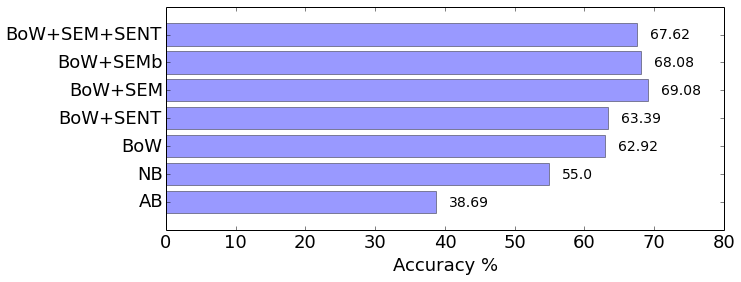
\includegraphics[width=\columnwidth]{ch06_similarity_pics/results2.png}
    \caption{Percentage of accuracy of the different approaches. AB refers to the AcousticBrainz framework. NB refers to the method based on Na\"{i}ve Bayes from \cite{Hu2005}.}
    \label{fig:similarity:results}
\end{figure}

%A comparison of the confusion matrix of the AcousticBrainz audio-based approach and the BoW+Sem text-based approach is shown in Table~\ref{tbl:similarity:confusion}. We observe that, although the text-based approach has higher accuracy in all the categories, both aporaches have a similar behaviour. This can explain why the combination of acoustic features with text-based features does not improve pure text-based approaches. We also note that both approaches have low accuracy values when distinguishing between Classic Rock and Alternative Rock. This means that the difference between these two categories is highly subtle, and neither acoustic nor text-based descriptors are able to properly help the classifier.


\subsection{Results and Discussion}

Accuracy results of the two baseline approaches introduced in Section \ref{sec:similarity:baselines} along with our approach variants are shown in Figure~\ref{fig:similarity:results}. At first sight, we may conclude that sentiment features contribute to slightly outperforming purely text-based approaches. This result implies that affective language present in a music review is not a salient feature for genre classification (at least with the technology we applied), although it certainly helps. On the contrary, semantic features clearly boost pure text-based features, achieving 69.08\% of accuracy. The inclusion of broader categories does not improve the results in the semantic approach. The combination of semantic and sentiment features improves the BoW approach, but the achieved accuracy is slightly lower than using semantic features only.%Although unreported due to space constraints, additional feature combinations were evaluated, considering for instance acoustic features, but their results were in general lower. 
% No creo que haga falta decir "lower than the systems in the figure bla", se sobreentiende no?

%Our aim in this experiment is to measure the impact of semantic and sentiment features in a text-based approach for genre classification. In addition, we want to compare these results with state-of-the-art audio-based approaches. The combination of acoustic and textual features is out of the scope of this chapter.
%The different approaches are built by linear aggregation of the different feature vectors. The approach used for genre classification is trained and tested on a Linear SVM classifier with L2 penalty. The dataset was split for each genre in 80\% for training and 20\% for testing. In addition, we applied 5-fold cross validation and averaged the results. Results of the three baseline approaches plus 3 text-based approaches with different combinations of features and are shown in Figure~\ref{fig:similarity:results}. We observe that sentiment features slightly outperforms a pure text-based approach. This result implies that measuring the positiveness or negativeness in the language used in a music review is not a salient feature for genre classification, although it certainly help. By contrast, semantic features really boost accuracy. The addition of external semantic information related to the entities present in the review help in the process of classification. We tried further combinations of features, including semantic, sentimental and acoustic features, but results did not improve the ones presented in Figure~\ref{fig:similarity:results}.

Let us review the results obtained with baseline systems. The Na\"{i}ve Bayes approach from \cite{Hu2005} is reported to achieve an accuracy of 78\%, while in our results it is below 55\%. The difference in accuracy may be due to the substantial difference in length of the review texts. In \cite{Hu2005}, review texts were at least 3,000 characters long, much larger that ours. Moreover, the addition of a distinction between Classic Rock and Alternative Rock is penalizing our results. 
As for the acoustic-based approach, although the obtained accuracy may seem low, it is in fact a good result for purely audio-based genre classification, given the high number of classes and the absence of artist bias in the dataset \cite{bogdanov2016cross}.
%As for the acoustic-based approach defined in \cite{Tzanetakis2002}, they achieve 61\% accuracy on the GZTAN dataset. However, certain bias in this dataset \cite{Sturm2012} may be responsible of such high performance. Therefore, we have taken the computation done in AcousticBrainz using this approach and trained on the GZTAN dataset to our dataset. As this approach classify a song among 10 different genres, and our dataset have 13 genres, we computed the average accuracy among the results only for this 10 genres. 
Finally, we refer to Table~\ref{tbl:similarity:confusion} to highlight the fact that the text-based approach clearly outperforms the acoustic-based classifier, although in general both show a similar behaviour across genres. Also, note the low accuracy for both Classic Rock and Alternative Rock, which suggests that their difference is subtle enough for making it a hard problem for automatic classification.

%We  did some trials at different character length, and this aspect revealed to be very determinant in the accuracy results. After performing several tests did some trials at different character length, and this aspect revealed to be very determinant in the accuracy results. In addition, the addition of a distinction between Classic and Alternative Rock is penalizing the results, as it has shown to be a difficult task. However, the aim of this experiment is compare different approaches among them, rather than achieving a very high value of accuracy.
%Furthermore, the acoustic-based approach defined in \cite{Tzanetakis2002} presents a result of 61\% of accuracy in the GZTAN dataset. However, some biases in the dataset \cite{Sturm2012} may be responsible of such a high level. Therefore, we have taken the computation done in AcousticBrainz using this approach and trained on the GZTAN dataset to our dataset. As this approach classify a song among 10 different genres, and our dataset have 13 genres, we computed the average accuracy among the results only for this 10 genres.


\begin{table*}[]
\centering
\scriptsize
\begin{tabular}{|l|r|r|r|r|r|r|r|r|r|r|r|r|r|}
\hline
& Alt. Rock & Classical & Country & Electronic & Folk & Jazz & Latin & Metal & New Age & Pop & R\&B & Hip-Hop & Rock  \\
\hline
Alt. Rock & 28 / 42 & 1 / 3 & 3 / 1 & 10 / 10 & 7 / 1 & 1 / 2 & 2 / 0 & 18 / 12 & 10 / 2 & 4 / 10 & 3 / 6 & 3 / 2 & 10 / 9 \\
Classical & 0 / 0 & 87 / 95 & 1 / 0 & 0 / 0 & 1 / 1 & 1 / 1 & 2 / 2 & 1 / 0 & 5 / 1 & 1 / 0 & 0 / 0 & 0 / 0 & 1 / 0 \\
Country & 2 / 1 & 0 / 0 & 51 / 84 & 3 / 0 & 9 / 1 & 9 / 0 & 3 / 0 & 0 / 1 & 3 / 0 & 8 / 8 & 6 / 4 & 1 / 0 & 5 / 1 \\
Electronic & 7 / 3 & 3 / 1 & 1 / 2 & 40 / 61 & 4 / 1 & 1 / 2 & 2 / 2 & 6 / 0 & 7 / 5 & 6 / 5 & 6 / 7 & 13 / 5 & 4 / 7 \\
Folk & 4 / 6 & 11 / 0 & 13 / 10 & 7 / 0 & 27 / 55 & 6 / 1 & 7 / 3 & 4 / 2 & 6 / 9 & 5 / 9 & 6 / 4 & 1 / 0 & 3 / 1 \\
Jazz & 7 / 0 & 10 / 1 & 6 / 2 & 2 / 2 & 5 / 0 & 45 / 82 & 6 / 3 & 3 / 0 & 8 / 2 & 3 / 5 & 4 / 1 & 1 / 1 & 0 / 1 \\
Latin & 4 / 3 & 6 / 4 & 9 / 2 & 1 / 2 & 5 / 1 & 10 / 2 & 28 / 78 & 3 / 0 & 6 / 2 & 11 / 4 & 7 / 2 & 5 / 0 & 5 / 0 \\
Metal & 13 / 5 & 1 / 0 & 1 / 1 & 2 / 2 & 1 / 0 & 0 / 1 & 1 / 0 & 63 / 87 & 1 / 0 & 1 / 0 & 3 / 1 & 1 / 0 & 12 / 3 \\
New Age & 9 / 2 & 7 / 6 & 9 / 0 & 7 / 4 & 10 / 10 & 9 / 2 & 7 / 6 & 3 / 3 & 15 / 53 & 10 / 7 & 6 / 1 & 2 / 1 & 6 / 5 \\
Pop & 6 / 2 & 9 / 1 & 10 / 2 & 9 / 2 & 5 / 3 & 9 / 2 & 5 / 2 & 2 / 0 & 7 / 1 & 19 / 73 & 7 / 6 & 2 / 2 & 10 / 5 \\
R\&B & 8 / 2 & 0 / 1 & 16 / 3 & 8 / 4 & 2 / 0 & 5 / 3 & 5 / 0 & 1 / 0 & 3 / 0 & 7 / 10 & 24 / 71 & 17 / 5 & 4 / 1 \\
Hip-Hop & 8 / 2 & 0 / 0 & 2 / 1 & 8 / 2 & 0 / 1 & 0 / 1 & 1 / 0 & 4 / 3 & 2 / 0 & 4 / 1 & 7 / 2 & 61 / 86 & 3 / 1 \\
Rock & 17 / 15 & 1 / 2 & 6 / 8 & 4 / 7 & 10 / 5 & 2 / 4 & 7 / 1 & 12 / 13 & 4 / 1 & 9 / 7 & 7 / 4 & 6 / 2 & 15 / 31 \\
\hline
\end{tabular}
\caption{Confusion matrix showing results derived from AB acoustic-based classifier/BoW+SEM text-based approach.}
\label{tbl:similarity:confusion}
\end{table*}


\section{Conclusion}
\label{sec:similarity:conclusion}

In this chapter we presented several methodologies that exploit semantic technologies for computing artist similarity and music genre classification. Particularly, we focus on the use of entity linking as a medium to enrich the information present in musical documents. Results in both tasks show that the addition of semantic information via entity linking clearly yields performance improvements.

Different methods to embed this semantic information have been proposed, from knowledge graphs to vector space models.
In the case of artist similarity, the proposed methodology is divided in three main steps: First, named entity mentions are identified in the text and linked to a knowledge base. Then, these entity mentions are used to construct a semantically motivated knowledge representation. Finally a similarity function is defined on top of the knowledge representation to compute the similarity between artists.
For each one of these steps we explored several approaches, and evaluated them against a small dataset of 188 artist biographies, and a larger dataset of 2,336 artists, both obtained from Last.fm.
Results showed that the combination of semantically enriched graphs via entity linking, and a maximal common subgraph similarity measure clearly outperforms a baseline approach that exploits word co--occurrences and latent factors.

In the case of music genre classification, a multimodal dataset of album customer reviews combining text, metadata and acoustic features gathered from Amazon, MB and AB respectively is used. Customer review texts are further enriched with named entity disambiguation along with polarity information derived from aspect-based sentiment analysis. Based on this information, a text-based genre classifier is trained using different combinations of features. 
A comparative evaluation of features suggests that a combination of bag-of-words and semantic information has higher discriminative power, outperforming competing systems in terms of accuracy.

In the light of these results on both tasks, the following conclusions can be drawn: First, semantic approaches may outperform pure text-based approaches. Second, we observe that the inclusion of knowledge leveraged from external ontologies boost the performance on both tasks. Finally, reducing noise by filtering linked entities by type is a rewarding step that contributes to an improved performance.

\cleartorecto%!TEX root = ../thesis_a4.tex

\chapter[Sound and Music Recommendation with Knowledge Graphs][Sound and Music Rec. with KGs]{Sound and Music Recommendation with Knowledge Graphs}
\label{sec:graph-rec}

\section{Introduction}
\label{sec:graph-rec:introduction}

In this chapter we tackle the problem of computing sound and music recommendations following a hybrid approach that leverages semantic content features extracted from textual descriptions and collaborative features from implicit user feedback. 
%Among all registered users there is a low percent of highly engaged users that have been continuously contributing to the site, not only uploading sound, but also commenting, rating and discussing in the forum. 
%All sounds have attached a number of tags and a textual description, which are added by contributors at the time of uploading. 
%Only registered users can download sounds published by other users, but anyone who access the site can search, browse and listen to sounds. 
%A general characterization of its community of users can be found in \cite{Font2012}. 
The approach we propose to recommend musical items consists mainly of two parts: (i) the enrichment of original data attached to items and linkage to knowledge repositories, (ii) the effective exploitation of the graph-based nature of such data for computing the recommendations. 

The enrichment of data consists in using entity linking techniques for extracting semantic entities from item textual descriptions and linking them to external knowledge bases such as WordNet \citep{wordnet} and DBpedia \citep{dbpedia1} for gathering additional knowledge. All those different information are eventually merged together and represented by means of a new knowledge graph (KG), following a similar approach to the one described in Section~\ref{sec:similarity:semantic_enriched_graph}.
This latter graph is thus exploited together with collaborative information from implicit feedback for computing the recommendations. Two graph feature mappings are defined to leverage the new knowledge graph and obtain expressive feature representations. All different features are combined together in a feature combination hybrid schema \citep{Burke2002} and used to feed a content-based recommender. An extensive experimental evaluation was carried out on two different datasets --one related to sounds and other to songs-- to evaluate the recommendation quality in terms of accuracy, novelty and aggregated diversity. 

In this chapter, we deal with two slightly different problems in the music ecosystem. We address the songs recommendation problem and that of recommending sounds to users in online sound sharing platforms. The two tasks addresses two separate categories of users in the music domain: on the one hand, we have music consumers (songs and artists recommendation); on the other hand, we have music producers (sounds recommendation).

Music recommendation has received a lot of attention in the last decade \citep{oscarBook,Knees2013}. As a matter of fact, the discovery of new songs and artists is a task that the music consumers of a Web radio or of a music store are naturally led to perform daily. Hence, helping them by recommending the best choices results in immediate impact also in industrial and commercial scenarios.
%The motivation behind a music recommender system seems to be clear, as music consumers typically want to discover new songs and artists. Thus, the problem of music recommendation has been widely studied in the last decade \citep{knees_schedl2013}. 

Differently from the previous case, recommendation of sounds has received scant attention even though it may be of interest in many scenarios of music creation. As an example, we may consider producers of electronic music that typically downloads and use sound samples. They might be interested in the recommendation of relevant sounds downloaded by users with similar tastes or similar (not equal) to those they previously used in their musical compositions. Likely, they are also looking not just for popular sounds as they want their production to be unique.
To this end, we first centered our study in Freesound\footnote{\url{http://freesound.org}}, one of the most popular sites on the Web for sharing audio clips, accounting more than 6 million registered users and about 350k uploaded sounds, which are described in terms of textual descriptions and tags. In Freesound, different kind of users may be observed \citep{Font2012} (e.g. music producers, composers, sound designers, soundscape enthusiasts), and also different types of sounds (e.g. sound samples, field recordings, soundscapes, loops).
% Hence, recommending sounds is not a trivial task and requieres on the one hand a high level of personalization, and on the other hand, a thoroughly annotation of the items. 
We have the intuition that collaborative features may help in the personalization of the recommendations, whilst the introduction of semantic features may lead to a better exploitation of less popular items. To evaluate this hypothesis, a dataset composed of sound descriptions and historical data about user's download behavior was collected.

To demonstrate the suitability of the proposed methodology for both types of musical users (producers and consumers), a music recommendation experiment was also performed. To this end, a dataset of songs which combines tags and textual descriptions with users' implicit feedback was created by aggregating information gathered from Songfacts\footnote{\url{http://songfacts.com}} and Last.fm\footnote{\url{http://last.fm}}. Songfacts is an online database that collects, stores and provides facts, stories and trivia about songs, whilst in Last.fm a detailed profile of each user's musical taste is built by recording details of the tracks the user listens to.

%We have the intuition that combining collaborative information with implicit semantics extracted from sound descriptions may be useful to achieve this level of personalization.
% talk about why recommendation
%In Freesound, sounds are originally described in terms of textual descriptions and tags which are in turn classified in a tagging ontology.
The evaluation performed on both datasets showed that the semantic expansion of the original data combined with user collaborative features allows the system to enhance recommendation quality especially in terms of aggregated diversity and novelty while keeping high performance in terms of accuracy. %This turn out in a higher level of personalization of recommendations, in terms of prediction accuracy, catalog coverage and long tail recommendations.

%Our main contributions in this chapter are summarized as follows:
%\begin{itemize}
%\item{We define a novel method to enrich the description of musical and sound items with semantic information.}
%\item{We propose two different graph-embedding approaches to encode knowledge graph information into a linear feature representation.}
%\item{We present a methodology to recommend musical items combining semantic and collaborative features, that turns out in a high level of personalization of recommendations, in terms of prediction accuracy, catalog coverage and long tail recommendations.}
%\item{We tackle for the first time the problem of sound recommendation.}
%\end{itemize}

%To confirm the results obtained in the sound recommendation scenario and demonstrate the suitability of the proposed methodology to other types of musical items, a second experiment was performed. For this purpose, a dataset of songs combining tags and textual descriptions with user's implicit feedback was created by aggregating information gathered from Songfacts.com and Last.fm. Songfacts.com is an online database that collects, stores and provides facts, stories and trivia about songs, whilst in Last.fm a detailed profile of each user's musical taste is built by recording details of the tracks the user listens to.
%Results on the second experiment confirm that the addition of semantic features by means of the proposed graph embedding methods, turn out in a higher level of personalization of recommendations, in terms of prediction accuracy, catalog coverage and long tail recommendations.

%\input{src/related_intro}

The reminder of the chapter is structured as follows. The next section introduces the basic technologies used to build the knowledge graph at the basis of our recommendation system. Section \ref{sec:graph-rec:enrichment} describes the problem and the semantic expansion applied to the initial data. Then, Section \ref{sec:graph-rec:approach} defines the adopted recommendation approach while in Section \ref{sec:graph-rec:evaluation} we explain the experimental evaluation and discusses the obtained results. Finally, Section \ref{sec:graph-rec:conclusion} concludes the chapter.


\section{Knowledge enrichment via entity linking}
\label{sec:graph-rec:enrichment}
%An enrichment of our initial knowledge graph was performed by extracting and linking both tags and keywords from textual descriptions to external knowledge bases by means of entity linking techniques.
%A musical item (e.g. an artist, a song, a sound sample) may have context information associated, such as text, tags, photos, etc. This information can be semantically exploited to create a knowledge graph. More specifically, unstructured textual information can be converted into a semantic netchapter of entities by means of an entity linking process. Following this process, unlabeled semantic relations may emerge between the initial music entity and the entity mentions present in its context.
 
In order to add more semantics to the description of musical items, we exploit contextual information, i.e., tags and text descriptions, %to link more entities to the ones already available in Freesound thus enriching 
and then use this information to create a knowledge graph. 
%To represent the new entities we extended the original ontology  by plugging in a new set of classes and related properties (see the green dashed arrows and the green boxes in Fig. \ref{fig:graph-rec:fso_enhancement}). Following the Linked Data principles\footnote{\url{http://www.w3.org/DesignIssues/LinkedData.html}}, we reused classes and properties from external vocabularies. The final ontology after the entity linking and expansion process contains three new classes: \texttt{wordnet:Synset}, \texttt{Entity} and \texttt{skos:Concept} and five new relations: \texttt{wordnet:synset\_member}, \texttt{dcterms:relation}, \texttt{dcterms:subject}, \texttt{skos:broader} and \texttt{wordnet:hypernym}\footnote{All the prefix we use here are the ones available via the \url{http://prefix.cc} service}.
%Several approaches have been developed to enrich folksonomies with semantics. According to \citep{Garcia2012} they may be based on clustering techniques, the usage of ontologies or a combination of them both.
Several approaches have been developed to enrich tags with semantics \citep{Garcia2012}. We follow an ontology-based approach, enriching both tags and keywords extracted from textual descriptions by associating them with relevant entities defined in online knowledge repositories.
The first step in this direction is to link and disambiguate tags and keywords to Linked Data resources. 
For this purpose we adopted Babelfy %, a state of the art tool for Entity Linking and Word Sense Disambiguation 
\citep{Moroetal2014}. We selected this tool as it is able not only to disambiguate named entities, but also concepts. Our intuition here is that the disambiguation of concepts used to describe sounds may be useful to enrich their descriptions. Babelfy output is further enriched with ELVIS (see Section~\ref{sec:linking:elvis}). Thus, for every mapped and disambiguated text fragment, we obtain the related DBpedia, and/or WordNet \textit{synset}. For DBpedia entities we also obtain the associated Wikipedia categories.

%Babelfy maps words from a given text to entities in the BabelNet\footnote{\url{http://babelnet.org}} knowledge base. 
%BabelNet is a multilingual encyclopedic dictionary that mixes knowledge from WordNet and Wikipedia. Thus, for every mapped and disambiguated text fragment, Babelfy returns the related WordNet \textit{synset}, and/or the related Wikipedia page (and its equivalent DBpedia resource).  

To build our semantically enriched graph, the entity linking tool is firstly run on both tags and keywords of every item. Identified named entities are linked to DBpedia resources, whilst disambiguated words are linked to WordNet \textit{synsets}. Every musical item is added to the graph. Then, for each item, text spans from its context identified as entities are added to the graph, and connected to the item. We refer to these text spans as \textit{keywords}. Keywords are in turn connected with their corresponding URIs, whether they are a DBpedia resource or a WordNet \textit{synset}.
Subsequently, we use both WordNet and DBpedia to semantically expand the entities added to the graph after the entity linking phase. 
Each synset obained from the linking is further expanded considering other concepts in the WordNet hierarchy of sysnsets by following the hypernymy\footnote{Hypernymy models generalization relations between synsets.} relations. 
%Once the synset of a word is obtained, the WordNet hierarchy of sysnsets may be explored. 
%In this hierarchy, synsets are connected by two relations: hypernymy and meronymy. The former models generalizations between synsets while the latter represents part-of relations. 
%For the scope of this research we only took into consideration hypernymy relations between synsets. 
From the WordNet hierarchy we extract up to 2-hop hypernyms starting from the mapped synset. We empirically selected the maximum distance of two hops because we wanted to avoid too broad generalization of the original concept. For the same reason we discard those hypernyms farther less than six hops away from the root of the WordNet hierarchy. %The experimental results show (see Section \ref{sem_eval}) that this restriction in the semantic expansion of WordNet concepts does not affect negatively the results of the recommendation engine fed by our knowledge graph. 
% the length of the longest hypernym path from a synset to the root of the WordNet hierarchy should be at least six.
Regarding DBpedia, our entity linking pipeline returns the URI of the linked entity and a set of related Wikipedia categories. In DBpedia, resources are related to categories through the property \texttt{dcterms:subject}. Those categories are in turn organized in a taxonomy. In particular, more specific categories are related to more generic ones by means of the \texttt{skos:broader} property. Thus, for each category retrieved, all the direct broader categories were gathered and added to our knowledge graph. To avoid too broad or unrelated categories, only one level of broader categories were considered.

To show an example of entity linking performed by Babelfy we use the sound \texttt{prac-snare2.wav}\footnote{\url{http://www.freesound.org/people/TicTacShutUp/sounds/439/}} from Freesound. The description associated to this sound is \textit{"standard snare sample. lower/mid tuning on the head"} and tags are \textit{drums}, \textit{percussion}, \textit{snare}. Babelfy was able to detect and link most of the entities. Just to describe a few of them, the word \textit{sample} from the description was linked to the DBpedia entity \texttt{Sampling\_(music)}, the tag \textit{percussion} was mapped to the DBpedia entity \texttt{Rythm\_section}, the tag \textit{snare} was linked to the WordNet concept \texttt{snare\_drum.n.01} and DBpedia entity \texttt{Snare\_drum}. As shown in Figure~\ref{fig:graph-rec:graph_enhancement}, DBpedia entities and WordNet synsets are then further enriched with their related categories and hypernyms. Following the Linked Data principles\footnote{\url{http://www.w3.org/DesignIssues/LinkedData.html}}, we reused classes and properties from external vocabularies. The final knowledge graph after the entity linking and expansion process contains four main classes: \texttt{wordnet:Synset}, \texttt{Entity}, \texttt{Tag} and \texttt{skos:Concept} and seven relations: \texttt{hasTag}, \texttt{hasKeyword}, \texttt{wordnet:synset\_member}, \texttt{dcterms:relation}, \texttt{dcterms:subject}, \texttt{skos:broader} and \texttt{wordnet:hypernym}\footnote{All the prefix we use here are the ones available via the \url{http://prefix.cc} service}.
%In particular, for the sounds recommendation dataset based on Freesound we further enriched the ontology originally developed in \cite{Font2014} as also shown in the left hand side of Figure~\ref{fig:graph-rec:graph_enhancement}. 
% (see Figure~\ref{fig:graph-rec:graph_enhancement}).

%We performed a manual check of many entity linking outputs and observed that sound textual descriptions, even when short, were very informative in most of the cases, and contained relevant keywords that were not explicitly represented in the list of tags. Figure \ref{fig:graph-rec:graph_enhancement} shows a portion of the final knowledge graph.

\begin{figure*}
\centering
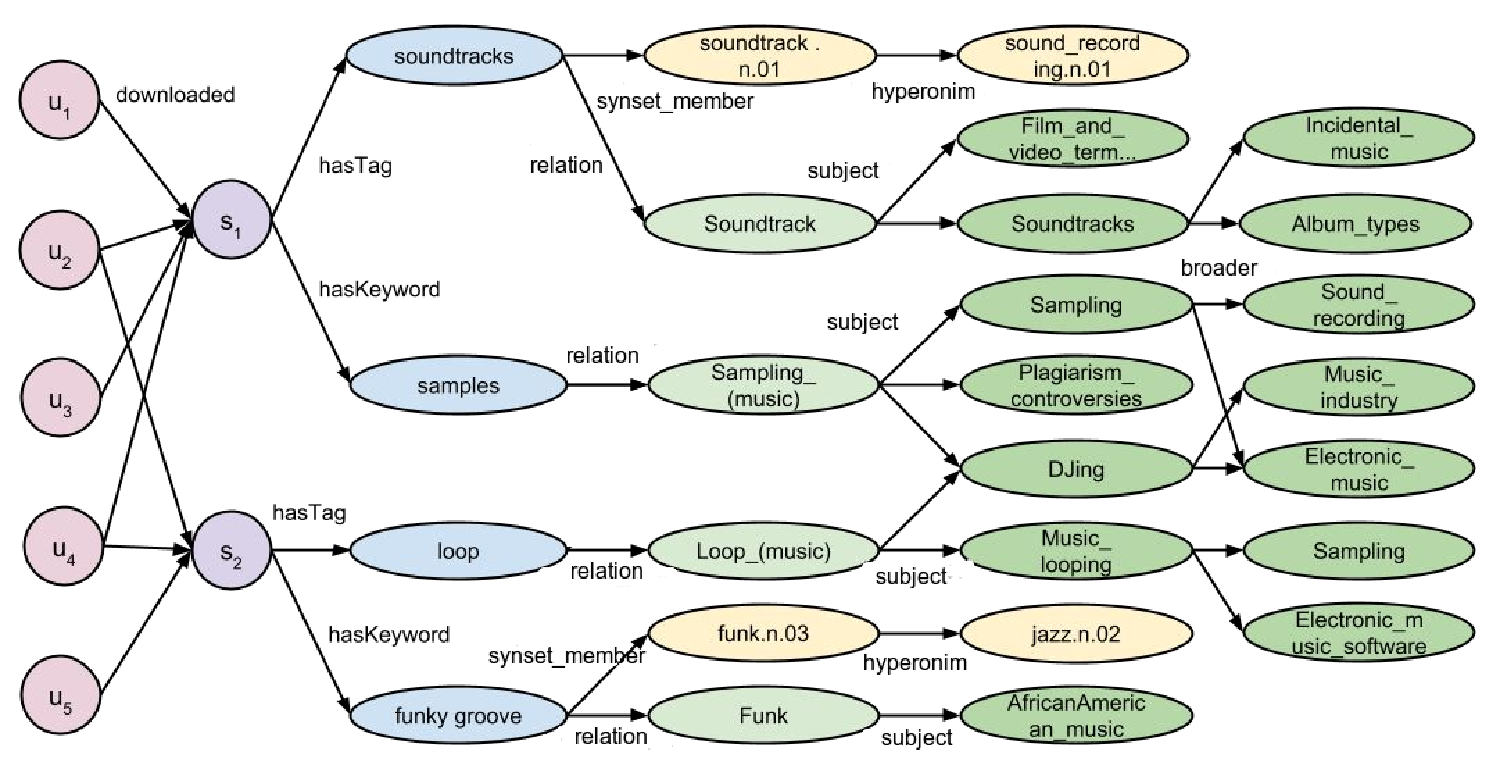
\includegraphics[width=\textwidth]{ch07_graph-rec_pics/graph_all_final2.pdf}
\caption{Portion of the final knowledge graph enriched with WordNet and DBpedia \label{fig:graph-rec:graph_enhancement}}
\end{figure*}


\section{Recommendation approach}
\label{sec:graph-rec:approach}
As aforementioned, we adopted a hybrid recommendation approach to leverage both collaborative information coming from the user's community and content information coming from the knowledge graph. 
Following the taxonomy of hybrid recommender systems presented in \cite{Burke2002} we developed a hybrid feature combination recommender system. 
The particularity of such schema is that hybridization is not based on the combination of different recommendation components but instead on the combination of different data sources. 
Specifically, collaborative information is treated as additional features of the content feature space and a content-based technique is used over this augmented space. Therefore, we build feature item representations by considering the item graph-based descriptions represented in the knowledge graph and enrich such feature vectors with collaborative features. Subsequently, we use such data to feed a content-based recommendation engine. 

A common way of computing content-based recommendation is learning a function that, for each item in the system, predicts the relevance of such item for the user. 
The application of Machine Learning techniques is a typical way to accomplish such task. % \cite{pazzani}. 
A \textit{top-N}\xspace item recommendation problem in a standard content-based setting is mainly split into two different tasks: 
(i) given a collection of items for which past user's preferences are available, learn a regression or classification model to predict the relevance associated to unknown items; (ii) eventually, according to such scores, recommend the most relevant items to the user. 
Past user's preferences can be obtained from either explicit or implicit feedback. As for Freesound, we considered as an implicit positive feedback the ``download data''. The rationale behind our choice is that if a user downloads a sound it is reasonable to assume that she likes it even without an explicit rating, as the system lets users listen to sounds before downloading. Also the Last.fm dataset used in the experimental evaluation contains user song listening actions, which is another form of implicit feedback. 
Thus, in the following we will refer to the problem of computing recommendations from implicit feedback data. 
Following the notation introduced by \cite{RendleFGS09} for implicit feedback scenarios, let $S$  be the matrix of implicit feedback, where $s_{ui}=1$ if item $i$ was downloaded from user $u$, 0 otherwise. 
Starting from $S$ we define $I_u^+ = \lbrace i \in I |  s_{ui}=1\rbrace$ as the set of relevant items for $u$. 
The main problem with implicit feedback is that they reflect only positive user preferences. On the contrary, the system cannot infer anything about what the user dislikes. The unobserved data are a mixture of actually negative and missing values \citep{RendleFGS09}, but the system does not have any information for discriminating between them. 
Then, learning a predictive model from such unary data becomes infeasible because there are no negative examples. To overcome this issue for each user we select a portion of unobserved items $I_u^- \subset (I \setminus I_u^+)$ to be used as negative data points in the training of the model. In \cite{Ostuni2013}, the authors show that choosing $|I_u^-| = 2\cdot |I_u^+|$ does not affect accuracy results.
The unobserved items are exactly the items that have to be ranked. The ultimate goal of the system is to rank in the \textit{top-N}\xspace positions items likely to be relevant for the user. 

Given the generic user $u$, let $T_u$ be the training set for $u$ defined as:
\[
T_u=\lbrace \langle x_i,s_{ui} \rangle |  i \in (I_u^+ \cup I_u^-)\rbrace
\] 
where $x_i \in \mathbb{R}^D$ is the feature vector associated to the item $i$ and let $TS_u$ be the test set defined as:
\[
TS_u=\lbrace \langle x_i,s_{ui}^* \rangle |  i \in (I \setminus I_u^+)\rbrace
\]
The two tasks for the \textit{top-N}\xspace recommendation problem, in our setting, consist then of: (i) learning a function $f_u:\mathbb{R}^D \rightarrow \mathbb{R}$ from the training data $T_u$  which assigns a relevance score to the items in $I$; (ii) using such function to predict the unknown score $s_{ui}^*$ in the test set $TS_u$, to rank them and recommend the \textit{top-N}\xspace.
%\begin{enumerate}
%\item learning a function $f_u:\mathbb{R}^D \rightarrow \mathbb{R}$ from the training data $T_u$  which assigns a relevance score to the items in $I$;
%\item using such function to predict the unknown score $s_{ui}^*$ in the test set $TS_u$, rank them and recommend the \textit{top-N}\xspace.
%\end{enumerate}

Given that items are represented as entities in a knowledge graph we are particularly interested in those machine learning methods that are appropriate for dealing with objects structured as graphs. 
There are two main ways of learning with structured objects. The first is to use \textit{Kernel Methods} \citep{Cristianini}. 
Given two input objects $i$ and $j$, defined in an input domain space $D$, the basic idea behind Kernel Methods is to construct a kernel function $k: D \times D \rightarrow \mathbb{R}$, that can be informally seen as a similarity measure between $i$ and $j$. This function must satisfy $k(i,j) = \langle \phi(i),\phi(j) \rangle$ for all $i,j \in D$, where $\phi :D \rightarrow F$ is a mapping function to a inner product feature space $F$. 
Then, the classification or regression task involves linear convex methods based exclusively on inner products computed using the kernel in the embedding feature space. 
The alternative way is to explicitly compute the \textit{explicit feature mapping} $\phi(i)$ and to directly use linear methods in the related space. 
By transforming the graph domain into a vector domain any traditional learning algorithm working on feature vectors can be applied. 

While kernel methods have been widely applied to solve different tasks, their usage becomes prohibitive when dealing with large datasets. 
%because of their scalability bottleneck. % \cite{Pham2013}. 
In addition, when the input data lie in a high-dimensional space, linear kernels have performances comparable to more complex non linear ones. 
Due to the high volume of users we deal with in our Freesound dataset (see Section \ref{sec:graph-rec:evaluation}), we focused on learning methods which are computationally efficient. For this reason we adopted the approach of computing the explicit feature mapping of the item graphs and use linear methods to learn the user model. Specifically, we use the Linear Support Vector Regression \citep{HoL12} algorithm. 
Regarding the explicit feature mapping computation we define two sparse high-dimensional feature maps: the one based on entities, the other on paths that we call \textit{entity-based item neighborhood mapping} and \textit{path-based item neighborhood mapping}, respectively. In the following we formalize the computation of such graph embeddings.

\subsection{Explicit feature mappings for graph-based item representations}
%Let us formally define the knowledge graph as a multi-relational graph $G=\lbrace t \mid t \in E \times R \times E \rbrace$, where $E$ denotes the set of entities and $R$ indicates the set of properties or relations, namely the edge labels. Moreover, we have $I \subseteq E$ since we consider items as a particular type of entities.\\
%With $E^h_i$ we denote the set of entities reachable in \textit{at most h} hops from $i$ according to the shortest path in $G$. For a generic item $i$ we then define its h-hop neighborhood graph $G^h_i=\lbrace t=(e_i,r_j,e_k) \mid t \in E^h_i \times R \times E^h_i \rbrace$ that is the subgraph of $G$ induced by the set of triples involving entities in $E^h_i$. 

Following the formal definition of a multi-relational knowledge graph $G=\lbrace t \mid t \in E \times R \times E \rbrace$ and an h-hop item neighborhood graph $G^h_i=\lbrace t=(e_i,r_j,e_k) \mid t \in E^h_i \times R \times E^h_i \rbrace$ stated in Section~\ref{sec:similarity:method:sim:mcs}, Figure \ref{fig:graph-rec:Example} shows an example of 2-hop item neighborhood graph for item $i$, namely $G^2_i$. We see that, if we consider the shortest path, all the entities are no more than 2 hops distant from $i$. 

\begin{figure}
\begin{center}
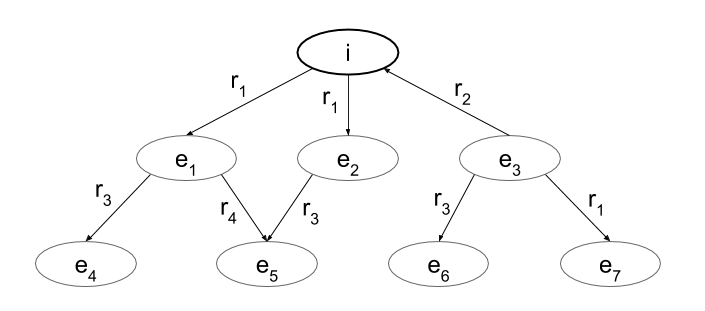
\includegraphics[width=0.8\textwidth]{ch07_graph-rec_pics/item_neig2.png}
\end{center}
\caption{An example of 3-hop item neighborhood graph for the item $i$.}
\label{fig:graph-rec:Example}
\end{figure}

To clarify the definition and computation of $G^h_i$ and $E^h_i$ for item $i$, we show their computation with reference to the example shown in Figure \ref{fig:graph-rec:Example}:\\ 
$G^1_i= \lbrace (i,r_1,e_1), (i,r_1,e_2), (e_3,r_2,i)\rbrace$\\ 
$G^2_i= G^1_i \bigcup \lbrace (e_1,r_3,e_4), (e_1,r_3,e_5), (e_2,r_4,e_5), (e_3,r_6,e_6),(e_3,r_1,e_7) \rbrace$\\
$E^1_i= \lbrace e_1, e_2, e_3 \rbrace$\\
$E^2_i=  E^1_i \bigcup  \lbrace e_4, e_5, e_6, e_7 \rbrace$\\

Starting from those item graph-based representations we define the two different feature mappings which are described in what follows.

\subsubsection{Entity-based item neighborhood mapping}

In this mapping each feature refers to an entity in $E$ and the corresponding score represents the weight associated to that entity in $G^h_i$. The resulting feature vector $\phi_E(G^h_i)$ is:
\[
\phi_E(G^h_i)=(w_{i,e_1} ,w_{i,e_2} ,...w_{i,e_m} ,...,w_{i,e_t} )
\]
where the weight associated to the generic entity $e_m$ is computed as follows:

\[
w_{i,e_m}=\sum \limits_{l=1}^{h} {\alpha_l \cdot c_{l,e_m}}
\] 
with 
\[
\alpha_l =\frac{1}{1+\log(l)}
\]
and
%\[
%c_{l,e_m} = \vert \lbrace  (e_n,p,e_m) \textit{  } | \textit{  } e_n \in \widehat{E}^{l-1}_i \textit{ } \vee \textit{ } e_m \in \widehat{E}^l_i \rbrace  \bigcup \]\\
%\[ \lbrace  (e_m,p,e_n) \textit{  } | \textit{  } e_m \in \widehat{E}^l_i  \textit{ } \vee \textit{ }  e_n \in \widehat{E}^{l-1}_i \rbrace \vert
%\]
\begin{multline}
c_{l,e_m} = \vert \lbrace  (e_n,r,e_m) \textit{  } | \textit{  } e_n \in \widehat{E}^{l-1}_i \textit{ } \wedge \textit{ } e_m \in \widehat{E}^l_i \rbrace 
 \bigcup \\ \lbrace  (e_m,r,e_n) \textit{  } | \textit{  } e_m \in \widehat{E}^l_i  \textit{ } \wedge \textit{ }  e_n \in \widehat{E}^{l-1}_i \rbrace \vert \nonumber
\end{multline}
where $ \widehat{E}^l_i =  E^l_i \setminus E^{l-1}_i$ is the set of entities \textit{exactly l} hops far from $i$. 
\\In particular, $c_{l,e_m}$ corresponds to the number of triples connecting $e_m$ to entities in the previous hop \textit{$(l-1)$}, whether $e_m$ appears either as subject or object of the triple. In other words, $c_{l,e_m}$ can be seen as the \textit{occurrence} of the entity $e_m$ in the item neighborhood at distance $l$. 
The more the entity $e_m$ is connected to neighboring entities of $i$, the more it is descriptive of $i$. 
$\alpha_l$ can be seen as a decay factor depending on the distance $l$ from the item $i$, whose aim is to incrementally penalize farther entities from the item. It allows us to take into account the \textit{locality} of those entities in the graph neighborhood. The closer an entity $e_m$ to the item $i$, the stronger its relatedness to it. We use a logarithmic decay. 
%Indeed, the discount factor can also be parametrized defining a specific weight for each hop. In such case, an optimal combination of weights can be found.

With reference to example showed in Figure \ref{fig:graph-rec:Example}, the $c_{l,e_m}$ values are computed as follows: 
$c_{1,e_1} =1$, $c_{1,e_2} =1$, $c_{1,e_3} = 1$, $c_{2,e_4} = 1$, $c_{2,e_5} =2$, $c_{2,e_6} =1$, $c_{2,e_7} =1$.%, $c_{2,e_8} =1$, $c_{3,e_9} =2$, $c_{3,e_{10}} =2$, $c_{3,e_{11}} =1$. All the others are zero.
%The presented graph embedding is an adaptation of the one presented in \cite{ODMD14a}, in this chapter we use a logarithmic discount factor instead of a parametric one.  

%In this mapping each feature refers to an entity in $E$ and the corresponding score represents the weight associated to that entity in $G^h_i$. The resulting feature vector $\phi_E(G^h_i)$ is:
%%\begin{small}
%\[
%\phi_E(G^h_i)=(w_{i,e_1} ,w_{i,e_2} ,...w_{i,e_m} ,...,w_{i,e_t} )
%\]
%where the weight associated to the generic entity $e_m$ is computed as follows:
%\[
%w_{i,e_m}=\sum \limits_{l=1}^{h} { \frac{ c_{l,e_m}}{1+\log(l)}} 
%\] 
%with 
%\[
%c_{l,e_m} = \vert \lbrace  (e_n,p,e_m) \textit{  } | \textit{  } e_n \in \widehat{E}^l_i \vee e_m \in \widehat{E}^l_i \rbrace \vert
%\]
%%\end{small}
%where $ \widehat{E}^l_i =  E^l_i \setminus E^{l-1}_i$ is the set of entities \textit{exactly l} hops far from $i$. 
%In particular, $c_{l,e_m}$ corresponds to the number of triples involving $e_m$, that is the \textit{occurrence} of the entity $e_m$ in the item neighborhood at distance $l$. The more the entity $e_m$ appears in paths originated by $i$, the more it is descriptive of $i$. The denominator can be seen as a decay factor depending on the distance $l$ from the item $i$, whose aim is to incrementally penalize entities farther from the item. It allows us to take into account the \textit{locality} of those entities in the graph neighborhood. The closer an entity $e_m$ to the item $i$, the stronger its relatedness to it. The presented mapping is an adaptation of the one presented in \cite{ODMD14a}.

\subsubsection{Path-based item neighborhood mapping}

Differently from the previous case, in this mapping we represent a feature as a sequence of nodes in $G$. Given two entities $e_1$ and $e_n$, we consider the sequence of nodes $e_1 \cdot e_2 \cdot \ldots \cdot e_{n-1} \cdot e_n$ met while traversing the graph to go from $e_1$ to $e_n$ and we refer to such sequence as \textit{path}. In this  mapping, a feature is then represented by a path. In particular, in this mapping each feature refers to several variants of paths rooted in the item node. 
We first collect all the paths rooted in $i$ which can be indicated as sequence of entities $i\cdot e_1 \cdot e_2 \cdot \ldots \cdot e_{n-1} \cdot e_n$. 
Then, starting from those paths we define various features considering sub-paths of the original paths. Specifically we form sub-paths composed by only those entities progressively farther from the item.
Considering the path given above we build the following features: $e_1 \cdot e_2 \cdot  \ldots \cdot  e_{n-1} \cdot  e_n$, $e_2 \cdot  \ldots \cdot  e_{n-1} \cdot  e_n$, ..., $e_{n-1} \cdot  e_n$, $e_n$. 
The rationale behind this choice is that it allows to explicitly represent substructures shared between items with no overlapping in their immediate neighborhoods but somehow connected at further distance. Items connected to the same entities have same common structures because both closer and further entities are shared. Items connected to different entities which are however linked directly or at a farther distance to same entities  share less or none sub-paths depending on how much far the common entities are, if any.

More formally, let $P_i$ be the set of paths rooted in $i$ and $P^*_i$ be the list of all possible sub-paths extracted from them. We use $p_m(i)$ and $p^*_m(i)$ to refer to the $m-th$ elements in $P_i$ and $P^*_i$, respectively. Then, the feature mapping for item $i$ is:
\[
\phi_P(G^h_i)=(w_{i,p^*_1} ,w_{i,p^*_2} ,...w_{i,p^*_m} ,...,w_{i,p^*_t} )
\]
% paths making up part of larger paths. 
where each $w_{i,p^*_m}$% is the frequency of the feature $p_m$ in $G^h(i)$.  
is computed as:
\[
w_{i,p^*_m}=  \frac{ \# p^*_m(i) }{ \vert p_m \vert - \vert p^*_m \vert} 
\] 
where $\vert p_m \vert$ indicates the length of path $p_m$ and $\# p^*_m(i)$ the occurrence of $p^*_m(i)$ in $P^*_i$. The denominator is a discounting factor which takes into account the difference between the original path $p_m$ and its sub-path $p^*_m$. The shorter the sub-path the more the discount because it contains entities farther from the item. 
\\With respect to item $i$ we have:\\
$P_i= \lbrace i \cdot e_1 \cdot e_4,\text{ }i \cdot e_1 \cdot e_5,\text{ } i \cdot e_2 \cdot e_5,\text{ } i \cdot e_3 \cdot e_6,\text{ } i \cdot e_3 \cdot e_7 \rbrace$\\
$P^*_i= [ e_1 \cdot e_4,\text{ } e_4,\text{ } e_1 \cdot e_5,\text{ }e_5,\text{ } e_3 \cdot e_6,\text{ } e_6
,\text{ } e_3 \cdot e_7,\text{ } e_7 ]$

%Differently from the previous mapping, in this mapping features are represented as a sequences of nodes in $G$. Given two entities $e_1$ and $e_n$, we consider the sequence of nodes $e_1 \cdot e_2 \cdot \ldots \cdot e_{n-1} \cdot e_n$ met while traversing the graph to go from $e_1$ to $e_n$ and we refer to such sequence as \textit{path}. In this  mapping, a feature is then represented by a path. In particular, in this mapping each feature refers to several variants of paths rooted in the item node.
%We first collect all the paths rooted in $i$ which can be indicated as sequence of entities $i\cdot e_1 \cdot e_2 \cdot \ldots \cdot e_{n-1} \cdot e_n$. 
%Then, starting from those paths we define various features considering sub-paths of the original paths. Specifically we form sub-paths composed by only those entities progressively farther from the item.
%Considering the path given above we build the following $n$ features: $e_1 \cdot e_2 \cdot  \ldots \cdot  e_{n-1} \cdot  e_n$, $e_2 \cdot  \ldots \cdot  e_{n-1} \cdot  e_n$, ..., $e_{n-1} \cdot  e_n$, $e_n$. 
%The rationale behind this choice is that it allows to explicitly represent substructures shared between items with no overlapping in their immediate neighboorhoods but somehow connected at further distance. Items connected to the same entities have same common structures because both closer and further entities are shared. Items connected to different entities which are however linked directly or at a farther distance to same entities  share less or none sub-paths depending on how much far the common entities are, if any.
%
%More formally, let $P_i$ be the set of paths rooted in $i$ and $P^*_i$ all possible sub-paths extracted from them. We use $p_m(i)$ and $p^*_m(i)$ to refer to the $m$-th elements in $P_i$ and $P^*_i$, respectively. Then, the feature mapping for item $i$ is:
%\[
%\phi_P(G^h_i)=(w_{i,p^*_1} ,w_{i,p^*_2} ,...w_{i,p^*_m} ,...,w_{i,p^*_t} )
%\]
%% paths making up part of larger paths. 
%where each $w_{i,p^*_m}$% is the frequency of the feature $p_m$ in $G^h(i)$.  
%is computed as:
%\[
%w_{i,p^*_m}=  \frac{ \# p^*_m(i) }{ \vert p_m \vert - \vert p^*_m \vert} 
%\] 
%Here $\vert p_m \vert$ indicates the length of path $p_m$ and $\# p^*_m(i)$ the occurrence of $p^*_m(i)$ in $P^*_i$. The denominator is a discounting factor which takes into account the difference between the original path $p_m$ and its sub-path $p^*_m$. The shorter the sub-path the more the discount because it contains entities farther from the item. 

\subsection{Feature combination}
Each final feature vector $x_i$ is obtained by concatenating a vector of collaborative features $\phi_{col}(i)$ to the item neighborhood mapping vector $\phi(G^h_i)$. Collaborative features are simply added by encoding in the feature vector those users who downloaded that item. The collaborative feature vector regarding the generic item is then:
\[
\phi_{col}(i)=(w_{i,u_1}, w_{i,u_2},...,w_{i,u_1})
\]
where $w_{i,u_1}=1$ if user $u_1$ downloaded item $i$.

Although more sophisticated and advanced methods can be used for feature combination \citep{Beliakov2015}, our experimental evaluation (see Section \ref{sec:graph-rec:evaluation}) shows the effectiveness of our choice.   
%\subsection{Audio-based approach}
%For evaluation purposes, we created a recommendation approach based only on audio content features. Apart from text descriptions and tags, Freesound provides information about acoustic features of the sound signal. Every sound in Freesound is analyzed at the time of the upload using Essentia~\citep{Bogdanov2013}, a library for audio analysis. Moreover, a distance measure between sounds is provided and sounds can be retrieved according to this measure. To calculate the distance between sounds, Personal Component Analysis (PCA) is applied over 352 low-level audio descriptors, reducing the space to 100 dimensions. Then, the euclidean distance between sounds is calculated over the reduced space. 
%
%We define the similarity between two sounds $s_1$, $s_2$ as $sim(s_1,s_2)=1-dist(s_1,s_2)$, being $dist(s_1,s_2)$ the normalized value of the euclidean distance. Based on this measure, we created a simple content-based recommender system. For every user, we ranked all sounds $s_i \in TS_u$ by computing the formula 
%\[
%Score(u,s_i) = \frac{\sum \limits_{ j\in I_u^+}{sim(s_i,s_j)}}{|I_u^+|}
%\]




\section{Experimental evaluation}
\label{sec:graph-rec:evaluation}
For the evaluation of our approach we adopted the \texttt{All Unrated Items} methodology presented in \cite{Steck13}. It consists in creating a \textit{top-N}\xspace recommendation list for each user by predicting a score for every item not rated by that particular user, whether the item appears in the user test set or not. Then, performance metrics are computed comparing recommendation lists with test data.  
The evaluation has been carried out using the holdout method consisting in splitting the data in two disjoint sets: the one for training and the other for testing. We used 80\% of user downloads for building the training set $T$ and remaining 20\% as test data for measuring recommendation accuracy. We repeated the procedure three times by randomly drawing new training/test sets in each round and averaged the results.
%The tuning of model hyper-parameters of the learning algorithm was performed through cross-validation on validation data obtained by selecting the 15\% of feedback for each user from the training data. Specifically we adopted the \textit{LIBLINEAR\footnote{\url{http://www.csie.ntu.edu.tw/~cjlin/liblinear/}}} library. We used the \textit{L2-regularized Support Vector Regression} \cite{HoL12} method and chose the $C$ and $e$ parameters via cross-validation using a grid-search varying $C$ from 0.1 to 1000 with step 10 and $e=\lbrace 0.1,0.01 \rbrace$ (tolerance of termination criterion). Before the training we performed some pre-processing on the feature vectors. We removed those features appearing in less then 5  sounds and scaled all features to the range $[0-1]$ using min-max normalization. Finally each feature vector was normalized to unit length using the L2 norm.

%\subsection{Evaluation Metrics}
For measuring recommendation accuracy we adopted the following standard performance metrics: Precision and Recall. 
Precision@N (P@N) is computed as the fraction of \textit{top-N}\xspace recommended items appearing in the test set, while Recall@N (R@N) is computed as the ratio of \textit{top-N}\xspace recommended items appearing in the test set to the number of items in the test set. Note that in such implicit feedback setting all items in the test set are relevant. In addition to the standard precision and recall metrics we also measure the Mean Reciprocal Rank (MRR) which measure the quality of the highest ranked recommendations. For each user recommendation list the Reciprocal Rank (RR) measures how early in the list is positioned the first relevant recommendation. 

As pointed out by \cite{McNee2006}, the most accurate recommendations according to the standard metrics are sometimes not the recommendations that are most useful to users. In order to assess the utility of a recommender system, it is extremely important to evaluate also its capacity to suggest items that users would not readily discover for themselves, that is its ability to generate novel and unexpected results.
The \textit{Entropy-Based Novelty} (\textit{EBN}) \citep{Bellogin2010} expresses the ability of a recommender system to suggest less popular items, i.e. items not known by a wide number of users. 
In particular, for each user's recommendation list $L_u$, the novelty is computed as:  
\[ EBN_u@N = - \sum \limits_{ i\in L_u} p_i \cdot \log_{2} p_i \]
where:
\[    p_i = \frac{ \vert \lbrace s_{ui}=1 \vert u \in U \rbrace \vert}{  \vert  U  \vert } \]
\noindent Particularly, $p_i$ is the ratio of users who downloaded item \textit{i}. The lower $EBN_u@N$, the better the novelty.

Another important quality of the system is aggregate diversity. 
%its level of personalization which can be measured looking at the aggregate diversity of recommendations across all users. 
In our chapter we adopt the \textit{diversity-in-top-N} metric presented in \cite{adomavicius2012improving} that measures the distinct items recommended across all users. In particular we compute its normalized version with respect to the size of the item catalog. For brevity we refer to it as $ADiv@N$ and we compute it as follows:
\[ ADiv@N = \frac{ \vert \bigcup_u L_u \vert }{ \vert I \vert }  \]
This metric is an indicator of the level of personalization provided by a recommender system. Low values of aggregated diversity indicate  that all users are being recommended almost the same few items. This corresponds to a low level of personalization of the system. Instead, high values mean that users receive very different recommendations which can be indirectly seen as a high level of personalization of the system. %The importance of such particular dimension of the recommendation quality has been also highlighted in other chapters as in \cite{JannachLGB13}.

All the reported metrics, besides aggregated diversity, are computed for each single user and eventually averaged.

\subsection{Datasets description}
\label{sec:graph-rec:datasets}

\subsubsection{Freesound dataset}\label{fs_dataset}
We evaluated our approach on historical data about sound downloads collected from February 2005 to October 2013. In addition, we further enriched our knowledge graphs (see Section~\ref{sec:graph-rec:enrichment}) with information coming from the Freesound Ontology \citep[chapter 6]{font2015tag}, a lightweight ontology where the 500 most popular Freesound tags are classified into 23 tag categories. From the original data dump, we selected a subset of sounds that fulfilled some criteria. We selected those sound with at least two tags classified in the Freesound Ontology. After that we filtered out all sounds with less than 10 downloads to reduce the sparsity of the implicit feedback matrix and have a fairer comparison with pure collaborative filtering methods. 
%After this initial filtering, a total number of 99,008 sounds were obtained out of which 22,000 were randomly selected. Among them, we selected those with at least one entity detected in textual description and linked to WordNet or DBpedia and finally obtained 21,552 sounds. 
%The number of registered users that had downloaded at least 50 of these sounds was 112,723 out of which 20,000 were randomly selected. 
After some further data cleansing, the final dataset consisted in 20,000 users, 21,552 items and 2,117,698 downloads.%\footnote{A dump of the datasets is available at \url{http://mtg.upf.edu/download/datasets/knowledge-graph-rec}}. 
The sparsity of the implicit feedback matrix was 99.51\%. Statistics on the enriched knowledge graph of the final dataset are shown in Table~\ref{tbl:graph-rec:datasets}.

%The total number of different tags found in the final set of sounds was 15,096. From this tag space, 8,160 were mapped to WordNet concepts, 7,099 to DBpedia entities, and 387 were classified in the Freesound Ontology. The average number of mapped tags per item was 6.44. From the textual descriptions, a total number of 23,481 keywords were mapped to 16,706 WordNet synsets, and 16,854 DBpedia entities. The average number of mapped keywords per item was 11.36.
%{\color{red}The full dataset, including hypernyms and broader categories, contains 16,407 DBpedia entities, 54,419 Wikipedia categories, and 20,034 WordNet synsets.}
%In the whole dataset, the number of different DBpedia entities mapped to words was 16,407, and those entities were related to 35,706 different categories. Taking into account also categories connected via the \texttt{skos:broader} property, the total number of categories in the dataset was 54,419. The number of different Wordnet synsets mapped to words was 17,926, and the total number of synsets in the dataset including hypernyms was 20,034.

\begin{table}
\scriptsize
	%[!htb]
	%\tbl{Datasets Overview\label{tbl:graph-rec:datasets}}{%
%	\scriptsize
	\label{tbl:graph-rec:datasets}
	\begin{tabular}{l c c c c c c}
		\toprule
		\textbf{dataset} & \textbf{items} & \textbf{avg. tags} & \textbf{avg. keywords} & \textbf{resources} & \textbf{synsets} & \textbf{categories}\\
		\midrule
		Freesound & 21,552 & 6.44 & 11.36 & 16,407 & 20,034 & 54,419 \\
		Last.fm & 8,640 & 42.09 & 77.33 & 46,109 & 27,708 & 96,942 \\
		\bottomrule
		
	\end{tabular}
	\caption[Number of tags and keywords.]{Number of tags and keywords identified by Babelfy averaged by item, plus total number of distinct DBpedia resources, WordNet synsets and Wikipedia categories.
	}
\end{table}


\subsubsection{Last.fm dataset}\label{fs_dataset}
To recreate most of the conditions of the Freesound dataset in a music recommendation scenario, a new dataset is created combining user's implicit feedback, tags and textual descriptions of songs. This dataset combines a corpus of user's listening habits \citep{Vigliensoni2014}, with tags and textual descriptions about songs. For every user in the corpus we chose the users' average listening count as a threshold to identify the relevant songs for each user. We only selected for our implicit feedback dataset user-song relations with a number of listens above each user's threshold. Moreover, only those songs that were relevant to at least 10 users, and users with at least 50 relevant songs were added to the dataset. The final dataset consisted in 5,199 users, 8,640 songs and 751,531 relations between users and songs. The sparsity of the implicit feedback matrix was 98.33\%.
This collaborative information was complemented with the list of top tags of every song provided by the Last.fm API, and a textual description of each song coming from Songfacts.com (cf. Section~\ref{sec:kb:exp:dataset}). Information about the enriched knowledge graph is shown in Table~\ref{tbl:graph-rec:datasets}.
%We applied the same semantic enrichment process described in Section~\ref{sec:enrichment} to tags and text descriptions. A total number of 38,796 DBpedia entities, 88,556 Wikipedia categories and 15,995 WordNet synsets were added to the Knowledge Graph. The average number of mapped keywords per item was 99.6.


\subsection{Experiment settings}
As mentioned in Section \ref{sec:graph-rec:approach}, each user model is learnt using the Linear Support Vector Regression method. In particular we adopted the efficient \textit{LIBLINEAR\footnote{\url{http://www.csie.ntu.edu.tw/~cjlin/liblinear/}}} library and chose the \textit{L2-regularized Support Vector Regression} \citep{HoL12}. 
The tuning of the model hyper-parameters of the learning algorithm was performed through cross-validation on validation data obtained by selecting the 15\% of feedback for each user from the training data. We set the parameters $C$ and $e$ by using a grid-search varying $C$ from 0.1 to 1000 with step 10 and $e=\lbrace 0.1,0.01 \rbrace$ (tolerance of termination criterion). Before the training we performed some pre-processing on the feature vectors. We removed those features appearing in less than 5 items and scaled all features to the range $[0,\ldots,1]$ using min-max normalization. Finally each feature vector was normalized to unit length using the L2 norm.

%Regarding the run time performances of the entire recommender for the Freesound experiment, the highest computation time (corresponding to the path-based feature mapping with 3-hops) lasted about 28 minutes, from feature extraction to recommendation generation, on a dedicated server machine with 4 Xeon quad-core 2.93GHz processors and 32GB RAM. 
%Since each user model is learnt independently, the learning process is highly parallelizable.  Moreover, being a model-based recommender, each user model learning can be performed offline periodically once a certain number of new feedbacks are accumulated for that specific user. 
%The implementation of the recommendation algorithm presented in this chapter is available on GitHub \footnote{\url{https://github.com/sisinflab/lodreclib}}.

In the following we describe the experiments we carried out to evaluate our approach. In particular we are interested in evaluating the impact of semantic enrichment of the original data on the recommendation quality and the differences among the two feature mapping methods we implemented. Furthermore, we compare our approach with state of the art algorithms for implicit feedback scenarios. 
All the differences between approaches and with respect to other baselines are statistically significant ($p<0.01$) according to the paired t-test.


%%%%%%%%%%%%%%%%%%%%%%%%%%%%%%%%%%%%%%%%%%%%%%%%%%%%%%%%%%%%%%%%%%%%%%%%%%%%%%%%%%%%
\begin{table}
\scriptsize
	%[!htb]
	%\tbl{Freesound Results\label{tbl:graph-rec:Res1}}{%
%	\scriptsize
	\label{tbl:graph-rec:Res1}
\begin{tabular}{l l c c c c c c }
		\toprule
		\textbf{Approach} & \textbf{Enrichment} & \textbf{h-hops} & \textbf{MRR} &  \textbf{P@10} & \textbf{R@10} & \textbf{EBN@10}  & \textbf{ADiv@10}\\
		\midrule
		Ent & fso & h=3 & 0.303 & 0.113  &  0.065 & 2.791	& 0.257   \\
		Ent & fso+KB/tag & h=3 & 0.303 & 0.115  &  0.066  & 2.617 &	0.332  \\
		Ent & fso+KB/tag & h=4 & 0.302 & 0.114  & 0.065  & 2.507 & 0.368  \\
		Ent & fso+KB/kw+tag & h=3 & \textbf{0.306 }& \textbf{0.118}  &  \textbf{0.067}  & 2.426 &	0.361  \\
		Ent & fso+KB/kw+tag & h=4 & \textbf{0.306}  & 0.117 & 0.066  &2.303  & 0.391   \\ 
		Path & fso & h=3 &  0.301 &  0.113  &  0.065   & 2.750 & 0.287   \\
		Path & fso+KB/tag & h=3 & 0.301 &  0.114 &  0.064 & 2.279 	& 0.461   \\
		Path & fso+KB/tag & h=4 &   0.292 & 0.106 & 0.059   & 1.863 & \textbf{0.556*}   \\
		Path & fso+KB/kw+tag & h=3 &  0.304 & 0.116 &  0.065    & 2.019 &	0.461     \\
		Path & fso+KB/kw+tag & h=4 & 0.296 & 0.111 &	0.061      & \textbf{1.618*}	& 0.532   \\
		\midrule
		Col & & & 0.293 & 0.110 & 0.062 &	2.890 &	0.181 \\	
		Ent-noCol & fso+KB/kw+tag & h=3 & 0.154   & 0.058	 &0.034	  & 0.384	& 0.591   \\		
		Path-noCol & fso+KB/kw+tag & h=3 & 0.151 & 0.049 & 0.028  & \textbf{0.369} & \textbf{0.670}   \\			
		VSM & kw+tag & h=1 & 0.301 &   0.116 &  0.066  & 2.621 &	0.305 \\
		VSM-noCol & kw+tag & h=1 & 0.151  & 0.055 	 & 0.032	& 0.389 & \textbf{0.670} \\
		Audio Sim & & & 0.022 & 0.004 & 0.002 &	0.382	&	0.044 \\
		\bottomrule
	\end{tabular}
	
	\caption[Accuracy, Novelty and Aggregate Diversity results for different versions of the Freesound dataset.]{Accuracy, Novelty and Aggregate Diversity results for different versions of the Freesound dataset. Best values in each column are in bold. The * symbol indicates best values for hybrid and collaborative configurations. \texttt{Ent} and \texttt{Path} refers to graph embedding options; \texttt{fso} to the initial Freesound Ontology, \texttt{KB} to WordNet and DBpedia enrichment; \texttt{tag} to item tags, and \texttt{kw} to text description keywords; \texttt{h} indicates the length of the h-hop neighborhood graph; \texttt{Col} means that only collaborative features are considered; \texttt{noCol} that no collaborative features are considered; \texttt{VSM} refers to Vector Space Model embedding; \texttt{Audio Sim}  to the audio-based approach.
	}
\end{table}
%%%%%%%%%%%%%%%%%%%%%%%%%%%%%%%%%%%%%%%%%%%%%%%%%%%%%%%%%%%%%%%%%%%%%%%%%%%%%%%%%%%%

\subsection{Sound recommendation experiment}

\subsubsection{Evaluation of the semantic item description enhancement}\label{sem_eval}
To evaluate the impact of the various features and information sources we built several variants of item feature vectors by varying: the information sources considered, the size of the item neighborhood graphs (number of hops) and the feature mapping method. 
%The prefixes \texttt{Ent} and \texttt{Path} refer the usage of \textit{entity-based item neighborhood mapping} and \textit{path-based item neighborhood mapping} respectively.
%In \texttt{(fso)} the item neighborhood graph is built considering only the Freesound Ontology starting from the tags mapped to the ontology.  
%In \texttt{(fso+KB/h=x)} the item is represented by the corresponding \texttt{x}-hop neighborhood extracted from the FSO ontology enriched with WordNet and DBpedia. 
%Differently from \texttt{(fso+KB/h=x)}, in the configuration \texttt{(fso+KB+kw+tag/h=x)} also text descriptions are mapped to the ontology. 
%Differently from the previous cases, \texttt{VSM kw+tag} is a pure textual approach where the Vector Space Model was applied on raw tags and keywords. 
%\texttt{noCol} means that no collaborative features are considered (pure content-based approach) and \texttt{Collab} means that only collaborative features are considered (each feature vector consists of $\phi_{col}$ only). 
In addition, we built a content-based approach purely based on 352 low-level audio features\footnote{\url{https://www.freesound.org/docs/api/analysis_example.html\#all-descriptors}} extracted from the sound signal by using Essentia~\citep{Bogdanov2013}. In this approach, predictions are computed by aggregating the Euclidean distances between the sounds downloaded by the user and the target sound to recommend. %Final recommendation lists are generated by taking the sounds with lowest score.
All the results are reported in Table \ref{tbl:graph-rec:Res1}. 

Looking at the accuracy results we see that there are no marked differences among all the feature vector variants. Noteworthy is that without considering the collaborative information (\texttt{noCol}) the accuracy drops significantly. In addition, when considering only collaborative features accuracy performances are comparable with respect to hybrid feature combination variants. The best hybrid semantic version \texttt{Ent(fso+KB/kw+tag/h=3)} is slightly better than pure collaborative.% (+0.8\% in terms of P@10). 
Regarding the comparison of the two mapping methods, the Entity-based item neighborhood mapping has generally slightly higher accuracy than the Path-based one. We can also note that considering too far entities in the graph does not improve accuracy. In fact, in both the two feature mapping when four hops are considered the results drop slightly with respect to three hops. 
Finally, we see that the semantic expansion of tags and terms do not improve consistently accuracy with respect to the usage of pure keywords and tags combined with collaborative information. The semantic configuration with highest accuracy (\texttt{Ent(fso+KB/kw+tag/h=3)}) is slightly better in terms of P@10 with respect to  \texttt{VSM kw+tag}. We can also observe that the pure audio based approach (\texttt{Audio Sim}) has by far lower performances than all the others. %All the differences between the hybrid graph embeddings and the other baselines are statistically significant ($p<0.01$) according to the paired t-test.
%\\To summarize, regarding recommendation accuracy the introduction of semantics slightly increase the performances with respect to the usage of pure collaborative features and in particular when the Entity-based feature mapping is used. While collaborative features also are able to guarantee good performances, content-based features alone are not able to give such accurate recommendations. 

Novelty and aggregate diversity results instead show more interesting insights. We observe that the semantic expansion, with both feature mappings, results in an improving of both novelty and aggregated diversity. In fact, the semantic enriched variant \texttt{(fso+KB+kw+tag/h=4)} has much better novelty and diversity than considering only the original Freesound Ontology \texttt{(fso)}. Furthermore, with respect to the variants without semantic expansion, that is the variants based only on keywords and tags, the usage of semantic expansion improves considerably novelty and diversity. Hence, thanks to this exploitation of the knowledge graph we are able to recommend good items which are also not so popular. We also see that the Path-based embedding has better performances than the Entity-based one. 
Such approaches allow to explore better the long tail distribution of items and to increase the personalization of the system. 
\\The variants without collaborative information are the ones with better novelty and diversity. The reason behind this behavior is that pure content-based approaches are not influenced by popularity biases. However, when using only content data the system recommends unpopular but very inaccurate items. Good novelty without accuracy does not imply good recommendation quality. 
Finally, the usage of only collaborative information has much lower catalog coverage (aggregate diversity) than feature vectors containing also semantic features. For example \texttt{Path(fso+KB+kw+tag/h=4)} has comparable performances in terms of accuracy with respect to \texttt{Collab} but considerably better catalog coverage and novelty (lower EBN). 

To conclude, we can state that the semantic expansion, especially when combined with the Path-based mapping, improves recommendation quality in terms of novelty and aggregated diversity. The intuition behind these results is that the semantic expansion allows the system to find items semantically related to the ones in the user profile. Conversely, when using only keyword or tag-based representations the system is able to retrieve only those few items with an exact keyword/tag match with those liked by the user. Thus, the system is unable to widely explore the item space to find those items which are semantically related to the ones liked by the user.
%\vcoinline{seems that by adding data we are able to increase diversity. Is just a matter of increasing the features to diversify the feature space or adding meaningful features to increase the semantic matching among items? In the keyword approach there are few items that are similar to the ones rated by the user. this imply that the system recommends always a few items with commonalities with the user profile. With the semantic expansion, instead the items are better described and the system is able to find more items semantically similar to the user profile.}
%\vcoinline{we able to give novelty similar to cf methods. with semantics we can give better novelty than pure keyword based with comparable accuracies. the only content based gives high novelty but very poor recommendation quality. it recommends too obscure items.}
%\vcoinline{fare exp con babelfy 3 hops}
\subsubsection{Comparison with other methods}\label{comp}
%%%%%%%%%%%%%%%%%%%%%%%%%%%%%%%%%%%%%%%%%%%%%%%%%%%%%%%%%%%%%%%%%%%%%%%%%%%%%%%%%%%%%
\begin{figure*}
	\centering
	\begin{subfigure}[b]{\textwidth}
		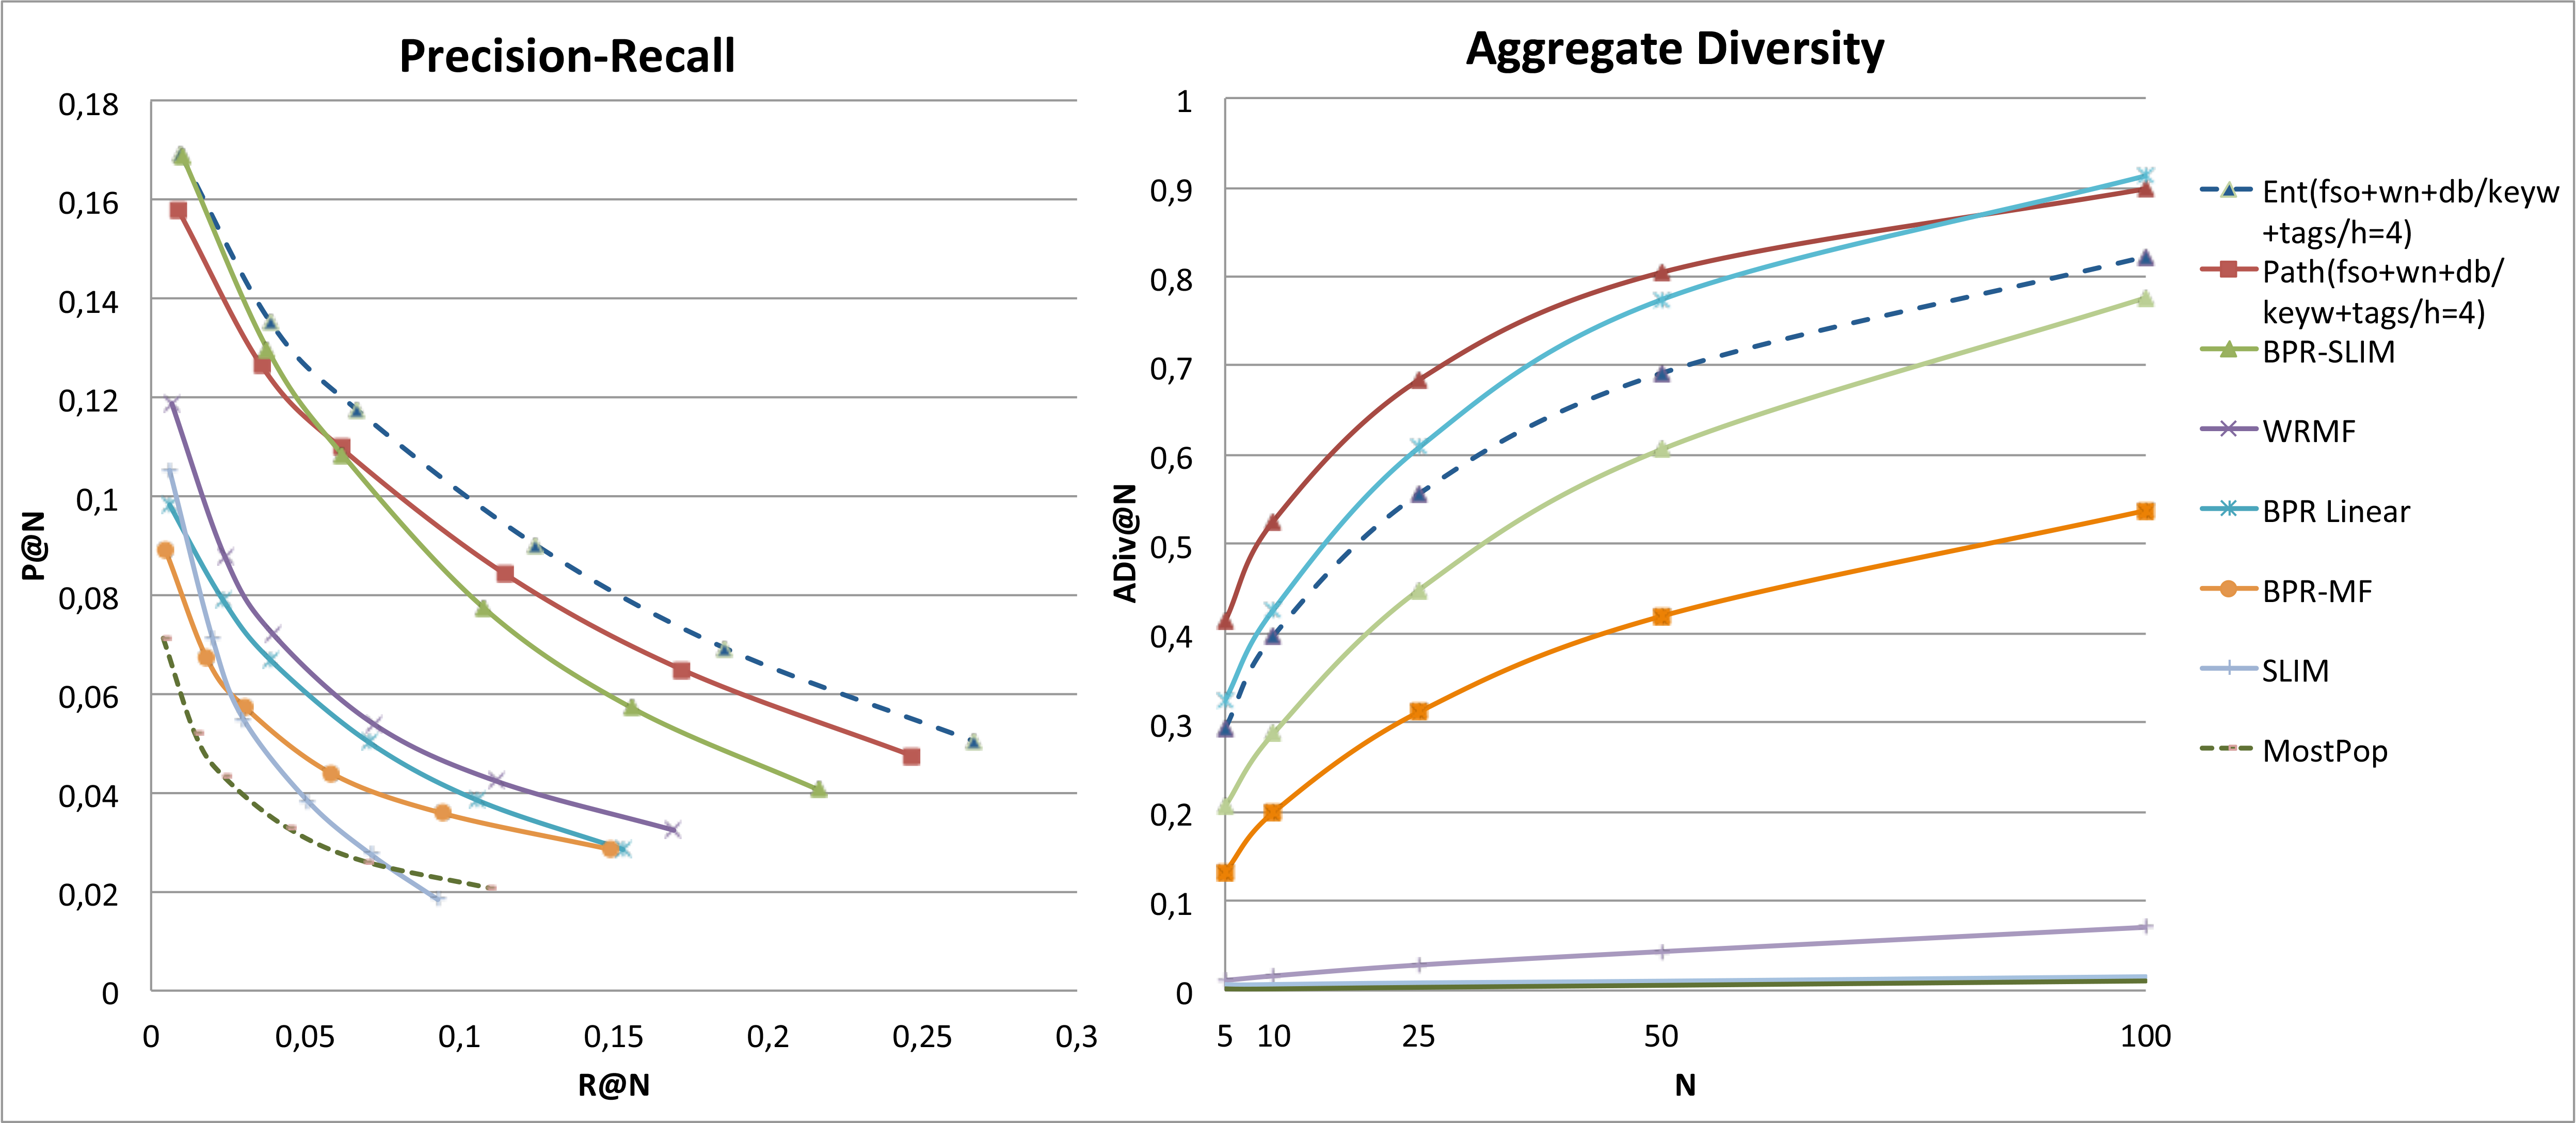
\includegraphics[width=\textwidth]{ch07_graph-rec_pics/pr_adiv_fr.png}
	\end{subfigure}
	\begin{subfigure}[b]{\textwidth}
		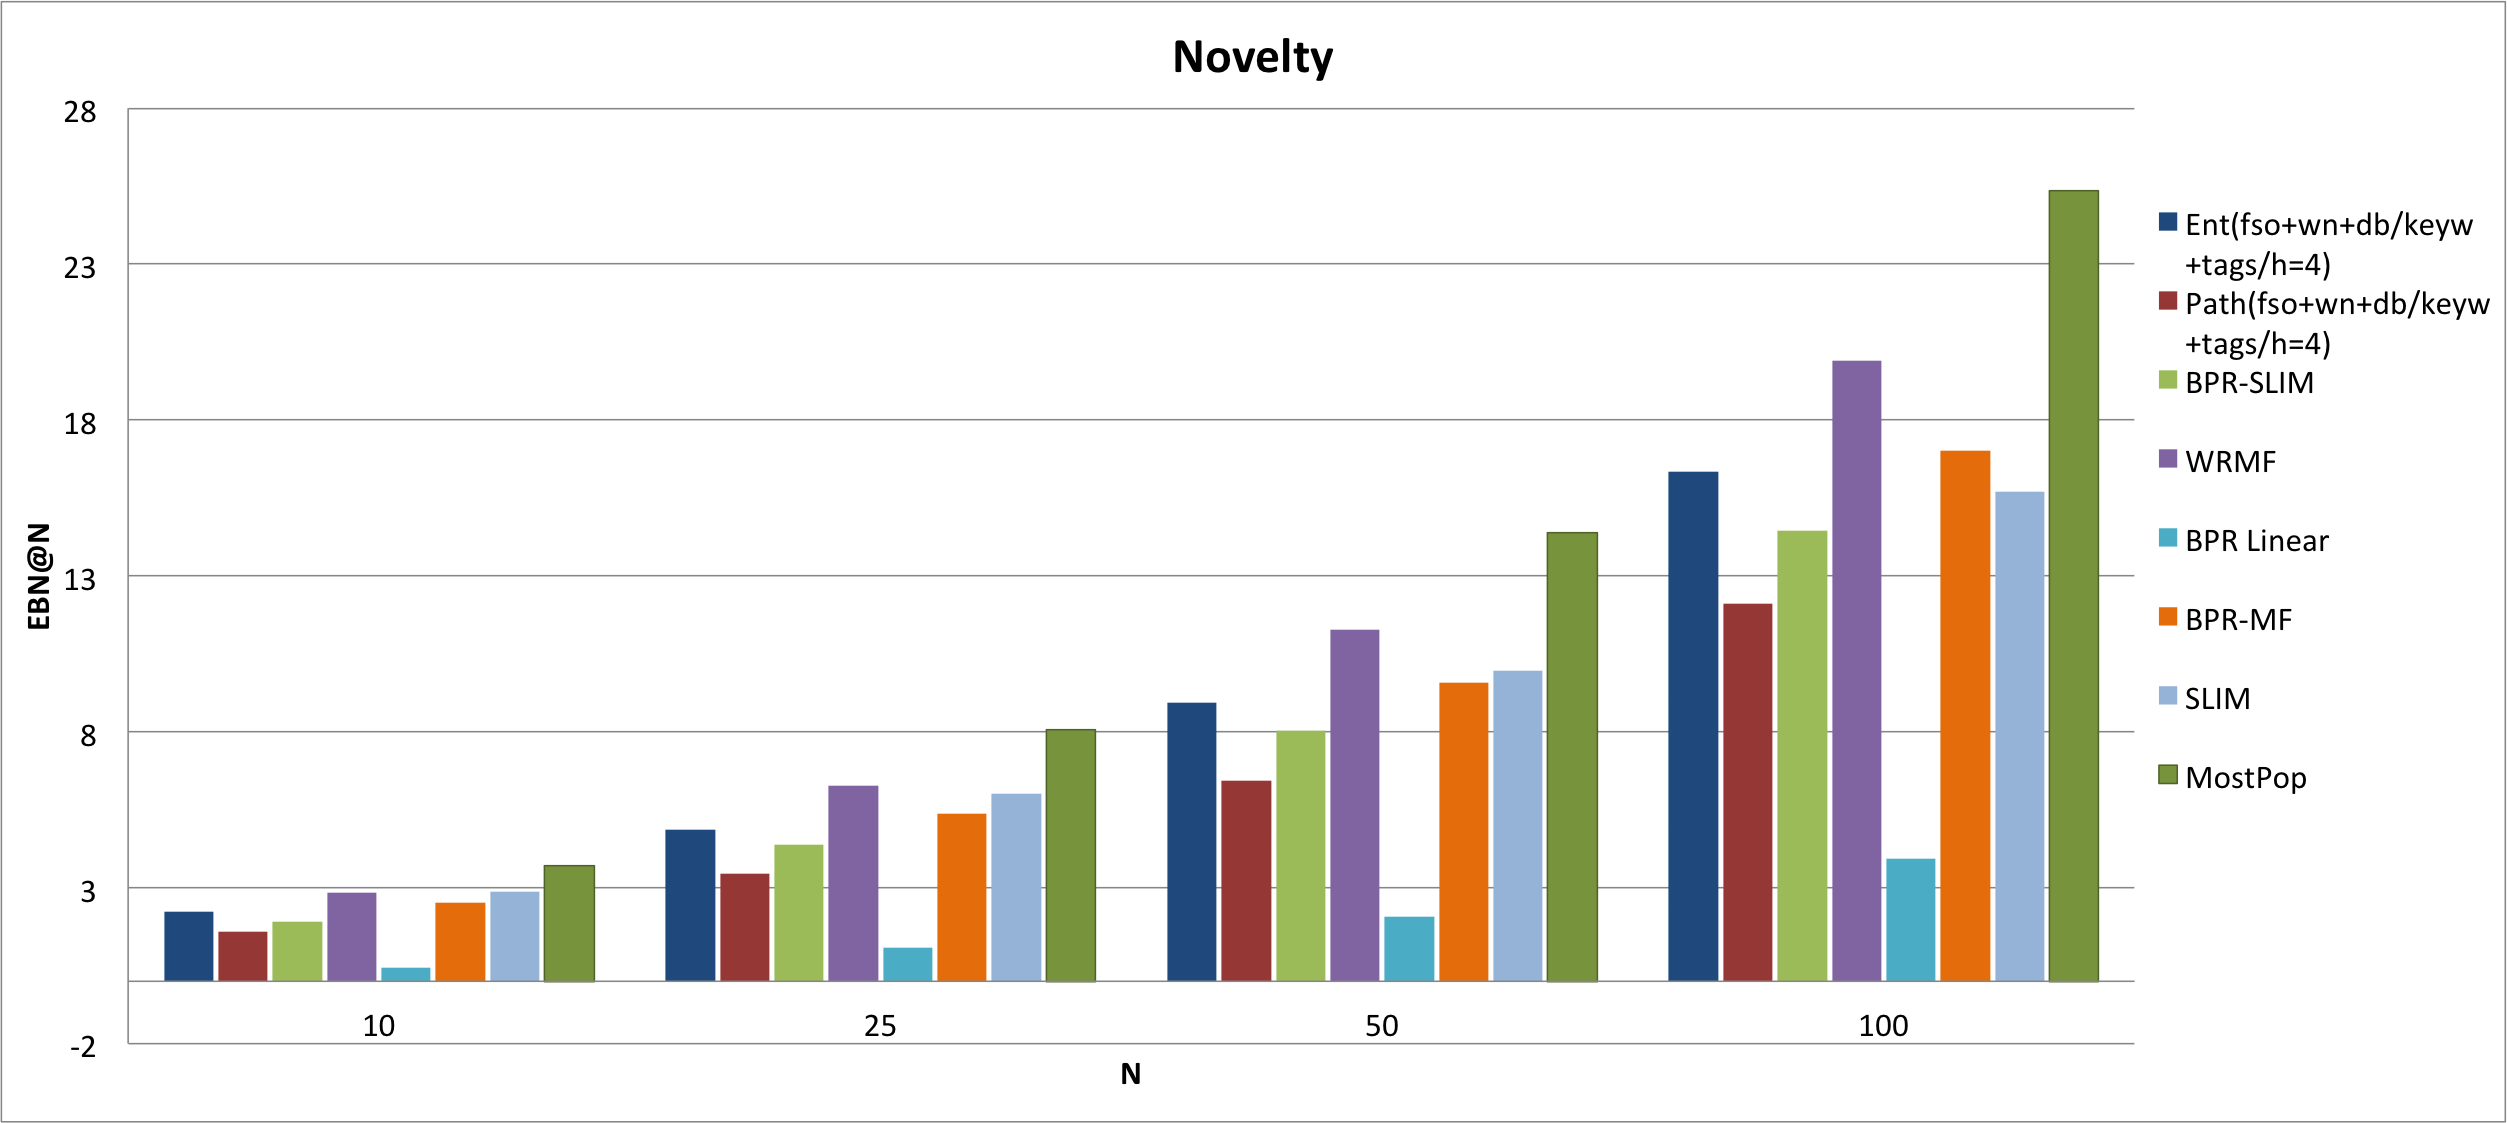
\includegraphics[width=\textwidth]{ch07_graph-rec_pics/nov_fr.png}
	\end{subfigure}
	\caption{Precision-Recall, Novelty and Aggregate Diversity plots in Freesound dataset\label{fig:graph-rec:accur}}
\end{figure*}
%%%%%%%%%%%%%%%%%%%%%%%%%%%%%%%%%%%%%%%%%%%%%%%%%%%%%%%%%%%%%%%%%%%%%%%%%%%%%%%%%%%%%
%%%%%%%%%%%%%%%%%%%%%%%%%%%%%%%%%%%%%%%%%%%%%%%%%%%%%%%%%%%%%%%%%%%%%%%%%%%%%%%%%%%%%
%\begin{figure*}
%	\centering
%	\subfigure{\includegraphics[width=1\textwidth]{ch07_graph-rec_pics/prec_rec.png}}
%	\subfigure{\includegraphics[width=1\textwidth]{ch07_graph-rec_pics/nov.png}}
%	\subfigure{\includegraphics[width=1\textwidth]{ch07_graph-rec_pics/adiv.png}}
%	\caption{Precision-Recall, Novelty and Aggregate Diversity plots\label{fig:graph-rec:accur}}
%\end{figure*}
%%%%%%%%%%%%%%%%%%%%%%%%%%%%%%%%%%%%%%%%%%%%%%%%%%%%%%%%%%%%%%%%%%%%%%%%%%%%%%%%%%%%%%
%In order to evaluate the effectiveness in terms of ranking accuracy of \framechapter we compared it with several state of the art recommendation algorithms:
%\vcoinline{cf focus too much on popular items, instead our approach is able to explore long tail items.}
We compared our approach with several state of the art recommendation algorithms. 
%\begin{scriptsize}
%\begin{itemize}
\texttt{MostPop} is a popularity-based baseline which provides the same recommendation to all users based on the global popularity of items. 
\texttt{BPR-MF} \citep{RendleFGS09} is a matrix factorization-based method optimized with Bayesian Personalized Ranking optimization criterion.
\texttt{WRMF} is a weighted matrix factorization method \citep{Hu2008}.
\texttt{SLIM} \citep{Ning2012} uses a Sparse Linear method for learning a sparse aggregation coefficient matrix.
\texttt{BPR-SLIM} is similar to \texttt{SLIM} but it uses the BPR optimization criterion.
\texttt{BPR Linear} is a hybrid matrix factorization method able to chapter with sparse datasets \citep{GantnerDFRS10}. We used keywords and tags as item attribute data. 
The computation of the recommendations for all these comparative algorithms has been done with the publicly available software library \textit{MyMediaLite}\footnote{\url{http://www.mymedialite.net/}.}.
%\citep{Gantner2011MyMediaLite}

Figure \ref{fig:graph-rec:accur} shows precision-recall, novelty and aggregated diversity plots. In those plots we report the competitive algorithms used for comparison and the \texttt{Ent(fso+KB/kw+tag/h=4)} and \texttt{Path(fso+KB+kw+tag/h=4)} configurations which we chose as representative for our approach due to its performances in terms of novelty and aggregate diversity. 
\\With reference to the accuracy results we notice that our two approaches largely outperforms the others. The only method which is close to the approaches we propose is \texttt{BPR-SLIM} which slightly outperforms \texttt{Path(fso+KB+kw+tag/h=4)} for low values of recommendation list length ($N=5,10$). %All differences between our approach and the other methods are statistically significant ($p<0.01$) according to the paired t-test.
%Regarding our approach, the Entity-based mapping slightly outperfoms the Path-based mapping as already discussed in Section \ref{sem_eval}. 
With respect to the Novelty plot, our approach has much better novelty than all the other collaborative filtering algorithms but \texttt{BPR Linear} which however have much lower accuracy. 
Our approach outperforms most of the collaborative filtering algorithms in terms of aggregated diversity. It is able to achieve a coverage of almost 80\% and 90\% for $N=50$ and $N=100$, respectively. The approach closer to ours is \texttt{BPR Linear} that for $N=100 $ reaches same performances. Also, \texttt{BPR-SLIM} and \texttt{BPR-MF} have acceptable diversity results. Instead, all the others have very low diversity results meaning that they focus mostly on a few specific items and recommend them to all users indiscriminately. 
\\Summing up, the experimental results show that our approach is able to give more accurate and at the same time less popular recommendations, than collaborative filtering methods. It is able to better find good recommendations in the long tail. 
Effective recommendation systems should promote novel and relevant items taken primarily from the tail of the distribution. 
In addition, our approach shows much higher aggregated diversity which can be seen as a higher personalization of the system. 

\subsection{Music recommendation experiment}
The recommendation algorithms we propose have been further validated on the Last.fm dataset. We performed the same experiments on this dataset to assess the applicability of the approach to other musical contexts.
%To confirm the obtained results and its applicability to other musical contexts, we performed a second experiment on the Last.fm dataset using the same set of feature vector variants and competitor approaches. %Results on the evaluation of the semantic item description enhancement are shown in Table~\ref{tbl:graph-rec:Res_sf}.
%, whilst the comparison with other methods is shown in Figure~\ref{fig:graph-rec:accur_sf}. 
%%%%%%%%%%%%%%%%%%%%%%%%%%%%%%%%%%%%%%%%%%%%%%%%%%%%%%%%%%%%%%%%%%%%%%%%%%%%%%%%%%%%
\begin{table}
\scriptsize
	%[!htb]
	%\tbl{Last.fm Results}{%
%	\scriptsize
	\label{tbl:graph-rec:Res_sf}
	\begin{tabular}{l l c c c c c c }
		\toprule
		\textbf{Approach} & \textbf{Enrichment} & \textbf{h-hops} &  \textbf{MRR} &  \textbf{P@10} & \textbf{R@10} & \textbf{EBN@10}  & \textbf{ADiv@10}\\
		\midrule
		Ent & KB/tag & h=2 & \textbf{0.612} & 0.321 & \textbf{0.122} & 2.414 & 0.357 \\
%		Ent(KB/tag/h=2) & \textbf{0.612} & 0.321 & \textbf{0.122} & 2.465 & 0.342 \\
		Ent & KB/tag & h=3 & \textbf{0.612} & 0.319 & 0.121 & 2.383 & 0.374 \\
		Ent & KB/tag & h=4 & 0.599 & 0.314 & 0.119 & 2.356 & 0.389 \\
		Ent & KB/kw+tag & h=3 & 0.604 & 0.315 & 0.114 & 2.448 & 0.316 \\
		Ent & KB/kw+tag & h=4 & 0.601 & 0.312 & 0.113 & 2.424 & 0.331 \\
		Path & KB/tag & h=3 & 0.570 & 0.287 & 0.108 & 2.112 & 0.479 \\
		Path & KB/tag & h=4 & 0.537 & 0.260 & 0.097 & \textbf{1.911*} & \textbf{0.544*} \\
		Path & KB/kw+tag & h=3 & 0.570 & 0.289 & 0.104 & 2.173 & 0.411 \\
		Path & KB/kw+tag & h=4 & 0.537 & 0.259 & 0.093 & 1.942 & 0.484 \\
		\midrule
		Collab & & & 0.597 & 0.313 & 0.113 & 2.664 & 0.240 \\	
		Ent-noCol & KB/tag & h=3 & 0.292 & 0.114 & 0.043 & 0.983 & 0.703 \\
		Path-noCol & KB/tag & h=3 &0.285  & 0.113 & 0.043 & \textbf{0.981} & \textbf{0.736} \\
		VSM & tags & h=1 & 0.610 & \textbf{0.322} & \textbf{0.122} & 2.454 & 0.346 \\
		VSM & keyw & h=1 & 0.599 & 0.309 & 0.112 & 2.642 & 0.249 \\
%		VSM tags - noCol & 0.127 & 0.048 & 1.050 & \textbf{0.757} \\	
		\bottomrule		
	\end{tabular}
	\caption[Accuracy, Novelty and Aggregate Diversity results for different versions of the Last.fm dataset.]{Accuracy, Novelty and Aggregate Diversity results for different versions of the Last.fm dataset. Best values in each column are in bold. The * symbol indicates best values for hybrid and collaborative configurations. 
	}
\end{table}
%%%%%%%%%%%%%%%%%%%%%%%%%%%%%%%%%%%%%%%%%%%%%%%%%%%%%%%%%%%%%%%%%%%%%%%%%%%%%%%%%%%%

\subsubsection{Evaluation of the semantic item description enhancement}\label{sem_eval}
As we may notice from the results shown in Table~\ref{tbl:graph-rec:Res_sf}, Entity-based embedding, \texttt{Collab}, and \texttt{VSM tags} approaches have very similar performance in terms of precision and recall. The first two Entity-based embedding variants have slightly higher MRR than \texttt{VSM tags}, meaning that they better locate relevant items in the top positions. Analogously to the previous sounds recommendation task, the approaches exploiting semantic expansion outperform the others in terms of novelty and aggregated diversity. The same tendency of the previous experiment is observed with the Entity-based and Path-based item neighborhood mappings. The Path-based approaches have lower precision, but much better novelty and aggregated diversity. Moreover, it is very interesting to observe that for both embedding options if we expand the graph by means of farther entities (h=4) precision decreases whilst novelty and diversity improve. It is noteworthy that differently from the results of the Freesound experiment, here we obtain higher accuracy with the approach that uses only tags and not keywords. Our interpretation of this trend is that, as shown in Table~\ref{tbl:graph-rec:datasets}, the number of tags in the Freesound dataset is somehow scarce, and the addition of keywords taken from the textual descriptions improves the annotation of the items. On the other side, in the Last.fm dataset, the set of tags is already very rich, then the addition of keywords introduces noise within the items description thus deteriorating the accuracy of recommendations. 
Also in this experiment we can observe that when no collaborative features are used, accuracy is significantly worse even if novelty and diversity seem to be better. 
We may confirm from results in both experiments that collaborative features are a very strong signal for the accuracy of the recommendations. Nonetheless, the inclusion of semantic features allows the system to further improve accuracy and provide novel and diverse recommendations, thus better leveraging the long tail. %All the differences between the hybrid graph embeddings and the other baselines are statistically significant ($p<0.01$) according to the paired t-test.
%%%%%%%%%%%%%%%%%%%%%%%%%%%%%%%%%%%%%%%%%%%%%%%%%%%%%%%%%%%%%%%%%%%%%%%%%%%%%%%%%%%%%
\begin{figure*}
	\centering
	\begin{subfigure}[b]{1\textwidth}
		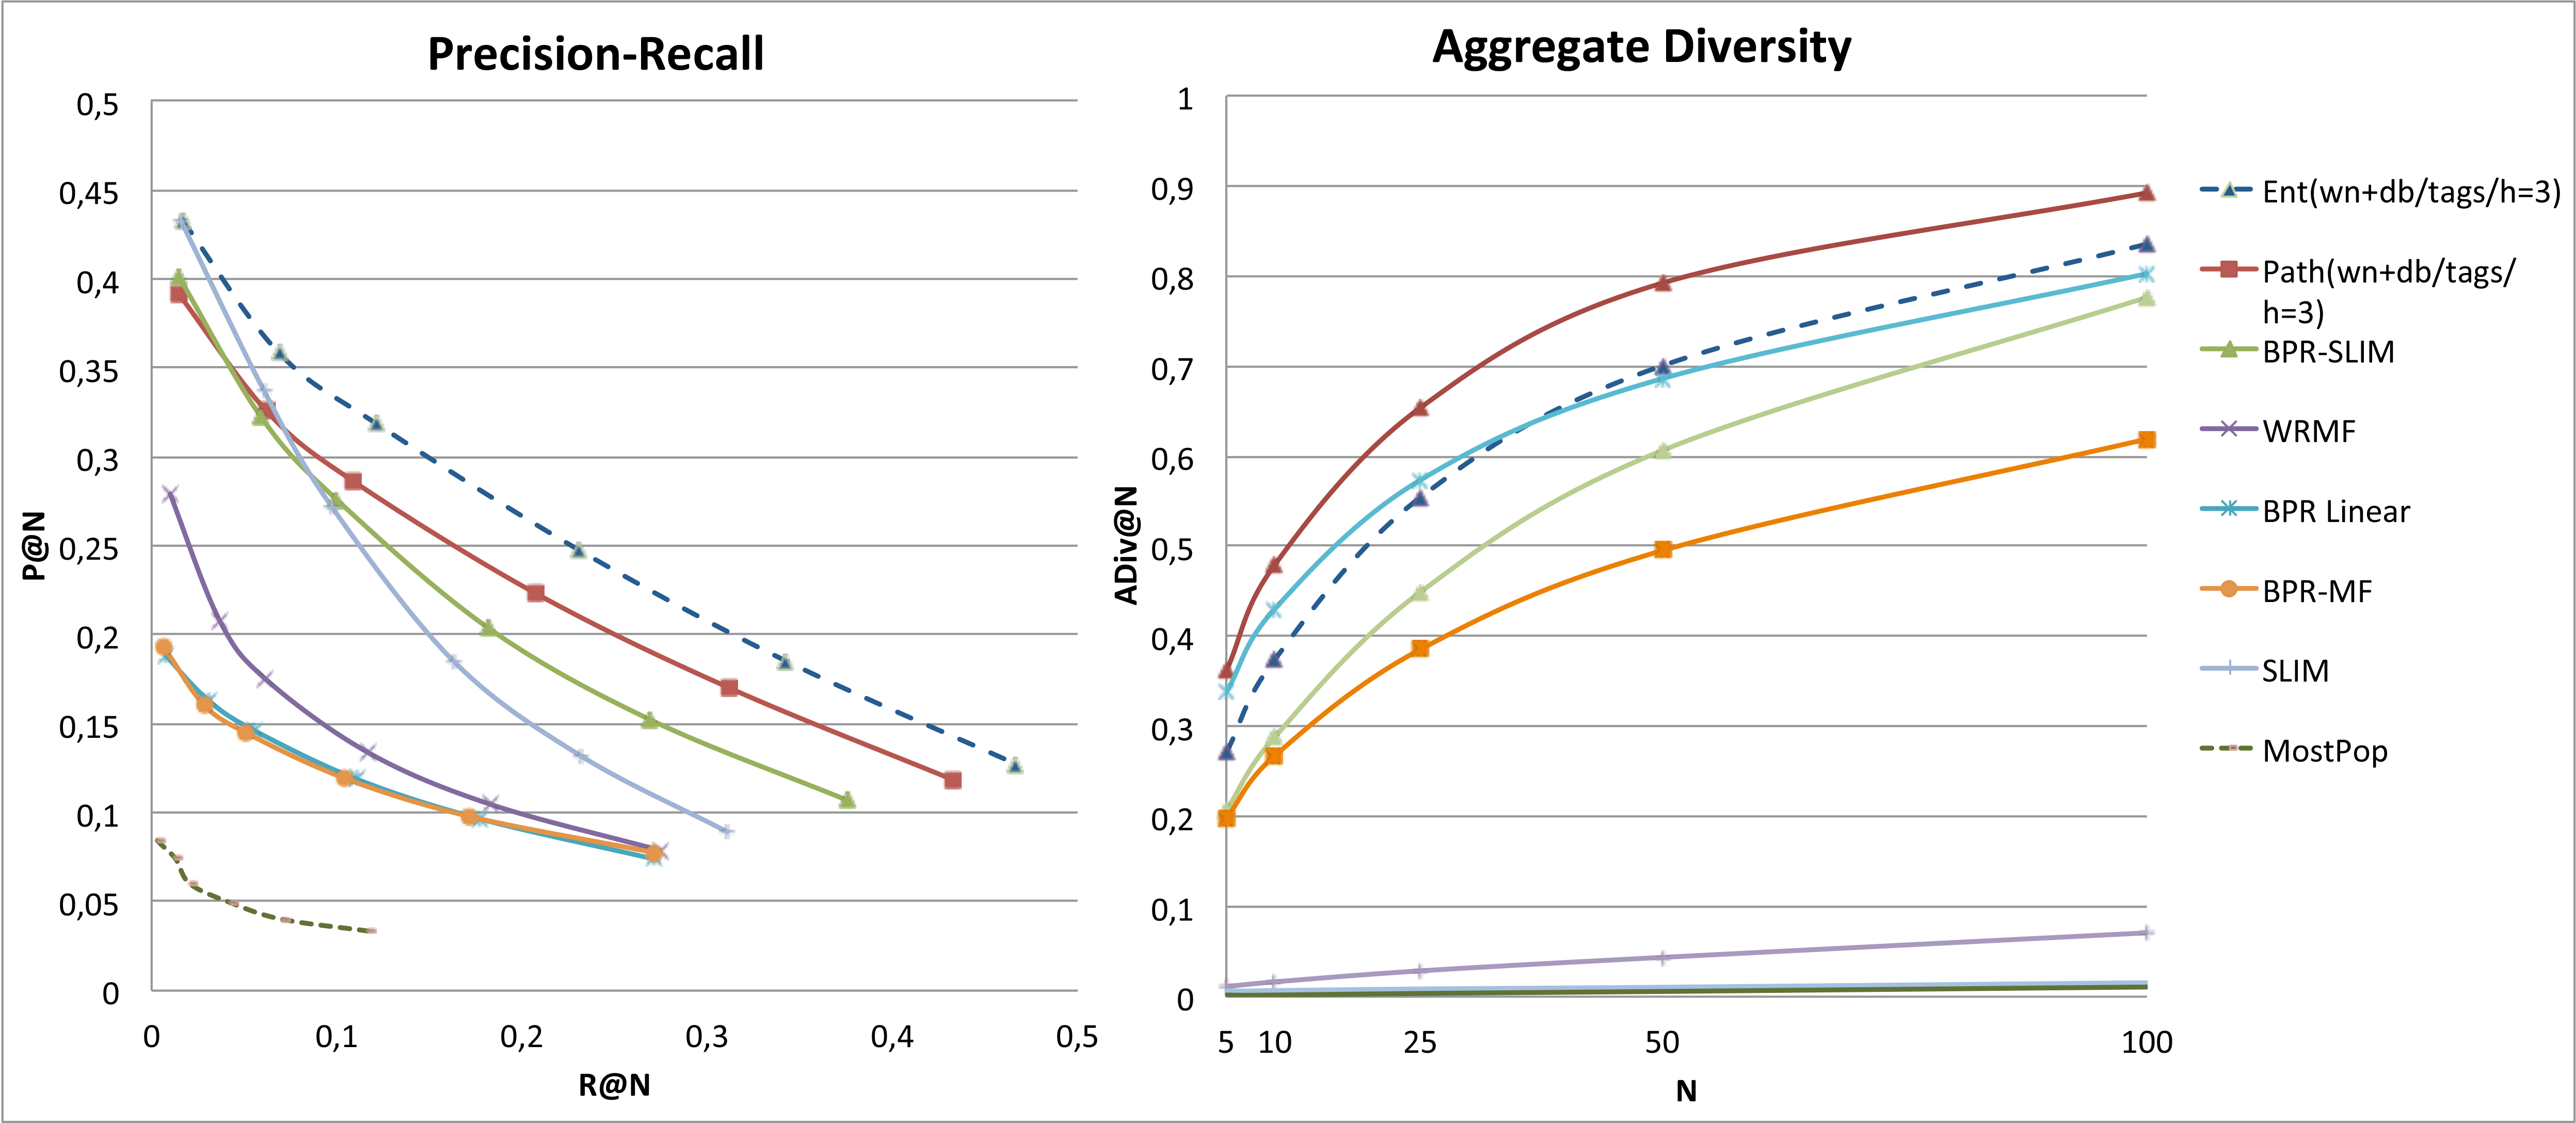
\includegraphics[width=\textwidth]{ch07_graph-rec_pics/pr_adiv_lf.png}
	\end{subfigure}
	\begin{subfigure}[b]{1\textwidth}
		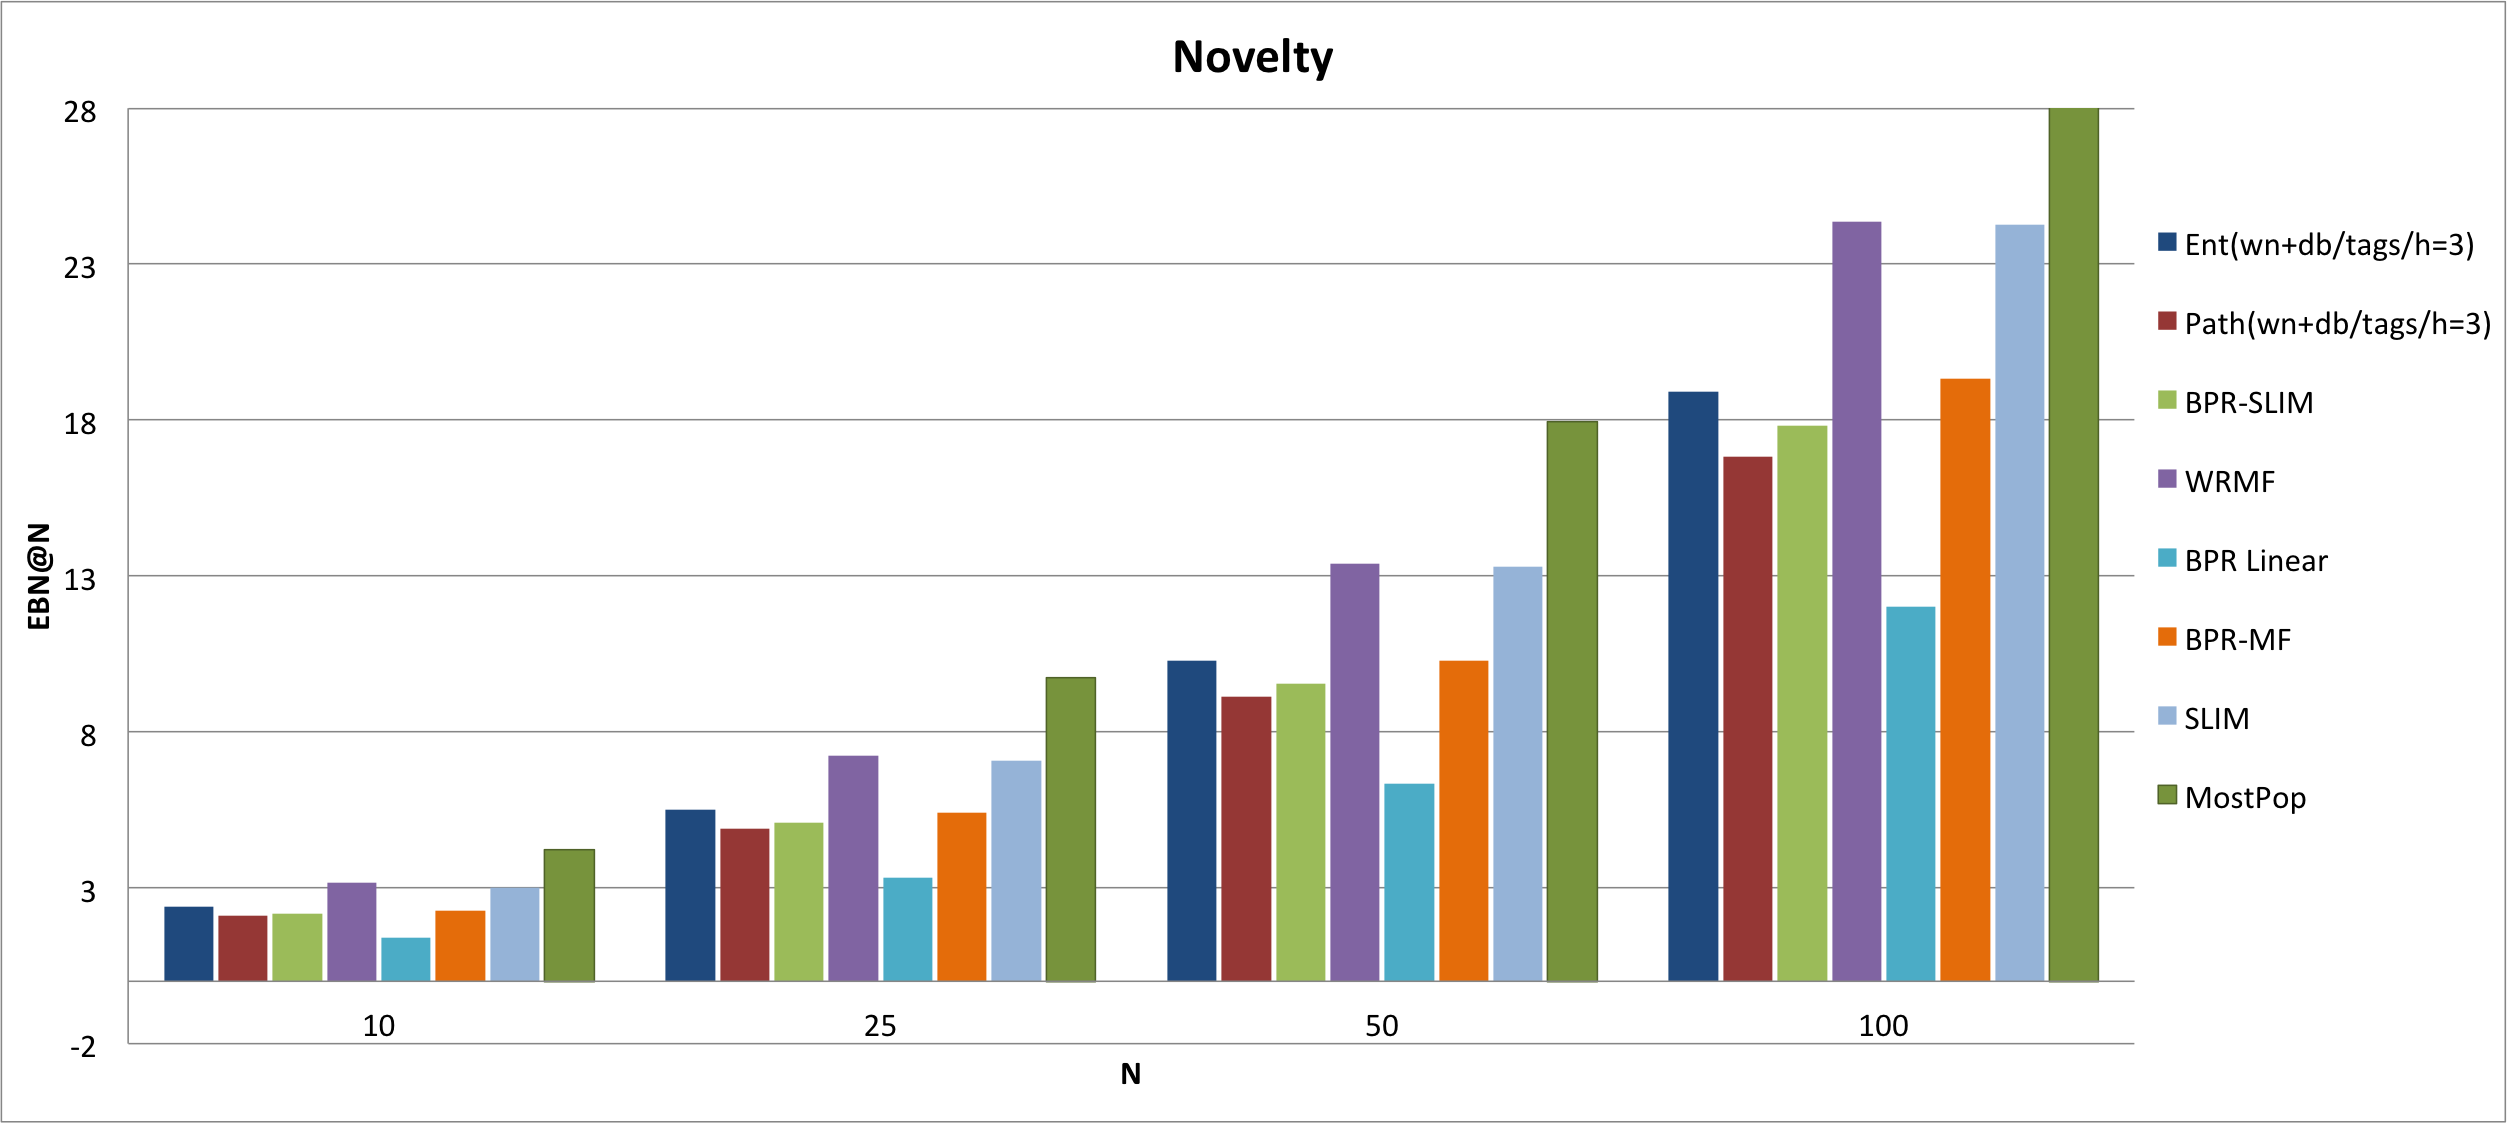
\includegraphics[width=\textwidth]{ch07_graph-rec_pics/nov_lf.png}
	\end{subfigure}
	\caption{Precision-Recall, Novelty and Aggregate Diversity plots in Last.fm dataset\label{fig:graph-rec:accur_sf}}
\end{figure*}
%%%%%%%%%%%%%%%%%%%%%%%%%%%%%%%%%%%%%%%%%%%%%%%%%%%%%%%%%%%%%%%%%%%%%%%%%%%%%%%%%%%%%

\subsubsection{Comparison with other methods}\label{comp}
We compared our approach with the same set of state of the art algorithms presented in the sound recommendation experiment. Based on the observations made in the previous paragraph, we used for this experiment only tags as item attribute data for \texttt{BPR Linear}.
Figure \ref{fig:graph-rec:accur_sf} shows precision-recall, novelty and aggregated diversity plots of the comparison with the other methods. We compare the competitive algorithms with the \texttt{Ent(KB/tag/h=3)} and \texttt{Path(KB/tag/h=3)} configurations which in this scenario results to be the most representative for our approach. 
Results are pretty similar to the ones observed in the sound recommendation experiment. Our two approaches largely outperforms the others in terms of accuracy. \texttt{BPR-SLIM} and \texttt{SLIM} have performance similar to our Entity-based mapping approach for low values of recommendation list length (N = 5, 10), and slightly higher that the Path-based one. %All differences between our approaches and the other methods are statistically significant ($p<0.01$) according to the paired t-test. 
Our approaches have much better novelty results than all other collaborative filtering algorithms but \texttt{BPR Linear}, which again has much lower accuracy. In terms of aggregated diversity, our approach outperforms most of the collaborative filtering algorithms. \texttt{BPR Linear} achieves similar diversity, but much lower accuracy.
Summing up, our approach is able to recommend less popular items with higher accuracy than other collaborative filtering algorithms also in this recommendation scenario. Therefore, our approach is able to improve the level of personalization of the recommended items, and  better explore the long tail also for songs recommendation.



\section{Conclusion}
\label{sec:graph-rec:conclusion}
We have presented a hybrid approach to recommend musical items, i.e. sounds and songs, by exploiting the information encoded within a knowledge graph. We conducted various experiments on two different datasets, the one of sounds coming from Freesound.org, the other one of songs gathered from Last.fm and Songfacts.com. They may be considered as representative of the two classes of users we find in the music domain: producers looking for sounds to create new music and consumers looking for new songs to listen to.

Information coming from item descriptions and tags have been %structured by means of an ontology and then further 
enriched with data coming from two external knowledge repositories: DBpedia and WordNet. Entity Linking tools have been adopted to extract relevant entities from textual sources associated to musical items, namely tags and text descriptions, thus creating a new graph encoding the knowledge associated to users, items and their mutual interactions. We then developed a recommendation engine that combines different features, that is semantic content-based ones extracted from the resulting knowledge graph and collaborative information from implicit user feedback. An evaluation with two explicit feature mappings, \textit{entity-based item neighborhood} and \textit{path-based item neighborhood}, has been conducted on both datasets in order to asses the performance of the system in terms of accuracy, diversity and novelty. 

Experimental results in sounds and songs recommendation show that the proposed approach is able to improve the quality of the recommended list with respect to state of the art collaborative filtering algorithms and with respect to other content-based baselines. Our results also show that the data related to the music knowledge domain encoded in freely available datasets such as DBpedia or WordNet have reached a quality level that makes possible its usage in the creation of recommendation engines whose target are either music producers or music consumers. The semantic enrichment of the initial knowledge graph performed by means of entity linking techniques is a good choice to boost the performances of the system in terms of novelty and aggregate diversity. A knowledge-based approach can improve the degree of personalization in the recommendations of musical items from various points of view such as prediction accuracy, catalog coverage and promote long tail recommendations. We have presented a methodology that achieves these objectives by combining semantic knowledge with collaborative information. 

Summing up, knowledge graphs can be a useful tool when properly leveraged within recommender systems for musical items. Indeed, the graph-based nature of the information they contain, on the one hand, makes possible a linkage to other graphs thus resulting in an easy plugging of new content-based data. On the other hand, by exploring the graph new connections and commonalities between items and users can be discovered and exploited while computing the recommendation list.


%\\As future chapter we are currently planning to integrate the proposed algorithm into Freesound for computing sound recommendation and perform an experimental evaluation with real users. In addition, we want to evaluate the proposed approach on different domains to generalize the results about the usage of the semantic feature expansion to improve aggregate diversity and novelty. 
\cleartorecto%!TEX root = ../thesis_a4.tex

\part{Representation Learning}
\label{part:multimodal-deep}

\chapter{Cold-start Music Recommendation}
\label{sec:cold-rec}

\section{Introduction}\label{sec:cold-rec:intro}
\label{sec:cold-rec:intro}

%It is common for online music streaming services nowadays to offer ever-growing catalogs with dozens of millions of music tracks.
%Since manually managing these large libraries is not feasible due to size constraints, automatic exploration and exploitation of large-scale music collections has been an active area of research in recent years \cite{schedl2014music}.
%While several existing algorithmic techniques are able to produce successful recommendations for popular content \cite{Koren2009}, the exploration of new or \emph{undiscovered} artists (i.e., the long tail \cite{Celma2010}) remains a major challenge that we aim to address.

%Recommender systems can be broadly classified into collaborative filtering (CF), content-based, and hybrid methods. CF methods \cite{Koren2009} use the item-user feedback matrix and predictions are based on the similarity of user or item profiles. Matrix factorization techniques are currently CF state-of-the-art \cite{Koren2009}. 

An increasing amount of digital music is being published daily. Music streaming services often ingest all available music, but this poses a challenge: how to recommend new artists for which prior knowledge is scarce? In this chapter we aim to address this so-called cold-start problem by combining text and audio information with user feedback data using deep learning architectures. 

%Our method is divided into three steps. First, artist embeddings are learned from biographies by combining semantics, text features, and aggregated usage data. Second, track embeddings are learned from the audio signal and available feedback data. Finally, artist and track embeddings are combined in a multimodal network. Results suggest that both splitting the recommendation problem between feature levels (i.e., artist metadata and audio track), and merging feature embeddings in a multimodal approach improve the accuracy of the recommendations.

Social tags have been extensively used as a source of artist content features to recommend music \citep{Knees2013}. However, these tags are usually collectively annotated, which often introduce an artist popularity bias \citep{Turnbull2008}.
Artist biographies and press releases, on the other hand, do not necessarily require a collaborative effort, as they may be produced by artists themselves. 
However, they have seldom been exploited for Music Recommendation.
Part of this chapter focuses on learning artist features from these biographies.
Furthermore, we also make use of audio signals, since these are generally always available and have shown to be helpful when recommending music in the long tail \citep{Oord2013}.

According to \cite{gulccehre2016knowledge}, composing simpler tasks is more likely to yield effective local minima for neural networks. In addition, as stated in \cite{larochelle2009exploring}, directly training all the layers of a deep network together make it difficult to exploit all the extra modeling power of a deeper architecture. 
Therefore, we decided to separate the problem of Music Recommendation into artist and song levels.
Artist feature embeddings are learned from artist metadata in an artist recommendation scenario.
Track feature embeddings are learned from audio signals in a song recommendation scenario.
In both cases, a hybrid recommendation approach is used based on learning attribute-to-feature mappings \citep{GantnerDFRS10}.
This method addresses the lack of feedback for uncommon items in two steps: (1) factorizing the collaborative matrix, and (2) learning a mapping between item content features and item latent factors \citep{Oord2013,Bansal2016}.
Lastly, both feature embeddings are combined in a multimodal network to predict song recommendations of cold-start artists.
We show how dividing the problem into artists and songs, and combining text and audio in a multimodal approach yields improved recommendations.

The rest of the chapter is organized as follows. First, we describe in detail the recommendation approach (Section~\ref{sec:cold-rec:approach}). Then, we describe the architectures used to obtain artist text embeddings (Section~\ref{sec:cold-rec:text}), track audio embeddings (Section~\ref{sec:cold-rec:audio}), and their combination (Section~\ref{sec:cold-rec:multimodal}). Experiments and evaluation results are reported in Section~\ref{sec:cold-rec:experiments}, and the chapter ends with a discussion about our findings (Section~\ref{sec:cold-rec:conclusions}).


%For the sake of reproducibility, source code and data splits used in the experiments have been released\footnote{https://github.com/sergiooramas/tartarus}.
%Our main contributions in this work are summarized as follows:
%\begin{itemize}
%\item{Method to enrich artist biographies with semantic information leveraging an external Knowledge Base.}
%\item{Dividing the problem of Music Recommendation into artist and song levels to obtain better performance.}
%\item{A multimodal deep learning pipeline for Music Recommendation that combines audio with text and yields improved results.}
%\item{The release of an extended version of the Million Song Dataset with artist biographies and tags.}
%\end{itemize}


%Almost every artist has a biography or a press release, either self-written or written by others, and they are typically available on the web. For these reasons we focus our study in the learning of artist features from artist biographies.

% Content-based Music Recommendation, where relevant information is extracted directly from the audio signal, 


% Music information of popular music can be structured in three different levels: artist, album and song. 
% Accordingly, the Music Recommendation problem can be divided into different phases, based on the available information in every level.
% In this work, we first separate the problem of song recommendation in two phases, related to the artist and song levels.
% Artist feature vectors are learned from artist metadata in an artist recommendation scenario.
% Song feature vectors are learned from audio signals in a song recommendation scenario.
% Lastly, both feature vectors are combined in a multimodal deep network to predict song recommendations. 

% To obtain artist and song feature vectors and compute the recommendations, we follow a hybrid recommendation approach based on learning attribute-to-feature mappings \citep{ Learning attribute-to-feature mappings for cold-start recommendations}. 
% This method addresses the cold-start problem in two steps: (1) factorizing the collaborative matrix, and (2) learning a mapping between item content features and item latent factors. 
% Similar approaches have been proposed for recommender systems, using deep networks in the learning process. For instance, in \cite{dielemann}, the audio signal is used to learn song latent factors, whereas in \cite{recsys2015} latent factors are learned from text for scientific paper recommendation. 
% In this work, we learn song and artist feature vectors separately using deep architectures, and further combine them in a multimodal deep network. 
% We show how dividing the problem into music levels, and combining audio and text in a multimodal approach yields better recommendations. % no se yo si high quality results

%We first extract semantic information from several artist biographies, and use these data to learn a latent representation of each artist of the Million Song Dataset (TODO: cite MSD)(TODO: Is it really each MSD artist?).
%Secondly, we train another model using audio signals as input to predict the factorized space of each of the tracks in the set.
%Finally, we combine the output of the two previously trained models into a third network, resulting in a significant increase in performance when compared to audio- or text-only models.

%In this work we show how the combination of audio and text in a multimodal approach using deep architectures yields higher quality results.
%We first extract semantic information from several artist biographies, and use these data to learn a latent representation of each artist of the Million Song Dataset (TODO: cite MSD)(TODO: Is it really each MSD artist?).
%Secondly, we train another model using audio signals as input to predict the factorized space of each of the tracks in the set.
%Finally, we combine the output of the two previously trained models into a third network, resulting in a significant increase in performance when compared to audio- or text-only models.

\section{Recommendation Approach}
\label{sec:cold-rec:approach}

% In this work, a method to recommend items that are new to a recommender system is proposed. 
% More specifically, we aim to address the cold-start problem: where little to none collaborative information is available when producing recommendations.

% This scenario is often referred to as the cold-start problem.
% More specifically, we want to recommend songs whose artist was not previously in the catalog, which means that the system does not have any collaborative information about other songs by the same artist. This problem can be considered as an extreme case of the cold-start scenario.

% To produce Music Recommendations in the long tail, we propose the following framework.
% Given the set of artist features $A_{s}$ of a song $s$ with $A_{s}={a_{1},a_{2},...,a_{n}}$, and the set of track features $T_{s}$ of $s$ with $T_{s}={t_{1},t_{2},...,t_{m}}$, the complete feature set of $s$ is defined as the aggregation of its artist and track features $F_{s} = A_{s} \cup T_{s}$.
To produce cold-start Music Recommendations, we propose the following framework.
Given the set of artist features $A_{s}$ of a song $s$, and the set of track features $T_{s}$ of $s$, the complete feature set of $s$ is defined as the aggregation of its artist and track features $F_{s} = A_{s} \cup T_{s}$.
% This aggregated set of features is typically used as input in content-based and hybrid music recommender systems (TODO: cite).

Given the heterogeneity of these two feature sets (audio and text), a learning process involving them may under-explore one of the modalities, as the stronger modality may dominate quickly. 
To ensure that the variability of the input data is fully represented, we divide the problem into three phases (see Figure~\ref{fig:approach}). First, we aggregate the collaborative information of all songs of the same artist, and learn an artist feature embedding $A'_{s}$ from $A_{s}$ in an artist recommendation scenario. Second, we learn a track feature embedding $T'_{s}$ from $T_{s}$ in a pure audio-based recommendation scenario. Third, we combine both feature embeddings $A'_{s}$ and $T'_{s}$ in a multimodal network and compute song recommendations. 

Since songs from the same artist share the same set $A_{s}$, if different songs from the same artist appear in multiple sets (e.g., train and test), a problem of overfitting may arise \citep{Flexer2007ACL}.
To approach this issue, we use non-overlapping artists across the train, validation, and test sets.

%Since songs from the same artist share the same set $A_{s}$, two problems may arise: (1) the learning process involved with the recommender system might not be properly optimized, and (2) if different songs from the same artist appear in multiple sets (e.g., train and test), a problem of overfitting may arise \citep{Flexer2007ACL}.

%To address (1), we divide the problem into three phases (see Figure~\ref{fig:approach}). First, we aggregate the collaborative information of all songs of the same artist, and learn an artist feature embedding $A'_{s}$ from $A_{s}$ in an artist recommendation scenario. Second, we learn a track feature embedding $T'_{s}$ from $T_{s}$ in a pure audio-based recommendation scenario. Third, we combine both feature embeddings $A'_{s}$ and $T'_{s}$ in a multimodal network and compute song recommendations. To approach (2), we use non-overlapping artists across the train, validation and test sets.

\begin{figure}[!htp]
\centerline{
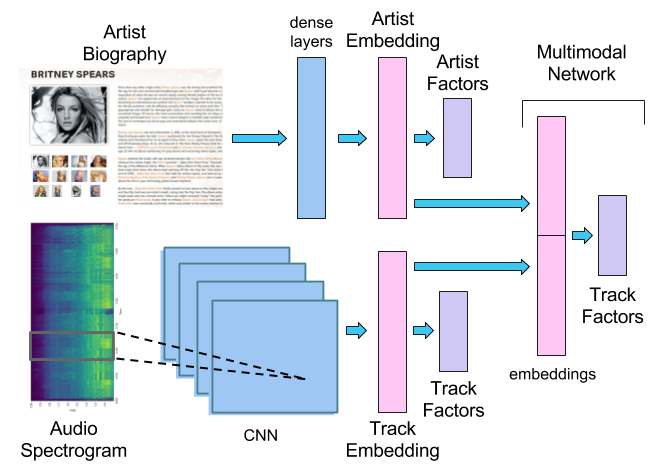
\includegraphics[width=0.75\columnwidth]{ch08_cold-rec_pics/approach.png}}
\caption{Model architecture.}
\label{fig:approach}
\end{figure}

Let $M$ be the matrix of implicit feedback, where $m_{us}$ is the number of play counts for user $u$ on song $s$. 
$M$ is split into $M_{train}$, $M_{val}$ and $M_{test}$, for train, validation and test, respectively, where no artist is shared across sets. 
Factorizing $M_{train}$ using weighted matrix factorization (WMF) \citep{Hu2008} yields $I_{k}$ and $U_{k}$, the $k$ dimensional sets of song and user latent factors, respectively.
We set $k=200$, and apply the alternating least squares (ALS) optimization method.% with the default parameters. 
%, and more explicitly their alternating least squares (ALS) optimization method \cite{}. 


To learn the artist embeddings, we obtain the matrix of artist implicit feedback $R$ from $M$, being $R_{ua} = \sum_{s}m_{us}$ for all songs $s$ from the same artist $a$. This matrix is split into train, validation, and test sets following the same partition of artists made for $M$, and thus keeping the mutual exclusion restriction. 
Latent factors of artists and users are later obtained via WMF. 
Lastly, a deep neural network is trained on the prediction of artist latent factors from artist content features $A$.
On the other hand, the song latent factors are predicted with a deep convolutional network, using $I_{k}$ as training data and the track features $T$ as input (similar to \cite{Oord2013}).
% Given $I_{k}$, a deep neural network is trained on the prediction of song latent factors $I_{k}$ from audio track features $T$.

Once the artist and track models are trained and optimized, we gather the activations from the penultimate layer of each network for all the sets. These activations constitute what we call the artist and track feature embeddings $A'_{s}$ and $T'_{s}$, which are in turn used as input to a third network. 
This final multimodal network is trained on the prediction of song latent factors $I_{k}$ from $S'_{s} = A'_{s} \cup T'_{s}$.
Finally, the list of item recommendations for user $u$ is obtained by ranking the results of computing the dot product between the user latent factor $f_{u} \in U_{k}$ and the set of item factors. %the set of predicted item latent factors in the test set. %This ranking is evaluated in comparison with the ranked list of items for user $u$ present in the test matrix $M_{test}$.


The different architectures used in each one of the three neural networks involved in the approach are described in Sections \ref{sec:cold-rec:text} ,\ref{sec:cold-rec:audio}, and \ref{sec:cold-rec:multimodal}, respectively.
Nevertheless, all networks have a final fully connected layer of 200 units\footnote{to match the dimensions of the factors to be predicted.} with linear activation and l2-normalization. 
In addition, mini batches of 32 items are randomly sampled from the training data to compute the gradient in all networks, and Adam \citep{KingmaB14} is the optimizer used to train the models, with the default suggested learning parameters. 
Given that the output of the architectures are l2-normalized, we use cosine proximity as the loss function, as in \cite{Chollet2016}.

\section{Artist Text Embeddings}\label{sec:cold-rec:text}

% Following the approach defined in Section \ref{}, a matrix of artist and songs is obtained by aggregating the play counts of songs of the same artist present in the MSD. Then, a deep network is trained to learn the artist latent factors from the biography texts. 
In this section we describe two different, competing approaches to exploit artist texts in a deep learning process. %Then, these two approaches are evaluated in an artist recommendation scenario. Finally, artist embeddings are obtained.

\subsection{Semantic enrichment}\label{sec:cold-rec:sem}

We propose a method for enriching artist biographies by associating text fragments with relevant entities defined in online knowledge repositories, and then gathering relevant semantic information about them. For this purpose, we adopted Babelfy \citep{Moroetal2014} and ELVIS (see Section~\ref{sec:linking:elvis}). We use semantic information about the identified entities coming from DBpedia to enrich the biographies. 

As shown in Chapter~\ref{sec:graph-rec}, Entity Linking systems may be useful for Music Recommendation. However, as illustrated in Chapters~\ref{sec:linking} and \ref{sec:kb}, they are not optimized for the music domain, and are prone to errors. The application of a filtering process over the set of identified entities based on their classification within the DBpedia Ontology, has demonstrated its utility to improve music retrieval tasks, such as artist similarity (cf. Section~\ref{sec:similarity:similarity}). Therefore, we only keep entities of classes related to the music domain such as \textit{MusicalArtist}, \textit{Band}, \textit{MusicGenre}, \textit{MusicalWork}, \textit{RecordLabel}, \textit{Instrument}, \textit{Engineer}, and \textit{Place}. Then, we query DBpedia to get all the available information about the filtered entities. From the information gathered, we keep some specific properties for every kind of entity, such as homeTown, instrument, genre or associatedBand for MusicalArtists, writer, producer or recordedIn for MusicalWorks, stylisticOrigin or instrument for MusicGenres, and so on\footnote{The complete list of classes and properties is available at http://mtg.upf.edu/download/datasets/msd-a}. In addition, we also kept all the Wikipedia categories associated to each entity.

To build the enriched biographies we proceed as follows: First, Babelfy is applied over the biography texts. Second, information is gathered from DBpedia for the entities of the selected classes. Finally, the collected data are added at the end of the biography text separated by spaces. A vector space model (VSM) is then applied to the set of enriched biographies, and tf-idf weighting \citep{Zobel1998} is used, similarly to the enrichment process applied in Section~\ref{sec:similarity:classification}. We limited the vocabulary size to 10,000 terms for the VSM, as this number provides a good trade-off between performance and number of parameters required for training. Note that either words, entities, dates, or categories may be part of this vocabulary. From this data representation, a feedforward network with two dense layers of 2048 neurons each is trained to predict the artist latent factors. The latter of these hidden layers becomes the vector embedding to be used in the multimodal approach described in Section~\ref{sec:cold-rec:multimodal}.

\subsection{Word embeddings}\label{sec:cold-rec:w2v}

Much of the work with deep learning in Natural Language Processing has involved the learning of word vector representations \citep{Bengio2003,Mikolov2013}, and their further composition \citep{Collobert2011}. Word embeddings aim to represent words as low-dimensional dense vectors. They have demonstrated to greatly benefit NLP tasks, such as word similarity, sentiment analysis, or parsing \citep{Nguyen2016}. 

The use of convolutional neural networks (CNN) over pre-trained word vectors has become state-of-the-art in sentence classification \citep{Kim2014}. 
We re-adapt the architecture proposed in \cite{Kim2014} for sentence classification to learn artist latent factors from artist biographies. This consists in an embedding layer, followed by a one dimensional convolutional layer with multiple filter widths, a max-over-time pooling layer, a dense hidden layer and the output layer. We employ the same architecture and parameters, changing only the output layer and the loss function. We initialize the input embedding layer of the network with word2vec word embeddings pre-trained on the Google News dataset, and also with word embeddings trained in our own corpus of biographies. The dense hidden layer right before the output layer constitutes the vector embedding to later use in the multimodal approach (cf. Section~\ref{sec:cold-rec:multimodal}).

%The architecture consists in an embedding layer, followed by a one dimensional Convolutional layer with multiple filter widths (2, 3 and 4 in our case). A convolution operation involves a filter, which is applied to a window of h words to produce a new feature. This filter is applied to each possible window of words in a sentence to produce a feature map. Then a max-over-time pooling layer reduce every feature map to a unique feature. The idea is to capture the most important feature with the highest value for each feature map. Finally a fully connected layer precede the output layer, with as many neurons as the latent factor dimension. Dropout is used after every layer to prevent overfitting.


\section{Track Audio Embeddings}\label{sec:cold-rec:audio}

It is common in the field of music informatics to make use of CNNs to learn higher-level features from spectrograms.
These representations are typically contained in $\mathbb{R}^{\mathcal{F} \times N}$ matrices with $\mathcal{F}$ frequency bins and $N$ time frames.
In our approach, we compute 96 frequency bin, log-compressed constant-Q transforms (CQT) \citep{Schorkhuber2010} for all the tracks in our dataset using \texttt{librosa} \citep{Mcfee2015} with the following parameters: audio sampling rate at 22050 Hz, hop length of 1024 samples, Hann analysis window, and 12 bins per octave.
Following a similar approach to \cite{Oord2013}, we address the variability of the length $N$ across songs by sampling one 15-seconds long \emph{patch} from each track, resulting in the fixed-size input to the CNN.
%The labeled data associated to each of these patches is a 200 dimensional vector representing the latent factors obtained by factorizing the user-track matrix using weighted matrix factorization (TODO: cite Hu et al. 2008).
%This matrix contains the implicit feedback represented as play counts for each of the users across all tracks in the collection, and factorizing it has proven to be an effective technique for recommending items (TODO: cite van den Oord, Netflix).

The deep model trained with these data is defined as follows: the CQT patches are fed to four convolutional layers with rectified linear units (ReLU) as activations.
The four convolutions have the following number of filters, from first to last: 256, 512, 1024, and 1024.
The convolutions are only applied to the time axis, leaving the frequencies fixed since the absolute and relative bin placement is important when aiming to capture particular sounds (as opposed to the irrelevance of \emph{where} in time a certain sonic event occurs).
Maxpooling of 4 units across the time axis is applied after each of the first three ReLUs, and 50\% dropout is applied to all layers.
The flattened output of the last layer has 4096 units, which becomes the vector embedding to later use in the multimodal approach described next.
%The final fully connected layer has 200 units (to match the dimensions of the factors aiming to be predicted) with linear activation and l2-normalization.

%Mini batches of 64 patches are randomly sampled from the training data to compute the gradient, and Adam (TODO: cite) is the optimizer used to train the model, with the default suggested learning parameters.
%Given that the output of the architecture is l2-normalized, we use cosine proximity as the loss function.

%260k patches corresponding to the 260k tracks described in \ref{subsec:dataset}, divided into training (80\%), validation (10\%) and test (10\%) sets are used in the training process.
%As opposed to (TODO: cite van den Oord), no artist appears in more than one subset, since it has been shown this could yield overoptimistic results (TODO: cite Arthur Flexer 2007).

% Include architecture figure.

% Discuss hyper-parameters to be explored in section \ref{sec:experim}.

\section{Multimodal Fusion}\label{sec:cold-rec:multimodal}

There are several approaches in the literature for multimodal feature learning \citep{ngiam2011multimodal,srivastava2012learning}, and late fusion of multimodal feature vectors \citep{Bechet2015,Slizovskaia2017}. %In this work, feature vectors are concatenated and connected to a dense layer in a fully connected network. 
In our approach, audio and text feature vectors are learned separately and then combined via late fusion in a multimodal network (see Figure~\ref{fig:approach}).

Given the different nature of the artist and track embeddings, a normalization step is necessary. 
%Thus, given a set of feature vectors, either batch normalization or $l2$-norm is applied on each of them. 
Normalized feature vectors are then fed to a feed forward neural network (a simple Multi Layer Perceptron, MLP). Two different architectures were explored: (i) each embedding vector is connected to an isolated dense layer of 512 hidden units with ReLU activations after a process of batch normalization \citep{IoffeS15}. Then, both dense layers are connected to the output layer. The rationale behind this is that the isolated dense layers help the network learn non-linearities from each modality separately. (ii) each embedding vector is $l2$-normed and then concatenated into a single feature vector which is directly connected to the output layer, resulting in a linear model.
%(i) single hidden layer of 512 ReLU units and (ii) input directly connected to output with no hidden layers.
%First, each embedding vector is connected to an isolated dense layer of 512 hidden units with ReLU activations. Then, both dense layers are connected to the output layer. Second, both embedding vectors are concatenated into a single feature vector which is directly connected to the output layer, becoming into a linear regression model.
%, obtained the best results in a network where the input layer is directly connected to the output layer (no hidden layer involved). 
%In our configuration, each embedding vector is connected to an isolated dense layer of 512 hidden units with ReLU activations after a process of batch normalization \cite{IoffeS15}. Then, both dense layers are connected to the output layer. The rationale behind this is that the isolated dense layers help the network learn non-linearities from each modality separately. 
Regularization is obtained by applying dropout with an empirically selected factor of 70\% after the input layer for both architectures.

%citar \cite{ngiam2011multimodal} \cite{srivastava2012learning}

\section{Experiments}\label{sec:cold-rec:experiments}

\subsection{Dataset}\label{sec:cold-rec:dataset}

The Million Song Dataset (MSD) \citep{McFee2012} is a collection of metadata and precomputed audio features for 1 million songs. 
Along with this dataset, the Echo Nest Taste Profile Subset \citep{Bertin-Mahieux2011} provides play counts of 1 million users on more than 380,000 songs from the MSD.
Starting from this subset, we gather biographies and social tags from last.fm for all the artists that have at least one song in the dataset.
When there are several artists with the same name, they are stored in the same page of last.fm, which makes the biography and social tags ambiguous. 
We automatically removed all ambiguous artists by applying text processing on the biographies. 
The song features provided with the MSD are not generally suitable for deep learning, so we instead use audio previews between 7 and 30 seconds retrieved from \texttt{7digital.com}.
After removing ambiguous artists and missing tracks, the final dataset consists of 328,821 tracks from 24,043 artists. 
Each track has at least 15 seconds of audio, each biography is at least 50 characters long, and each artist has at least 1 tag associated with it. All artist metadata, implicit feedback matrices, and splits are released as a new dataset called the MSD-A\footnote{\url{https://doi.org/10.5281/zenodo.831348}}.

\subsection{Artist Recommendation}
\label{sec:cold-rec:artist-rec}

To investigate to what extent the different feature sets, data models and architectures influence the quality of the deep artist features, we evaluate the different approaches in an artist recommendation scenario. Given the matrix of implicit feedback $R$, and the set of artist and user factors obtained through matrix factorization (see Section \ref{sec:cold-rec:approach}), we predict the artist factors for the test set, and use them to compute a ranked list of recommended artists for every user. We use mean average precision (MAP) with a cut-off at 500 recommendations per user as our evaluation measure. 

We compare four different approaches using the biography texts as input. (1) a pure text-based approach using a VSM and a feedforward network \textsc{a-text}. (2) similar to (1) but with a semantically enriched version of the texts \textsc{a-sem} (cf. Section~\ref{sec:cold-rec:sem}). (3) A CNN approach based on word embeddings initialized with Google News vectors \textsc{a-w2v-goo} (cf. Section~\ref{sec:cold-rec:w2v}). (4) Similar to (3) but inizializing the embeddings with word vectors previously trained on the corpus of biographies \textsc{a-w2v}. To properly frame the results, we compute two baselines and one competitor approach. The \textsc{tags} baseline approach uses artist social tags as input features, and \textsc{text-rf} uses biography texts as input, but Random Forest Regression for the learning instead of a deep neural network. The former baseline is added to compare the potential of biography texts with respect to curated metadata, whilst the latter was added to study to which extent the deep network improves the results over other learning methods typically used in Natural Language Processing. There are few recommendation approaches able to deal with an extreme cold-start scenario like ours. Therefore, we select ItemAttributeKnn \citep{GantnerDFRS10} as the competitor approach (\textsc{tags-itemKnn}), using artist social tags as attribute data and computed using the MyMediaLite library\footnote{\texttt{http://www.mymedialite.net/}}. %The input in all the approches is encoded either using a vector space model (VSM) or word embeddings (w2v). %For the VSM input we used a feedforward (FF) network with two hidden layers of 2048 neurons each, whereas for w2v we used the convolutional architecture (CNN) described in Section~\ref{}. 
We also show the scores achieved when the latent factor vectors are randomized (\textsc{random}), and when they are learned from feedback data using matrix factorization (\textsc{upper-bound}).

\begin{table}
\centering
\label{tbl:artists}
\begin{tabular}{lcccl}
\toprule
\textbf{Approach} & \textbf{Input}   & \textbf{Data model} & \textbf{Arch} & \textbf{MAP} \\ \midrule
\textsc{a-text}                                   & Bio              & VSM                 & FF            & 0.0161                            \\ 
\textbf{\textsc{a-sem}}                           & \textbf{Sem Bio} & \textbf{VSM}        & \textbf{FF}   & \textbf{0.0201}                   \\
\textsc{a-w2v-goo}                                & Bio              & w2v-pretrain        & CNN           & 0.0119                            \\ 
\textsc{a-w2v}                                    & Bio              & w2v-trained         & CNN           & 0.0145                            \\ \midrule
\textsc{a-tags}                                   & Tags             & VSM                 & FF            & 0.0314                            \\ 
\textsc{tags-itemKnn}                                   & Tags             & -                 & itemKnn            & 0.0161                            \\ 
\textsc{text-rf}                                & Bio              & VSM                 & RF            & 0.0089                            \\ \midrule
\textsc{random}                                 & -                & -                   & -             & 0.0014                            \\
\textsc{upper-bound}                            & -                & -                   & -             & 0.5528                            \\ \bottomrule
\end{tabular}
\caption[Artist Recommendation Results.]{Artist Recommendation Results. Mean average precision (MAP) at 500 for the predictions of artist recommendations in 1M users. VSM refers to Vector Space Model, FF to Feedforward, RF to Random Forest, CNN to Convolutional Neural Network, and itemKnn to itemAttributeKnn approach. Bio refers to biography texts and Sem Bio to semantically enriched texts.}
\end{table}

Results reported in Table~\ref{tbl:artists} show that the semantic enrichment of the biographies \textsc{a-sem} outperforms the pure text approach \textsc{a-text}. As expected, the use of tags improves the results over the use of text. However, the addition of semantic features reduces the gap in performance between the use of tags and unstructured text. Moreover, the difference between \textsc{a-text} and \textsc{text-rf} shows that the use of deep learning with respect to random forest improves the results. We also note that a VSM model with a feedforward network outperforms the use of word embeddings with convolutions. Although, according to the literature, this latter approach has demonstrated its utility for simple tasks like binary classification with short texts, our task puts forward two challenges for this architecture: the greater length of the input texts, and the higher dimensionality of the output. Although we have shown that initializing the embedding layer with word vectors trained on the corpus itself (\textsc{a-w2v}) outperforms the use of Google News pre-trained vectors (\textsc{a-w2v-goo}), further work is necessary to properly optimize a convolutional architecture for this task. Finally, we observe that our approach \textsc{a-tags} outperforms the competitor approach \textsc{tags-itemKnn} using the same item attributes.

%\subsection{Artist Embeddings}
Once the network is trained, we predict the activations of the penultimate layer for the entire dataset of artists. Thus, we obtain a vector embedding of 2048 dimensions, which represents the artist deep features $A'$. From the evaluated approaches, we compute the artist embedding from the \textsc{a-sem} and \textsc{a-tags} approaches.

\subsection{Song Recommendation}
\label{sec:cold-rec:song-rec}


\begin{table}[]
\centering
\label{tbl:song}
\begin{tabular}{lcccl}
\toprule
\multicolumn{1}{c}{\textbf{Approach}} & \textbf{Artist Input} & \textbf{Track Input} & \textbf{Arch} & \multicolumn{1}{c}{\textbf{MAP}} \\
\midrule
\textsc{audio}                                 & -                     & audio spec        & CNN           & 0.0015                          \\
\textsc{sem-vsm}                               & Sem Bio               & -                    & FF            & 0.0032                          \\
\textsc{sem-emb}                               & \textsc{a-sem}            & -                    & FF            & 0.0034                          \\
\midrule
\textsc{\textbf{mm-lf-lin}}                        & \textsc{\textbf{a-sem}}     & \textbf{\textsc{audio} emb}  & \textbf{MLP} & \textbf{0.0036}                  \\
\textsc{mm-lf-h1}                        & \textsc{\textbf{a-sem}}     & \textsc{audio} emb  & MLP & 0.0035                  \\
\textsc{mm}                                    & Sem Bio               & audio spec        & CNN            & 0.0014                          \\
\midrule
\textsc{tags-vsm}                              & Tags              & -                    & FF            & 0.0043                          \\
\textsc{tags-emb}                              & \textsc{a-tags}           & -                    & FF            & 0.0049                          \\
\midrule
\textsc{random}                                & rnd emb         & -                    & FF            & 0.0002                          \\
\textsc{upper-bound}                           & -                     & -                    & -             & 0.1649                   \\      
\bottomrule
\end{tabular}
\caption[Song Recommendation Results.]{Song Recommendation Results. Mean average precision (MAP) at 500 for the predictions of song recommendations in 1M users. \textsc{audio} emb refers to the track embedding of \textsc{audio} approach, \textsc{sem} to artist embedding of \textsc{sem} approach, \textsc{tags} to artist embedding of \textsc{tags} approach, spec to spectrogram, mm to multimodal, lf to late fusion, lin to linear, and h1 to one hidden layer.}
\end{table}

In this experiment, audio embeddings are obtained after training the convolutional network (see Section~\ref{sec:cold-rec:audio}) with 260k patches of 15 seconds, corresponding to the 80\% of the tracks described in Section~\ref{sec:cold-rec:dataset}. Patches are divided into training (80\%), validation (10\%) and test (10\%) sets. Results reported in Table~\ref{tbl:song} are computed over the remaining 20\% of tracks. % are used in the training process.
%Then multimodal approaches are computed in the same splits.
As opposed to \cite{Oord2013}, no artist appears in more than one subset to avoid overfitting. Finally, multimodal approaches are computed on the same sets.

In our experiments, we want to measure the impact of the artist embeddings in the song recommendation problem, and also the potential of the multimodal approach. We experimented with two artist embedding approaches, \textsc{sem-emb} and \textsc{tags-emb}, that exploit the feature embeddings learned from the artists data (see Section~\ref{sec:cold-rec:artist-rec}), either based on biography texts (\textsc{a-sem}) or artists tags (\textsc{a-tags}). To measure the potential of the artist embeddings, we also computed two approaches using as input the original artist data (\textsc{sem-vsm} for semantically enriched texts and \textsc{tags-vsm} for tags). Results on Table~\ref{tbl:song} show that \textsc{sem-emb} and \textsc{tags-emb} outperform \textsc{sem-vsm} and \textsc{tags-vsm}, suggesting that learning from artist embeddings outperform learning directly from the original artist data in song recommendation.

An approach based on the audio spectrograms was computed (\textsc{audio}). From this latter approach, audio embeddings where obtained (\textsc{audio} emb) and combined with \textsc{a-sem} in a multimodal late fusion approach \textsc{mm-lf-lin} (without hidden layers and $l2$-norm) and \textsc{mm-lf-h1} (with one hidden layer after each feature vector and batch normalization) (cf. Section~\ref{sec:cold-rec:multimodal}). We also tried with different combinations of hidden layers and normalization steps in the multimodal network but all of them yielded lower results than the ones reported for \textsc{mm-lf-lin} and \textsc{mm-lf-h1}. We compared this network with a multimodal approach trained directly on the original features (semantically enriched text and audio spectrograms). Results on the combination of artist and track features show that the late fusion of artist and track embeddings \textsc{mm-lf-lin} clearly outperforms the simultaneous training of artist and track initial features \textsc{mm}. In addition, we observe that we achieve better results when no hidden layer is added to the multimodal network \textsc{mm-lf-lin}. Finally, we observe that the multimodal approach that combines text and audio features with late fusion \textsc{mm-lf-lin} improves the results of pure text \textsc{sem-emb} or pure audio \textsc{audio} approaches. All the differences between the approaches are statistically significant ($p < 0.01$) according to the paired $t$-test.

We also compared the results with an upper-bound approach obtained from the feedback data and an approach trained with random vector embeddings. Although results are in general far from the upper-bound, the comparative analysis of the proposed approaches gives some insights of the behavior of different feature representations and modalities in the cold-start recommendation problem.


%\section{Related Work}

\section{Conclusions}
\label{sec:cold-rec:conclusions}

In this chapter, a multimodal approach for Music Recommendation has been presented. The approach is divided into three steps. (1) Artist feature embeddings are learned from text and semantic features in an artist recommendation scenario using a deep learning architecture. (2) Track feature embeddings are learned from the audio spectrograms using convolutional neural networks. (3) Embeddings are combined in a multimodal network.

Results show that splitting the problem of Music Recommendation at artist and song levels improves the quality of recommendations. 
Learning artist feature embeddings separately benefits from the aggregation of the information about the different songs of the same artist, yielding more robust artist features. 
% This approach led to the creation of more powerful artist features. 
Related to this, an approach for the semantic enrichment of artist metadata has been proposed, leading to a significant improvement in the results. 
In addition, we have shown the potential of exploiting artist biographies in Music Recommendation. 
Moreover, the deep learning architectures used have demonstrated their capacity to improve upon other learning models under the Music Recommendation framework. 

Finally, we have shown how a multimodal approach, based on the late fusion of track and artist feature embeddings that are learned separately, outperforms end-to-end multimodal approaches where the different modalities are learned simultaneously. Moreover, results have shown that our multimodal approach achieves better results than pure text or audio approaches. 
%As future work, we plan to do fine-tunning of the combined model after pre-training the network on each modality separately.
\cleartorecto%!TEX root = ../thesis_a4.tex

\chapter{Multi-label Genre Classification}
\label{sec:multi-class}

\section{Introduction}\label{sec:multi-class:introduction}

Music genres allow to categorize musical items that share common characteristics. %Although these categories are not mutually exclusive, most related research is traditionally focused on classifying tracks into a single class. Furthermore, these categories (e.g., Pop, Rock) tend to be too broad for certain applications. In this chapter we aim to expand this task by categorizing musical items into multiple and fine-grained labels, using three different data modalities: audio, text, and images. To this end we present \textit{MuMu}, a new dataset of more than 31k albums classified into 250 genre classes. For every album we have collected the cover image, text reviews, and audio tracks. Additionally, we propose an approach for multi-label genre classification based on the combination of feature embeddings learned with state-of-the-art deep learning methodologies. Experiments show major differences between modalities, which not only introduce new baselines for multi-label genre classification, but also suggest that combining them yields improved results.
%Music genres are useful labels to classify musical items into broader categories that share similar musical, regional, or temporal characteristics. Dealing with large collections of music poses numerous challenges when retrieving and classifying information \cite{casey2008content}. 
%Music streaming services tend to offer catalogs of tens of millions of tracks, for which tasks such as music classification are of utmost importance.
%Music genre classification is a widely studied problem in the Music Information Research (MIR) community \cite{sturm2012survey}. 
However, almost all related work is concentrated in multi-class classification of music items into broad genres (e.g., Pop, Rock), assigning a single label per item. This is problematic since there may be hundreds of more specific music genres \citep{pachet2000taxonomy}, and these may not be necessarily mutually exclusive. 
In this chapter we aim to advance the field of music genre classification by framing it as multi-label genre classification of fine-grained genres.

% One of the most relevant aspects of deep learning approaches is that they are able to learn new data representations from raw data, avoiding the traditional dependency on the feature extraction step. 
% This aspect makes deep learning methodologies more domain independent than traditional machine learning approaches \citep{bengio2013representation}. 
% Therefore, methodologies used in one domain can be applied to other domains with slight modifications, opening up vast possibilities for multimodal approaches in MIR.

% Music classification of a handful of broad genres may have been an interesting computational problem for a while, but now it is time to move forward to a more real world problem such as multi-label genre classification of very specific genres.

To this end, we present \emph{MuMu}, a new large-scale multimodal dataset for multi-label music genre classification. \emph{MuMu} contains information of roughly 31k albums classified into one or more 250 genre classes. For every album we analyze the cover image, text reviews, and audio tracks, with a total number of approximately 147k audio tracks and 447k album reviews. 
Furthermore, we exploit this dataset with a novel deep learning approach to learn multiple genre labels for every album using different data modalities (i.e., audio, text, and image). 
Internal data representations of each modality are extracted from the neural networks used for classification.
Next, we combine these representations to study how the different combinations behave.

Results show how representation learning using deep neural networks substantially surpasses traditional approaches based on handcrafted features, reducing the gap between text-based and audio-based classification (see Section~\ref{sec:similarity:class:results}).
Moreover, an extensive comparative of different deep learning architectures for audio classification is provided, including the usage of a dimensionality reduction approach that yields improved results. 
% One of the main contribution of this work is the usage of a dimensionality reduction approach of sparse target labels. We demonstrate how this approach improves classification in terms of accuracy and catalog coverage. 
Finally, we show how the late fusion of data representations learned from different modalities achieves better scores than each of them individually.

The rest of this chapter is structured as follows. First, in Section~\ref{sec:multi-class:mumu}, we present the multimodal dataset collected for the experiments. Then, the multi-label classification problem is exposed (Section~\ref{sec:multi-class:multilabel}). The architectures for album genre classification are described next (Section~\ref{sec:multi-class:classification}). In Section~\ref{sec:multi-class:experiments} we describe the experiments performed. Finally, we conclude the chapter with a discussion about our findings (Section~\ref{sec:multi-class:conclusions}).

\section{Multimodal dataset}\label{sec:multi-class:mumu}

To the best of our knowledge, there are no publicly available large-scale datasets that encompass audio, images, text, and multi-label genre annotations. % with enough data to be suitable for approaches that tend to require large amounts of data (e.g., deep learning). 
Therefore, we present \emph{MuMu}, a new Multimodal Music dataset with multi-label genre annotations that combines information from the Amazon Reviews dataset \citep{mcauley2015image} and the Million Song Dataset (MSD) \citep{Bertin-Mahieux2011}. 
The former contains millions of album customer reviews and album metadata gathered from Amazon.com. 
The latter is a collection of metadata and precomputed audio features for a million songs. 

To map the information from both datasets we use MusicBrainz. 
For every album in the Amazon dataset, we query MusicBrainz with the album title and artist name to find the best possible match. Matching is performed using the same methodology described in Section~\ref{sec:musicology:mard}, following a pair-wise entity resolution approach based on string similarity. Following this approach, we were able to map 60\% of the Amazon dataset.
%60\% of albums were mapped in the dataset. 
For all the matched albums, we obtain the MusicBrainz recording ids of their songs. 
With these, we use an available mapping from MSD to MusicBrainz\footnote{http://labs.acousticbrainz.org/million-song-dataset-echonest-archive} to obtain the subset of recordings present in the MSD. 
From the mapped recordings, we only keep those associated with a unique album.
This process yields the final set of 147,295 songs, which belong to 31,471 albums.

As stated in Section~\ref{sec:cold-rec:dataset}, the song features provided by the MSD are not generally suitable for deep learning, so we also use in these experiments audio previews between 7 and 30 seconds retrieved from \texttt{7digital.com}.
For the mapped set of albums, there are 447,583 customer reviews in the Amazon Dataset. 
In addition, the Amazon Dataset provides further information about each album, such as genre annotations, average rating, selling rank, similar products, cover image url, etc. 
We employ the provided image url to gather the cover art of all selected albums. 
%All of these data %(i.e., audio, text, and images) 
The mapping between the three datasets (Amazon, MusicBrainz, and MSD), genre annotations, data splits, text reviews, and links to images are released as the \emph{MuMu} dataset. %\footnote{https://www.upf.edu/web/mtg/mumu}. 
%Images and audio files can not be released due to copyright issues.

\subsection{Genre labels}\label{sec:multi-class:taxonomy}

Amazon has its own hierarchical taxonomy of music genres, which is up to four levels in depth.
In the first level there are 27 genres, and almost 500 genres overall. 
In our dataset, we keep the 250 genres that satisfy the condition of having been annotated in at least 12 albums. %instances in the training set (TODO: what are these sets? What's their split \%?), one in the validation set and one in the test set. 
Every album in Amazon is annotated with one or more genres from different levels of the taxonomy. 
The Amazon Dataset contains complete information about the specific branch from the taxonomy used to classify each album. For instance, an album annotated as Traditional Pop comes with the complete branch information \textit{Pop / Oldies / Traditional Pop}. 
To exploit either the taxonomic and the co-occurrence information, we provide every item with the labels of all their branches. For example, an album classified as \textit{Jazz / Vocal Jazz} and \textit{Pop / Vocal Pop} is annotated in \emph{MuMu} with the four labels: Jazz, Vocal Jazz, Pop, and Vocal Pop. There are in average 5.97 labels for each song (3.13 standard deviation).

\begin{table}
\centering
\scriptsize
\begin{tabular}{lr|lr}
\toprule
Genre & \% of albums & Genre & \% of albums \\
\midrule
Pop & 84.38 & Tributes & 0.10 \\
Rock & 55.29 & Harmonica Blues & 0.10 \\
Alternative Rock & 27.69 & Concertos & 0.10 \\
World Music & 19.31 & Bass & 0.06 \\
Jazz & 14.73 & European Jazz & 0.06 \\
Dance \& Electronic & 12.23 & Piano Blues & 0.06 \\
Metal & 11.50 & Norway & 0.06 \\
Indie \& Lo-Fi & 10.45 & Slide Guitar & 0.06 \\
R\&B & 10.10& East Coast Blues & 0.06 \\
Folk & 9.69 & Girl Groups & 0.06 \\
\bottomrule
\end{tabular}
\caption{Top-10 most and least represented genres.}
\label{tbl:multi-class:genres}
\end{table}

The labels in the dataset are highly unbalanced, following a distribution which might align well with those found in real world scenarios. 
%but this is the common case in real world scenarios. 
In Table~\ref{tbl:multi-class:genres} we see the top 10 most and least represented genres and the percentage of albums annotated with each label.
The unbalanced character of the genre annotations poses an interesting challenge for music classification that we also aim to exploit. 
Among the multiple possibilities that this dataset may offer to the MIR community, in this chapter we focus on the multi-label classification problem, described next.

% In addition, the availability of different data modalities allows us to study the problem from different perspectives. 

%(TODO: Acabar la sección diciendo que, aunque unbalanced, este set podría ser muy útil en el campo de Music Classification, pues no sólo hay diversas fuentes de información a explotar, si no que se podría enfocar como un multi-label problem, described next.)

\section{Multi-label classification}\label{sec:multi-class:multilabel}

%(TODO: Esta sección debería definir formalmente el problema de Multi-label Music Classification, y no hablar de la approach que presentamos en el paper. Creo que la approach debería estar descrita en la siguiente sección. Aquí puedes hablar de la evaluación y tal vez enfocar la descripción de PMI para otros domains besides music. Se podría dividir así:
%4.1. Problem definition
%4.2. Methods in other domains
%4.3. Evaluation Metrics).

In multi-label classification, multiple target labels may be assigned to each classifiable instance. %Framing this as a music genre classification problem, we can formally define it as follows: 
More formally: given a set of $n$ labels $L = \{l_1,l_2,\ldots,l_n\}$, and a set of $m$ items $I = \{i_1,i_2,\ldots,i_m\}$, we aim to model a function $f$ able to associate a set of $c$ labels to every item in $I$, where $c \in [1, n]$ varies for every item. %This problem may be seen as multiple single-label binary classification problems, one per label.
%Traditional approaches for multi-label classification tend to separate it into multiple single-label binary classification problems, in a one-vs-all way.

Deep learning approaches are well-suited for this problem, as these architectures allow to have multiple outputs in their final layer.
%To this end, we train a deep neural network able to predict the different labels. 
The usual architecture for large multi-label classification using deep learning ends with a logistic regression layer with sigmoid activations evaluated with the cross-entropy loss, where target labels are encoded as high-dimensional sparse binary vectors \citep{szegedy2016rethinking}. 
This method, which we refer as \textsc{logistic}, implies the assumption that the classes are statistically independent (which is not the case in music genres).
%, which is not the case in music genres. Co-occurrence and taxonomic relations between genres avoid this independence, and this relations are not exploited following this approach.
%Therefore, 

A more recent approach \citep{Chollet2016}, relies on matrix factorization to reduce the dimensionality of the target labels. 
This method makes use of the interrelation between labels, embedding the high-dimensional sparse labels onto lower-dimensional vectors.
In this case, the target of the network is a dense lower-dimensional vector which can be learned using the cosine proximity loss, as these vectors tend to be $l2$-normalized. 
We denote this technique as \textsc{cosine}, and we provide a more formal definition next.

\subsection{Labels factorization}\label{sec:multi-class:factorization}


%Music genres are typically organized in a taxonomy. In these taxonomies, when a musical item belongs to a genre (e.g. Power-Pop), it also belongs to its parents (e.g. Pop). 
%The typical approach for large multi-label classification problems using deep learning have a final logistic regression layer with a sigmoid cross-entropy loss, with target labels encoded as high-dimensional sparse binary vectors. This method implies the assumption that the classes are statistically independent, which is not the case. Co-occurrence and taxonomic relations between labels avoid this independence, and this is not exploited following this approach.

%We apply a method for dimensionality reduction of the label space that takes into account the interrelation between labels in the dataset. 
%To embed our high-dimensional sparse labels onto lower-dimensional vectors we applied a method for dimensionality reduction 

% Among the different methods in the literature for dimensionality reduction, we focus on the approach presented in \citep{Levy2011}, and further applied to the multi-label classification problem in \cite{Chollet}. 
Let $M$ be the binary matrix of items $I$ and labels $L$ where $m_{ij} = 1$ if $i_i$ is annotated with label $l_j$ and $m_{ij} = 0$ otherwise. Using $M$, we calculate the matrix $X$ of Positive Pointwise Mutual Information (PPMI) for the set of labels $L$. Given $L_i$ as the set of items annotated with label $l_i$, the PPMI between two labels is defined as:

\begin{equation}
X(l_i,l_j) =
max\left(0,\log{\frac{P(L_i,L_j)
  }{
    P(L_i)P(L_j)
  }}\right)
\end{equation}

where $P(L_i,L_j) = |L_i \cap L_j| / |I|$ and $P(L_i) = |L_i| / |I|$.

The PPMI matrix $X$ is then factorized using Singular Value Decomposition (SVD) such that $X \approx U \Sigma V$, where $U$ and $V$ are unitary matrices, and $\Sigma$ is a diagonal matrix of singular values. Let $\Sigma_d$ be the diagonal matrix formed from the top $d$ singular values, and let $U_d$ be the matrix produced by selecting the corresponding columns from $U$, the matrix $C_d = U_d \cdot \sqrt{\Sigma_d}$ contains the label factors of $d$ dimensions. Finally, we obtain the matrix of item factors $F_d$ as $F_d = C_d \cdot M^T$. Further information on this technique may be found in \cite{levy2014neural}.

Factors present in matrices $C_d$ and $F_d$ are embedded in the same space. Thus, a distance metric such as cosine distance can be used to obtain distance measures between items and labels. Similar labels are grouped in the space, and at the same time, items with similar sets of labels are near each other. These properties can be exploited in the label prediction problem.


\subsection{Evaluation metrics}\label{sec:multi-class:metrics}

The evaluation of multi-label classification is not necessarily straightforward. 
Evaluation measures vary according to the output of the system. 
In this problem, we are interested in measures that deal with probabilistic outputs, instead of binary. 
The Receiver Operating Characteristic (ROC) curve is a graphical plot that illustrates the performance of a binary classifier system as its discrimination threshold is varied. 
Thus, the area under the ROC curve (AUC) is often taken as an evaluation measure to compare such systems. 
We selected this metric to compare the performance of the different approaches as it has been widely used for genre and tag classification problems \citep{Choi2016,dieleman2014end}. 
%Although other measures such as the area under the precision-recall curve may be more adequate for unbalanced classes \citep{saito2015precision}, we use AUC-ROC to evaluate our approaches, as this measure has been widely used for genre and tag classification problems within the MIR community \citep{Choi2016,dieleman2014end}. 
%Therefore, we selected this metric to compare the performance of the different approaches.

The output of a multi-label classifier is a label-item matrix. 
Thus, it can be evaluated either from the labels or the items perspective. 
We can measure how accurate the classification is for every label, or how well the labels are ranked for every item. 
In this work, the former point of view is evaluated with the AUC measure, which is computed for every label and then averaged. 
We are interested in classification models that strengthen the diversity of label assignments. 
As the taxonomy is composed of broad genres which are over-represented in the dataset (see Table~\ref{tbl:multi-class:genres}) and more specific subgenres (e.g., Vocal Jazz, Britpop), we want to measure whether the classifier is focusing only on over-represented genres, or on more fine-grained ones.
To this end, we use aggregated diversity \citep{adomavicius2012improving}, also known as catalog coverage. %, which is an evaluation measure used in the extreme multi-label classification \citep{jain2016extreme} and the recommender systems \citep{AdomaviciusK12} communities. %It is called either aggregated diversity or catalog coverage. %We want to measure how diverse is assignation of labels to items.
ADiv@N measures the percentage of normalized unique labels present in the top $N$ predictions across all test items (see Section~\ref{sec:graph-rec:evaluation}). Values of $k = 1, 3, 5$ are typically employed in multi-label classification \citep{jain2016extreme} .

%It can be evaluated from different perspectives, from the labels side or from the items side. We can measure how accurate is the classification in every class, or how well are the labels ranked for every item. 
%(TODO: describe the most important evaluation metrics)
%Different approaches have been used for evaluation. The area under the ROC curve (AUC-ROC) has been widely used in classification problems, and also to some tag classification problems within the MIR community \citep{Keun, Dieleman}. Therefore, we selected this metric to compare the performance of the different approaches.

%However, according to \cite{paper roc }, ROC plots could be misleading when applied in imbalanced classification scenarios like ours. They propose instead to use the precision-recall curve (PRC). They argue that these kind of plots provide a more real insight of the actual performance of the system, as they evaluate the fraction of true positives among positive predictions. We used then in our experiments the area under the precision-recall curve (AUC-PRC), also called Average Precision score (AP). We present the average of the AUC-PRC across all the classes.

%The multi-label classification problem can be seen as a recommendation problem, where we want to recommend labels to items. Therefore, we can also use measures coming from the recommender systems community such as catalog coverage. 

\section{Album genre classification}\label{sec:multi-class:classification}

In this section we exploit the multimodal nature of the \emph{MuMu} dataset to address the multi-label classification task.
More specifically, and since each modality on this set (i.e., cover image, text reviews, and audio tracks) is associated with a music album, our task focuses on album classification. %classifying albums.%this type of musical items.


%%Esta era buena pero lo quito por falta de espacio
In what follows, we define the architectures and methods for the prediction of genre labels at the album level from each modality using deep learning. 
Furthermore, we describe how to combine data representations learned from every modality in a single multimodal model, thus taking advantage of all available data in \emph{MuMu}.

%Furthermore, we illustrate how we obtain deep feature vectors from each modality to further combine them in a multimodal approach.

%In this Section we propose and evaluate different deep network architectures in the genre classification task of songs from the dataset. To this end, we assume that the genre annotations of the albums are extensive to all the tracks within the albums. 

%\subsection{Training Procedure}

%Given a vector of features, we employ a feed forward neural network (a simple Multi Layer Perceptron, MLP), where the input layer is directly connected to the output layer. The output layer may have 250 units (to match the number of labels aiming to be predicted) with sigmoid activation and binary crossentropy loss, or 50 units (to match the number of dimensions of the factors) with linear activation and cosine proximity loss.

%The vectors of features used with this classifier may come from an internal representation of a deep neural network, from traditionally engineered features or from a concatenation of different feature vectors. From now on we will call this simple classifier as \textsc{MLP}.
%As input, we use the different types of features described in Section~\ref{sec:multi-class:features}.
%To combine the features, we simply concatenate them.

\subsection{Audio-based approach}\label{sec:multi-class:audio}

A music album is composed by a series of audio tracks, each of which may be associated with different genres. %, but these generally tend to be closely related to each other. % (TODO: cite? no se me ocurre). 
% In the \emph{mumu} dataset we have genre annotations at the album level. 
In order to learn the album genre from a set of audio tracks we split the problem into three steps: (1) track feature vectors are learned while trying to predict the genre labels of the album from every track in a deep neural network. (2) Track vectors of each album are averaged to obtain album feature vectors.
%compute the centroid of all feature vectors of tracks from the same album, given rise to an album feature vector. 
(3) Album genres are predicted from the album feature vectors in a shallow network where the input layer is directly connected to the output layer.

We use a similar approach to the one described in Section~\ref{sec:cold-rec:audio} to learn track feature vectors using CNNs. Contant-Q (CQT) spectrograms with log-amplitude scaling are computed from the audio tracks, and patches of 15-seconds long for every track are fed to a CNN.
%It is common in MIR to make use of CNNs to learn higher-level features from spectrograms. 
%These representations are typically contained in $\mathbb{R}^{\mathcal{F} \times N}$ matrices with $\mathcal{F}$ frequency bins and $N$ time frames.
%In this approach we compute 96 frequency bin, log-compressed constant-Q transforms (CQT) \cite{Schorkhuber2010} for all the tracks in our dataset using \texttt{librosa} \citep{Mcfee2015} with the following parameters: audio sampling rate at 22050 Hz, hop length of 1024 samples, Hann analysis window, and 12 bins per octave.
%In addition, log-amplitude scaling is applied to the CQT spectrograms.
%Following a similar approach to \cite{Oord2013}, we address the variability of the length $N$ across songs by sampling one 15-seconds long \emph{patch} from each track, resulting in the fixed-size input to the CNN.
To learn the genre labels we design a CNN with four convolutional layers and experiment with different number of filters, filter sizes, and output configurations (see Section~\ref{sec:multi-class:audioexp}).
%% Removed to reduce space
These networks are trained using mini batches of 32 items, randomly sampled from the training data to compute the gradient, and Adam \citep{KingmaB14} is the optimizer used to train the models, with the default suggested learning parameters.


%(TODO: This paragraph seems like it should go in the experiments section. Or at least after describing the input to the net and what the net is for)



%The audio classification task in Section \ref{} was performed on the track level. To obtain album feature vectors from track vectors we...

%We take the best logistic regression approach \textsc{class-low-4x70} for compatibility with other modalities because the ResNet used to learn the visual features has this output configuration.


\subsection{Text-based approach}
\label{sec:multi-class:text}
In the presented dataset, each album has a variable number of customer reviews. 
We use an approach similar to the one described in Section~\ref{sec:similarity:classification} for genre classification from text, where all reviews from the same album are aggregated into a single text. 
The aggregated result is truncated at 1000 characters, thus balancing the amount of text per album, as more popular artists tend to have a higher number of reviews. %(TODO: What balance? Why 1000?). 
Then we apply a Vector Space Model approach (VSM) with tf-idf weighting \citep{Zobel1998} to create a feature vector for each album. 
Although word embeddings \citep{Mikolov2013} with CNNs are state-of-the-art in many text classification tasks \citep{Kim2014}, a traditional VSM approach is used instead, as it seems to perform better when dealing with large texts (see Section~\ref{sec:cold-rec:artist-rec}).
The vocabulary size is limited to 10k as it was a good balance of network complexity and accuracy.% (adding more words increased the complexity of the network but did not significantly improved the results).
%<----- TODO: ANADIDO ESTO PERO SE PUEDE QUITAR

Furthermore, a second approach is proposed based on the addition of semantic information via entity linking, similarly to the method described in Section~\ref{sec:similarity:classification}. 
To semantically enrich the album texts, we adopted Babelfy \citep{Moroetal2014} via ELVIS (see Section~\ref{sec:linking:elvis}). %, a state-of-the-art tool for entity linking \citep{Moroetal2014}%, a task to associate, for a given textual fragment candidate, the most suitable entry in a reference KB. 
%Babelfy maps words from a given text to Wikipedia\footnote{http://wikipedia.org}. 
%In Wikipedia, categories are used to organize resources. %, and they help users to group articles of the same subject. 
We take all the Wikipedia categories of entities identified by Babelfy in each document and add them at the end of the text as new words. 
Then a VSM with tf-idf weighting is applied to the semantically enriched texts, where the vocabulary is also limited to 10k terms. 
Note that either words or categories may be part of this vocabulary. 
%Babelfy \cite{}, a state-of-the-art Entity Linking system, is applied to the review texts and the Wikipedia categories of every entity identified by Babelfy are added at the end of the text as new words. Then a VSM with tf-idf weighting is applied to the semantically enriched texts, where the vocabulary is also limited to 10k terms. Note that either words or categories may be part of this vocabulary. 

From this representation, a feed forward network with two dense layers of 2048 neurons and a Rectified Linear Unit (ReLU) after each layer is trained to predict the genre labels in both \textsc{logistic} and \textsc{cosine} configurations. 
The network is trained also with mini batches of 32 items, and Adam as optimizer.
%In addition, we compared the performance of the deep neural network against a one-vs-all VSM classifier.

\subsection{Image-based approach}
\label{sec:multi-class:resnet}
Every album in the dataset has an associated cover art image. To perform music genre classification from these images, we use Deep Residual Networks (ResNets) \citep{he2016deep}.
They are the state-of-the-art in various image classification tasks like Imagnet \citep{ILSVRC15} and Microsoft COCO \citep{lin2014microsoft}. 
ResNet is a common feed-forward CNN with \emph{residual learning}, which consists on bypassing two or more convolution layers. %The residual connections limit the underfitting problem originated when using a high number of layers. This way, the number of layer can be increased, creating very deep CNNs (more than 100 layers).
We employ a slightly modified version of the original ResNet\footnote{https://github.com/facebook/fb.resnet.torch/}: the scaling and aspect ratio augmentation are obtained from \cite{szegedy2015going}, the photometric distortions from \cite{howard2013some}, and weight decay is applied to all weights and biases. %(i.e., not focusing on convolutional layers only).
The network we use is composed of 101 layers (ResNet-101), initialized with pretrained parameters learned on ImageNet.
This is our starting point to finetune the network on the genre classification task.
Our ResNet implementation has a logistic regression final layer with sigmoid activations and uses the binary cross entropy loss.
%% Removed to gain space
The network is trained on the genre classification task with mini batches of 50 samples for 90 epochs, a learning rate of 0.0001, and with Adam as optimizer.

\subsection{Multimodal approach}\label{sec:multi-class:multimodal}

We aim to combine all of these different types of data into a single model.
There are several works claiming that learning data representations from different modalities simultaneously outperforms systems that learn them separately \citep{ngiam2011multimodal,dorfer2016towards}. However, the experiments presented in Section~\ref{sec:cold-rec:song-rec} reflects the contrary. We have observed that deep networks are able to find an optimal minimum very fast from text data. However, the complexity of the audio signal can significantly slow down the training process. Simultaneous learning may under-explore one of the modalities, as the stronger modality may dominate quickly. Thus, learning each modality separately warrants that the variability of the input data is fully represented in each of the feature vectors.

Therefore, from each modality network described above, we separately obtain an internal feature representation for every album after training them on the genre classification task.
Concretely, the activations of the last hidden layer of each network becomes feature vector for its respective modality.
Given a set of feature vectors, $l2$-norm is applied on each of them. 
They are then concatenated into a single feature vector, which becomes the input to a simple Multi Layer Perceptron (MLP). The input layer of the MLP is directly connected to the output layer, in a similar way to the multimodal network used in Section~\ref{sec:cold-rec:multimodal}. 
The output layer may have either a \textsc{logistic} or a \textsc{cosine} configuration. %Similar to the audio and text networks, the output layer has 250 units (to match the number of classes aiming to be predicted) with sigmoid activation and binary cross entropy loss for the \textsf{logistic} configuration, and 50 units with linear activation and cosine proximity loss for the \textsf{cosine} configuration. We empirically set up 50\% of dropout after the input in the \textsf{cosine} setting, and no dropout in the \textsf{logistic} setting.

\begin{table}[ht]
\centering
\scriptsize
\begin{tabular}{lccccccc}
\toprule
Modality & Target & Settings                & Params         & Time    & AUC        & ADiv@1           & ADiv@3           \\
\midrule
\textsc{Audio} & \textsc{logistic} & \textsc{timbre-mlp}                   &  0.01M              & 1s              & 0.792               & 0.04             & 0.14             \\
\textsc{Audio} & \textsc{logistic} & \textsc{low-3x3}           & 0.5M           & 390s          & 0.859          & 0.14          & 0.34         \\
\textsc{Audio} & \textsc{logistic} & \textsc{high-3x3}          & 16.5M          & 2280s         & 0.840          & 0.20          & 0.43         \\
\textsc{Audio} & \textsc{logistic} & \textsc{low-4x96}          & 0.2M           & 140s          & 0.851          & 0.14          & 0.32         \\
\textsc{Audio} & \textsc{logistic} & \textsc{high-4x96}         & 5M             & 260s          & 0.862          & 0.12          & 0.33         \\
\textsc{Audio} & \textsc{logistic} & \textsc{low-4x70} & 0.35M & 200s & 0.871 & 0.05 & 0.16 \\
\textsc{Audio} & \textsc{logistic} & \textsc{high-4x70}         & 7.5M           & 600s          & 0.849          & 0.08          & 0.23         \\
\textsc{Audio} & \textsc{cosine} & \textsc{low-3x3}            & 0.33M          & 400s          & 0.864          & 0.26          & 0.47        \\
\textsc{Audio} & \textsc{cosine} & \textsc{high-3x3}           & 15.5M          & 2200s         & 0.881          & 0.30          & 0.54        \\
\textsc{Audio} & \textsc{cosine} & \textsc{low-4x96}           & 0.15M          & 135s          & 0.860          & 0.19          & 0.40        \\
\textsc{Audio} & \textsc{cosine} & \textsc{high-4x96}          & 4M             & 250s          & 0.884          & 0.35          & 0.59         \\
\textsc{Audio} & \textsc{cosine} & \textsc{low-4x70}           & 0.3M           & 190s          & 0.868          & 0.26          & 0.51       \\
\textbf{\textsc{Audio (A)}} & \textbf{\textsc{cosine}} & \textbf{\textsc{high-4x70}} & \textbf{6.5M}  & \textbf{590s} & \textbf{0.888} & \textbf{0.35} & \textbf{0.60} \\
\midrule
%Text & logistic & one-vs-all SVM & & & & & & \\
\textsc{Text} & \textsc{logistic} & \textsc{VSM} & 25M & 11s & 0.905 & 0.08 & 0.20 \\
\textsc{Text} & \textsc{logistic} & \textsc{VSM+Sem} & 25M & 11s & 0.916 & 0.10 & 0.25 \\
\textsc{Text} & \textsc{cosine} & \textsc{VSM} & 25M & 11s & 0.901 & 0.53 & 0.44 \\
\textbf{\textsc{Text (T)}} & \textbf{\textsc{cosine}} & \textbf{\textsc{VSM+Sem}} & \textbf{25M} & \textbf{11s} & \textbf{0.917} & \textbf{0.42} & \textbf{0.70} \\
\midrule
\textsc{Image (I)} & \textsc{logistic} & \textsc{ResNet} & 1.7M & 4009s & 0.743 & 0.06 & 0.15 \\
%\textbf{Image} & \textbf{cosine} & \textbf{ResNet} & \textbf{1.7M} & \textbf{4009s} & \textbf{0.744} & \textbf{0.08} & \textbf{0.22} & \textbf{0.31} \\
\midrule
\textsc{A + T} & \textsc{logistic} & \textsc{mlp} & 1.5M & 2s & 0.923 & 0.10 & 0.40 \\
\textsc{A + I} & \textsc{logistic} & \textsc{mlp} & 1.5M & 2s & 0.900 & 0.10 & 0.38 \\
\textsc{T + I} & \textsc{logistic} & \textsc{mlp} & 1.5M & 2s & 0.921 & 0.10 & 0.37 \\
\textbf{\textsc{A + T + I}} & \textbf{\textsc{logistic}} & \textbf{\textsc{mlp}} & \textbf{2M} & \textbf{2s} & \textbf{0.936} & \textbf{0.11} & \textbf{0.39} \\
\textsc{A + T} & \textsc{cosine} & \textsc{mlp} & 0.3M & 2s & 0.930 & 0.43 & 0.74 \\
\textsc{A + I} & \textsc{cosine} & \textsc{mlp} & 0.3M & 2s & 0.896 & 0.32 & 0.57 \\
\textsc{T + I} & \textsc{cosine} & \textsc{mlp} & 0.3M & 2s & 0.919 & 0.43 & 0.74 \\
\textsc{A + T + I} & \textsc{cosine} & \textsc{mlp} & 0.4M & 2s & 0.931 & 0.42 & 0.72 \\
\bottomrule
\end{tabular}
\caption[Results for Multi-label Music Genre Classification of Albums.]{Results for Multi-label Music Genre Classification of Albums. Number of network hyperparameters, epoch training time, AUC-ROC, and aggregated diversity at $N = 1,3$ for different settings and modalities.}
\label{tbl:multi-class:results}
\end{table}

\section{Experiments}\label{sec:multi-class:experiments}

We apply the architectures defined in the previous section to the \emph{MuMu} dataset. 
The dataset is divided as follows: 80\% for training, 10\% for validation, and 10\% for test. All sets contain albums of different artists, to avoid overfitting \citep{Flexer2007ACL}. We first evaluate every modality in isolation in the multi-label genre classification task. 
Then, from each modality, a deep feature vector is obtained for the best performing approach in terms of AUC. 
Finally, the three modality vectors are combined in a multimodal network. 
All results are reported in Table~\ref{tbl:multi-class:results}. 
Performance of the classification is reported in terms of AUC score and ADiv@N with $N = 1, 3$. 
The training speed per epoch and number of network hyperparameters are also reported. 
%All source code and data splits used in our experiments are available on-line\footnote{https://github.com/sergiooramas/tartarus}.

\begin{figure}[!htp]
\centerline{
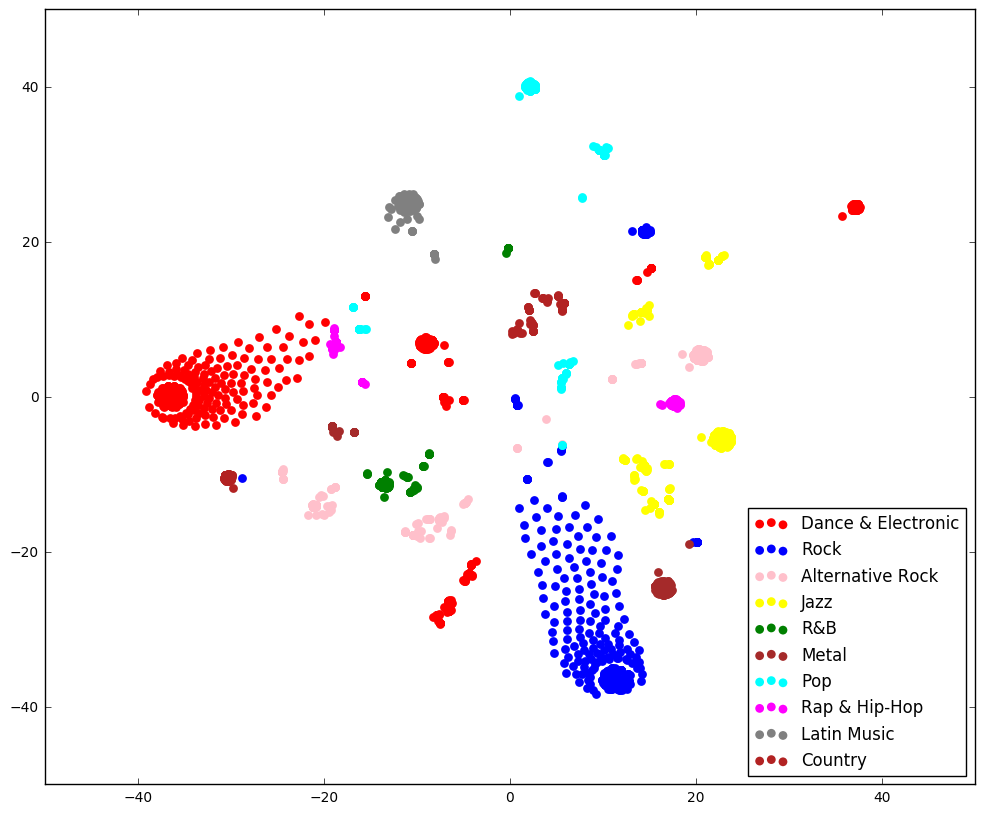
\includegraphics[width=0.9\columnwidth]{ch09_multi-class_pics/album_factors_train.png}}
\caption{t-SNE of album factors.}
\label{fig:tsne}
\end{figure}

The matrix of album genre annotations of the training and validation sets is factorized using the approach described in Section~\ref{sec:multi-class:factorization}, with a value of $d = 50$ dimensions.
From the set of album factors, those annotated with a single label from the top level of the taxonomy are plotted in Figure~\ref{fig:tsne} using t-SNE dimensionality reduction \citep{maaten2008visualizing}.
It can be seen how the different albums are properly clustered in the factor space according to their genre.


\subsection{Audio classification}\label{sec:multi-class:audioexp}

We explore three network design parameters: convolution filter size, number of filters per convolutional layer, and target layer. 
For the filter size we compare three approaches: square 3x3 filters as in \cite{Choi2016}, a filter of 4x96 that convolves only in time \citep{Oord2013}, and a musically motivated filter of 4x70, which is able to slightly convolve in the frequency domain \citep{pons2016experimenting}. 
To study the width of the convolutional layers we try with two different settings: \textsc{high} with 256, 512, 1024, and 1024 in each layer respectively, and \textsc{low} with 64, 128, 128, 64 filters. %We empirically set these two configurations. 
Max-pooling is applied after each convolutional layer.
Finally, we use the two different network targets defined in Section~\ref{sec:multi-class:multilabel}, \textsc{logistic} and \textsc{cosine}. %Moreover, we studied how the use of Dropout regularization \cite{} affect both target configurations.
We empirically observed that dropout regularization only helps in the \textsc{high} plus \textsc{cosine} configurations. Therefore we applied dropout with a factor of 0.5 to these configurations, and no dropout to the others. %The dataset is standarized with zero mean and unit variance.

Apart from these configurations, a baseline approach is added. This approach consists in a traditional audio-based approach for genre classification based on the audio descriptors present in the MSD \citep{Bertin-Mahieux2011}.
More specifically, for each song we aggregate four different statistics of the 12 timbre coefficient matrices: mean, max, variance, and $l2$-norm.
The obtained 48 dimensional feature vectors are fed into a feed forward network as the one described in Section~\ref{sec:multi-class:multimodal} with \textsc{logistic} output.
This approach is denoted as \textsc{timbre-mlp}.
%Second, we added a state-of-the-art multi-label genre classification approach based on the combination of convolutional and recurrent neural networks \cite{Keun2} whose source code is available\footnote{\url{https://github.com/keunwoochoi/music-auto_tagging-keras}}. We computed the mel-spectrograms with the provided code and trained the model using the exact same architecture, just changing the size of the output layer match the number of genre labels.

%Results of the different approaches are reported in Table~\ref{tbl:audio}. 

The results show that CNNs applied over audio spectrograms clearly outperform traditional approaches based on handcrafted features. 
We observe that the \textsc{timbre-mlp} approach achieves 0.792 of AUC, contrasting with the 0.888 from the best CNN approach.
We note that the \textsc{logistic} configuration obtains better results when using a lower number of filters per convolution (\textsc{low}). Configurations with fewer filters have less parameters to optimize, and their training processes are faster. 
On the other hand, in \textsc{cosine} configurations we observe that the use of a higher number of filters tends to achieve better performance. 
It seems that the fine-grained regression of the factors benefits from wider convolutions.
Moreover, we observe that 3x3 square filter settings have lower performance, need more time to train, and have a higher number of parameters to optimize.
By contrast, networks using time convolutions only (\textsc{4x96}) have a lower number of parameters, are faster to train, and achieve comparable performance. 
Furthermore, networks that slightly convolve across the frequency bins (\textsc{4x70}) achieve better results with only a slightly higher number of parameters and training time. 
Finally, we observe that the \textsc{cosine} regression approach achieves better AUC scores in most configurations, and also their results are more diverse in terms of aggregated diversity.

%As described in Section~\ref{}, album feature vectors are created by averaging the feature vectors of the different tracks of an album. In Table~\ref{} we evaluate this approach by comparing different strategies for feature aggregation. We compare these strategies in the \textsc{logistic/low-4x70} and \textsc{cosine/high-4x70} respectively. We observe in the results that the average outperform the maximum and the random selection of a track feature vector.

%(TODO: Tabla)

\subsection{Text classification}\label{sec:multi-class:textexp}

For text classification, we obtain two feature vectors as described in Section~\ref{sec:multi-class:text}: one built from the texts (\textsc{VSM}), and another built from the semantically enriched texts (\textsc{VSM+Sem}). 
Both feature vectors are trained in the multi-label genre classification task using the two output configurations \textsc{logistic} and \textsc{cosine}.

Results show that the semantic enrichment of texts clearly yields better results in terms of AUC and diversity.
Furthermore, we observe that the \textsc{cosine} configuration slightly outperforms \textsc{logistic} in terms of AUC, and greatly in terms of aggregated diversity. 
The text-based results are overall slightly superior than the audio-based ones. 

We also studied the information gain of words in the different genres. We observed that genre labels present inside the texts have high information gain values. It is also remarkable that \textit{band} is a very informative word for Rock, \textit{song} for Pop, and \textit{dope}, \textit{rhymes}, and \textit{beats} are discriminative features for Rap albums. Place names have also important weights, as \textit{Jamaica} for Reggae, \textit{Nashville} for Country, or \textit{Chicago} for Blues.%\footnote{The complete list of words is available on-line at https://www.upf.edu/en/web/mtg/mumu}.

%%%ADD TABLE and ref

\subsection{Image classification}\label{sec:multi-class:imageexp}


\begin{figure}
\centering
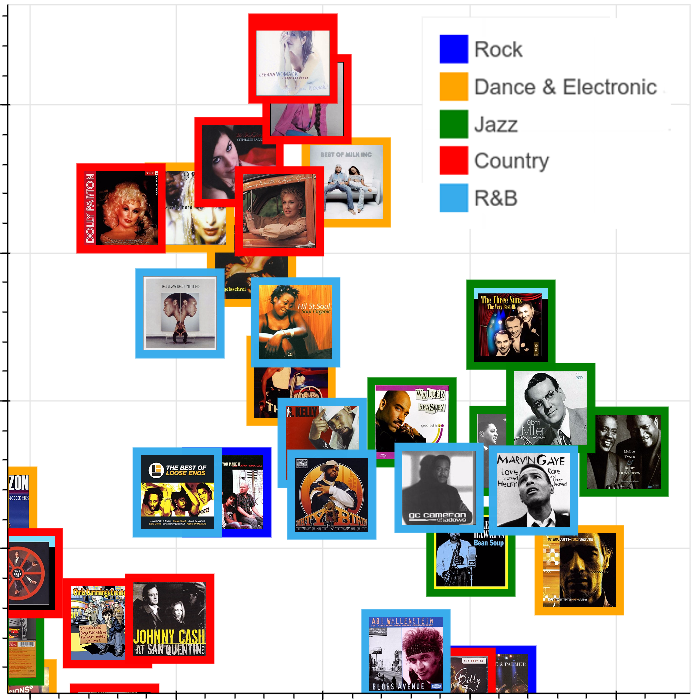
\includegraphics[height=8cm,keepaspectratio]{ch09_multi-class_pics/visual_zoom2.png} \\ 
\caption{Particular of the t-SNE of randomly selected image vectors from five of the most frequent genres.}
\label{fig:tsne_visual}
\end{figure}

%(TODO: We need better consistency: these parameters should go in the previous section, as with the ones of audio. Alternative, you can move those from section 5.1 to 6.1).
Results show that genre classification from images has lower performance in terms of AUC and aggregated diversity compared to the other modalities. Due to the use of an already pre-trained network with a logistic output (ImageNet \cite{ILSVRC15}) as initialization of the network, it is not straightforward to apply the \textsc{cosine} configuration. Therefore, we only report results for the \textsc{logistic} configuration.

In Figure~\ref{fig:tsne_visual} a set of cover images of five of the most frequent genres in the dataset is shown using t-SNE over the obtained image feature vectors. 
In the left top corner the ResNet recognizes women faces on the foreground, which seems to be common in Country albums (red).
%Also the R\&B genre appears to be generally well clustered, since black men that the network sucessfully recognizes tend to appear on the cover. 
The jazz albums (green) on the right are all clustered together probably thanks to the uniform type of clothing worn by the people of their covers. 
% In general, the visual content can give us relevant information about the singer, and this can be very informative. %(like for the African-American in R\&B, or also in Rap \& Hip Hop where the singer often wear a backwards hats).
Therefore, the visual style of the cover seems to be informative when recognizing the album genre.
For instance, many classical music albums include an instrument in the cover, and Dance \& Electronics covers are often abstract images with bright colors, rarely including human faces.

\subsection{Multimodal classification}\label{sec:multi-class:multiexp}

From the best performing approaches in terms of AUC of each modality (i.e., \textsc{Audio}/\textsc{cosine}/\textsc{high-4x70}, \textsc{Text}/\textsc{cosine}/\textsc{VSM+Sem} and \textsc{Image}/\textsc{logistic}/\textsc{ResNet}), an internal feature representation is obtained as described in Section~\ref{sec:multi-class:multimodal}. 
Then, these three feature vectors are aggregated in all possible combinations, and genre labels are predicted using the MLP network described in Section~\ref{sec:multi-class:multimodal}.
Both output configurations \textsc{logistic} and \textsc{cosine} are used in the learning phase, and dropout of 0.7 is applied in the \textsc{cosine} configuration.
%Although a feature vector can be extracted from a network trained with \textsc{cosine} configuration (e.g. \textsc{Audio} / \textsc{cosine} / \textsc{high-4x70}), when this vector is used in a multimodal approach, the multimodal network can be either trained with \textsc{logistic} or \textsc{cosine} configurations. The same happens with vectors trained with \textsc{logistic} loss.

Results suggest that the combination of modalities outperforms single modality approaches. 
As image features are learned using a \textsc{logistic} configuration, they seem to improve multimodal approaches with \textsc{logistic} configuration only. 
Multimodal approaches that include text features tend to achieve better results. %, even if the difference in performance between the different combinations is not pronounced.
Nevertheless, the best approaches are those that exploit the three modalities of \emph{MuMu}. \textsc{Cosine} approaches have similar AUC than \textsc{logistic} approaches but a much better aggregated diversity, thanks to the spatial properties of the factors space. 

%Album factors tend to be near their associated genre factors in the latent space, and similar genres are grouped together. Therefore, when an album factor is predicted by the network, the nearest genres in the space achieve the highest probability score. Although popular genre factors may have some hub properties in the latent space \cite{radovanovic2010hubs}, they can not be nearest neighbor of the majority of album factors. However, in the \textsc{logistic} configuration, it is easy for the network to prioritize one specific output that is very popular in the dataset (e.g. Pop or Rock), because this warranties a reduction of the crossentropy loss.

\section{Conclusions}\label{sec:multi-class:conclusions}

An approach for multi-label music genre classification using deep learning architectures has been proposed. 
The approach was applied to audio, text, and image data, and to the combination of learned data representations. 
For its assessment, \emph{MuMu}, a new multimodal music dataset with over 31k albums and 147k songs has been gathered. 
% This dataset encompasses multimodal information of about . Results show how the different modalities behave in the task. 
We showed how representation learning approaches for audio classification outperform traditional handcrafted feature based approaches.
Moreover, we compared the effect of different design parameters of CNNs in audio classification. 
Text-based approaches seem to outperform other modalities, and benefit from the semantic enrichment of texts via entity linking. %, helping reduce the gap between audio- and text-based approaches.
% However, compared with previous research in the field, the gap between audio and text-based approaches has been reduced. 
% This has been possible thanks to the introduction of deep learning approaches. 
While the image-based classification yielded the lowest performance, it helped to improve the results when combined with other modalities.
Multimodal approaches appear to outperform single modality approaches, and the aggregation of the three modalities achieved the best results.
Furthermore, the dimensionality reduction of target labels led to better results, not only in terms of accuracy, but also in terms of aggregated diversity.

The work in this chapter is an initial attempt to study the multi-label classification problem of music genres from different perspectives and using different data modalities. In addition, the release of the \emph{MuMu} dataset opens up a number of unexplored research possibilities. %In the near future we aim to modify the ResNet to be able to learn latent factors from images as we did in other modalities and apply the same multimodal approach to other MIR tasks.
\cleartorecto%!TEX root = ../thesis_a4.tex
\addtocontents{toc}{\protect\addvspace{2.25em plus 1pt}}
\bookmarksetup{startatroot}

\chapter{Summary and future perspectives}
\label{sec:conclusion}

\section{Introduction}

When the work for this thesis was initially developed, there was almost no published literature related with the extraction of high level semantic representations from music unstructured texts, although, in the context of MIR, a growing number of research works exploiting user generated texts (\cite{Celma2006,lamere2008social,Whitman2002,Knees2013}), and online knowledge repositories (\cite{sordo1788,Celma:ISWC06,dbrec1,Ostuni2013}) had been published. Initial attempts to apply knowledge extraction techniques to the music domain (\cite{Tata2010,Knees2011,Sordo2012}), showed the epistemic potential of text for music applications. In this thesis we have followed these ideas, deepening in the linguistic processing applied to extract the information, and proposing new approaches that exploit the extracted information in MIR tasks such as music recommendation and classification. In addition, we have combined extracted semantic information with content from other data modalities such as audio and images using deep neural networks. New data representations learned from the different data modalities and their combination have shown to outperform traditional hand-crafted audio features and single modality approaches.

We started this dissertation motivating and framing it with an introduction to knowledge extraction and representation learning in the context of MIR. In addition, we introduced the music recommendation and classification tasks (Chapter~\ref{sec:intro}). We continued by illustrating some background concepts related to Natural Language Processing and summarizing the existing literature on text-based, knowledge-based, and deep learning approaches in the context of MIR and Recommender Systems. Then, we described a framework for entity linking and the creation of a large corpus of annotated musical entities (Chapter~\ref{sec:linking}). We next proposed a method for extracting semantic relations between musical entities present in unstructured texts, and we evaluated the suitability of extracted knowledge to provide explanations for music recommendations (Chapter~\ref{sec:kb}). Two experiments on the applications of knowledge extraction for musicological studies were exposed next (Chapter~\ref{sec:musicology}). Then, we presented several knowledge-based approaches for artist similarity and music classification (Chapter\ref{sec:similarity}), and also for music recommendation (Chapter~\ref{sec:graph-rec}). Finally, we described a multimodal deep learning approach applied to cold-start music recommendations (Chapter~\ref{sec:cold-rec}), and to multi-label music genre classification (Chapter~\ref{sec:multi-class}).

In each chapter, we provided a summary of the conclusions and relevant results of the corresponding work. In what follows, we enumerate the main contribution of this thesis. Finally, we end this dissertation with a discussion about future research directions.

\section{Summary of contributions}
\label{sec:conclusion:summary}

In this thesis, we have focused on the problem of recommending and classifying musical items in large music collections applying two different approaches: (i) an approach based on the extraction of structured knowledge from unstructured texts and its further enrichment using semantic information coming from online knowledge repositories, (ii) an approach based on representation learning from multimodal data using deep learning architectures. We now present a summary of the main contributions of this thesis.

\subsection{Scientific Contributions}

\begin{enumerate}

\item 
A comprehensive review of current approaches in Natural Language Processing, Recommender Systems, and Music Information Retrieval, with a special focus on entity linking, knowledge base creation, relation extraction, artist similarity, music classification, and music recommendation (Chapter~\ref{sec:SOA}).

%\item 
%A system that integrates different entity linking tools, providing high confident entity disambiguations. The system is further leveraged for the creation of a novel benchmarking dataset of annotated musical entities, which are in turn linked to DBpedia and MusicBrainz. From this corpus, a gold standard dataset of manually annotated entities is also created.

\item 
An approach for the automatic creation of music knowledge bases from unstructured texts, which encodes semantic relations among musical entities, leveraging syntactic, and semantic information (Chapter~\ref{sec:kb}). % Our method relies on the syntactic structure of sentences and the use and adaptation of music-specific heuristics for both \textsc{EL} and \textsc{RE}. %In addition, we include modules for semantic clustering and pattern scoring, aimed at the efficient removal of noisy relations. 
The approach has the following advantages:

\begin{enumerate}
\item 
It is able to capture a highly precise and compact set of weighted triples thanks to a clustering method and a novel scoring metric. 
\item 
Given a proper text corpora, it is able to extract knowledge not present in other knowledge bases, both general and domain-specific. 
\item
The extracted knowledge base is suitable to provide explanations for music recommendations.
\end{enumerate}

\item 
An exploratory study on how knowledge extraction techniques may impact musicological studies (Chapter~\ref{sec:musicology}), which has produced the following outcomes:
\begin{enumerate}
\item 
An approach for the creation of culture-specific Music Knowledge Bases, which combines structured information coming from different data sources and information extracted from unstructured texts. 
\item
A methodology to build knowledge graphs from unstructured texts suitable for computing artist's relevance.
\item 
A method to extract and analyze the sentiment polarity expressed in music reviews, which is used to study the evolution of music genres and affective language.
%A diachronic study of the sentiment polarity expressed in album customer reviews, which suggests that non-music related circumstances may influence the way people speak about music, and demonstrate its usefulness to analyze the evolution of music genres.
\end{enumerate}

\item 
A methodology for the enrichment of unstructured text documents with information present in online knowledge repositories and their further exploitation in artist similarity and music classification tasks, outperforming traditional text-based approaches (Chapter~\ref{sec:similarity}).

\item
An extension of the previous contribution for the creation of knowledge graphs from tags and item's descriptions leveraging semantic information. These graphs are in turn exploited together with user's feedback information in a hybrid recommendation approach. An extensive evaluation shows improvements with respect to state-of-the-art collaborative filtering algorithms, in terms of prediction accuracy, novelty, and aggregated diversity (Chapter~\ref{sec:graph-rec}).%  and other content-based baselines from various points of view such as prediction accuracy and catalog coverage, promoting long tail recommendations.

\item 
An approach to provide recommendations of novel artists and songs, combining audio tracks, semantically enriched artist biographies, and user feedback information using deep neural networks (Chapter~\ref{sec:cold-rec}). The proposed approach benefits from the late fusion of feature embeddings learned separately. %Following this approach, a recommender system is able to include songs of novel artists in its recommendations with higher accuracy 

%Results suggest that both splitting the recommendation problem between feature levels, and the late fusion of feature embeddings improve the accuracy of the recommendations, and outperforms end-to-end multimodal approaches where the different modalities are learned simultaneously.
%Moreover, deep learning architectures have demonstrated their capacity to improve upon other learning models under the music recommendation framework. 
%Results have shown that our multimodal approach achieves better results than pure text or audio approaches. 

\item 
A methodology for the simultaneous classification of multiple genre labels from audio, text, semantic information, images, and their combination using deep learning architectures. In the described approach, classification accuracy and aggregated diversity are improved by applying dimensionality reduction of target labels through matrix factorization techniques (Chapter~\ref{sec:multi-class}). %Additionally, a large multimodal dataset used for evaluation is released.

\end{enumerate}

\subsection{Contributions to Creating Datasets}

Adequate datasets to evaluate our approaches were not always available, so we have dedicated an important effort in gathering and curating new datasets. We describe below the specific contributions. 

\begin{enumerate}

\item 
Novel dataset of \~13k documents and almost 150k annotated musical entities, which are in turn linked to DBpedia and MusicBrainz. From this corpus, a gold standard dataset of 200 documents with manually annotated entities is also created (Section~\ref{sec:linking:lastfm}).

\item
Large dataset of about 64k albums with customer reviews, track acoustic features, metadata, and single-label genre annotations (Sections ~\ref{sec:musicology:mard} and \ref{sec:similarity:mard}).

\item
Two datasets of 188 and 2,336 artist biographies respectively, together with artist similarity ground truth data (Section ~\ref{sec:similarity:experimentalsetup}).

\item
Two datasets of tags and text descriptions about musical items, together with user feedback information on those items. A dataset of sounds with \~21k items and 20k users, and a dataset of songs with \~8.5k items and \~5k users (Section ~\ref{sec:graph-rec:datasets}).

\item
Dataset of \~24k artist biographies linked to the artists present in the Million Song Dataset (Section ~\ref{sec:cold-rec:dataset}).

\item
Large dataset of about \~31k albums, with \~450k customer reviews, \~147k audio tracks, cover artworks, and multi-label genre annotations (Section ~\ref{sec:multi-class:mumu}).

\end{enumerate}

\subsection{Contributions to Creating Music Knowledge Bases}

\begin{enumerate}
\item
A Music Knowledge Base of popular music extracted from a corpus of \~32k documents with stories about songs (Section~\ref{sec:kb:exp:learnedkbs}).

\item
A Music Knowledge Base of flamenco music, created by combining data from 7 different data sources, and enriched with information extracted from \~1k artist biographies (Section~\ref{sec:musicology:flabase}).

\end{enumerate}

\subsection{Software Contributions}

\begin{enumerate}
\item
A system that integrates different entity linking tools, providing high confident entity disambiguations.

\item
A system to perform and evaluate deep learning experiments on classification and recommendation from different data modalities and their combination. %, and to obtain feature vectors from intermediate layers after training. 

\end{enumerate}

\subsection{Publications}
\label{sec:conclusion:publications}

The research carried out in this dissertation has been published in several peer reviewed journals and top international conferences. Parts of the research presented in Chapter~\ref{sec:linking} has been published in a conference paper \cite{Oramas2016}. The work described in Chapter~\ref{sec:kb} has been published in a conference and a journal paper \cite{Oramas2015,Oramas2016a}. The work described in this chapter is a joint effort by the author of this dissertation, and Luis Espinosa-Anke, both researchers in the Department of Information and Comunication Technologies of the Universitat Pompeu Fabra, Barcelona, framed within the Maria de Maetzu strategic excellence program. The parts of the research presented in Chapter~\ref{sec:musicology} related with the creation of domain-specific knowledge bases have been published in a conference and a journal paper \cite{Oramas2015b,}, and those related with the diachronic study of music reviews were published in another conference paper \cite{oramas2016exploring}. Similarly, the parts of the research presented in Chapter~\ref{sec:similarity} related with artist similarity have been published in a conference paper \cite{Oramas2015a}, and those related with music genre classification have been published in \cite{oramas2016exploring}. Furthermore, the outcomes of Chapter~\ref{sec:graph-rec} have been published in a conference and a journal paper \cite{Ostuni2015,oramas2016sound}. Finally, the work described in Chapter~\ref{sec:cold-rec} have been published in a conference paper \cite{}, and the outcomes of the research carried out in Chapter~\ref{sec:multi-class} have been published in a conference paper \cite{}. The full list of author's publications related to the work presented in this thesis is available in Appendix A, and the full list of released datasets and software is available in Appendix B.


\section{Directions for future research}
\label{sec:conclusion:future}

In the present thesis we have tried to help machines to better understand what people have to say about music, and we have shown how to combine semantic knowledge, texts, user feedback, audio, and images in the context of MIR and computational musicology. This is an exploratory work that opens up a number of research possibilities for text-based and multimodal approaches in the music domain. In what follows, we enumerate a series of ideas for future work related with the different task addressed in this dissertation.

\paragraph{Entity Linking} As observed in Chapters~\ref{sec:linking} and \ref{sec:kb}, identification and classification of music entities in text is a problem far from being solved. Current systems make an important number of mistakes and do not operate on music specific knowledge bases, but on general purpose ones such as DBpedia or BabelNet. As availability of music entities in these knowledge bases is scarce, there is a need for an entity linking system able to recognize and disambiguate musical entities to a music knowledge base (e.g., MusicBrainz). We envision that splitting the problem into recognition and disambiguation may improve the precision. An entity recognizer trained with music specific corpora would benefit from the textual context of the entities to properly classify them. Then, categories identified by the recognizer would be used in the disambiguation step to improve the precision of linking. To this end, the creation of large datasets of annotated musical entities is a necessary step. %, that may be of interest of NLP researchers.

\paragraph{Construction of Knowledge Bases} In Chapter~\ref{sec:kb} we have explored the automatic creation of music knowledge bases using an approach based on the combination of open information extraction and entity linking. However, other approaches may be used, such as distant supervision. In the MusicBrainz database,  a large number of relations between entities are encoded together with information about the lexicalization of these relations. This is a highly valuable resource that can be exploited, for instance, in distant supervision approaches. Additionally, the creation of an open music knowledge base that constantly reads from the web, like the Never-Ending Language Learning system (NELL) (\cite{Carlson2010a}), would create a highly valuable resource, not only for research, but also for commercial applications.

\paragraph{Other NLP Techniques} In this work we have explored the application of several NLP techniques and tasks to the music domain. Among the tasks not explored in this thesis, we may highlight \textit{Question \& Answering}, which is a challenging problem that also deals with semantic representations of text. \textit{Question \& Answering} systems or chat bots may have several applications to the music domain, such as knowledge dissemination, promotion of artists, or music recommendation. Big companies are currently working on their own conversational systems. Knowledge bases have been traditionally exploited by these systems, and more recently, deep learning approaches using RNNs and memory networks have shown promising results learning directly from conversations. Moreover, other deep learning techniques such as reinforcement learning, have shown the potential of combining knowledge bases and deep learning in conversational systems (\cite{andreas2016learning}).

\paragraph{Musicology}
In Chapter~\ref{sec:musicology} we left some hypothesis open about the evolution of the language used in music reviews. To demonstrate any of these hypothesis is a challenging problem. In addition, a more thorough study on the evolution of music genres could be done thanks to the compiled dataset. We have shown how knowledge extraction techniques may facilitate musicologists work. Therefore, the creation of specific tools to process large amounts of musicological documents, either in music digital libraries or private collections, is an open research path.

\paragraph{Deep Learning for Text} Word vector embeddings have revealed very useful in most NLP tasks (\cite{Collobert2011}), and they have been widely exploited within deep learning approaches. Hence, further exploration on architectures that exploit the potential of these word representations in MIR tasks is a clear research direction. Additionally, combining lexical semantics encoded in word vectors and explicit semantics encoded in knowledge bases is another open research path. Novel techniques, such as retrofitting (\cite{faruqui2014retrofitting}), work in this direction. In addition, recent developments, such as LSTM networks with attention, could be also applied in the context of our research.

\paragraph{Music Classification} In Chapter~\ref{sec:multi-class} we have shown how new feature representations can be learned in a multi-label genre classification task. Given the high granularity of the genre annotations, learned features encode fine-grained properties of the data. Therefore, they might be exploited in other applications via transfer learning, such as music similarity or music recommendation. 

\paragraph{Music Recommendation} Common multimodal spaces can be learned from the feature vectors of different modalities. Mapping feature vectors in a common space may be useful to pass from one modality to another. One application of this may be, for instance, going from text to a set of audio tracks, giving rise to a new method for playlist generation.

\paragraph{Multimodal Deep Learning}
The multimodal deep learning approach presented in this thesis, is based on the late fusion of learned data representations. We have shown how this approach outperforms simultaneous learning from text and audio. However, an intermediate way would be to learn feature vectors separately, but then try to fine-tune the whole multimodal network in the final task, becoming a fully end-to-end learning approach.

\paragraph{Generative Models} Another intersting line of research we envision are generative models based on multimodal data. Generation of audio from text descriptions, text descriptions from audio, or album cover artwork from album tracks are some of the possible application. Similar approaches have already been developed for texts and images. However, the generation of/from audio has received lesser attention.

The writing of this thesis has been an exciting path through different ways of incorporating further human knowledge about music into computational systems.


\backmatter
\cleartorecto\cleartorecto
\pagestyle{empty}
\vspace*{\fill}
\cleanlookdateon
\begin{flushright}
Sergio Oramas Martín, Barcelona,  21 September 2017. %\today.
\end{flushright}

%\bibliographystyle{plainnat}
%\bibliographystyle{apa}
%\bibliographystyle{apa_jserra}
\bibliographystyle{apa_jserra2}
\cleartorecto\bibliography{biblio_final}
%\cleartorecto\small\bibliography{ch99/jserra}\normalsize
%\cleartorecto\footnotesize\bibliography{ch99/jserra}\normalsize


\let\svaddcontentsline\addcontentsline
\renewcommand\addcontentsline[3]{%
  \ifthenelse{\equal{#1}{lof}}{}%
  {\ifthenelse{\equal{#1}{lot}}{}{\svaddcontentsline{#1}{#2}{#3}}}}

\appendix
\cleartorecto%!TEX root = ../thesis_a4.tex

\chapter{Appendix B: publications by the author}
\label{sec:Pubs}


\section*{In press}


\section*{Journal papers}


Oramas S., Espinosa-Anke L., Sordo M., Saggion H. \& Serra X. (2016). Information Extraction for Knowledge Base Construction in the Music Domain. \emph{Data \& Knowledge Engineering, Volume 106}, Pages 70-83.

\vspace{0.2cm}

Oramas S., Ostuni V. C., Di Noia T., Serra, X., \& Di Sciascio E. (2016). Music and Sound Recommendation with Knowledge Graphs. \emph{ACM Transactions on Intelligent Systems and Technology, Volume 8}, Issue 2, Article 21.

\vspace{0.2cm}

Oramas S., Sordo M. (2016). Knowledge is Out There: A New Step in the Evolution of Music Digital Libraries. \emph{Fontes Artis Musicae, Vol 63, no. 4}.


\section*{Conference papers}

Oramas S., Espinosa-Anke L., Lawlor A., Serra X., \& Saggion H. (2016). Exploring Music Reviews for Music Genre Classification and Evolutionary Studies. \emph{In Proceedings of the 17th International Society for Music Information Retrieval Conference (ISMIR 2016)}.

\vspace{0.2cm}

Oramas S., Espinosa-Anke L., Sordo M., Saggion H., \& Serra X. (2016). ELMD: An Automatically Generated Entity Linking Gold Standard in the Music Domain. \emph{In Proceedings of the 10th Conference on Language Resources and Evaluation (LREC 2016)}.

\vspace{0.2cm}

Espinosa-Anke, L., Oramas S., Camacho-Collados J., \& Saggion H. (2016). Finding and Expanding Hypernymic Relations in the Music Domain. \emph{In Proceedings of the 19th International Conference of the Catalan Association for Artificial Intelligence (CCIA 2016)}.

\vspace{0.2cm}

Oramas S., Sordo M., Espinosa-Anke L., \& Serra X. (2015). A Semantic-based approach for Artist Similarity. \emph{In Proceedings of the 16th International Society for Music Information Retrieval Conference (ISMIR 2015)}.

\vspace{0.2cm}

Oramas S., Gómez F., Gómez E., \& Mora J. (2015). FlaBase: Towards the creation of a Flamenco Music Knowledge Base. \emph{In Proceedings of the 16th International Society for Music Information Retrieval Conference (ISMIR 2015)}.

\vspace{0.2cm}

Ostuni V. C., Oramas S., Di Noia T., Serra, X., \& Di Sciascio E. (2015). A Semantic Hybrid Approach for Sound Recommendation. \emph{In Proceedings of the 24th International World Wide Web Conference (WWW 2015, Poster track)}.

\vspace{0.2cm}

Oramas S., Sordo M., \& Espinosa-Anke L. (2015). A Rule-based Approach to Extracting Relations from Music Tidbits. \emph{In Proceedings of the 2nd Workshop on Knowledge Extraction from Text (KET 2015)}.

\vspace{0.2cm}

Sordo, M., Oramas S., \& Espinosa-Anke L. (2015). Extracting Relations from Unstructured Text Sources for Music Recommendation. \emph{In Proceedings of the 20th International Conference on Applications of Natural Language to Information Systems (NLDB 2015)}.

\vspace{0.2cm}

Oramas S., Sordo M., \& Serra X. (2014). Automatic Creation of Knowledge Graphs from Digital Musical Document Libraries. \emph{In Proceedings of the 9th Conference on Interdisciplinary Musicology (CIM 2014)}.

\vspace{0.2cm}

Oramas S. (2014). Harvesting and Structuring Social Data in Music Information Retrieval. \emph{In Proceedings of the Extended Semantic Web Conference (ESWC 2014, PhD Symposium)}.

\vspace{0.2cm}

Font, F., Oramas, S., Fazekas, G., \& Serra, X. (2014). Extending Tagging Ontologies with Domain Specific Knowledge. In \emph{Proceedings of the International Semantic Web Conference (ISWC 2014, Poster track)}.


\section*{Tutorials and Challenges}

Oramas S., Espinosa-Anke L., Zhang S., Saggion H., \& Serra X. (2016). Natural Language Processing for Music Information Retrieval. \emph{17th International Society for Music Information Retrieval Conference (ISMIR 2016)}.


\section*{Conference presentations}

Oramas, S. (2017). Discovering Similarities and Relevance Ranking of Renaissance Composers. \emph{The 63rd Annual Meeting of the Renaissance Society of America (RSA)}, Chicago.

\vspace{0.2cm}

Oramas S. (2015). Information Extraction for the Music Domain. \emph{The 2nd International Workshop on Human History Project: Natural Language Processing and Big Data}, CIRMMT, Montreal.

\vspace{0.2cm}

Oramas, S., \& Sordo M. (2015). Knowledge Acquisition from Music Digital Libraries. \emph{The International Association of Music Libraries and International Musicological Society Conference (IAML/IMS 2015)}, New York.


\cleartorecto%!TEX root = ../thesis_a4.tex

\chapter{Appendix B: Datasets and Knowledge Bases}
\label{appendix:datasets}

\section{Datasets}
\label{appendix:datasets:datasets}

\noindent \textbf{ELMD} Dataset of $\sim$13k documents and almost 150k annotated musical entities, which are linked to DBpedia and MusicBrainz. From this corpus, a gold standard dataset of 200 documents with manually annotated entities is also created (Section~\ref{sec:linking:lastfm}). \url{http://mtg.upf.edu/download/datasets/elmd}

\vspace{0.2cm}

\noindent \textbf{MARD} Large dataset of about 64k albums with customer reviews, acoustic features per track, metadata, and single-label genre annotations (Sections ~\ref{sec:musicology:mard} and \ref{sec:similarity:mard}). \url{http://mtg.upf.edu/download/datasets/mard}

\vspace{0.2cm}

\noindent \textbf{SAS} Two datasets of 188 and 2,336 artist biographies respectively, together with artist similarity ground truth data (Section ~\ref{sec:similarity:experimentalsetup}). \url{http://mtg.upf.edu/download/datasets/semantic-similarity}

\vspace{0.2cm}

\noindent \textbf{KG-Rec} Two datasets of tags and text descriptions about musical items, together with user feedback information on those items. A dataset of sounds with $\sim$21k items and 20k users, and a dataset of songs with $\sim$8.5k items and $\sim$5k users (Section ~\ref{sec:graph-rec:datasets}). \url{http://mtg.upf.edu/download/datasets/knowledge-graph-rec}

\vspace{0.2cm}

\noindent \textbf{MSD-A} Dataset of $\sim$24k artist biographies linked to the artists present in the Million Song Dataset (Section ~\ref{sec:cold-rec:dataset}). \url{http://mtg.upf.edu/download/datasets/msd-a}

\vspace{0.2cm}

\noindent \textbf{MuMu} Large dataset of about $\sim$31k albums, with $\sim$450k customer reviews, $\sim$147k audio tracks, cover artworks, and multi-label genre annotations (Section ~\ref{sec:multi-class:mumu}). \url{https://www.upf.edu/web/mtg/mumu}

\section{Knowledge Bases}

\noindent \textbf{KBSF} Music Knowledge Base of popular music extracted from a corpus of $\sim$32k documents with stories about songs (Section~\ref{sec:kb:exp:learnedkbs}). \url{http://mtg.upf.edu/download/datasets/kbsf}

\vspace{0.2cm}

\noindent \textbf{FlaBase} Music Knowledge Base of flamenco music, created by combining data from 7 different data sources, and enriched with information extracted from $\sim$1k artist biographies (Section~\ref{sec:musicology:flabase}). \url{http://mtg.upf.edu/download/datasets/flabase}


\section{Software}

\noindent \textbf{ELVIS} System that integrates different entity linking tools, providing high confident entity disambiguations. \url{https://github.com/sergiooramas/elvis}

\vspace{0.2cm}

\noindent \textbf{Tartarus} System to perform and evaluate deep learning experiments on classification and recommendation from different data modalities and their combination. \url{https://github.com/sergiooramas/tartarus}
 
%\cleartorecto\include{ch99/quotation}
\cleartorecto\newpage\thispagestyle{empty}\mbox{}
%\cleartorecto\newpage\thispagestyle{empty}\mbox{}

\end{document}

%------------------------------------------------------------------------------------------------
% -----------------------------------------------------------------------------------------------
%------------------------------------------------------------------------------------------------
%------------------------------------------------------------------------------------------------
